% Generated by Sphinx.
\def\sphinxdocclass{report}
\documentclass[A4paperpaper,11pt,english]{sphinxmanual}
\usepackage[utf8]{inputenc}
\DeclareUnicodeCharacter{00A0}{\nobreakspace}
\usepackage{cmap}
\usepackage[T1]{fontenc}
\usepackage{babel}
\usepackage{times}
\usepackage[Bjarne]{fncychap}
\usepackage{longtable}
\usepackage{sphinx}
\usepackage{multirow}

\usepackage{pdfpages}
\setcounter{tocdepth}{2}
% \makeatletter
% \def\cleardoublepage{
% \clearpage\if@twoside \ifodd\c@page\else
% \hbox{}
% \vspace*{\fill}
% \vspace{\fill}
% \thispagestyle{empty}
% \newpage
% \if@twocolumn\hbox{}\newpage\fi\fi\fi
% }
% \makeatother

\renewcommand{\maketitle}{}


\title{Actin Gels dynamics}
\date{May 17, 2015 at 09:11:12 PDT}
\release{}
\author{Matthias Bussonnier}
\newcommand{\sphinxlogo}{}
\renewcommand{\releasename}{}
\makeindex

\makeatletter
\def\PYG@reset{\let\PYG@it=\relax \let\PYG@bf=\relax%
    \let\PYG@ul=\relax \let\PYG@tc=\relax%
    \let\PYG@bc=\relax \let\PYG@ff=\relax}
\def\PYG@tok#1{\csname PYG@tok@#1\endcsname}
\def\PYG@toks#1+{\ifx\relax#1\empty\else%
    \PYG@tok{#1}\expandafter\PYG@toks\fi}
\def\PYG@do#1{\PYG@bc{\PYG@tc{\PYG@ul{%
    \PYG@it{\PYG@bf{\PYG@ff{#1}}}}}}}
\def\PYG#1#2{\PYG@reset\PYG@toks#1+\relax+\PYG@do{#2}}

\expandafter\def\csname PYG@tok@gi\endcsname{\def\PYG@tc##1{\textcolor[rgb]{0.00,0.63,0.00}{##1}}}
\expandafter\def\csname PYG@tok@mh\endcsname{\def\PYG@tc##1{\textcolor[rgb]{0.13,0.50,0.31}{##1}}}
\expandafter\def\csname PYG@tok@no\endcsname{\def\PYG@tc##1{\textcolor[rgb]{0.38,0.68,0.84}{##1}}}
\expandafter\def\csname PYG@tok@mb\endcsname{\def\PYG@tc##1{\textcolor[rgb]{0.13,0.50,0.31}{##1}}}
\expandafter\def\csname PYG@tok@si\endcsname{\let\PYG@it=\textit\def\PYG@tc##1{\textcolor[rgb]{0.44,0.63,0.82}{##1}}}
\expandafter\def\csname PYG@tok@gu\endcsname{\let\PYG@bf=\textbf\def\PYG@tc##1{\textcolor[rgb]{0.50,0.00,0.50}{##1}}}
\expandafter\def\csname PYG@tok@s2\endcsname{\def\PYG@tc##1{\textcolor[rgb]{0.25,0.44,0.63}{##1}}}
\expandafter\def\csname PYG@tok@nn\endcsname{\let\PYG@bf=\textbf\def\PYG@tc##1{\textcolor[rgb]{0.05,0.52,0.71}{##1}}}
\expandafter\def\csname PYG@tok@vc\endcsname{\def\PYG@tc##1{\textcolor[rgb]{0.73,0.38,0.84}{##1}}}
\expandafter\def\csname PYG@tok@sx\endcsname{\def\PYG@tc##1{\textcolor[rgb]{0.78,0.36,0.04}{##1}}}
\expandafter\def\csname PYG@tok@kc\endcsname{\let\PYG@bf=\textbf\def\PYG@tc##1{\textcolor[rgb]{0.00,0.44,0.13}{##1}}}
\expandafter\def\csname PYG@tok@kn\endcsname{\let\PYG@bf=\textbf\def\PYG@tc##1{\textcolor[rgb]{0.00,0.44,0.13}{##1}}}
\expandafter\def\csname PYG@tok@c1\endcsname{\let\PYG@it=\textit\def\PYG@tc##1{\textcolor[rgb]{0.25,0.50,0.56}{##1}}}
\expandafter\def\csname PYG@tok@na\endcsname{\def\PYG@tc##1{\textcolor[rgb]{0.25,0.44,0.63}{##1}}}
\expandafter\def\csname PYG@tok@nt\endcsname{\let\PYG@bf=\textbf\def\PYG@tc##1{\textcolor[rgb]{0.02,0.16,0.45}{##1}}}
\expandafter\def\csname PYG@tok@cm\endcsname{\let\PYG@it=\textit\def\PYG@tc##1{\textcolor[rgb]{0.25,0.50,0.56}{##1}}}
\expandafter\def\csname PYG@tok@ow\endcsname{\let\PYG@bf=\textbf\def\PYG@tc##1{\textcolor[rgb]{0.00,0.44,0.13}{##1}}}
\expandafter\def\csname PYG@tok@nl\endcsname{\let\PYG@bf=\textbf\def\PYG@tc##1{\textcolor[rgb]{0.00,0.13,0.44}{##1}}}
\expandafter\def\csname PYG@tok@il\endcsname{\def\PYG@tc##1{\textcolor[rgb]{0.13,0.50,0.31}{##1}}}
\expandafter\def\csname PYG@tok@ni\endcsname{\let\PYG@bf=\textbf\def\PYG@tc##1{\textcolor[rgb]{0.84,0.33,0.22}{##1}}}
\expandafter\def\csname PYG@tok@kp\endcsname{\def\PYG@tc##1{\textcolor[rgb]{0.00,0.44,0.13}{##1}}}
\expandafter\def\csname PYG@tok@s1\endcsname{\def\PYG@tc##1{\textcolor[rgb]{0.25,0.44,0.63}{##1}}}
\expandafter\def\csname PYG@tok@mf\endcsname{\def\PYG@tc##1{\textcolor[rgb]{0.13,0.50,0.31}{##1}}}
\expandafter\def\csname PYG@tok@sd\endcsname{\let\PYG@it=\textit\def\PYG@tc##1{\textcolor[rgb]{0.25,0.44,0.63}{##1}}}
\expandafter\def\csname PYG@tok@bp\endcsname{\def\PYG@tc##1{\textcolor[rgb]{0.00,0.44,0.13}{##1}}}
\expandafter\def\csname PYG@tok@nc\endcsname{\let\PYG@bf=\textbf\def\PYG@tc##1{\textcolor[rgb]{0.05,0.52,0.71}{##1}}}
\expandafter\def\csname PYG@tok@kd\endcsname{\let\PYG@bf=\textbf\def\PYG@tc##1{\textcolor[rgb]{0.00,0.44,0.13}{##1}}}
\expandafter\def\csname PYG@tok@cp\endcsname{\def\PYG@tc##1{\textcolor[rgb]{0.00,0.44,0.13}{##1}}}
\expandafter\def\csname PYG@tok@m\endcsname{\def\PYG@tc##1{\textcolor[rgb]{0.13,0.50,0.31}{##1}}}
\expandafter\def\csname PYG@tok@sc\endcsname{\def\PYG@tc##1{\textcolor[rgb]{0.25,0.44,0.63}{##1}}}
\expandafter\def\csname PYG@tok@kt\endcsname{\def\PYG@tc##1{\textcolor[rgb]{0.56,0.13,0.00}{##1}}}
\expandafter\def\csname PYG@tok@nv\endcsname{\def\PYG@tc##1{\textcolor[rgb]{0.73,0.38,0.84}{##1}}}
\expandafter\def\csname PYG@tok@nd\endcsname{\let\PYG@bf=\textbf\def\PYG@tc##1{\textcolor[rgb]{0.33,0.33,0.33}{##1}}}
\expandafter\def\csname PYG@tok@sh\endcsname{\def\PYG@tc##1{\textcolor[rgb]{0.25,0.44,0.63}{##1}}}
\expandafter\def\csname PYG@tok@go\endcsname{\def\PYG@tc##1{\textcolor[rgb]{0.20,0.20,0.20}{##1}}}
\expandafter\def\csname PYG@tok@vg\endcsname{\def\PYG@tc##1{\textcolor[rgb]{0.73,0.38,0.84}{##1}}}
\expandafter\def\csname PYG@tok@mo\endcsname{\def\PYG@tc##1{\textcolor[rgb]{0.13,0.50,0.31}{##1}}}
\expandafter\def\csname PYG@tok@gs\endcsname{\let\PYG@bf=\textbf}
\expandafter\def\csname PYG@tok@gp\endcsname{\let\PYG@bf=\textbf\def\PYG@tc##1{\textcolor[rgb]{0.78,0.36,0.04}{##1}}}
\expandafter\def\csname PYG@tok@nb\endcsname{\def\PYG@tc##1{\textcolor[rgb]{0.00,0.44,0.13}{##1}}}
\expandafter\def\csname PYG@tok@se\endcsname{\let\PYG@bf=\textbf\def\PYG@tc##1{\textcolor[rgb]{0.25,0.44,0.63}{##1}}}
\expandafter\def\csname PYG@tok@w\endcsname{\def\PYG@tc##1{\textcolor[rgb]{0.73,0.73,0.73}{##1}}}
\expandafter\def\csname PYG@tok@ss\endcsname{\def\PYG@tc##1{\textcolor[rgb]{0.32,0.47,0.09}{##1}}}
\expandafter\def\csname PYG@tok@err\endcsname{\def\PYG@bc##1{\setlength{\fboxsep}{0pt}\fcolorbox[rgb]{1.00,0.00,0.00}{1,1,1}{\strut ##1}}}
\expandafter\def\csname PYG@tok@gh\endcsname{\let\PYG@bf=\textbf\def\PYG@tc##1{\textcolor[rgb]{0.00,0.00,0.50}{##1}}}
\expandafter\def\csname PYG@tok@nf\endcsname{\def\PYG@tc##1{\textcolor[rgb]{0.02,0.16,0.49}{##1}}}
\expandafter\def\csname PYG@tok@s\endcsname{\def\PYG@tc##1{\textcolor[rgb]{0.25,0.44,0.63}{##1}}}
\expandafter\def\csname PYG@tok@mi\endcsname{\def\PYG@tc##1{\textcolor[rgb]{0.13,0.50,0.31}{##1}}}
\expandafter\def\csname PYG@tok@ne\endcsname{\def\PYG@tc##1{\textcolor[rgb]{0.00,0.44,0.13}{##1}}}
\expandafter\def\csname PYG@tok@o\endcsname{\def\PYG@tc##1{\textcolor[rgb]{0.40,0.40,0.40}{##1}}}
\expandafter\def\csname PYG@tok@cs\endcsname{\def\PYG@tc##1{\textcolor[rgb]{0.25,0.50,0.56}{##1}}\def\PYG@bc##1{\setlength{\fboxsep}{0pt}\colorbox[rgb]{1.00,0.94,0.94}{\strut ##1}}}
\expandafter\def\csname PYG@tok@gr\endcsname{\def\PYG@tc##1{\textcolor[rgb]{1.00,0.00,0.00}{##1}}}
\expandafter\def\csname PYG@tok@gd\endcsname{\def\PYG@tc##1{\textcolor[rgb]{0.63,0.00,0.00}{##1}}}
\expandafter\def\csname PYG@tok@ge\endcsname{\let\PYG@it=\textit}
\expandafter\def\csname PYG@tok@vi\endcsname{\def\PYG@tc##1{\textcolor[rgb]{0.73,0.38,0.84}{##1}}}
\expandafter\def\csname PYG@tok@sb\endcsname{\def\PYG@tc##1{\textcolor[rgb]{0.25,0.44,0.63}{##1}}}
\expandafter\def\csname PYG@tok@sr\endcsname{\def\PYG@tc##1{\textcolor[rgb]{0.14,0.33,0.53}{##1}}}
\expandafter\def\csname PYG@tok@c\endcsname{\let\PYG@it=\textit\def\PYG@tc##1{\textcolor[rgb]{0.25,0.50,0.56}{##1}}}
\expandafter\def\csname PYG@tok@k\endcsname{\let\PYG@bf=\textbf\def\PYG@tc##1{\textcolor[rgb]{0.00,0.44,0.13}{##1}}}
\expandafter\def\csname PYG@tok@gt\endcsname{\def\PYG@tc##1{\textcolor[rgb]{0.00,0.27,0.87}{##1}}}
\expandafter\def\csname PYG@tok@kr\endcsname{\let\PYG@bf=\textbf\def\PYG@tc##1{\textcolor[rgb]{0.00,0.44,0.13}{##1}}}

\def\PYGZbs{\char`\\}
\def\PYGZus{\char`\_}
\def\PYGZob{\char`\{}
\def\PYGZcb{\char`\}}
\def\PYGZca{\char`\^}
\def\PYGZam{\char`\&}
\def\PYGZlt{\char`\<}
\def\PYGZgt{\char`\>}
\def\PYGZsh{\char`\#}
\def\PYGZpc{\char`\%}
\def\PYGZdl{\char`\$}
\def\PYGZhy{\char`\-}
\def\PYGZsq{\char`\'}
\def\PYGZdq{\char`\"}
\def\PYGZti{\char`\~}
% for compatibility with earlier versions
\def\PYGZat{@}
\def\PYGZlb{[}
\def\PYGZrb{]}
\makeatother

\renewcommand\PYGZsq{\textquotesingle}

\begin{document}

\maketitle
%%       \begin{center}
%%        \begin{minipage}{0.75\linewidth}
%%            \centering
%%            % \rule{0.4\linewidth}{0.15\linewidth}\par
%%            {\uppercase{\large \'Ecole Doctorale Mati\`ere Condend\'ee et interface \par}}
%%            {\uppercase{\large Laboratoire Physique Chimie du Vivant, Institut Curie, Umr 168 \par}}
%%            \vspace{2cm}
%%            {\uppercase{\Large  Doctorat \par}}
%%            {\uppercase{\Large  Physique \par}}
%%            \vspace{2cm}
%%           {\Large Bussonnier Matthias\par}
%%            \vspace{2cm}
%%            {\Large Actin Gel mechanics\par}
%%            {\Large Mechanique des gels d'actine\par}
%%            \vspace{2cm}
%%            \Large
%%            Th\`ese diri\'ee par Timo Betz et C\'ecile Sykes,\\
%%            Soutenue le 16 Septembre 2014\\
%%            \vspace{2cm}
%%                {\Large Jury}
%%            \vspace{1cm}
%%                \large
%%                \begin{flushleft}
%%                Prof. Atef Anacios , Pr\'esident\\
%%                Dr. Laurent Blanchoin\\
%%                Dr. Guillaume Rommet-Lemonne, Rapporteur\\
%%                Prof. Dr. Dr. Karsten Kruse, Rapporteur\\
%%                \end{flushleft}
%%
%%            \vspace{2cm}
%%        \end{minipage}
%%    \end{center}
%%    \newpage

    \begin{center}
        \begin{minipage}{0.75\linewidth}
    \begin{center}
            \noindent {\large \textbf{UNIVERSITÉ PARIS DIDEROT - SORBONNE PARIS CITÉ}} \\ 
            \vspace*{0.3cm}
            \noindent {\large \textbf{ÉCOLE DOCTORALE 518}} \\
            \noindent \textbf{CONDENSED MATTER \\ AND INTERFACES} \\
            \vspace*{0.5cm}
            \noindent \Huge \textbf{T H È S E} \\
            \vspace*{0.3cm}
            \noindent \large {pour obtenir le grade de} \\
            \vspace*{0.3cm}
            \noindent \LARGE \textbf{Docteur en Sciences} \\
            \vspace*{0.3cm}
            \noindent \Large de l'Université PARIS DIDEROT (Paris 7) \\
            %\noindent \Large \textbf{Spécialité : \textsc{Interface Physique-Biologie}}\\
            \vspace*{0.4cm}
            \noindent \large {Présentée et soutenue par\\}
            \noindent \LARGE Matthias \textsc{Bussonnier} \\
            \vspace*{0.8cm}
            \noindent {\Huge \textbf{Actin Gel mechanics %\\ 
                %Mécanique des Gels D'actine
                }} \\
            \vspace*{0.8cm}
            \noindent \Large Thèse dirigée par Timo \textsc{Betz} et Cécile \textsc{Sykes} \\
            \vspace*{0.2cm}
            \noindent \Large préparée à l'Institut Curie \\
            \vspace*{0.2cm}
            \noindent \large Soutenance le 16 Septembre 2014, devant le jury composé de~:\\
            \vspace*{0.5cm}
            \end{center}
            %\noindent \large \textbf{Jury :} \\
            \begin{center}
            \noindent \large 
            \begin{tabular}{llcl}
                \textit{Président :}    & Atef            \textsc{Asnacios }       & - & Université Paris Diderot \\
                \textit{Rapporteurs :}  & Karsten \textsc{Kruse}           & - & Universität des Saarlandes \\
                                        & Guillaume         \textsc{Romet-Lemonne}   & - & LEBS\\
                            
                \textit{Examinateurs :} & Laurent           \textsc{Blanchoin}       & - & CEA Grenoble\\
                \textit{Directeurs : }  & Timo              \textsc{Betz}            & - & Institut Curie\\
                                        & Cécile          \textsc{Sykes}           & - & Institut Curie\\
                            
            \end{tabular}
            \end{center}
        \end{minipage}
    \end{center}
    \clearpage
    \null
    \thispagestyle{empty}%
    \addtocounter{page}{-1}%
    \newpage


% \\pagestyle{frontmatter}
% \\chapter*{Abstract}
% \\thispagestyle{frontmatter}
% %s
% \\chapter*{Foreword}
% \\thispagestyle{frontmatter}
% %s
% \\chapter*{Acknowledgements}
% \\thispagestyle{frontmatter}
% --s

% \\cleardoublepage
% \\pagestyle{frontmatter}
% \\addtocontents{toc}{\\protect\\thispagestyle{frontmatter}}
% \\listoffigures
% \\addtocontents{lof}{\\protect\\thispagestyle{frontmatter}}
% \\listoftables
% \\addtocontents{lot}{\\protect\\thispagestyle{frontmatter}}
\cleardoublepage
\pagestyle{normal}
\pagenumbering{arabic}
\setlength{\headheight}{14pt}
 
\phantomsection\label{index-latex::doc}




\cleardoublepage
\chapter*{Remerciements}

\label{index-latex::doc}\label{index-latex:remerciements}\label{index-latex:contents}
Depuis pratiquement aussi loin que je me rappelle, j'ai été guidé dans la
direction de la recherche et de la science. Le nombre de personnes qui ont
participé à ma réussite de ce jour sont nombreux, et vu mon parcours
relativement chaotique quant à ma discipline de prédilection ces dernières années,
j'aurais pu me retrouver à faire une discipline bien différente de ce que je fais maintenant.

En bonne et due forme je me dois donc de remercier les différentes parties
responsables de mon titre de Docteur.

Je fais partie des rares élus qui eurent durant leur trois (ou plus) années de
thèse un financement au dessus de la médiane des doctorants. Bien que ce
financement ne permette pas de s'acheter un 120 mètres carrés dans les
quartiers chics de Paris, le surplus m'a permis de vivre un petit peu plus
confortablement et avec un peu plus de liberté d'esprit pour travailler sur mon
sujet de recherche. Je dois donc ceci en grande partie au Fond Pour la
Recherche AXA qui sélectionne des candidats chaque année et promeut la
recherche aussi bien en France qu'à l'international. Au-delà du geste
financier, je remercie les employés d'AXA pour les événements organisés et les
complexités administratives que je leur ai apportées.

Obtenir un financement dépend non seulement du candidat, mais aussi de son
environnement scientifique. L'Institut Curie a bien sûr été un élément crucial
non seulement dans la sélection de mon projet de thèse, mais aussi dans
l'encadrement au cours de ces un peu plus de trois années passées à l'UMR 168.
Mes Directeurs et Directrice de thèse font évidement partie de la majorité de
l'encadrement que j'ai reçu.

Je tiens donc à remercier Cécile premièrement pour m'avoir accepté dans son
équipe, mais aussi pour avoir réussi à supporter mon caractère relativement
opposé au sien durant tout ce temps. Bien que je pense que tu n'en sois pas
certaine, je pense avoir appris beaucoup de choses et je ne serais pas là où je
suis sans toi. Je te remercie aussi d'avoir été ma directrice de thèse et
d'avoir progressivement laissé Timo prendre ton relais au fur et à mesure de
mes progressions. Je sais que notre manière de fonctionner n'était pas toujours
adaptée à la tienne.

Mon second directeur de thèse, Timo, a eu son habilitation à diriger les
recherches juste en temps et en heure pour ma thèse. Je suis donc ton premier
doctorant, et je pense que non seulement tu m'as beaucoup appris pendant ces
quelques années, mais tu as aussi beaucoup évolué. J'ai beaucoup apprécié les
défis intellectuels que l'on avait régulièrement afin de comprendre mon sujet
de thèse, et je suis toujours persuadé que tu surestimes mes compétences dans
certains domaines. J'apprécie toujours beaucoup les tournures de phrase sournoises
que tu mets dans les lettres de recommandation, et j'ai remarqué que ``les
meilleurs 20\% des 5 étudiants'' que tu as eu dans ta carrière ça fait bien 1.
Je pense que j'ai été très chanceux d'avoir un directeur de thèse comme toi,
qui a passé du temps à faire des manips, monter de l'optique, faire de la
théorie et écrire des articles. J'ai aussi beaucoup apprécié que tu essayes de
comprendre les ``nouvelles technologies'' que j'utilisais, et de te voir autant
intéressé pour apprendre que pour enseigner. Tes futurs étudiants sont
particulièrement chanceux. Merci pour ces 3 années et demi.

Lors de mon travail de thèse, j'ai aussi été encadré par Laurent Blanchoin
qui s'est avéré être un très bon tuteur de thèse et d'excellent conseil,
apportant toujours un regard neuf sur mes travaux. Laurent m'a aussi fourni la
Protéine de coiffe sans laquelle je n'aurais pu avoir effectué mes
expériences. Je te remercie pour tout cela, ainsi que pour avoir fait partie de
mon jury de thèse.

J'ai eu l'occasion pendant ma thèse de rencontrer Guillaume Rommet-Lemone, qui
est venu présenter ses travaux, en particulier sur la mécanique de filament
unique d'actine. Merci d'avoir accepté de faire partie de mes rapporteurs, et
d'avoir attentivement lu mon manuscrit. J'ai beaucoup apprécié tes remarques
et questions.

Je tiens aussi à remercier Karsten Kruse pour avoir aussi accepté d'être
rapporteur. Je pense que les gallicismes de mon manuscrit ont rendu sa lecture
plus difficile que pour un francophone natif. Merci aussi pour la lecture attentive
et les améliorations recommandées pour mon manuscrit.

Enfin je remercie Atef Asnacios pour avoir accepté d'être le président de mon
jury de thèse. J'ai apprécié en particulier la petite interview surprise où
j'ai dû présenter mon travail de thèse en 3 minutes.

Enfin globalement à tous les membres du jury : je redoutais les questions qui
ont suivi mon exposé de thèse, mais j'ai finalement beaucoup apprécié
l'exercice, que j'ai ressenti plus comme une véritable discussion scientifique
que comme un examen. Merci donc pour vos encouragements, questions et sympathie,
qui me semble-t-il n'est pas coutume dans toutes les thèses.

Au-delà de mes directeurs de thèse et de mon jury, l'ensemble de l'équipe et de
l'UMR 168 m'a encadré, bien sûr les gens vont et viennent au gré des contrats et
le temps passé avec chacun varie. Il y a bien sûr les gens avec qui j'ai
travaillé, mais aussi ceux avec qui j'ai partagé un bureau pendant plus ou
moins longtemps. Je ne vais pas citer chacun explicitement, mais ceux qui m'ont
supporté se reconnaîtront bien, qu'il soit Grec, Indien, Australien,
Américain, Français, ou plus généralement scientifique !

Quelques personnes se détachent en particulier, je pense à Julie qui avait
toujours les réponses en biochimie et avait la main pour choisir les longs
articles lors des ``Journal Club'', Fabrice qui malgré nous avoir supporté
pendant de longs mois et vu notre état déplorable a décidé de rester faire un
thèse et garde sa joie de vivre, John pour sa touche d'exotisme et sa bonne
humeur, Kasia pour avoir toujours eu plus de motivation que je n'en n'aurai
jamais et qui n'a passé qu'un trop court moment en post-doc à l'Institut Curie,
et enfin Wylie pour son dynamisme inépuisable !

J'ai aussi bien sûr tissé des liens avec des personnes avec qui je n'avais pas
forcément de raison particulière pour collaborer mais avec qui j'ai eu de très
bon contacts et dont je garderai de bons souvenirs : Benjamin, Jonathan, Mathilde, Coline,
Mathieu, Sylvain et Simon restez comme vous êtes.

Un des derniers groupes de personnes que je souhaiterai remercier, sans qui
j'aurais eu bien du mal à faire ma thèse bien que n'ayant pas particulièrement
eu d'impact directement sur le contenu scientifique est le personnel
d'entretien et les secrétariats. Je tiens donc à remercier Brigitte pour avoir
toujours été présente à l'accueil. Un grand merci aussi à Karen, Laurence et
Agnès pour avoir géré les complexités administratives ainsi que gérer les crises
entre personnes durant ces trois années. Vous avez été d'un grand secours.

Au sein de mon équipe je tiens en particulier à remercier deux personnes, qui
après 3 années passées ensemble sont aussi devenues des amis. Je parle bien sûr de
Joël et Kevin. Joël a eu le bon goût de faire pratiquement le même parcours
que moi mais un an à l'avance et donc d'essuyer tous les plâtres. Que ce soit
des 6 mois de retard de salaire, à l'Univertité Paris VI qui égarait les
convocations du ministère de l'enseignement afin de valider l'agrégation.
J'avais donc un expert presque pre-cognicient à portée de main pour toutes les
problématiques qui allaient m'attendre. On remarquera aussi que la majorité des
problèmes étant souvent rattachée à la même source au voisinage de la
Bibliothèque François Mitterand. Cela étant dit, Joël était aussi présent quand
il s'agissait de Science avec un grand S aussi. L'humeur et la motivation de
l'individu semblait être relativement bien corrélée à l'activité des protéines du
Labo, il était relativement simple de connaître la fructuosité de la semaine :
tel le météorologiste qui observe les grenouilles, il suffisait d'observer le
niveau de déprime de Joël dès le Lundi matin.

Le troisième larron de notre groupe qui probablement d'après les sources
extérieures était en permanence fourré à la cafétéria était Kévin. Physiquement
on pourrait comparer Joël et Kévin à Laurel et Hardy, cependant, contrairement à
Kévin, Hardy faisait plus de 1m50 les bras levés. Portugais de base, le Kévin
compense son manque de verticalité par sa capacité à débiter des bêtises de
manière continue, et si rapidement qu'il lui arrive de se faire rire lui-même.
Kévin, tu as donc apporté la bonne humeur et la joie de vivre pendant une grande
partie de ma thèse, ta capacité à engranger toute cette bibliographie
m'étonne toujours, et tes compétences expérimentales restent inégalées. Je pense
que tu aurais été un très bon atout pour la Recherche, cependant le système
semble ne pas t'apprécier. Étant donné que tu as décidé de postuler à Pôle
Emploie le dernier de mes jours en thèse, je continuerai à m'imaginer que c'est
me perdre qui t'a fait t'arrêter !

Au-delà de tous mes collègues et amis qui m'ont soutenu pendant ces trois
années, je voudrais remercier tous ceux que je connais depuis plus longtemps.
En particulier il existe un petit groupe de huit personnes avec qui j'ai vécu
pendant les années précédant ma thèse. Il faut croire que malgré notre QI
combiné on a presque tous fait le choix de partir en thèse, comme quoi il ne
faut pas toujours faire confiance à un groupe de scientifiques livrés à eux-mêmes.
Je pense donc bien sûr aux gens de la LMDB (et associés) qui m'ont donné
toutes ces compétence multi-disciplinaires que je n'aurais pas eu à l'ENS, et
pour tous ces instants de vie passés, avant pendant et après avoir vécu sous le
même toit. Merci donc à Félix, Émilien, Pierre, Pierre, Cécile, Jben, Elsa et
Olivier pour, parmi tant d'autres choses: les sites de propagande soviétique, les
oeufs en chocolat sur les oreillers, les vaches, les tomates, la conduite sur
la neige à 3h du mat' pour aller aux urgences, les pagnes, les ``vous êtes tous
moches'', les chaussettes trouées, Le jeu (The Game), les communications laser
avec la tour Montparnasse, le gruyère aux pâtes, les enregistrements et montages
audio subtils, les pots de yaourt pleins d'eau, le mouflon, les lapins à
l'arbalète, le cheval, le poulet élevé en plein air et autre procédure en justice.

Je remercie aussi tous ceux qui faisaient partie intégrante de notre délire, et
qui ont, ou pas, fait partie intégrante d'une fiction poste apocalyptique
écrite par une des personnes sus-citées. Toute ressemblance de personnage de
cette fiction avec d'autre(s) doctorant(s) de l'UMR 168 serait purement non
fortuite.

Et je garde un remerciement spécial pour Jean Boucasier, et les TGV du jeudi
matin pour Bordeaux.

Une pensée pour les acteurs, réalisateurs et équipe technique du ``Sociologue et
du Physicien'' (que je vous invite à regardéer sur DailyMotion). Ce fut un grand
moment de n'importe quoi que de condenser 3 ans de thèse en 5 minutes de film.
Merci donc à Smaïl, Émilien, Simon, Fabrice, Jben, Kéevin et Camille pour ces
moments qui resteront dans les archives de l'Internet.

Un grand merci aussi à ces quelques personnes à l'autre bout du monde que j'ai
rencontrées par le biais d'Internet, et grâce à qui maintenant je suis en post-doc.
Merci donc à la communauté de SciPy et d'IPython au sens large.

Je dois admettre que pendant ses trois années de thèse, je n'ai pas été
particulièrement communicatif, et que je dois un grand merci à toute ma famille
qui a supporté ma mauvaise humeur ainsi que mon silence pendant de longues
périodes.

Si vous lisez ce manuscrit dans sa version finale, je dois la bien plus faible
teneur en erreurs d'anglais à ma tante qui a tenté de comprendre ce que je
voulais dire et a dû bien souffrir pour corriger toutes ces pages.

Je tiens à remercier mes grand-parents paternels, que j'ai relativement peu vu
durant mon doctorat, bien qu'ils étaient eux aussi dans la région parisienne.
Merci d'organiser tous les ans les réunions où toute le famille se retrouve.

Merci a tous mes frères, soeurs, et cousins qui ont pu venir me voir soutenir,
ou pas, ainsi que pour leur soutien.

Et bien sûr remercier mes grand-parents maternels, qui depuis que je suis tout
petit m'ont aussi soutenu dans mon envie de devenir chercheur, et continuent à me
soutenir aujourd'hui. Il est vrai cependant que ma notion de chercheur a bien
évolué en une vingtaine d'années. Ma première définition de chercheur lorsque
j'étais encore bien plus jeune était plus proche de l'image caricaturale du
scientifique fou dans son garage que de ce que je suis actuellement. Le fait
est que j'ai en grande partie réussi grâce a vous. Merci de m'avoir soutenu
pendant toutes ces années, et d'avoir tenté de comprendre ce que je faisais,
bien que ce soit en anglais. Merci aussi d'avoir appris à utiliser Internet,
rien que pour me laisser des messages pour me rappeler que j'étais trop absent,
et de ne pas me l'avoir repproché.

Un grand merci et de grandes excuses à ma mère. Je pense que le côté scientifique
de la famille a sauté une génération, mais j'envie beaucoup ton caractère
artistique, et j'ai beaucoup aimé voir les progressives déformations des
métaphores que j'utilisais pour t'expliquer mon travail. Je sais que l'on était
pas très doués en communication et que si que pendant que tu attendais de mes
nouvelles, j'attendais que tu m'en demandes. J'espère que maintenant que la
thèse est terminée je vais être un peu plus communicatif, et que si je ne le
suis pas tu n'hésiteras pas à me le dire ! Merci aussi à toi Paul, je sais que
gagner un fils qui est déjà adolescent n'a pas dû être une chose facile, et
merci de m'avoir accepté tel que je suis. J'espère que vous viendrez me voir
continuer mes recherches à l'autre bout de la planète, et que vous passerez des
heures à vous extasier devant la végétation et les différentes formes d'art qui
diffèrent de ce que l'on croise ici.

Finalement je voudrais te remercier toi, ma Camille. On a emménagé ensemble le
jour où j'ai reçu mon acceptation pour ma bourse de thèse, et tu as supporté
plus que tout le monde mon caractère pendant mes périodes de baisse de morale,
ainsi que les autres jours aussi. C'est toi qui m'a donné le courage au jour
le jour, et la motivation pour avoir un peu plus d'énergie chaque jour. Tu as
toi aussi décidé de faire une thèse, et contrairement à toi, je serai loin lors
de ta troisième année. Malgré la distance je vais faire tout ce que je peux
pour te rendre tout ce que tu m'as donné pendant ces années. Je dois admettre
que le langage que tu utilises dans ta thèse de mathématiques appliquées est loin
de ce que moi j'utilise et fut souvent source de discorde et dispute, reste
néanmoins que tu es quelqu'un de bien plus doué que tu ne veux le croire.  En
plus d'être une mathématicienne, tu es aussi une dessinatrice, et je resterai
toujours émerveillé de la façon dont tu capturais ces instants si particuliers
avec ton crayon, ou reproduisait si bien les anecdotes que je te racontais.
Dessiner fait partie de toi, continue quoi qu'il arrive !  Enfin tu as ce
talent unique, parmi tous ceux qui font ton charme, tu sais me comprendre.

Merci pour tous ces instants passés, et futurs que nous passons ensemble.

Une petite pensée pour toi qui est parti pendant ces trois années. Tu me manqueras.



\tableofcontents
\cleardoublepage
\chapter*{Preamble}
         
\label{index-latex::doc}\label{index-latex:preamble}
During my PhD, I decided to investigate the effect of the actin network on the
mechanical properties of cells. Indeed, cell mechanics are a key parameter that
has crucial impact on cellular and organisms functions. Being able to detect
changes in the mechanical properties and to understand the mechanism that
governs these changes is an important step in the study of cellular behavior as
well as in the differentiation of healthy from cancerous cells and tissue.
Understanding the mechanisms that are at the origin of cell motion and shape
changes, is also a decisive step in controlling cell behavior, with the ultimate
goal to prevent cancer cell invasion and division without impairing healthy
cells.

During the last three years, I decided to focus on biomimetic systems and
to determine the characteristics of actin networks. Actin is a highly conserved
component across the living domain, and it plays a major role in cell
mechanics. By interacting with a number of other components of the cell, actin
is able to form various different types of networks. I decided to focus my research on such networks that were created under
controlled conditions.

Along this dissertation, we will mainly focus on three systems.

First, we reconstituted an already observed actin network — the actin
cortex — on a biomimetic system, then showed that a
second sparse actin network, which was previously unseen, emanates from it, and finally characterized its mechanical
properties. We developed the idea that the effect of this second network cannot
be neglected in cells and investigated a few of the phenomena it may be involved
in.

As the effect of such a sparse actin has not been demonstrated in living cells, we decided to
investigate the effect of another sparse actin network found in a living cells. In
collaboration with the group of Marie Hélène Verlhac at the College de France, we studied the mechanical properties
in the cytosol of mouse oocytes. We saw in this system that actin-related proteins had
hi-impact on the structure and the mechanics of both the cell and the actin
network.

Characterizing the dynamics of a network in a living cell by controlling the
conditions remains complex.  In a third research stream, we characterized the dynamical changes of tension created by reconstituted actin
cortices, that are linked to a lipid
membrane. By studying liposome ``doublets'', we could measure the variation of tension generated by the acto-myosin cortex over
time. This system is composed by a liposome doublet covered with
an actin network. By imaging with Spinning disk microscopy, we could
reconstruct the changes in the acto-myosin network and deduce them in its
properties, from the geometrical variation during the network contraction.


\chapter{Background}
\label{index-latex:background}

\section{Introduction}
\label{index-latex:introduction}
Cells are the basic components of living organisms. Understanding their
individual behavior and the way they function is a key step to understand
how they interact with their environment. One of the key components within most
cells is the actin cytoskeleton, which is made up of actin monomers, a highly conserved protein across species, which plays
an important role for cell mechanics, ranging from cell migration to cell differentiation
and division. Hence the crucial role it plays for the mechanical properties of
the cell and its mechanical interaction with the environment. Under the cell membrane lies a
thin actin network which controls the mechanical properties of the cell:
the actin cortex. The mechanical behavior of this actin cortex is itself driven
by the dynamics and interactions within the actin network it is made of.
So, understanding this actin network is a key to learn how the actin
cortex behaves, leading to a better understanding of cells and tissue.

The properties of an actin network highly depend on its structure. The
structure itself depends on many parameters that influence how the network is
formed.  The network structure and formation, influenced both by the physical and
chemical conditions and the spatial and temporal variation of these parameters, such as mechanical
stress or ion-concentration, can determine the fate of the network. It is
therefore important to study these networks and their dynamic behavior in order to grasp the
changing structure of the cell.

Cells are complex systems that adapt their shape, mechanical properties and
biochemical conditions permanently. The spatial repartition of these
properties is also variable as the cell regulates the concentration of proteins
all across its cytoplasm. In order to achieve a thorough study of the effect of each component independently,
it is crucial to study actin networks in a controlled environment.

Biomimetic systems allow to respond to most of these concerns. First they provide a
controlled environment that mimics \emph{in-vivo} phenomena. Second, biochemical conditions
can be well controlled, both in space and time, hence allowing to precisely fine tune
experimental conditions. Biomimetic systems are also particularly adapted to be combined with
optical traps, which allow us to study local mechanical properties of actin
networks with high temporal resolution. The combination of both allows us to get
insight into the variation of these mechanical properties as a function of
time and space, with high precision.

During my PhD, I have focused on the mechanical properties of branched actin
networks polymerizing on optically trapped polystyrene beads. Such networks have already been
studied before {\hyperref[index-latex:kawska2012]{{[}Kawska et al. 12{]}}} but have been suspected to be highly
inhomogeneous. Optical traps allow to probe the mechanics of yet inaccessible parts of
the network.
I further studied actin
networks on other biomimetic systems constituted of liposomes, in order to better
understand the effect of actin cortex polymerisation on membrane tension and to
characterize network dynamics over time. Finally,  I participated in a
collaboration in order to understand the implication of such actin networks in
living mouse oocytes.


\section{Living Cells}
\label{index-latex:living-cells}
Cells are the basic building blocks of life, and all living beings are composed of
cells, from unicellular up to multicellular organisms like us. Unicellular
organisms must accomplish all their functions within a single cell. At the other end,
in multicellular organisms cells differentiate in order to accomplish specialised
tasks often by regrouping into organs. Despite sharing the same genetic
material, for each cell to accomplish a different task often requires different
mechanical properties. The variation of elasticity and other
mechanical properties of cells derive from the structure they are composed of.

Cells are hence able to adapt to their environment and develop functions and
behavior that may change over time. A small change of timing and/or biochemical
conditions can highly injure the development of an organism: for example modification of
the actin network at a given time during the cell cycle prevents symmetric division
{\hyperref[index-latex:lenart2005]{{[}Lenart et al. 05{]}}}, {\hyperref[index-latex:vasilev2012]{{[}Vasilev et al. 12{]}}}. Furthermore, the mechanical properties of the substrate can
govern the differentiation of cells: Soft substrate will favor brain-tissue
cell, where stiff substrates increase the appearance of muscle cells
{\hyperref[index-latex:engler2006]{{[}Engler et al. 06{]}}}.

Nonetheless, even with all theses different behavior and phenotypes, cells
have a common structure. The exterior of the cell is separated from the
inside by a plasma membrane. The interior of the cell is filled with the cytoplasm
which contains diverse structures such as organelles, genetic material, and
a large number of proteins that the cell uses to accomplish its functions. To
communicate with the outside, cells have a series of mechanisms that allow signals
and cargo to pass the membrane. This communication can be chemical, but
mechanics is also known to participate in the process. To sense their
mechanical environment, cells often use adhesion complexes to attach to the
substrate, and integrins as trans-membrane protein to transfer the force to the
cell cytoskeleton situated inside the cell. Chemical signals can either cross
the membrane through trans-membrane proteins, while endocytosis and exocytosis are
ways for the cell to import and export proteins and chemicals through its membrane.


\section{Oocyte}
\label{index-latex:oocyte}
A particular cell type I was interested in during my PhD are mouse oocytes.
Oocytes are female germinal cells in the process of gametogenesis. Unlike
somatic cells that undergoes symmetric division via mitosis which leads to
two identical cells sharing the same genetic material, oocytes undergo a
different process called meiosis.  Meiosis in oocytes is a highly asymmetric
process necessary for the specificity of being large haploid
cells, containing at the end of meiosis only one chromosome of each pair
that constitutes the genetic material of a mouse. The second chromosome of each pair
will be provided during fertilisation of the oocyte by the male sperm.

The exact process of oocyte formation can vary among species, and in the following we will
describe the main mechanisms.

The complete process of egg maturation starts with primordial germ cells that
undergo mitosis to replicate until they enter the first meiosis (Meiosis I)
at which state they are called primary oocytes and are still diploid, that is to say still contains two chromosomes of each pair.

The primary oocyte will start maturation and growth and then undergo a first
asymmetric division just after prophase I.  This first division is asymmetric
both in the genetic material separation and in the unequal size of the formed
daughter cell. Indeed, the primary oocyte will divide into a secondary oocyte
and a polar body. Both, the secondary oocyte and the polar body are haploid and contain
only half of the genetic material of the primary oocyte.  The secondary oocyte
can go through Meiosis II in which it undergoes a second asymmetric division
and expulsion of a second polar body. These polar bodies will eventually degenerate
(\hyperref[index-latex:fig-asymetric-division]{Fig  \ref*{index-latex:fig-asymetric-division}}).

During meiosis, the process of cell division also differ from mitosis. Instead
of separating into two identically sized cells through the formation of a
cytokinetic ring, the primary oocyte will become the secondary oocyte by
expulsion a polar body. The formation expulsion of the polar body require
precise positioning of the cell organelles. During prophase I the nucleus of
the oocyte is carefully centered, undergoes a nuclear breakdown and spindle formation.
The first meiotic spindle will migrate toward the oocyte cortex along
its major axis. Once at the cortex, half of the genetic material of the spindle
will be expelled through the membrane forming the first polar body of much
smaller size than second oocyte.

Mouse oocyte are good model systems to study the mechanical properties inside
cells. They form big spherical cells with a diameter of around 80 µm
which allow to study the mechanical properties at different locations in
the cytoplasm.

In the third part of my PhD I participated in a collaboration with Marie-Hélène
Verlhac and Maria Almonacid at Collège de France who are interested in the
effect of actin dynamics in oocyte cytoplasm during the different parts of
oocyte gametogenesis.
\begin{figure}[htbp]
\centering
\capstart

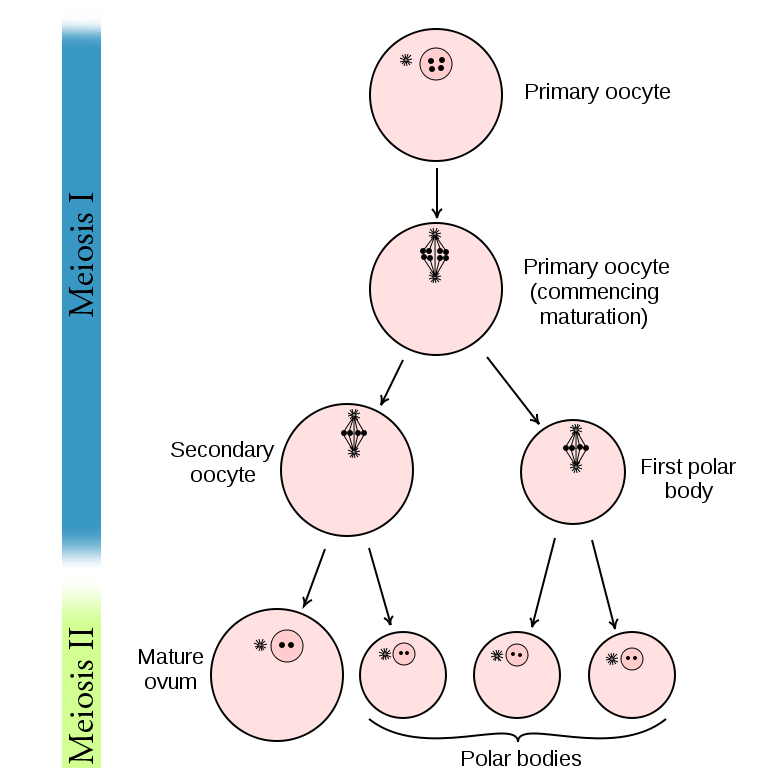
\includegraphics[width=0.800\linewidth]{oocyte-polar.png}
\caption{Asymmetric division of oocytes into polar bodies. The primary oocyte
asymmetrically divide into a secondary oocyte and a smaller polar body each
containing half the DNA of the mother cell. The secondary oocyte will
divide asymmetrically a second time to become the mature ovum while
expelling a polar body. This asymmetric division process allow the
formation of a large haploid cell. Adapted from Wikipedia – Gray's
Anatomy – and {\hyperref[index-latex:alberts2008]{{[}Alberts et al. 08{]}}}.}\label{index-latex:fig-asymetric-division}\end{figure}


\subsection{Cell Organelles}
\label{index-latex:cell-organelles}
Inside the cytoplasm, cells have a number of structures with different and
specialised functions which are called organelles. The position and state of
organelles is of great importance for the cell to achieve its functions.
Probably the most known organelle is the cell nucleus of eukariotic cells that
contains the genetic material. Attached to the nucleus is the endoplasmic
reticulum  which is the organelle responsible for translating
RNA coming from the nucleus to functional proteins that will be delivered
across the cell after maturation in vesicles. Theses vesicles are
transported across the cell both by dyneins and kinesins — molecular motors —
that walk along microtubules originating from the centriole part of the
centrosome but also by myosins walking along actin filaments.  All of those processes
consume energy in  the form of ATP, generated within the mitocondria spread
across the cytoplasm. A schematic of the cell with some organelles can be seen
on \hyperref[index-latex:albertcell]{figure  \ref*{index-latex:albertcell}}
\begin{figure}[htbp]
\centering
\capstart

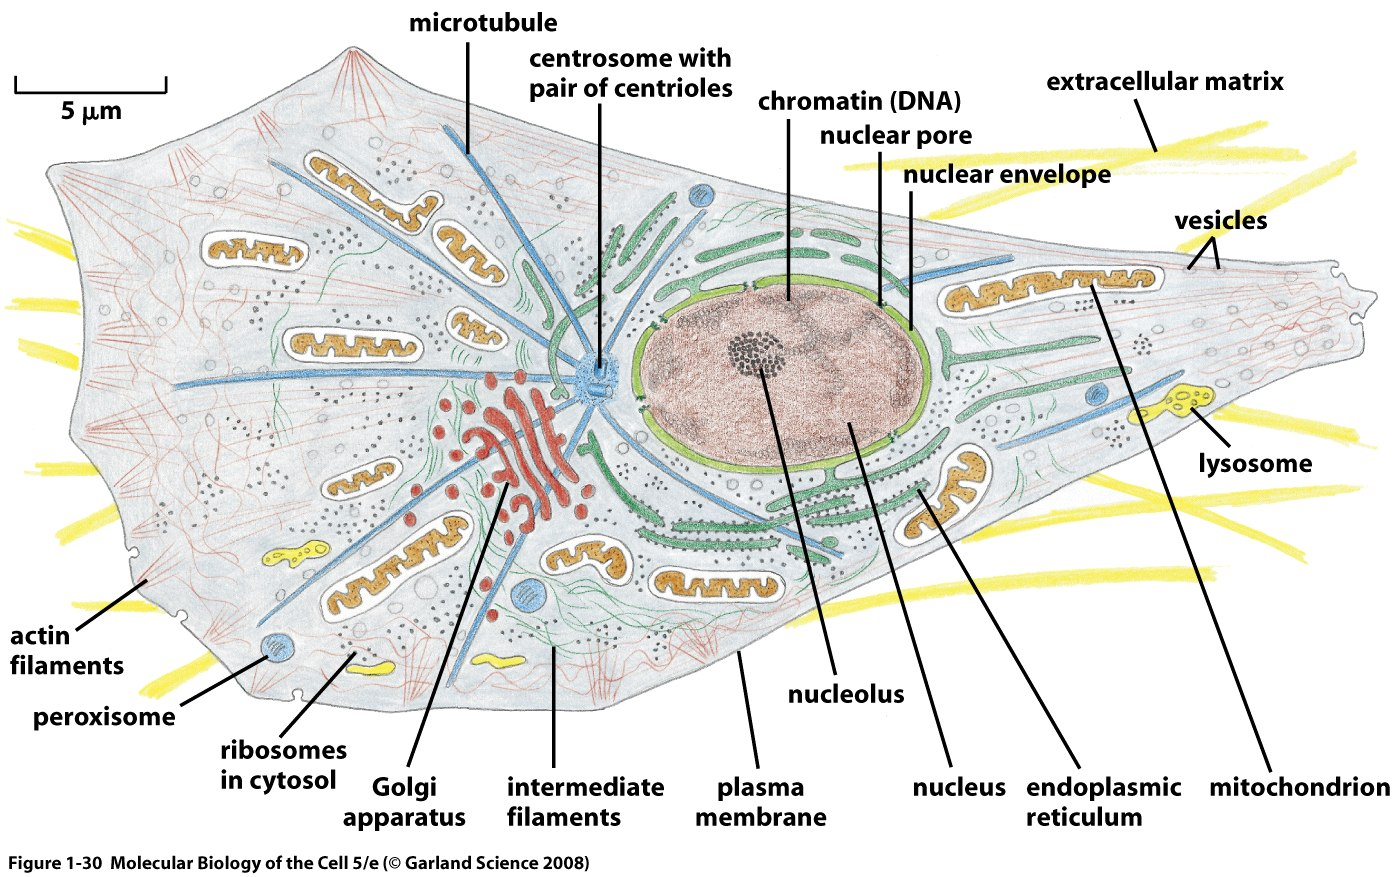
\includegraphics[width=0.800\linewidth]{figure-1-30.jpg}
\caption{Schematic of an eukariotic cell, adapted from {\hyperref[index-latex:alberts2008]{{[}Alberts et al. 08{]}}}. Visualized are
the many components that constitute the majority of cells.  Cell shape and
size can highly vary, from quasi spherical with a typical size of ten
micrometers to elongated neurones that can be tens of centimeters long.}\label{index-latex:albertcell}\end{figure}

The positioning of organelles is crucial for the life of the cell. During
meiotic division of cells, for example, it has been seen that the positioning of
the nucleus at the center of mouse oocytes happens before its
migration closer to the cortex to expel the first polar body. Failure to do so
results in a incorrect amount of DNA in germinal cell that can lead to
infertility.

It is already known that microtubules play a key role in organelle positioning.
Microtubules emanating from centrosome position at the two ends of the cell
during its division are used to fetch the correct chromosomes. Each
chromosome is pulled towards the centrosome which leads to each daughter
cell having the same amount of DNA.

Actin plays also an determinant role in organelle positioning process,
like in drosophila oocyte maturation where it positions the nurses cell away
from the dumping canal {\hyperref[index-latex:huelsmann2013]{{[}Huelsmann et al. 13{]}}}. In a later chapter ({\hyperref[index-latex:organelle-positioning]{\emph{Organelle
Positioning}}} (\autopageref*{index-latex:organelle-positioning})) we will develop a few keys points where
actin is indispensable in organelle positioning and how this relate to the
biomimetic actin networks we reconstitute.


\subsection{The Cytoskeleton}
\label{index-latex:intro-cyto}\label{index-latex:the-cytoskeleton}
The cytoskeleton, literally skeleton of the cell, is the structure which gives
the shape to a cell.  As for other multicellular animals that posses
skeleton, its shape is often a hint on how an organism moves. As feet, fins and
wings are characteristics that will tell you whether a animal
prefer land, see or air, the cytoskeleton will tell you many
things about a cell.

Unlike the (exo)-skeleton of animals which is rigid and
static, the cytoskeleton of cell is a  highly dynamic structure that keeps
remodeling itself on a short time scale compared to the speed at which a cells
move. Thanks to these dynamics, the cytoskeleton can achieve its
functions.  As vertebrates skeletons are necessary to transmit force from one part
of the body to another, the cytoskeleton is responsible not only to
transmit the forces the cell is exerting, but also to generate theses forces.
The cytoskeleton connect a cell to its environment,
both mechanically and biochemically.

We will consecrate a longer part of this work to describe the cytoskeleton.


\section{The Role And Composition Of The Cytoskeleton}
\label{index-latex:the-role-and-composition-of-the-cytoskeleton}\label{index-latex:role-of-actin}
We have already introduced the cell cytoskeleton in the previous part, and we will now
describe its components and functionality more in detail here.  The cytoskeleton
has three main functions, it connects the cell both physically
and biochemically to the external environment, generate and coordinate the
forces that give the cell its shape and allows it to move. It is also
responsible for organising spatially  the cell content {\hyperref[index-latex:fletcher2010]{{[}Fletcher et al. 10{]}}}.
The cytoskeleton is also in particular sensitive to spatial and temporal
information that can affect cell fate and the assembly of the cytoskeletal
structure. This can be seen for example with the bud scar of budding yeast that
persists after division.


\subsection{Composition of the cell cytoskeleton}
\label{index-latex:composition-of-the-cell-cytoskeleton}
The cytoskeleton is mainly composed of three types of filaments.
Microtubules, intermediate filament and actin filament, also known as
microfilaments.

Microtubules are the widest structure with a diameter of 20nm (\hyperref[index-latex:fig-mt]{Fig  \ref*{index-latex:fig-mt}})
and the
stiffest of the three kinds of filaments with a {\hyperref[index-latex:viscoelastic]{\emph{persistence length}}} (\autopageref*{index-latex:viscoelastic}) in the order
of millimeters, much longer than the size of the usual cell.
Microtubules are extensively studied {\hyperref[index-latex:valiron2001]{{[}Valiron et al. 01{]}}}.
Microtubules are formed by the polymerisation of a heterodimer of tubuline
that leads to the formation of polar (oriented) filaments that can be walked on
by molecular motors. These molecular motors can be decomposed in two families –
kinesins and dyneins – depending on the end towards which the motor preferably
walk.  Microtubules are mostly known for their action during mitosis
where they will form the majority of the mitotic spindle that drive the segregation
of the chromosomes in two groups, each group ending in one of the daughter
cells.

Microtubules have the characteristic of being highly dynamic by alternating
between two states of rapid growth and a rapid shrinkage. The transition from
microtubule growth to shrinkage is called a \emph{catastrophe}, the transition from
shrinkage to growth is called a \emph{rescue}.
\begin{figure}[htbp]
\centering
\capstart

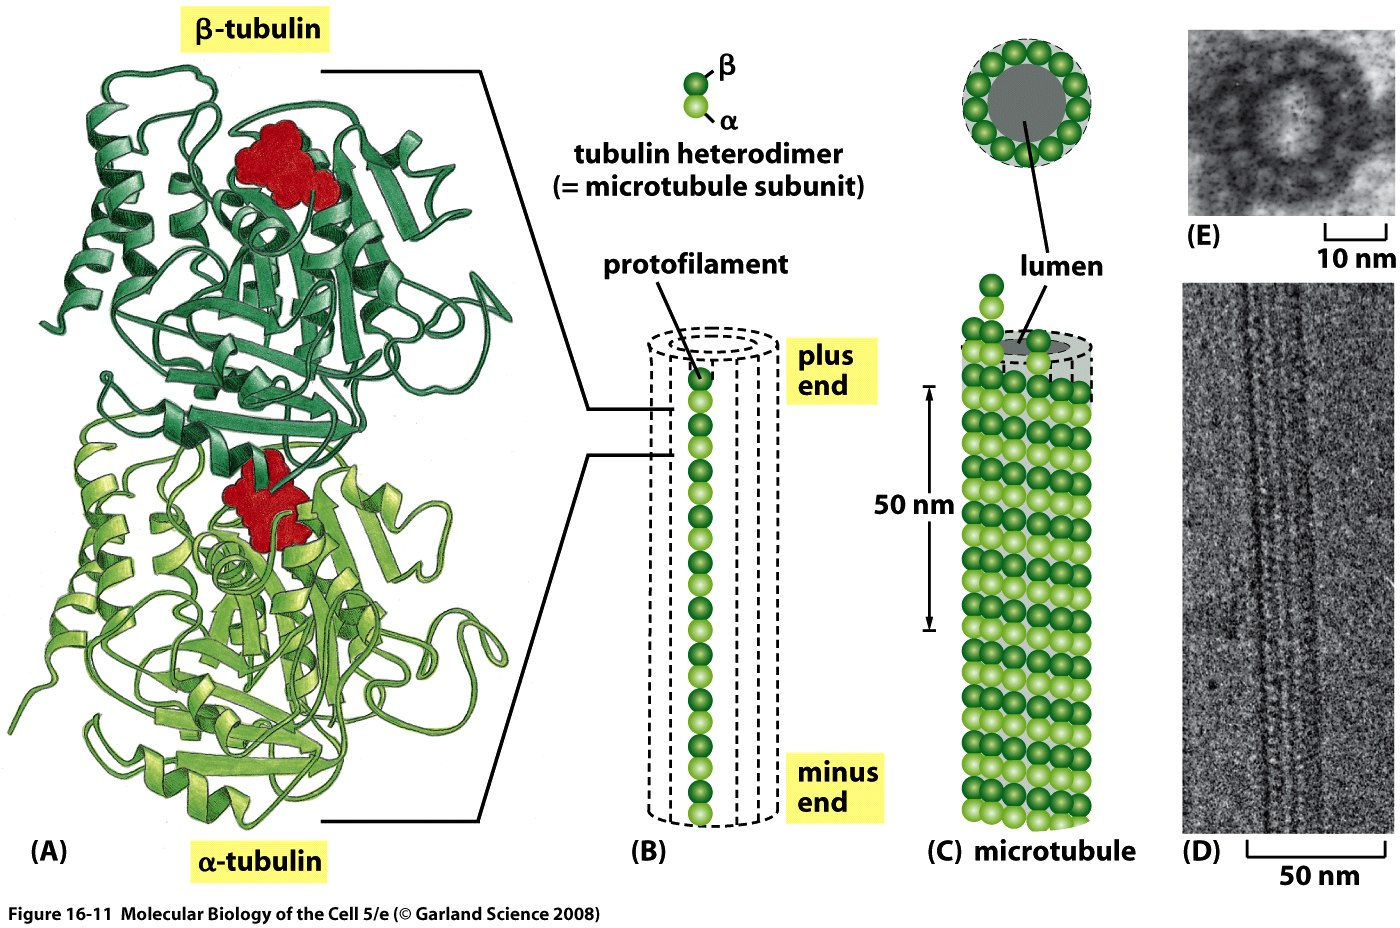
\includegraphics[width=0.700\linewidth]{microtubules-structure.jpg}
\caption{Structure of an heterodimer of tubuline and assembly into a microtubule.
Electron microscopy of a single microtubule filament. From {\hyperref[index-latex:alberts2008]{{[}Alberts et al. 08{]}}}.
A) Structure of heterodimer of tubuline B)
Heterodimers can assemble forming polar filaments. C) Filaments can
assemble into  microtubules. D,E) Electron microscopy image of
microtubules.}\label{index-latex:fig-mt}\end{figure}

Intermediate filaments are of medium diameter in the order of around 10nm, in
between actin and microtubules filaments, hence their name.  Unlike microtubules
and actin filaments, intermediate filaments are composed by several sub-families
of proteins and are non-polar.

Intermediate filament have an important role in the mechanical properties of
cells due to the fact that they are particularly  resistant to stretching.

Unlike actin and microtubules, they are thought to be passive, with mechanical
properties mainly deriving from how multiple filaments are linked together
laterally.

Actin, is the third component of the cytoskeleton, the one on which  we will
focus on most of our efforts. Actin monomers, also called \emph{G-Actin} for globular actin can polymerise.
By polymerizing actin monomers (G-actin) into actin filaments (\emph{F-actin}), the
thinest of the three cytoskeletal components forms. Actin is produced in the
cell as a globular protein of \textasciitilde{}40 kDa (\hyperref[index-latex:fig-actin]{Fig  \ref*{index-latex:fig-actin}}) that once associated with ATP or ADP
polymerises into helicoidal filament with a diameter between 7 and 9nm. The
formed actin filaments are polar, where both extremities are respectively called the
plus (\emph{+}) or barbed end, and the minus (\emph{-}) or pointed end. The polarity of
the actin filament is of importance as this gives rise to a preferred direction
for most processes that can happen on the filaments.

The actin protein is highly conserved across species, and is know to directly
interact with hundreds of proteins {\hyperref[index-latex:dosremedios2003]{{[}DosRemedios et al. 03{]}}}.

Single undecorated filaments will behave  as
semi-flexible polymers at the scale of the cell with a persistence length in the order of 10 µm {\hyperref[index-latex:isambert1995]{{[}Isambert et al. 95{]}}}. When they
assemble into different structures and networks, or associate with other proteins
and molecules the resulting mechanical and dynamic properties can be highly variable.
\begin{figure}[htbp]
\centering
\capstart

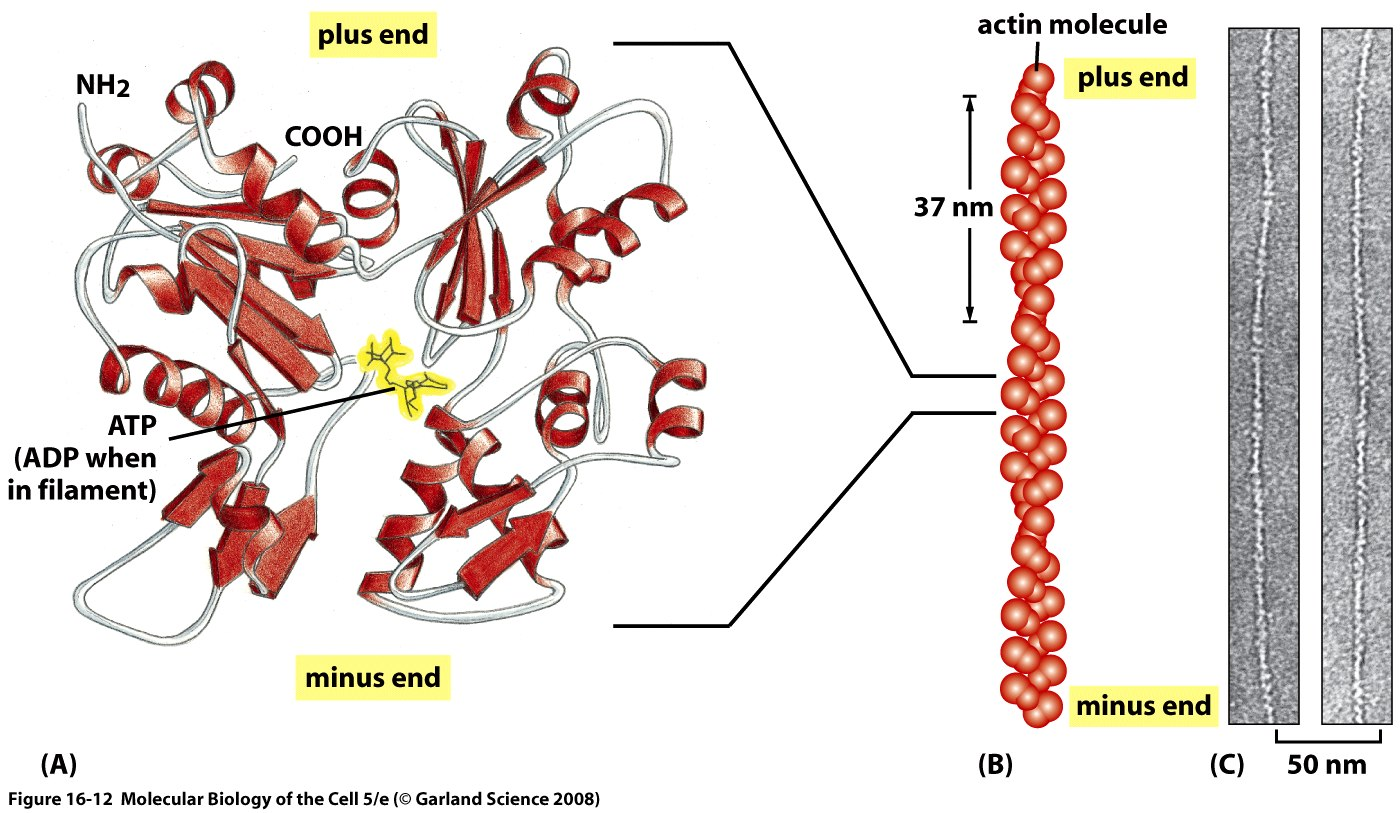
\includegraphics[width=0.700\linewidth]{actin-structure.jpg}
\caption{A) Structure of a single monomer of actin, and electron microscopy snapshot.
— from {\hyperref[index-latex:alberts2008]{{[}Alberts et al. 08{]}}}.}\label{index-latex:fig-actin}\end{figure}


\subsubsection{Dynamics of actin polymerisation}
\label{index-latex:dynamics-of-actin-polymerisation}
The assembly mechanisms that allow to go from single monomers of actin (also
refer to as G-actin for globular actin) to actin filament (also refer as
F-actin) need to be well understood to explain the different network
structures created by actin filaments in the presence of other proteins.

The polymerisation of ATP/ADP actin monomers to form an actin filament need to
go through the step of forming an actin proto-filament which is constituted of
at least 3 actin monomers. This will most of the time be the kinetically
limiting step. Once proto-filaments are present in solution, single monomers
can be freely added or removed on both ends of the filament.  The process of
forming these proto-filaments is called nucleation and it is the rate limiting
factor to form actin filaments. To circumvent this
limitation experimentally one can use preformed actin filament seeds, or actin nucleators
to direct the polymerisation on the cell.

We need to distinguish between the dynamics of polymerisation and
depolymerisation on both ends of the filament. Indeed, it has been show that the
association and dissociation rates are differ between the pointed (-) and
barbed (+) end. The barbed end has  higher dynamics than its pointed
counterpart which is the reason for its (+) name. The dynamics of
polymerisation is higher both in he case of ATP and ADP, though the rate
constant of association and dissociation differ for both kind of filaments (\hyperref[index-latex:fig-actin-pollard]{Figure  \ref*{index-latex:fig-actin-pollard}})
\begin{figure}[htbp]
\centering
\capstart

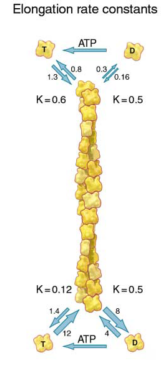
\includegraphics[width=0.250\linewidth]{elongation-rate-constant.png}
\caption{Association and dissociation rate of both ATP and ADP actin on pointed and
barbed end as measured in {\hyperref[index-latex:pollard1986]{{[}Pollard 86{]}}} (scheme from {\hyperref[index-latex:pollard2003]{{[}Pollard et al. 03{]}}}).
The difference of equilibrium constant between the barbed end (bottom)
and pointed end (top) in the presence of ATP allow filament treadmilling.}\label{index-latex:fig-actin-pollard}\end{figure}

The equations that drive the polymerisation can be written as follow
\phantomsection\label{index-latex:equation-roa1}\begin{gather}
\begin{split}\left. \frac{dn}{dt} \right|_{barbed} &= k_{+,{barbed}}.[GActin] - k_{-,{barbed}} \\
\left. \frac{dn}{dt} \right|_{pointed}&= k_{+,{pointed}}.[GActin]- k_{-,{pointed}} \\\end{split}\label{index-latex-roa1}
\end{gather}
Where \emph{barbed} and \emph{pointed} designate respectively the barbed and pointed end,
\(\left.\frac{dn}{dt} \right|_{barbed|pointed}\) represent the variation of
the number of actin monomers  which is due to addition or removal at the
barbed (respectively the pointed) end of actin filaments.  The association
rate constant \(k_+\) and dissociation rate constant \(k_-\) are the
polymerisation and de-polymerisation rate.  The concentration in barbed and
pointed-end denoted by \(C_{{barbed}/{pointed}}\) , \([GActin]\) is the
concentration of action monomers in solution. By assuming that the
concentration of pointed ends is equal to the concentration of barbed ends (no
capped or branch filaments), one can derive the steady state which give rise to
the critical monomer concentration below which an actin filament cannot grow:
\([GActin]_c\).

The rate constants of elongation of actin have been determined and depend on
whether the monomer is bound to ADP or ATP {\hyperref[index-latex:pollard1986]{{[}Pollard 86{]}}}. We should
consider the fact that the  ATP bound to actin will hydrolyse to ADP-Pi before releasing
the inorganic phosphate. The hydrolysis and phosphate release rates also depend on whether the
monomer is part of a filament or in solution. The hydrolysis of ATP-bound
actin into ADP bound actin in the filament  leads to an imbalance of actin
(de)-polymerisation on both ends. The actin filaments preferably
grow from the barbed end and shrink preferably from the pointed end.

This will lead to a phenomenon known as treadmilling where a single actin
monomer bound to an ATP molecule, will be incorporated at the \emph{+} end of the
filament and progressively migrate toward the \emph{-} end, eventually hydrolysing its
ATP into ADP before detaching from the filament on the pointed end. During this
process the filament will grow / shrink until it reaches the stationary state
where its length would stay constant but the treadmilling continues.

Treadmilling requires an imbalance in the global rate constant on the barbed and
pointed end and an energy source, in the case of actin this is provided by the
hydrolysis of ATP into ADP+Pi before releasing the inorganic phosphate, without
which treadmilling would not occur.

Practically, this can be approximated by having only ATP monomers at the barbed
end of actin filaments while the pointed end is typically constituted only of
ADP monomers, thus the critical concentration is lower at the  pointed end
compared to the barbed end. The growth speed of the filament on both
ends depends on the monomer concentration in solution. In between the
critical concentration of both ends, there exists a concentration at which the
polymerisation on (+) exactly compensates the depolymerisation on (-).


\subsubsection{Actin network can be controlled by a host of actin binding proteins}
\label{index-latex:actin-network-can-be-controlled-by-a-host-of-actin-binding-proteins}
Despite the already complex process of actin polymerisation and the
number of parameters that we have already introduced, the formation of an actin
network is an even more complex process that involves many other components.
Especially, actin monomers and filaments can interact with a high number of
proteins that will affect the previously introduced dynamics.  We will present
some categories of such proteins in the following.


\paragraph{Formins}
\label{index-latex:formins}
\emph{Formins} are polymerase proteins that will increase the polymerisation rate
of actin filaments by dimerizing and binding to the barbed end. It has the
particularity of being processive, meaning that it will stay bound to the
barbed end while catalysing the addition of new monomers. The processivity of
formins also permits the control of the localization of actin polymerisation
where formin proteins are present, like the tip of filopodia {\hyperref[index-latex:faix2006]{{[}Faix et al. 06{]}}}
{\hyperref[index-latex:bornschlogl2013]{{[}Bornschlogl 13{]}}}. \emph{Formins} posses domains rich in proline, capable of
binding to profilin (\emph{FH1}) which allows formin to elongate F-Actin using actin
monomers bounds to profilin {\hyperref[index-latex:pruyne2002]{{[}Pruyne et al. 02{]}}} {\hyperref[index-latex:pring2003a]{{[}Pring et al. 03{]}}}.


\paragraph{Capping Protein}
\label{index-latex:capping-protein}
To regulate polymerisation, cells also have the possibility to reduce or stop
the polymerisation. To achieve this, some proteins will bind to the growing end
of actin filaments and prevent the addition of new monomers.  \emph{Capping Protein}
(CP) being one particular example that will specifically bind to the barbed end
of a growing filament and  prevent it from growing. Capping proteins are
necessary to prevent polymerisation of actin in undesired area
and are essential for the structure and mechanical properties of actin gel
{\hyperref[index-latex:kawska2012]{{[}Kawska et al. 12{]}}}. \emph{Gelsoline} is another example of Capping Protein, that
unlike CP can only attached to the barbed end of an actin filament after
severing it. Gelsoline is hence both a severing and a Capping Protein.


\paragraph{Cross-linkers}
\label{index-latex:cross-linkers}
We have seen that some proteins were able to attach to actin filaments. When
such a protein is able to attach to many filament at once, it can act as an
attachment point between the two filament, preventing them to move with respect
one to each other. Such proteins, are referred to as cross-linkers.

The amount of freedom in movement between the two filaments depends on the
cross-linker used. For example , \(\alpha\)-actinin will allow rotation of the two
filament at their anchoring point whereas cross-linkers like fascine will prefer
a parallel conformation of the filament and favor the formation of actin
bundles.

Cross-linkers are essential for the formation of elastic network as they allow
forces to be carried from one actin filament to the other. The quantity of
cross link of a network will often be a key parameter for the elastic properties.
The distance between the link points in the network (both cross links
and entanglement points) will give the typical network mesh-size which is used
to calculate the viscoelastic response of networks : {\hyperref[index-latex:morse1998a]{{[}Morse 98a{]}}}.


\paragraph{Stabilizing actin filaments}
\label{index-latex:stabilizing-actin-filaments}
As actin networks are dynamic constructs that are changing shape and properties
over time, it is convenient to be able to stabilize those networks. Tropomyosins
are proteins capable to bind on the side of actin filament to stabilize them.

The use of phalloidin, a toxin extracted from fungus (Amanita phalloides), binds
between F-actin subunits on the filament, and hence  prevents it from
de-polymerising.  Though, it is known that stabilizing actin filaments with
phalloidin will increase their stiffness as measure by the persistence length which can change the
mechanical properties of the formed actin network.


\paragraph{Profilin}
\label{index-latex:profilin}
Profilin is a protein that will bind to the barbed end of single monomers of
actin in solution.  By doing so it will first prevent the association of
monomers into dimers and trimmers, thus preventing the nucleation of actin
filament. It thus allows a better control of localisation of actin filament
both in vivo and in vitro in the presence of actin seeds of actin nucleator.

Profilin was for a long time believed to be only a sequestering protein
that inhibit polymerisation {\hyperref[index-latex:yarmola2009]{{[}Yarmola et al. 09{]}}}, though it has a more complex
behavior, and if it prevent polymerisation of actin filaments by the pointed
end, it can facilitate polymerisation. One of the cause of increase in
polymerisation speed by profilin is the fact it binds preferably to ADP-Actin
and increase the exchange rate of ADP into ATP.


\paragraph{Branching Agent}
\label{index-latex:branching-agent}
A type of network found of the leading edge of cells lamellipodia is dendritic
network. It is characterised by tree-like structure of actin filaments in which
thanks to the Arp2/3 complex branching agent a mother actin filament will form a
daughter filament on its side.

We have seen previously that crosslinkers are proteins capable of linking two
or more actin filaments together by binding on their side. Another mechanism
involving binding on the side on actin filament is responsible for a closely
related network, the branching mechanism.

The Arp2/3 complex is composed of seven subunits, two of which are highly
similar to actin, forming the Arp2 and Arp3 family for Actin Related Proteins,
giving the complex its name. Typically Arp2/3 will bind on the side of a pre-existing
actin filament, hence initiating the growth of a daughter filament with an angle of
70° to the mother filament. The newly created daughter filament pointed end
is terminated by the Arp2/3 complex that will stay attached to the mother
filament, thus increasing the number of available barbed end, without changing
the number of available pointed end. See Nature Review by Erin D. Goley and
Matthew D. Welch {\hyperref[index-latex:goley2006]{{[}Goley et al. 06{]}}} for  a longer review about the Arp2/3
complex.

In cells, the Arp2/3 complex needs to be activated by a Nucleation Promoting
Factor (NFP).  Among them is the  WASp protein (Wiskott-Aldrich Syndrome
protein) and its neural homologue N-WASP which are from the same family as
SCAR/WAVE {\hyperref[index-latex:machesky1999]{{[}Machesky et al. 99{]}}}.  All these activators of Arp2/3 have in common a
WCA motif. The wild type protein need to be activated in order to activate Arp2/3.
The activation is done by a change in conformation that exposes the active
region and provides the first actin monomer necessary for nucleation of the
daughter filament (\hyperref[index-latex:fig-pwa-deploy]{Figure  \ref*{index-latex:fig-pwa-deploy}}).  To circumvent the activation process of
these proteins, we use a reconstructed version of the protein that cut all
region before the poly-proline. This confer to pVCA the ability to be
permanently active. This region can also be replaced by streptavidin in order
to selectively bind pVCA to selected regions. Characterisation and more
detailed description of pVCA can be found in {\hyperref[index-latex:noguera2012]{{[}Noguera 12{]}}}.
\begin{figure}[htbp]
\centering
\capstart

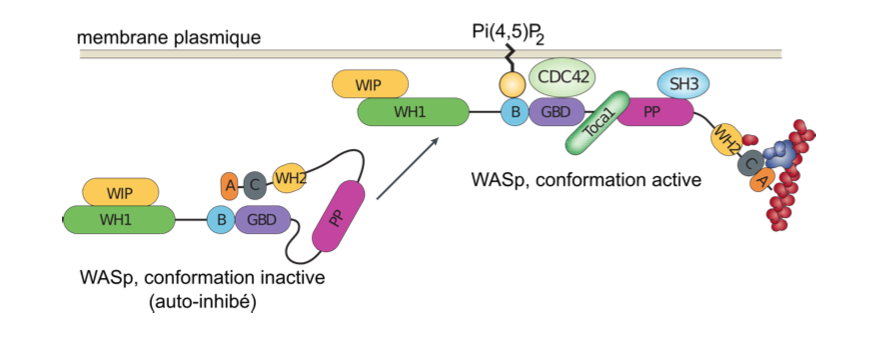
\includegraphics[width=0.600\linewidth]{pwa-deploy.png}
\caption{Organisation of Wasp domains. A change in conformation make the protein
active, which allow the activation of the Arp2/3 complex and the nucleation
of a daughter filament.  Adapted from {\hyperref[index-latex:goley2006]{{[}Goley et al. 06{]}}}}\label{index-latex:fig-pwa-deploy}\end{figure}

Unlike Cells that are able to control the localisation of actin nucleation
processes thanks to activation of WASp and its homologue, the `in vitro' control
of localisation of actin polymerisation is directly done by the localisation of
pVCA.

The network formed by Arp2/3 is called a dendritic network, and is in
particular found at the leading edge of the cell in the lamellipodia. It is
such a network that is present in the bead system we will study hereafter.

As for crosslinkers, dendritic networks are able to carry forces across single
actin filaments by the intermediary of Arp2/3. Two dendritic network of Arp2/3
can also entangle and allow forces to be carried across them
{\hyperref[index-latex:kawska2012]{{[}Kawska et al. 12{]}}}.
\begin{figure}[htbp]
\centering
\capstart

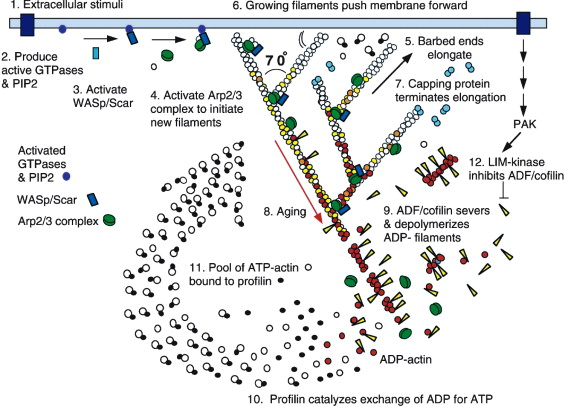
\includegraphics[width=0.700\linewidth]{pollard2003-actin-cycle.jpg}
\caption{Schematic recapitulating the formation of
a dendritic network at the leading edge of a cell were several of the
function of protein can be seen. An actin nucleation promoting factor
(Active WASp,  blue rectangle at the membrane) will activate Arp2/3 (green
blob) which will act both as nucleation factor and a branching agent. From
an activated Arp2/3 will grow an actin filament pointing towards the
membrane. Newly growing barbed ends, rich in ATP-actin (white circle) can
eventually be capped by Capping Protein (light-blue pairs of circle) which
will terminate their growth.  Aging monomers in actin filament will slowly
hydrolyse their ATP (yellow and red circle), eventually releasing the
inorganic phosphate before detaching from the pointed end.
Depolymerisation is helped by severing protein (sharp triangle) and Actin
Depolymerisation Factor (ADF). ADP-actin monomer will bind to profilin
(Black dots) increasing the turn over rate to ATP-actin which will be reused
by the leading edge of the cell. Adapted from {\hyperref[index-latex:pollard2000]{{[}Pollard et al. 00{]}}}.}\label{index-latex:actin-cycle}\end{figure}

A schematic that recapitulate the interaction of actin with other protein and
the formation of a dendritic network at the leading edge of the cell is
presented on \hyperref[index-latex:actin-cycle]{figure  \ref*{index-latex:actin-cycle}}.


\paragraph{Molecular Motor}
\label{index-latex:molecular-motor}
A particular kind of protein that can bind to the cytoskeletal filaments are
molecular motors. Molecular motors are proteins that will consume energy
in the form of ATP, hydrolyse it to change conformation and produce forces.

The motors that move along actin filaments are part of the myosin superfamily, they
are both responsible for the transport of cargo along filaments, cell motility,
division, and muscle contraction. They acquire their name from their discovery
in 1864 by Willy Kühne who extracted the first myosin II extract from muscle
cell {\hyperref[index-latex:hartman2012]{{[}Hartman et al. 12{]}}}.

The myosin super family is divided into subfamilies numbered with roman literals.
As of today we count more than 30 families of myosin {\hyperref[index-latex:berridge2012a]{{[}Berridge 12{]}}}.
Muscle myosin is part of the myosin II family and is often referred to  as
conventional myosin for historical reason as being the first discovered.
Non-muscle  myosin are also referred to as unconventional myosin.

Myosin motors seem to be shared among the living domain, hinting for an
early emerging of myosin in the evolution. All the myosin motors move on actin
filaments toward the barbed end, with the exception of myosin VI which moves
towards the pointed end {\hyperref[index-latex:buss2008]{{[}Buss et al. 08{]}}}.

Different subfamily of myosin are used for different function in cells. Even in
subfamilies each type of myosin can have specific functions. For example,
conventional myosin found in muscle cells are use for large scale cell
contraction. In contrast, myosin V is known to transport cargo and is found to
be responsible for actin network dynamics and vesicle positioning
{\hyperref[index-latex:holubcova2013]{{[}Holubcova et al. 13{]}}}.


\subparagraph{Myosin II}
\label{index-latex:myosin-ii}\label{index-latex:myoii}
As stated before, the myosin II family both encompass conventional myosin as
well as Non-muscle myosin II (NMII). Both have a similar structure (\hyperref[index-latex:fig-myosin]{Fig  \ref*{index-latex:fig-myosin}}).

All myosin IIs are dimers constituted of two heavy chains and light chains. The
heavy chains are held together by a coil-coiled alpha helix referred to as the
tail. On the other side of the protein sequence is a globular head, which is
responsible for ATP hydrolysis and is able to convert the energy from the
hydrolysis into mechanical force. It is also the part that will bind to the
actin filaments. In between the tail and head is the neck domain that acts as a
lever to transmit the force generated by the head to the tail. The length of
the neck influences the length of the movement done by the cargo at each step of
the myosin as well as the size of the step the myosin can effect. The two light
chains are situated in the neck region and are responsible for the myosin
activity regulation.

Myosin II dimers can align and assemble by the tail region, forming myosin
minifilaments. These minifilaments are bipolar, having numbers of myosin head
with the same orientation at each extremity.

In the myosin II family, conventional myosin and NMII differentiate by the
size of the minifilaments they form. Muscle myosin will form minifilaments
aggregating around 200 dimers, where NMII minifilaments will be composed  only
of 10 to 20 minifilaments. The other characteristic of unconventional myosin
with muscle myosin is the mode of activation. Conventional myosin activity is
regulated by the amount of \(Ca^{2+}\) available, which frees the actin filaments to let the myosin motor bind. However, its
counterparts are typically activated by the phosphorilation of the Myosin Light Chain (MLC).

Another parameter that discriminates muscle from non-cell myosin is their duty
ratio.  The duty ratio is define as the ratio of the time the myosin stays
attached to an actin filament over the typical time of a contraction cycle.
By noting \(\tau_{on}\) and \(\tau_{off}\) the time the myosin head
spent attached/detached from  the filament, the duty-ratio or duty-cycle can
be noted :
\phantomsection\label{index-latex:equation-roa2}\begin{gather}
\begin{split}r = \frac{\tau_{on}}{\tau_{on}+\tau_{off}}\end{split}\label{index-latex-roa2}
\end{gather}
We will see in the following that the duty-ratio might have an important effect
on the processivity of the myosin.

It should be noted that as minifilaments can attach to actin filaments on both
ends, they can also act as a bridge that holds two points close to each other,
though having the properties of crosslinkers.


\subparagraph{Myosin V}
\label{index-latex:myosin-v}
Myosin V is an unconventional myosin. Unlike myosin II it does not aggregate
into minifilaments.  Though, myosin V has a similar structure to myosin II but
with a longer neck, this confers to myosin V the ability to realize longer
steps on actin filaments. Indeed, the myosin V step size is of 36nm, which is close to the
twisting length of actin filaments. This allows myosin V motors to walk along
actin filament without having to rotate around it with the helix they form. At the end the tail domain
myosin V posses another globular domain capable of binding to its cargo, and
the variability of this region is what mostly define the difference between the
different type of myosin V.

Myosin V also has a high duty-ratio, this leads to dimers having almost always
one of the two head of the myosin to be bound to actin. It grants to the myosin
V the ability to walk in a processive manner toward the barbed end of
the actin filaments, both head successively binding 36 nm in front of the other
head.
\begin{figure}[htbp]
\centering
\capstart

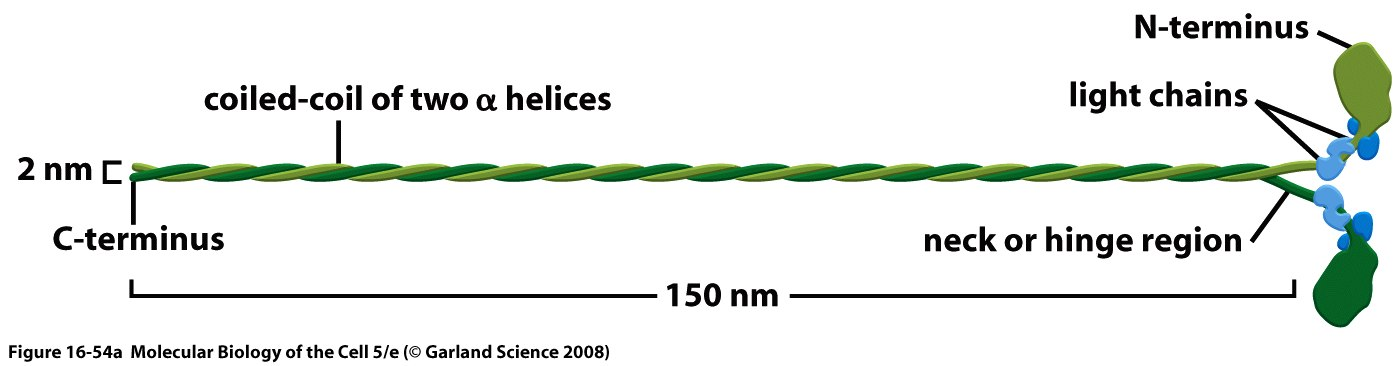
\includegraphics[width=0.700\linewidth]{figure-16-54a.jpg}
\caption{Schematic of a dimer of myosin motors with the example of Myosin II.
Each of the myosin monomer is colored in a
different shade of green. From Right to Left, the myosin head, with the N
terminal, is the part of the myosin that binds to the actin filaments. The
neck region with the light chain act as a lever arm. Finally the tail,
constituted with coiled-coil alpha-helix that aggregate to form minifilaments.
Adapted from {\hyperref[index-latex:alberts2008]{{[}Alberts et al. 08{]}}}.}\label{index-latex:fig-myosin}\end{figure}


\subparagraph{Myosin cycle}
\label{index-latex:myosin-cycle}
We saw earlier that the duty ratio of myosin was the ratio of time the head of
the myosin spent attached to the actin filament. Indeed, myosin can generate
displacement through a cycle of ATP hydrolysis and attachment/detachment
described below for a Myosin II motor:

The cycle can be decomposed in 5 steps, last of which will be responsible for
the forced exerted on the myosin cargo.
\begin{itemize}
\item {} 
The myosin start in the `rigor' conformation where it is lightly bound to
the actin filament.

\item {} 
An ATP molecule binds to the myosin head inducing the detachment of the
myosin from the actin filament.

\item {} 
ATP molecule is hydrolysed into ADP+Pi, providing energy which is stored
into a conformational change of the myosin which effects a recovery
stroke.

\item {} 
Inorganic phosphate is released as the myosin head attaches to the actin
filament.

\item {} 
The actin-bound myosin change conformation, applying forces on it's
cargo. This step is known as the power-stroke and is responsible for most
of the applied forces or displacements of the myosin. During the
power-stroke the ADP bound to the myosin head is released, leading back
to first step of the cycle.

\end{itemize}

This principle is the same for all kinds of myosins. In the case of Myosin II
the duty-ratio is only of about 5\%, which leave Myosin II detached from the
actin filament most of the time. A single dimer cannot achieve
processivity.   The tail of myosin II can bundle itself with the tail of other
myosin II motors.  They from large bipolar thick filaments of hundreds of dimers.
As each myosin dimer attaches and detaches independently from the actin
network the effective attachment of of the filament increases with the number
of motors in the minifilaments. Indeed the probability of having at least one
motor attached increases with the number of motors. The constant attachment of
at least one myosin II head in minifilaments insure that the filament does not
displace with respect to the actin network when others myosin heads recover
from their power stroke and reattach, thus conferring processivity to myosin II
minifilaments.

The bipolar nature of myosin II minifilaments also allow them to act as force
dipoles, each  of the extremity pulling the surrounding actin network or
filament towards the center of the minifilaments. This is the mechanism at the
origin of muscle contraction and can allow to build-up tension in actin network.


\subsection{The actin cortex}
\label{index-latex:the-actin-cortex}
The actin cortex is a thin layer of between 200 to 500 nm that can be found
just underneath the plasma membrane of a cell (\hyperref[index-latex:fig-electro-cortex]{Fig  \ref*{index-latex:fig-electro-cortex}}) . The properties of the actin
cortex makes it a key component to diverse processes.  Its capacity to resit
to, and transmit forces is indispensable for locomotion of many cells by
allowing the retraction of the rear of the migrating cell and will be describe
in more detail in the next section. Its structure is also essential for the
cellular division as contractility is necessary to generate cortical tension
and achieve the separation of the two daughter cells.

The actin cortex is constituted of actin filaments that can be parallel or
orthogonal to the membrane as one can see using electron microscopy on cells
{\hyperref[index-latex:morone2006b]{{[}Morone et al. 06{]}}}.
\begin{figure}[htbp]
\centering
\capstart

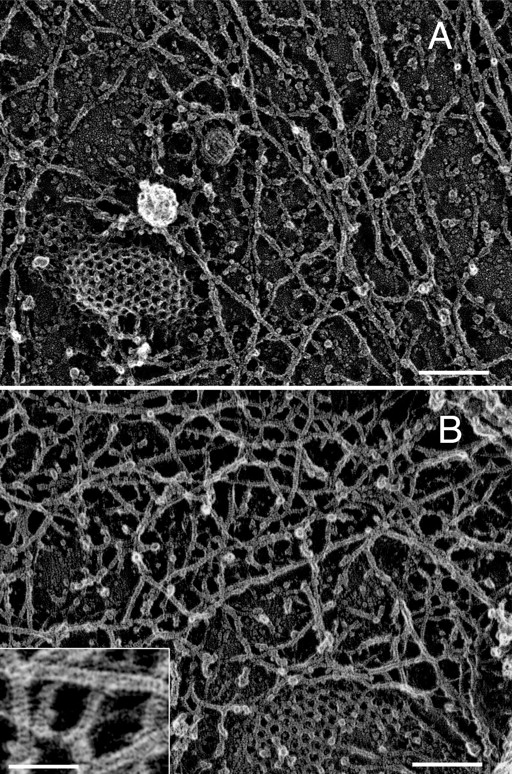
\includegraphics[width=0.700\linewidth]{Actin-Cortex-Moronne-2006.jpg}
\caption{Electron microscope view of the actin cortex in rat cell. The inset
show a periodicity of \textasciitilde{}5nm in filaments characteristic for actin.  Scale
bars are 100nm, inset 50 nm. Extracted from {\hyperref[index-latex:morone2006b]{{[}Morone et al. 06{]}}}.}\label{index-latex:fig-electro-cortex}\end{figure}

We saw through the bud scar of budding yeast that the full cytoskeleton could
retain memory of past events. It is also the case for simple actin networks as
show in {\hyperref[index-latex:parekh2005]{{[}Parekh et al. 05{]}}} who describe how actin-network growth can be
determined by network history, showing actin cortex could also act as a memory
for cell.


\subsection{Cell Motility}
\label{index-latex:cell-motility}
The way cells move highly depends on their environment and the cell type.
We can distinguish several strategies of movement, mainly categorised into
amoeboid and mesenchymal movement. The type of motility for certain
cells can be characteristic for malignant tissue, and plays a significant role in
the ability of the cells to invade nearby tissues.
\begin{figure}[htbp]
\centering
\capstart

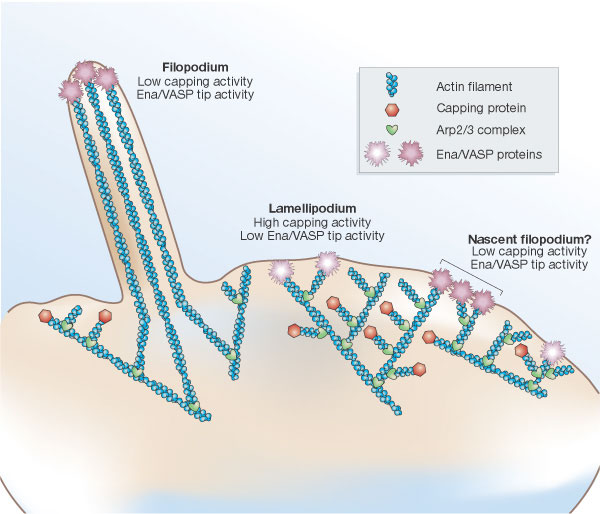
\includegraphics[width=0.600\linewidth]{Schafer2004.jpg}
\caption{Polymerisation at the leading edge of the cell. NPF situated on the
membrane of the cell localize the polymerisation. The lamellipodium will be
characterized by a dendritic network formed by Arp2/3. Parallel actin
structures can form a growing protrusion called filopodium.  Adapted form
{\hyperref[index-latex:schafer2004]{{[}Schafer 04{]}}}}\label{index-latex:fig-schafer}\end{figure}


\subsubsection{Lamellipodium based Motility}
\label{index-latex:lamellipodium-based-motility}
We can ave a first look into the mesenchymal mode of locomotion of cells, which is
also often referred to as crawling. To understand how a cell is able to crawl,
to move itself, we will in particular take the example of the lamellipodium.
The lamellipodium is a characteristic structure found in cells moving on a 2D substrate. By
its nature, motion using lamellipodia is one of the easiest to study using
microscopy which might explain why it is one of the best know process of cell
displacement. None the less, it does not diminish its importance in tissues
behavior as all epithelial cell can be considered as moving on a 2D substrate.
Beyond lamellipodia, further structures that are responsible for cell motion are
filopodia and pseudopodia. They mainly differ from lamellipodia by their shape
and the organisation of the actin structure inside (\hyperref[index-latex:fig-schafer]{Fig  \ref*{index-latex:fig-schafer}}). Lamellipodia-based motion
can move a cell up to a few micrometers per minute.

The action necessary to move in an mesenchymal way can be decomposed into three
steps. First the cell needs to grow a protrusion. Growing this protrusion is
typically governed by actin polymerisation just underneath the plasma membrane. The
lamellipodium is such a protrusion which is constituted by a 2D dendritic actin network
that polymerize at the leading edge. Second the cell's protrusion
need to attach to the surface. This is done through trans membrane proteins
that are bound to the actin cortex on the inside of the cell. The actin cortex
will act as a scaffold to transmit the force across the cellular to these
anchor points. The last part is the generation of traction in which the rest of the cell is pulled
toward the attached protrusion. The traction force is mediated through the
cytoskeleton and actin cortex while the contraction force themselves can origin
from actin network contraction and reorganisation due to myosin motors (\hyperref[index-latex:fig-lam-principle]{Fig  \ref*{index-latex:fig-lam-principle}}).
\begin{figure}[htbp]
\centering
\capstart

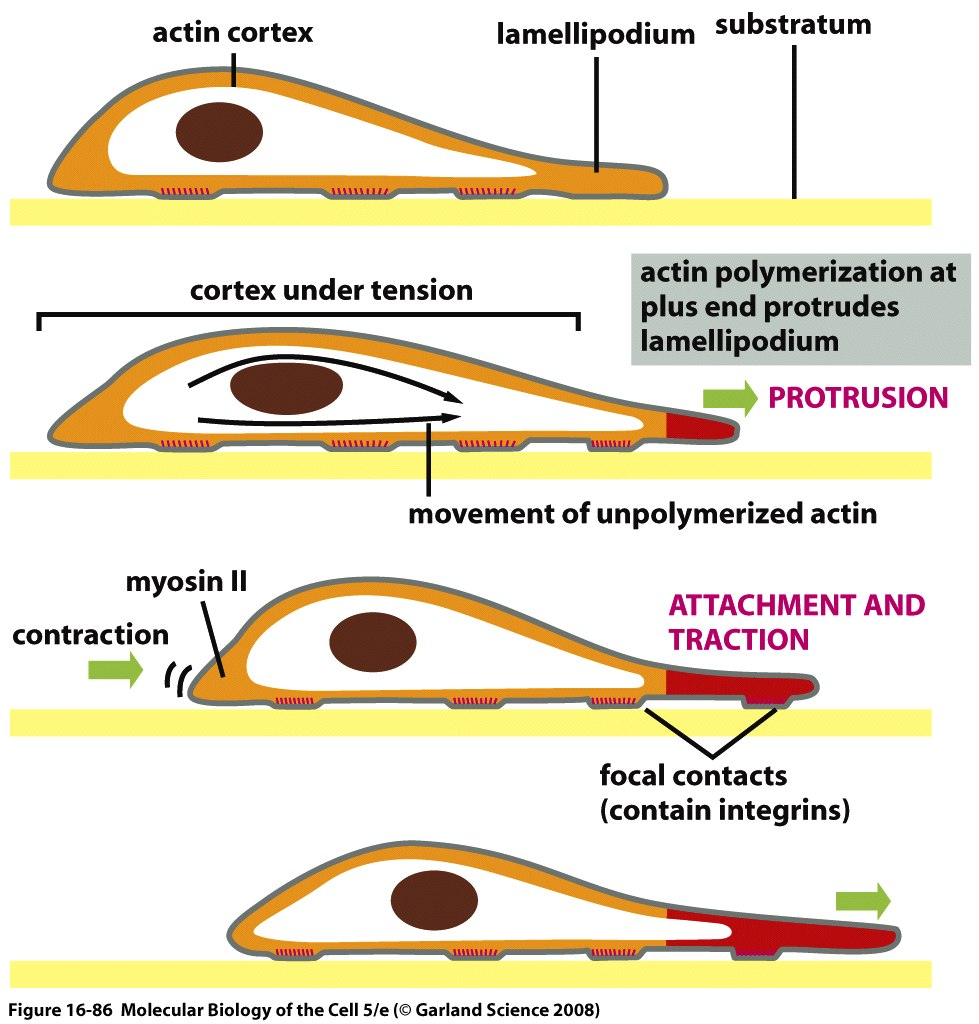
\includegraphics[width=0.900\linewidth]{figure-16-86.jpg}
\caption{Schematic of Lamellipodium base motility. The lamellipodium grows at the
leading edge of the cell and attach to a focal point. The actin cortex
under tension contract and is capable to pull the rear of the cell. Adapted
from {\hyperref[index-latex:alberts2008]{{[}Alberts et al. 08{]}}}.}\label{index-latex:fig-lam-principle}\end{figure}


\subsubsection{Blebbing based Motility}
\label{index-latex:blebbing-based-motility}
The second mode of motility which is known as amoeboid is more characteristic
of 3D displacement of cells. In this mode, the cell will also form protrusions
but will not rely on adhesion to move its body. This motility rely on blebs,
that are blister-like protrusion that appear on the cell surface. A bleb
forms on the surface of cell when the membrane detach from the actin
cytoskeleton underneath it, or when the cortex ruptures (\hyperref[index-latex:fig-bleb]{Fig  \ref*{index-latex:fig-bleb}}). The small protrusions
are formed, quickly grow as they lack the force supporting layer that the actin
cortex provides. While growing, the bleb fills with cytosol. The actin
cortex can rapidly reform on the bleb slowing down its growth. In some cases,
the reformation of the actin cortex in the bleb and the rebuilding of the
tension inside the bleb by myosins mediated contraction is enough to reverse
the bleb. Though, the content of the cell can also drain itself into the bleb
as it grows and while the main body of the cell contract and empties, thus
moving the cell from its old position to a new one in the direction of the
initial growth of the bleb.

At their initial state, blebs are simple membrane protrusions filled with
cytosol and empty of organelles. The stop of their growth is due to the
spontaneous formation of an actin cortex on the inner side of the bare
membrane.

By their relative simplicity to the rest of the cells, blebs are the perfect
system to be reconstituted \emph{in vitro} in liposomes.
\begin{figure}[htbp]
\centering
\capstart

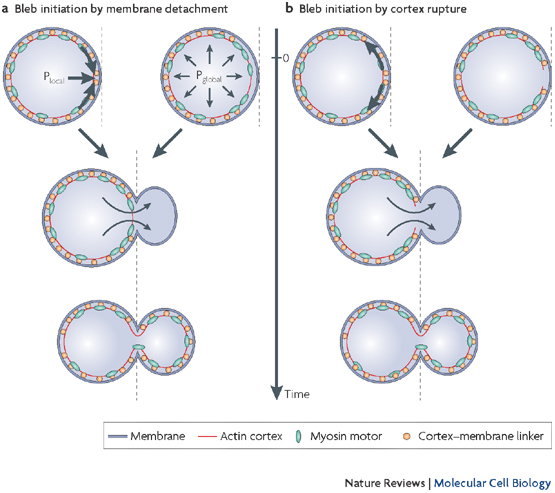
\includegraphics[width=0.400\linewidth]{Bleb-nature-paluch.jpg}
\caption{Formation of bleb can be done either by a) detachment of the membrane from
the cytoskeleton, or b) by a rupture of the cytoskeleton. In both cases the
inner pressure of the cell leads to the inflation of the membrane at the
point of rupture/detachment. The acto-myosin cortex will rapidly re-polymerize on
the inside of the bleb slowing down its growth until the expansion stops.
Extracted from {\hyperref[index-latex:charras2008]{{[}Charras et al. 08{]}}}}\label{index-latex:fig-bleb}\end{figure}


\subsection{Organelle Positioning}
\label{index-latex:id41}\label{index-latex:organelle-positioning}
We have seen previously that organelle positioning plays an important role in
cell function.  Several mechanisms involving actin are at the origin of
structure positioning in cells. The positioning of organelles by actin can have
a wide impact from being necessary for the correct cell division, to
allowing locust eyes to adapt in the dark by repositioning mitocondrion
{\hyperref[index-latex:sturmer1995]{{[}Sturmer et al. 95{]}}}.

We already know that the actin cortex is a necessary element in cell
motility. It also plays a determinant  role in organelle
positioning. It has been shown  {\hyperref[index-latex:chaigne2013a]{{[}Chaigne et al. 13{]}}} that the correct range
of elasticity of the actin cortex during oocyte division is needed for proper spindle
positioning. The correct spatial position of this spindle is necessary to
perform a viable division of the cell.

The actin cortex is not the only actin structure in the cell, beyond the thin and
dense layer just below the membrane lies a softer and sparser actin structure that has a
crucial role in organelle positioning.

During cell division, there are several stages that require actin structures.
As shown previously {\hyperref[index-latex:azoury2011]{{[}Azoury et al. 11{]}}} the expulsion of polar body during
oocyte asymmetric division is  strongly dependent on the time evolution of a
sparse actin network that can be found in the cell. Actin structures are  also
required at a later stage to permit the correct capture of chromosomes by
microtubules and achieve correct haploid division.  {\hyperref[index-latex:schuh2008]{{[}Schuh et al. 08{]}}} also shows
that a similar sparse actin network contracted by myosins is necessary for
spindle migration.

Especially in oocyte that are typically large, the effect of gravity is not
negligible. The presence of a sparse ``actin scaffold'' is discussed in
{\hyperref[index-latex:feric2013]{{[}Feric et al. 13{]}}}, where it is found that an actin network is present to
balance the gravitational force.

In drosophila, nurses cell need to expel their content into oocytes. It has been
observed {\hyperref[index-latex:huelsmann2013]{{[}Huelsmann et al. 13{]}}} that during this phase, the nurse cells' nucleus
is pushed away from the dumping canal by single actin filaments polymerising
from the membrane and forming a soft and sparse actin network.


\section{In vitro reconstituted actin networks}
\label{index-latex:in-vitro-reconstituted-actin-networks}
Living cells are complex organisms, for which each function requires a number
of interacting proteins and components. To understand the action of each
individual component, it is necessary to isolate or modify their actions
independently.

In order to achieve the precise tuning of each component independently, two
approaches are possible. First, an approach referred to  as ``Top-Down'', where
starting from the full system — in our case the cell — we will modify or remove
single or multiple components and study the global change of behavior. This is a complex
process that might be difficult to interpret, as biological systems often have
multiple pathways and feedback loops to regulate each of their processes. Taking into account the
large number of components that constitute a living cell, it is also
difficult to come up with the minimal system required to replicate certain behaviors.

The other approach, also referred to as the bottom-up approach, requires
the reconstitution of the system part by part until it replicates the expected
behavior. This is also a complex process, as there is a large number of potential components
likely to be added to the reconstituted system. This vast complexity
often leads to a wide range of testable parameters.
These controlled systems allow in principle for a deeper understanding of the governing
working mechanisms, and often permit access to a wider range of accessible
conditions and individual tweaking of components.

In our lab, we are mainly interested in the bottom-up approach and the use of
biomimetic systems. We try to reconstitute biologically relevant behavior within
minimal systems,  constituted from pure protein components.

I       n this manuscript in particular, we focus on mimicking the motility process
by which the \emph{listeria} pathogen is able to hijack cellular mechanisms, by recruiting proteins
responsible for actin polymerisation at the leading edge of the cell, and use
them to polymerize actin on the pathogen surface. This is what allows `listeria' to
propel itself fast enough (1.5 to 2 µm /min) {\hyperref[index-latex:dabiri1990]{{[}Dabiri et al. 90{]}}} to be able to
penetrate the cell membrane to move from one cell to the other.

The bead motility system is a minimal \emph{in-vitro} system capable of replicating
the listeria motility.


\subsection{Bead motility assay}
\label{index-latex:id49}\label{index-latex:bead-motility-assay}
The \emph{Listeria} pathogen is a 1.5 to 5 micrometer cylindrical bacteria that
enters cells, hijacks its actin polymerisation machinery to propel itself and
infect neighbour cells. It does so by the recruitment of a single protein on its
surface : ActA, that activates the Arp2/3 complex. By the recruitment of Arp2/3, a
dense branched and entangled actin network grows that will eventually form a
comet behind the bacteria propelling it at the speed of actin comet
polymerisation. Listeria comets are composed of a wide range of proteins. It has
been shown {\hyperref[index-latex:loisel1999]{{[}Loisel et al. 99{]}}} that the number of required components can
be highly reduced, still maintaining the motility features.

A simpler system replicating the listeria motility is the bead motility assay.
Consisting of a micrometer-sized bead covered with a nucleation promoting factor (NPF), it will activate the Arp2/3, present in the solution.

In the case of listeria, this NPF can be ActA, but such other NPF such as N-WASp or pVCA can also be used.
We chose pVCA in the experiments presented in this work. The NPF covered
bead is mixed with a G-Actin solution. Capping Protein is added to prevent
polymerisation from happening away from the bead surface as well as the
components required for actin polymerisation (ATP, Salt..., see {\hyperref[index-latex:m-et-m]{\emph{Material and methods}}} (\autopageref*{index-latex:m-et-m}))

Due to the presence of Capping Protein in the solution and NPF on the surface of
the bead, the polymerisation of actin will only happen
on the bead surface, forming a thin and dense actin gel capable of sustaining stress, depending
on the different protein concentrations. Unlike listeria, which
seems to control on which of its sides the nucleation process happens, this is not
controlled in bead motility assays. In the right condition, though,
{\hyperref[index-latex:kawska2012]{{[}Kawska et al. 12{]}}} the dense actin gel formed on the bead surface can
accumulate the stress induced by the inner layer polymerisation, until symmetry
breaking occurs. The gel ruptures on one side of the bead, leading to
the formation of a comet on the opposite side (\hyperref[index-latex:fig-bead-motility]{Figure  \ref*{index-latex:fig-bead-motility}}).
\begin{figure}[htbp]
\centering
\capstart

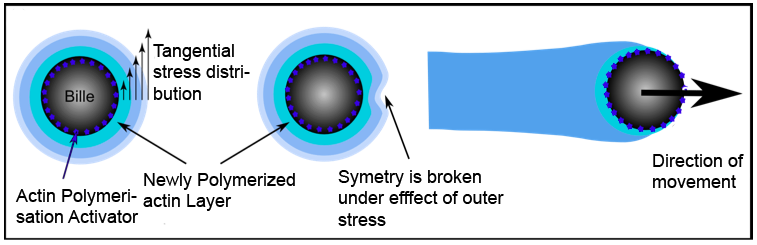
\includegraphics[width=0.600\linewidth]{Plastino-Sykes-2005.png}
\caption{Scheme of bead motility assay. The NPF (yellow stars) will localize the
actin polymerisation on the surface of the bead, thus increasing the stress on
the outer actin layer. At a sufficient level of stress, the outer layer
ruptures, leading to symmetry breaking, formation of a comet, and
propulsion of the bead. Adapted from {\hyperref[index-latex:plastino2005]{{[}Plastino et al. 05{]}}}}\label{index-latex:fig-bead-motility}\end{figure}

Due to the further polymerisation of the actin network on the surface of the bead,
the comet will grow, propelling the bead forward. This is the reason why the bead
system is a biomimetic system replicating the listeria motion.

It should be noted that during the movement of this system, two phases can be
distinguished. In the first phase, the system presents a spherical symmetry with
an homogeneous actin  network around the bead. The gel is growing from the
surface and is accumulating stress, due to the polymerisation of inner layers.

If the gel has accumulated sufficient stress by polymerisation,  the symmetry breaking event happens, and the system enters into
a second phase with the formation of a comet.

The conditions that lead to symmetry breaking have been investigated in detail
{\hyperref[index-latex:kawska2012]{{[}Kawska et al. 12{]}}}. In the absence of Capping Protein, the actin polymerisation
does not seem to be restricted enough near the surface of the bead, and thus the formed
network is not able to generate or sustain enough stress to achieve symmetry
breaking. At high Capping Protein concentration, the growth of the gel is heavily impaired,
thus preventing symmetry breaking. The concentration of Arp2/3 is also critical,
as Arp2/3 forms branched networks, and these branched networks are primordial essential for the
ability to sustain stress.
\begin{figure}[htbp]
\centering
\capstart

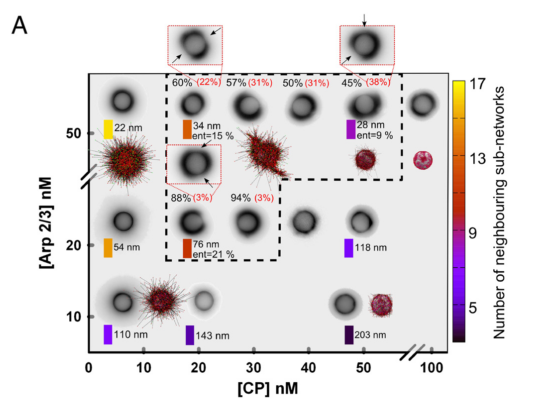
\includegraphics[width=0.700\linewidth]{symmetry-breaking-phase-diagram.png}
\caption{Phase diagram showing symmetry breaking in bead motility assay as a
function of concentration of Arp2/3 and Capping Protein. Symmetry breaking
only occurs inside the area delimited by the dashed line on 4.5 µm beads, both
\emph{in vitro} and \emph{in silico}. Experiments are
displayed as inverted fluorescence image. Adapted from {\hyperref[index-latex:kawska2012]{{[}Kawska et al. 12{]}}}}\label{index-latex:phase-diag}\end{figure}

In the rest of this chapter, we use the bead motility system, but only
consider it during the first phase, where the symmetry breaking has not yet
occurred, or in condition where it should not occur. In particular, we will
investigate a condition at 25 nM Arp2/3 with a concentration of Capping Protein
varying from 0 to 50 nM. As shown in \hyperref[index-latex:phase-diag]{fig  \ref*{index-latex:phase-diag}} this range corresponds to
conditions where no symmetry breaking occurs, but also to conditions in which
symmetry breaking is expected.  It should be noted that unlike
other studies that also characterize actin network growing on beads
{\hyperref[index-latex:pujol2012]{{[}Pujol et al. 12{]}}}, our system is still dynamically polymerising and thus
changing with time.


\subsection{Liposomes}
\label{index-latex:liposomes}
Beads are used as a model biomimetic system that replicates the polymerisation mechanism
happening on the leading edge of cells. Because of their composition and
rigidity, the phenomenon observed on beads cannot necessarily reproduce all the interactions and
processes that take place on the cell membrane. Cells are finite compartments with a
limited amount of actin that acts on the dynamics of polymerisation.  The fact
that cell size is in the order of the persistence length of actin filaments
also plays a role on the structure of actin networks. Indeed, at these scales, a
single filament can never reach the length at which it can be considered fully
flexible.

Liposomes are one of the biomimetic systems able to capture some
interactions between cell membranes. Liposomes are lipid bilayers that imprison
an aqueous compartment and exhibit many characteristics similar to cells.
The inside of liposomes can act as a biochemical reactor of limited size, with
the lipid bilayer acting as a separation from the outside, like the cell
membrane. The composition of the lipid layer can be varied in order to reflect
the composition of a cell membrane. In particular, it is possible to attach
proteins to the liposome membrane. Finally, the size of the liposomes can be
varied, leading to actin networks, the size and shape of which are similar to those found in
cells.

It is possible to mimic the cellular actin cortex using liposomes, and especially
its contractility. A crosslinked actin network can be formed and attached to
the outer leaflet of liposomes, and contractility can be triggered by injecting
molecular motors. The behavior of the system will depend on the attachment
between the reconstituted actin cortex and the liposome membrane.  A weak attachment
leads to a favorable rupture of the actin cortex during the increase of tension,
implying a symmetry breaking, as in the bead motility system.  In the case of strong
attachment, the liposome actin-cortex will accumulate tension until it has
enough force to crush the supporting lipid layer, thus collapsing the liposome
{\hyperref[index-latex:carvalho2013]{{[}Carvalho et al. 13b{]}}},(\hyperref[index-latex:fig-peeling-scheme]{Figure  \ref*{index-latex:fig-peeling-scheme}}). This system also allows the observation
over time, giving extra insight into the dynamics of the actin network (\hyperref[index-latex:fig-peeling-3d]{Figure  \ref*{index-latex:fig-peeling-3d}}).
\begin{figure}[htbp]
\centering
\capstart

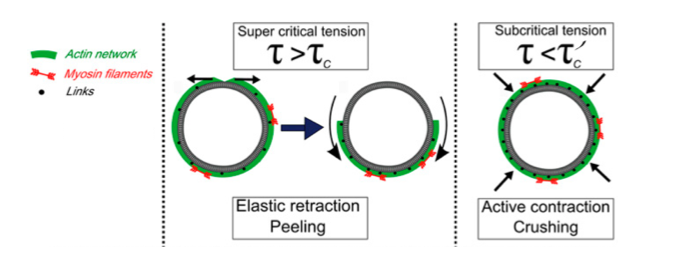
\includegraphics[width=0.800\linewidth]{joel-2-11.png}
\caption{Effect of reconstituted rigid actin cortex attachment to a liposome
membrane under constraints generated by myosin filaments. Under weak attachment,
the actin network ruptures thus leading to a ``peeling'' of the actin cortex.
With stronger attachment, the actin cortex can sustain higher stresses, until
the underlying liposome ruptures (``Crushing''). Adapted from
{\hyperref[index-latex:carvalho2013]{{[}Carvalho et al. 13b{]}}}}\label{index-latex:fig-peeling-scheme}\end{figure}
\begin{figure}[htbp]
\centering
\capstart

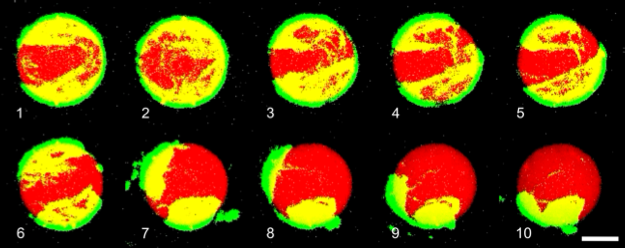
\includegraphics[width=0.900\linewidth]{joel-5-12.png}
\caption{3D reconstruction of an acto-myosin cortex (green actin) peeling off a
liposome (red) over time (1.4 second between frames). The actin cortex
contraction happened after the injection of Myosin II. Scale bar is 5 µm.
Experiments and reconstruction done by Joël Lemière.}\label{index-latex:fig-peeling-3d}\end{figure}


\section{Membrane Physics}
\label{index-latex:membrane-physics}
The cell's plasma membrane is a biological membrane that separates the cell from
its outside environment.  It consists of a lipid bilayer containing
a high number of proteins.  A lipid bilayer is formed by two layers of lipids and has a
thickness of a few nm. The classical theoretical description
of these bilayers has been done by W. Helfrich {\hyperref[index-latex:helfrich]{{[}Helfrich 73{]}}} in 1973 in a
model based on the elasticity and fluidity of lipid bilayers as well as the
self assembly properties of  lipids.

In the case of a close lipid bilayer, the potential energy stored by the
deformation of a lipid bilayer by unit area can be  written as
\phantomsection\label{index-latex:equation-eqa1}\begin{gather}
\begin{split}H = H_{ext} + H_{curv}\end{split}\label{index-latex-eqa1}
\end{gather}
In which \(H_{ext}\) is due to the extension/compression of the membrane,
and \(H_{curv}\) is due to the local curvature of the membrane.

The density of energy cost to extend the membrane \(H_{ext}\) can be written as a
function  of the elastic area compressibility modulus \(K_a\) and the
relative variation surface of the membrane \(A\) :
\phantomsection\label{index-latex:equation-eqa2}\begin{gather}
\begin{split}H_{ext} = \frac 1 2 K_a \left(\frac{\Delta A}{A}\right)^2\end{split}\label{index-latex-eqa2}
\end{gather}
\(K_a\) expresses how much energy is required to expand the surface of the
lipid bilayer and is due to the exposition of more hydrophobic surface to water
when expanding it. \(K_a\) is expressed in \(J.m^{-2}\), or \(N/m\)
and is close to twice the surface tension between the lipids and water.

For closed lipid bilayers, the total curvature energy can be expressed as the
sum of the curvature energy \(H_{curv}\) :
\phantomsection\label{index-latex:equation-eqa3}\begin{gather}
\begin{split}H_{cur} = \frac 1 2 \kappa (c_1 + c_2 -c_0)^2\end{split}\label{index-latex-eqa3}
\end{gather}
In which \(kappa\) is the bending modulus of the membrane and \(c_1,c_2\)
are the principal curvatures of the membrane. \(c_0\) is the spontaneous
curvature of the membrane, which is defined as the curvature the membrane would adopt, when free of
external constraints.

An important parameter introduced in membrane mechanics is the  membrane tension,
\(\sigma\) which is the stress associated with an increase in the membrane surface.
The tension \(\sigma\) is linked to the energy required to expand the membrane \(H_{ext}\) by :
\phantomsection\label{index-latex:equation-eqa4}\begin{gather}
\begin{split}\sigma &= \frac {\partial H} {\partial \left(\frac{\Delta A}{A}\right)} \\\end{split}\label{index-latex-eqa4}
\end{gather}
i.e.
\phantomsection\label{index-latex:equation-eqa5}\begin{gather}
\begin{split}H_{ext} &= \sigma\left( \frac {\Delta A} A \right)\end{split}\label{index-latex-eqa5}
\end{gather}
In which
\phantomsection\label{index-latex:equation-eqa6a}\begin{gather}
\begin{split}\sigma =  K_a \left( \frac {\Delta A} A \right)\end{split}\label{index-latex-eqa6a}
\end{gather}
Membrane tension is a key parameter as it can be measured in cells. It is one
of the parameters responsible for cell sorting {\hyperref[index-latex:maitre2012]{{[}Maitre et al. 12{]}}}. In particular
between cells, the tension of the couple (membrane+actin cortex) can be
determined by using the contact angle between cells which is the angle between
interfaces, as defined in \hyperref[index-latex:fig-tension-cell]{figure  \ref*{index-latex:fig-tension-cell}}.
\begin{figure}[htbp]
\centering
\capstart

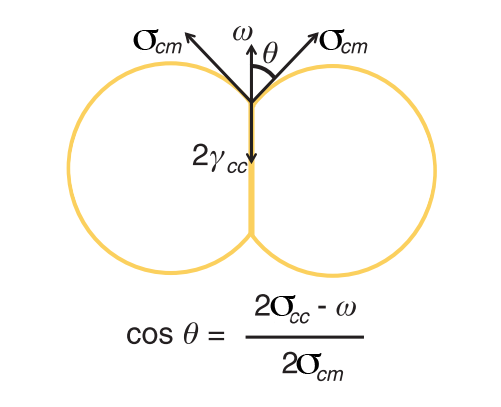
\includegraphics[width=0.400\linewidth]{Cell-Surface-tension.png}
\caption{Surface tension governs doublet shape,  adapted from {\hyperref[index-latex:maitre2012]{{[}Maitre et al. 12{]}}}.
The equilibrium of forces on the contact line governs the angle of contact
\(2.\theta\). \(\omega\) corresponds to the adhesion tension between
the two cells, \(\sigma_{cm}\) corresponds  to the tension between
the cell and the medium, \(\sigma_{cc}\) corresponds to the cortex
tension between the two cells.}\label{index-latex:fig-tension-cell}\end{figure}

In a later part, we use a reconstituted biomimetic system made of liposomes. The
injection of myosin motors changes the tension of the acto-myosin cortex
attached to a membrane. By determining the geometrical parameters of this
system, and in particular the evolution of the contact angle with time, we are
able to measure the variation of tension of the acto-myosin cortex due to the contraction by
molecular motors.


\section{Actin networks as viscoelastic material}
\label{index-latex:actin-networks-as-viscoelastic-material}\label{index-latex:viscoelastic}
We have previously seen that while polymerising, G-actin assembles into F-actin
filaments. The stiffness of filaments can be measured by a characteristic number
called the persistence length (\(l_p\)). More precisely, the
persistence length characterizes the average loss of correlation between the
tangents along the considered polymer. With \(s\) the curvilinear abscissae along the polymer,
and \(\Theta_{(x,y)}\) the angle between the two tangents at two different abscissae (\hyperref[index-latex:fig-persistence-length]{Figure  \ref*{index-latex:fig-persistence-length}}):
\phantomsection\label{index-latex:equation-eqa6}\begin{gather}
\begin{split}\left<\Theta_{(s,s+l)}\right> = exp\left(\frac{-l}{l_p}\right)\end{split}\label{index-latex-eqa6}
\end{gather}
For actin filaments, the
persistence length is in the order of 10 µm {\hyperref[index-latex:isambert1995]{{[}Isambert et al. 95{]}}}. This means
that for much smaller scales, the actin filament can be considered as rigid.
This is the case in the cell cortex where the meshwork has a typical size, smaller than 250 nm. In
the other extreme, at length scale much bigger than \(l_p\), filaments can
be considered as flexible. While in typical cells, the filament length is
rarely much bigger than the persistence length of actin, \emph{Xenopus} eggs can be
reach 1 mm, so hundreds fold the actin persistence length.
Still, for the majority of cells, the typical size we are interested in
is about the persistence length of an actin filament, thus at this scale, the filament can neither be considered purely
rigid nor completely flexible.
\begin{figure}[htbp]
\centering
\capstart

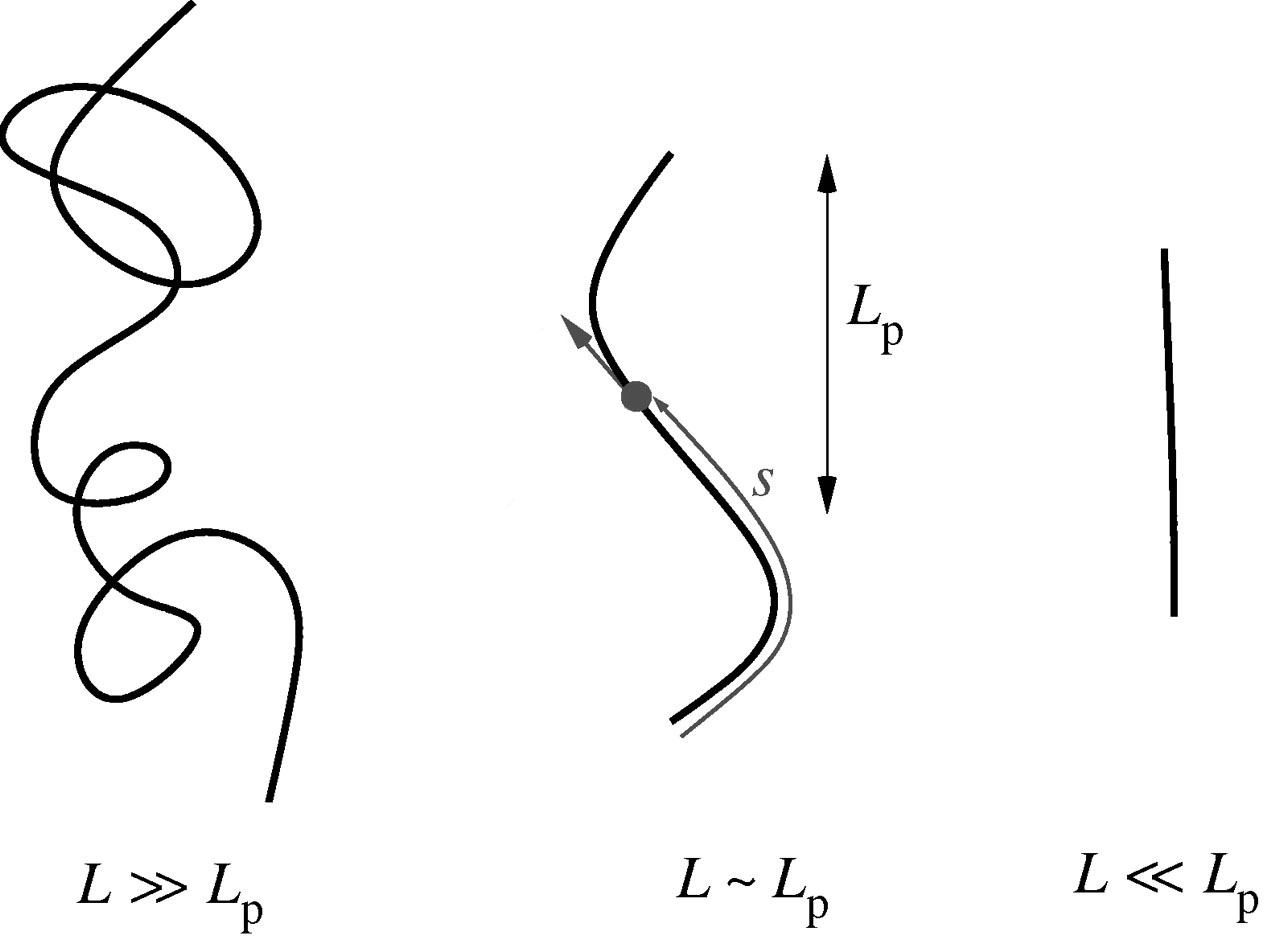
\includegraphics[width=0.600\linewidth]{F2_large.jpg}
\caption{Schematic of polymers with respectively big length compared to the persistence
length (A), in the order of the persistence length (B) and small compared
to persistence length (C), \(s\) as defined on (B) is the \emph{curvilinear
abscissae}, that is to say the distance between two points of the polymer,
measured by ``following'' the polymer. Adapted from {\hyperref[index-latex:liverpool2006]{{[}Liverpool 06{]}}}}\label{index-latex:fig-persistence-length}\end{figure}

For the above reasons, actin solutions are often compared to semi-flexible
polymers, and models that predict the behavior of actin networks often take
foundation on polymers physics {\hyperref[index-latex:morse1998b]{{[}Morse 98b{]}}} {\hyperref[index-latex:morse1998a]{{[}Morse 98a{]}}}. Still, if
these models rely on local microscopic parameters, experimental methods only
have access to bulk properties of the studied material, and it is from these
properties, and through the models, that we can deduce possible values for the
microscopic models {\hyperref[index-latex:mackintosh1995]{{[}MacKintosh et al. 95{]}}}.


\subsection{Elastic Modulus}
\label{index-latex:id66}\label{index-latex:elastic-modulus}
The elastic moduli are probably the easiest to understand. They are
characteristic of how a material will deform non-permanently under an applied
force. The stiffer something is, the higher its elastic moduli will be. There
are two specific elastic moduli of interest in this
manuscript, \emph{Young's Modulus} and \emph{shear modulus}. The first one describes how a material will react to compression or extension, while the
second describes how a material resists  shearing. For isotropic and homogeneous
materials, the Young's modulus (E) and the shear models (G) are related
by the Poisson's ratio (\(\nu\)):
\phantomsection\label{index-latex:equation-eqa7}\begin{gather}
\begin{split}G = \frac{E}{2(1+\nu)}\end{split}\label{index-latex-eqa7}
\end{gather}
Both G and E units are homogeneous to \(N/m^2\) or
\(Pa\).  It is instructive to have an idea of the order of magnitude of a
few usual materials. Aluminium will have an elastic modulus \(G_{Al}\simeq
70~GPa\) while rubber will be more in the order of \(G_{rubber}\simeq
0.1~GPa\). The elastic modulus of muscle cell is in the order of
\(G_{muscle} \sim 10~kPa\) and brain tissues around \(G_{brain} \sim
0.1~\text{to}~1~kPa\) {\hyperref[index-latex:engler2006]{{[}Engler et al. 06{]}}}.

A  more formal definition of the Young's modulus is the ratio between
the stress \(\sigma\) along the direction of the deformation and the relative deformation \(\epsilon\).
\phantomsection\label{index-latex:equation-eqa8}\begin{gather}
\begin{split}E &= \frac{\sigma}{\epsilon} \\
  & = \frac{   F/S }{   \Delta L / L_0        }\end{split}\label{index-latex-eqa8}
\end{gather}
In which \(F\) is the applied force, \(S\) is the cross section of the
material, \(\Delta L\) is the elongation and \(L_0\) is the initial
length of the considered material.  (\hyperref[index-latex:fym]{Figure  \ref*{index-latex:fym}} A):
\begin{figure}[htbp]
\centering
\capstart

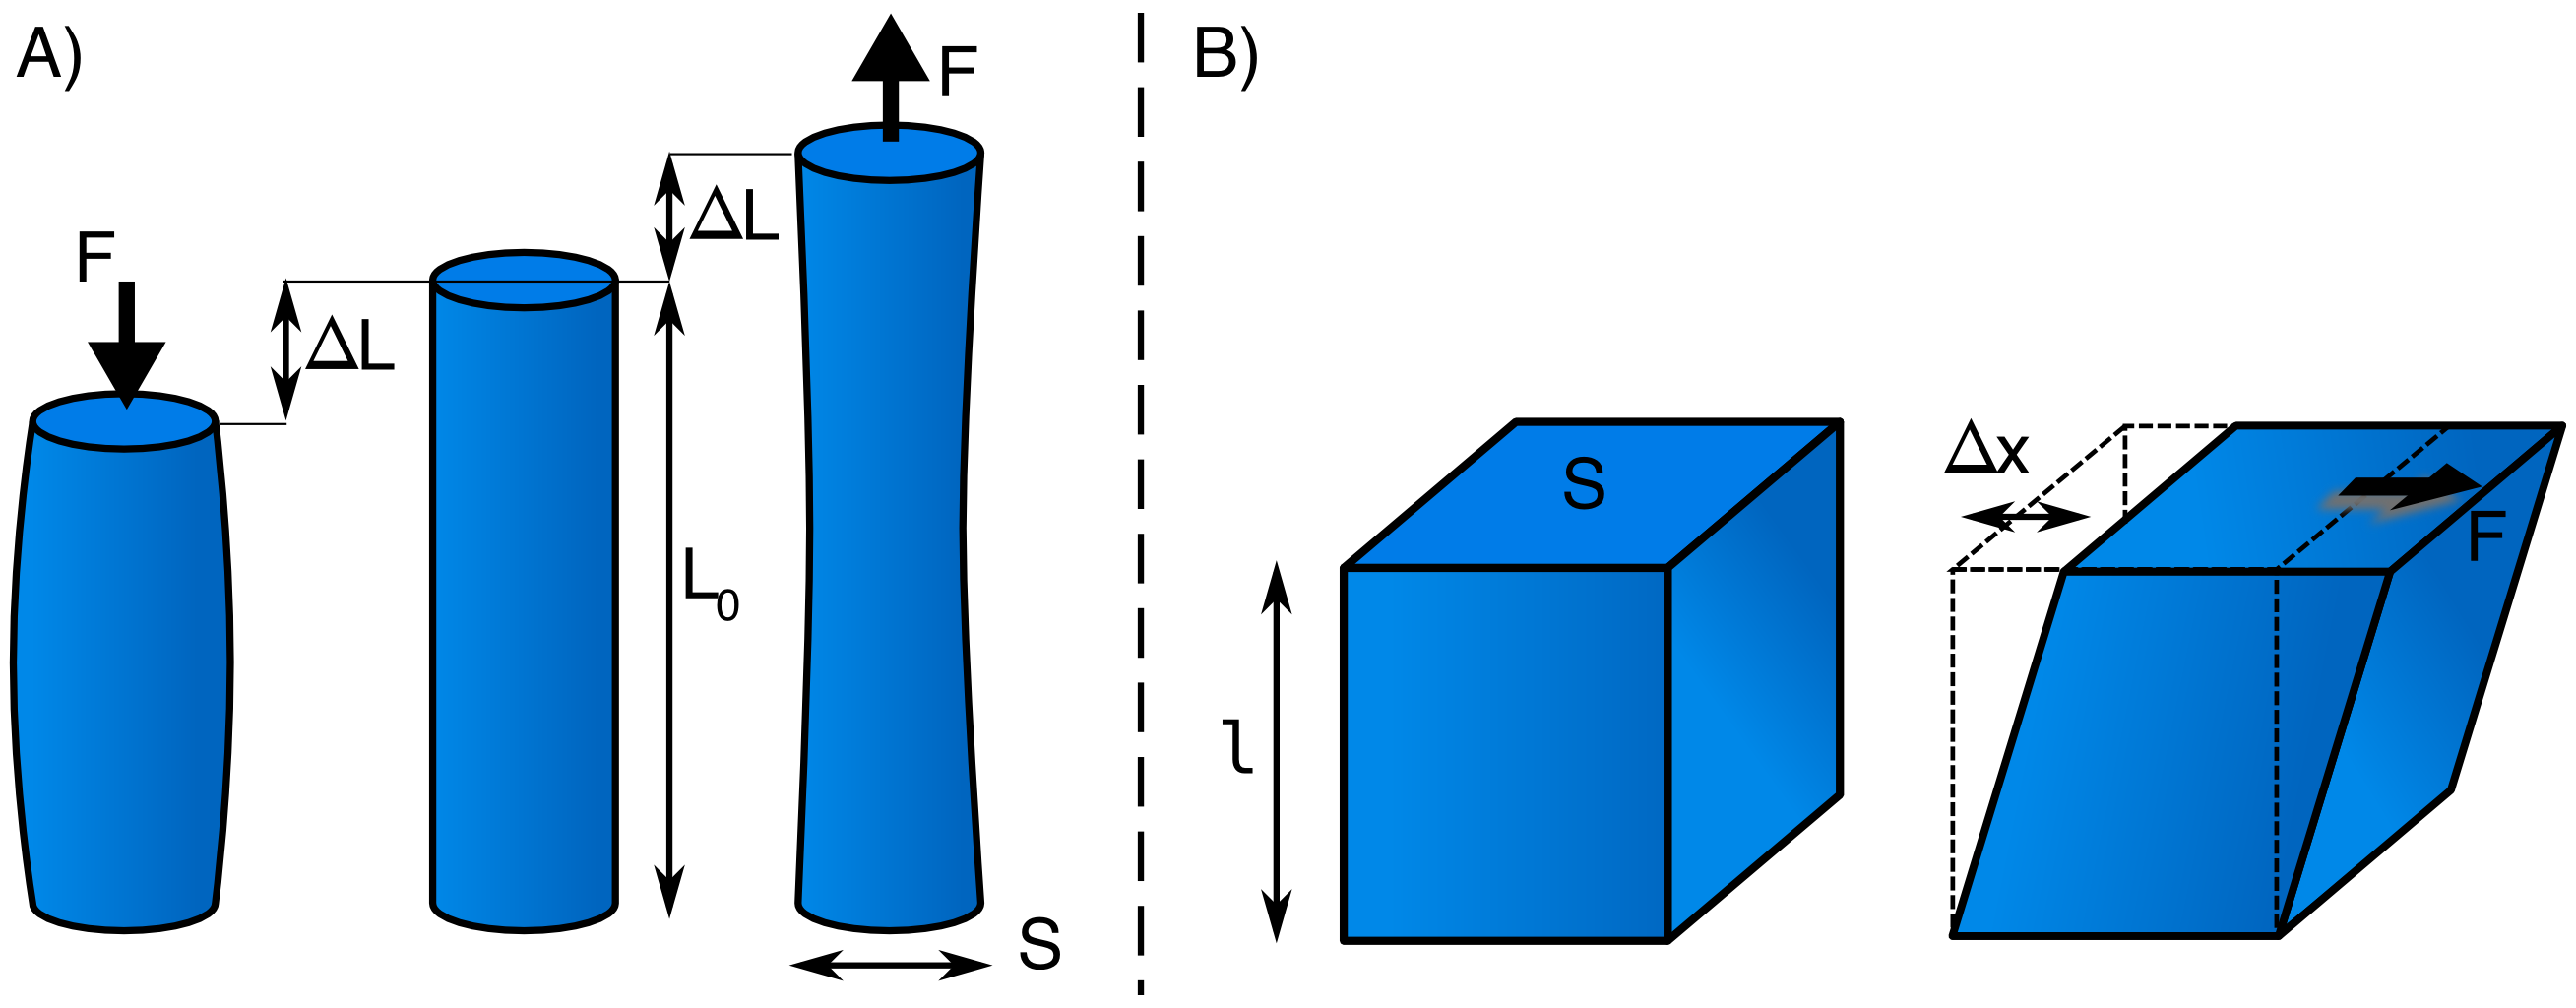
\includegraphics[width=0.800\linewidth]{youngm.png}
\caption{Schematic of the Young Modulus definition. F, force applied to a sample, S
surface of cross section when uncompressed, \(L_0\), length when no load
is applied. For both compression and extension, in the regime of small
deformation, the relative change of length is proportional to the applied
force. Here, the material can be seen to expand/contract in the orthogonal direction
to the direction of the, applied force. In the case of an
incompressible material (\(\nu = 0.5\)) this can be seen as the
conservation of the material volume.}\label{index-latex:fym}\end{figure}

The shear modulus is defined for a deformation, parallel to the surface on which it is applied :
\phantomsection\label{index-latex:equation-eqa9}\begin{gather}
\begin{split}G &= \frac{\tau_{xy}}{\gamma_{xy}} \\
  & = \frac{   F/S }{   \Delta x / l        }\end{split}\label{index-latex-eqa9}
\end{gather}
In which \(\tau_{xy}\) is the shear stress, \(\gamma_{xy}\) is the shear strain, \(F\) is the applied force
on the cross section of the material \(S\). \(l\) is the thickness of the material and \(\Delta x\) is the
transverse displacement (\hyperref[index-latex:fym]{Figure  \ref*{index-latex:fym}} B).

Other characteristic numbers can also be defined, such as the bulk modulus. In the case of isotropic
elastic materials, only two of those parameters are required to completely define
the properties of the material.


\subsection{Poisson's Ratio}
\label{index-latex:poisson-s-ratio}
We have seen that the shear modulus is linked to the Young modulus using
the Poisson's ratio. It is another characteristic of a material
that defines how much a material will compress/expand in the orthogonal directions to its elongation.
The Poisson's ratio is the negative ratio of transverse to axial strain :
\phantomsection\label{index-latex:equation-eqa10}\begin{gather}
\begin{split}\nu = - \frac{
    d \epsilon_{trans}
}{
    d \epsilon_{axial}
}\end{split}\label{index-latex-eqa10}
\end{gather}
In which \(\epsilon_{axial}\) is the relative deformation along one of the
axis of compression/elongation and \(\epsilon_{trans}\) corresponds to the
relative deformation along an axis, orthogonal to the axis of deformation.

Volume conservation during compression or elongation requires
a Poisson's ratio of \emph{0.5}. Such values have been found in bulk measurements of
actin networks at actin concentrations of 21.5 µM in G-actin {\hyperref[index-latex:gardel2003]{{[}Gardel et al. 03{]}}}. Materials with a Poisson's ratio of \emph{0.5} are
said to be incompressible. A Poisson's ratio lower than \emph{0.5} corresponds to materials
expanding less than incompressible materials, and some cells and tissues are known to
have a Poisson's ratio lower than 0.5 {\hyperref[index-latex:mahaffy2004]{{[}Mahaffy et al. 04{]}}}. Another critical value
is 0, where the materials only expand or contract in the direction of the
main stress.

Materials with a Poisson's ratio superior to 0.5 would show a bigger
deformation in the orthogonal direction than incompressible materials, leading
to a global volume increase, if compressed.


\subsection{Viscosity}
\label{index-latex:viscosity}
Like elasticity, viscosity is something tangible we are used to work with in
everyday life. The more viscous a material is, the more difficult it is to move
something in it, at high speed. And indeed, viscosity is the pendant of the elastic
modulus, but considering forces induced by the deformation rate instead of displacement
\phantomsection\label{index-latex:equation-eqa12}\begin{gather}
\begin{split}\frac{F}{S} &= \tau_{xy} \\
            &= \eta \frac{\partial v}{\partial z}\end{split}\label{index-latex-eqa12}
\end{gather}
In which \(\tau_{xy}\) is the shear stress, \(F\) is the force exerted
on the surface \(S\). \(\eta\) is the viscosity, and is expressed in
\(Pa.s\), \(v\) is the deformation rate along the direction \(z\) .

At room temperature, water has a viscosity of around 1 mPa.s, and honey of 10 Pa.s. The consideration of viscosity in problems will
often depend on the timescale and deformation rate. At a short
timescale, tissue often behaves elastic, whereas at a long timescale, the effect
of viscosity will be seen {\hyperref[index-latex:thoumine1997]{{[}Thoumine et al. 97{]}}}. In actin networks, the effect of
viscosity at short time scale can be similar to elasticity {\hyperref[index-latex:gardel2003]{{[}Gardel et al. 03{]}}}.


\subsection{Viscoelasticity}
\label{index-latex:viscoelasticity}
Typically, no material is purely elastic or purely viscous. While glaciers
seem purely solid at the time scale of a few days, observation on a longer time
scale, ranging from months to years, show that ice is not only a
solid, but can also flow. Of course, ice in its solid form is not the only
material which is both solid and viscous. In order to describe such
behaviour, one can use the theory of viscoelastic materials.  A number of models have
been and are still developed to describe viscoelastic behavior. The
Kelvin-Voigt and Maxwell models are two of the simpler ones (\hyperref[index-latex:fig-mkv]{Figure  \ref*{index-latex:fig-mkv}}). A thought
experiment, conducted to understand each of these models, consists of putting a spring and a dash pot
in parallel or series. Such model systems exhibit viscoelastic behavior.
\begin{figure}[htbp]
\centering
\capstart

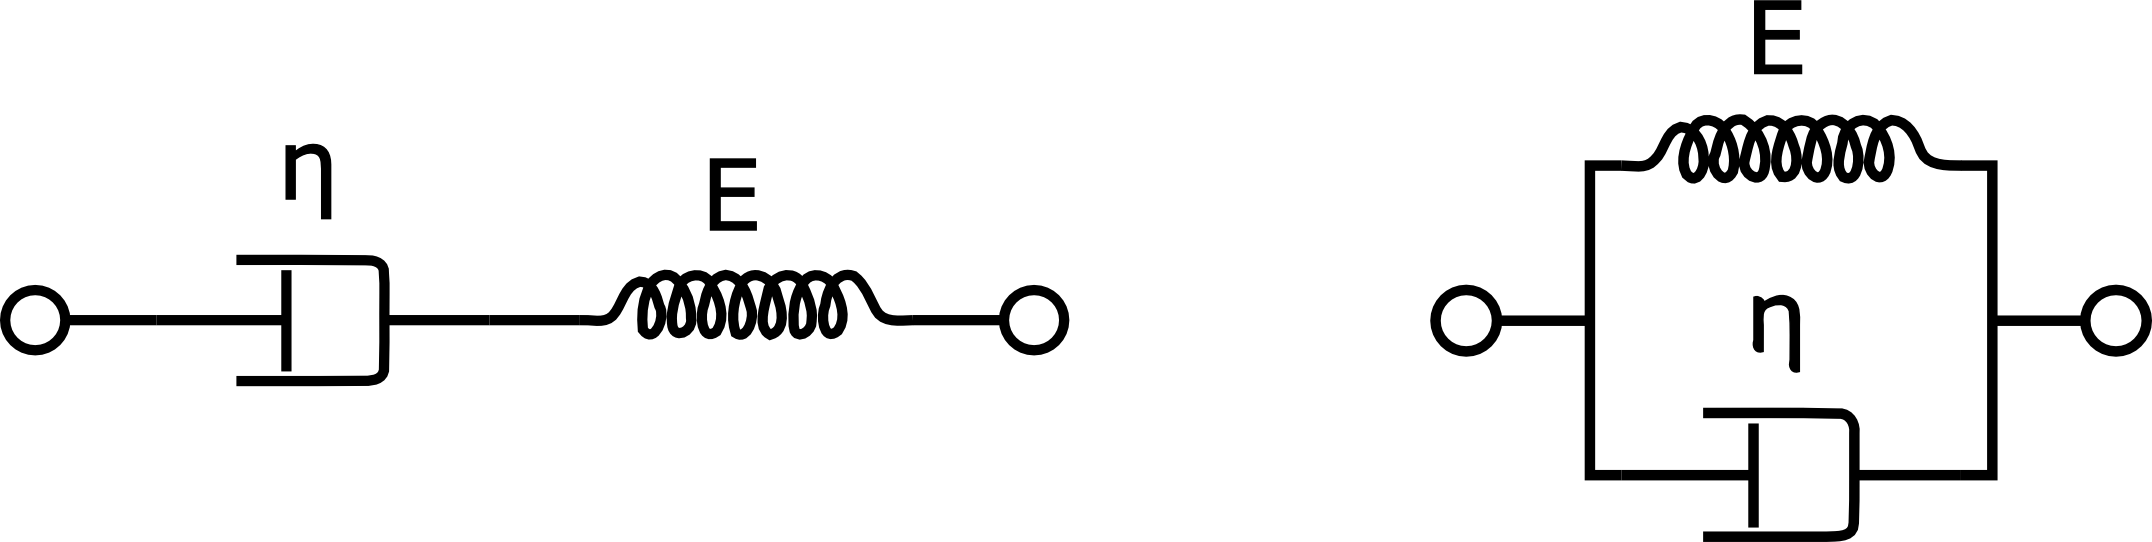
\includegraphics[width=0.700\linewidth]{MKV.png}
\caption{Maxwell model schematic on the left and Kelvin-Voigt model on the right.
Both are simple approaches to express the properties of a viscoelastic
solid. The response to a creep compliance will differ in both cases. The Maxwell
model will mostly behave like a fluid with viscosity \(\eta\) after a
long time, whereas the Kelvin-Voigt model will mostly reflect the elastic
components at constant exerted stress. (Schematic in Public Domain, adapted
from Wikimedia).}\label{index-latex:fig-mkv}\end{figure}

The idea for more complex models is similar: any material can be considered as an
(infinite) combination of springs (for elasticity), and dash-pots, (for viscosity).

The theory of viscoelastic materials explains the mechanical properties of a system by
using a single parameter: the viscoelasticity of a material. This can
be done by describing \(E\) as a relaxation modulus depending on time.  In
the case of a linear system, we can express the strain on the material at a given
time, as a function of its history :
\phantomsection\label{index-latex:equation-strain}\begin{gather}
\begin{split}\sigma (t)  = \int_{-\infty}^t E(t-\tau) \frac{du}{d\tau} d\tau\end{split}\label{index-latex-strain}
\end{gather}
In which \(\sigma(t)\) is the time dependent stress, and \(u(t)\) is
the known strain.

Through the use of rheology, it is common to measure the properties of a material using a
sinusoidal strain of known amplitude \(u_0\) and frequency \(f =
\omega/ 2.\pi\) : \(u(t) = u_0.cos(\omega t)\), which also implies a
sinusoidal strain rate. Using the complex notation \(\dot u = u_0 i\omega
e^{i\omega t}\) in equation \eqref{index-latex-strain}, and operating the change of variable \(t-\tau \to t'\)  leads to :
\phantomsection\label{index-latex:equation-eqa13}\begin{gather}
\begin{split}\sigma(t) = u_0\int_0^\infty E(t') i\omega e^{i\omega(t-t')}dt'\end{split}\label{index-latex-eqa13}
\end{gather}
By factoring out the time dependent part, the rest can be rewritten as two integrals with respectively a real and an imaginary prefactor:
\phantomsection\label{index-latex:equation-eqt}\begin{gather}
\begin{split}\sigma(t) = u_0e^{i\omega t}\times\left(
          \omega \int_0^\infty E(t')  sin(\omega t) dt'
          +
        i \omega \int_0^\infty E(t') cos(\omega t) dt'
\right)\end{split}\label{index-latex-eqt}
\end{gather}
The two integrals in brackets only depend on the pulsation \(\omega\) and the properties of the considered material.
They are both in factors of the complex strain \(u(t) = u_0 e^{i\omega t}\).
We thus define the storage modulus of the material as the real part of (\eqref{index-latex-eqt} in bracket) \(E'\) :
\phantomsection\label{index-latex:equation-eqa14}\begin{gather}
\begin{split}E'(\omega) =  \omega \int_0^\infty E(t')  sin(\omega t) dt'\end{split}\label{index-latex-eqa14}
\end{gather}
And the loss modulus as the imaginary part of (\eqref{index-latex-eqt} in bracket)
\phantomsection\label{index-latex:equation-eqa15}\begin{gather}
\begin{split}E"(\omega) =  \omega \int_0^\infty E(t')  cos(\omega t) dt'\end{split}\label{index-latex-eqa15}
\end{gather}
And define the complex frequency dependent Young's modulus as :
\phantomsection\label{index-latex:equation-eqa16}\begin{gather}
\begin{split}E^*(\omega) = E'(\omega) + i.E"(\omega)\end{split}\label{index-latex-eqa16}
\end{gather}
Thus we can write \eqref{index-latex-eqt} as :
\phantomsection\label{index-latex:equation-eqa17}\begin{gather}
\begin{split}\sigma(\omega) = E^*(\omega).u(\omega)\end{split}\label{index-latex-eqa17}
\end{gather}
In this representation of \(E^*(\omega)\), the real part will correspond to
the elastic response of the material (in-phase response
under oscillatory strain) and the imaginary part corresponds to the viscous response
of the system (out of phase under sinusoidal strain). The complete knowledge of
\(E^*(\omega)\) at all frequencies completely characterizes the material.

.

Models for actin networks have been extensively studied as viscoelastic material
both theoretically {\hyperref[index-latex:morse1998a]{{[}Morse 98a{]}}}, {\hyperref[index-latex:kruse2005]{{[}Kruse et al. 05{]}}} , and  experimentally
{\hyperref[index-latex:mizuno2007]{{[}Mizuno et al. 07{]}}}. Actin networks have also been shown to exhibit linear characteristic behavior,
but at certain concentration ranges, a non-linear behavior has also been observed {\hyperref[index-latex:yao2011]{{[}Yao et al. 11{]}}}, {\hyperref[index-latex:gardel2003]{{[}Gardel et al. 03{]}}}.

The actin networks we will study hereafter, being in the condition where a linear behavior is expected, we will thus use the viscoelastic theory to interpret the
observed relation stress/strain, in order to determine the mechanical properties
of the formed actin gels.


\section{Optical tweezer}
\label{index-latex:optical-tweezer}\label{index-latex:id77}
Optical tweezers, or optical traps, are a technique that allows to trap objects
near the focal plane of a microscope, at the focal point of a high-power laser.
It is a versatile technique that allows to trap both fabricated objects and
parts of living cells. Optical traps typically allow to apply forces up to a few tenth of
pico Newton.

In order to understand that light can trap an object, it is instructive to keep in mind
that, despite having no mass, photons carry momentum and that, as for any massive
object, changing the trajectory requires a force.  According to Newton's third
law, when applying a force via a photon on an object, the object will in turn
exert the opposite force on the photon, thus changing its trajectory. If a photon changes its trajectory in a material, the material has to apply a
force on it(\hyperref[index-latex:setup]{Figure  \ref*{index-latex:setup}}), meaning that the photon also applies a force on the
material. In particular, the higher the refractive index of a material, the
more light beams are deviated, and hence the more photons apply forces on
material.

More specifically, it can be shown that objects with a higher refractive
index than the surrounding medium, are attracted towards higher light intensities
(\hyperref[index-latex:setup]{Figure  \ref*{index-latex:setup}}).  In particular, laser beams with a Gaussian intensity
profile, will lead to the object being attracted towards their center.

In addition to the lateral trapping, the laser focus leads to
another intensity gradient along the direction of beam propagation, the intensity being at its maximum at the laser waist.

So, a laser coupled into a microscope objective acts as a three dimensional
potential that traps particles, similar to a tweezer. Usually the trapping in
a parallel to the laser direction, is only about half as strong if compared to the trapping in the
lateral direction.
\begin{figure}[htbp]
\centering
\capstart

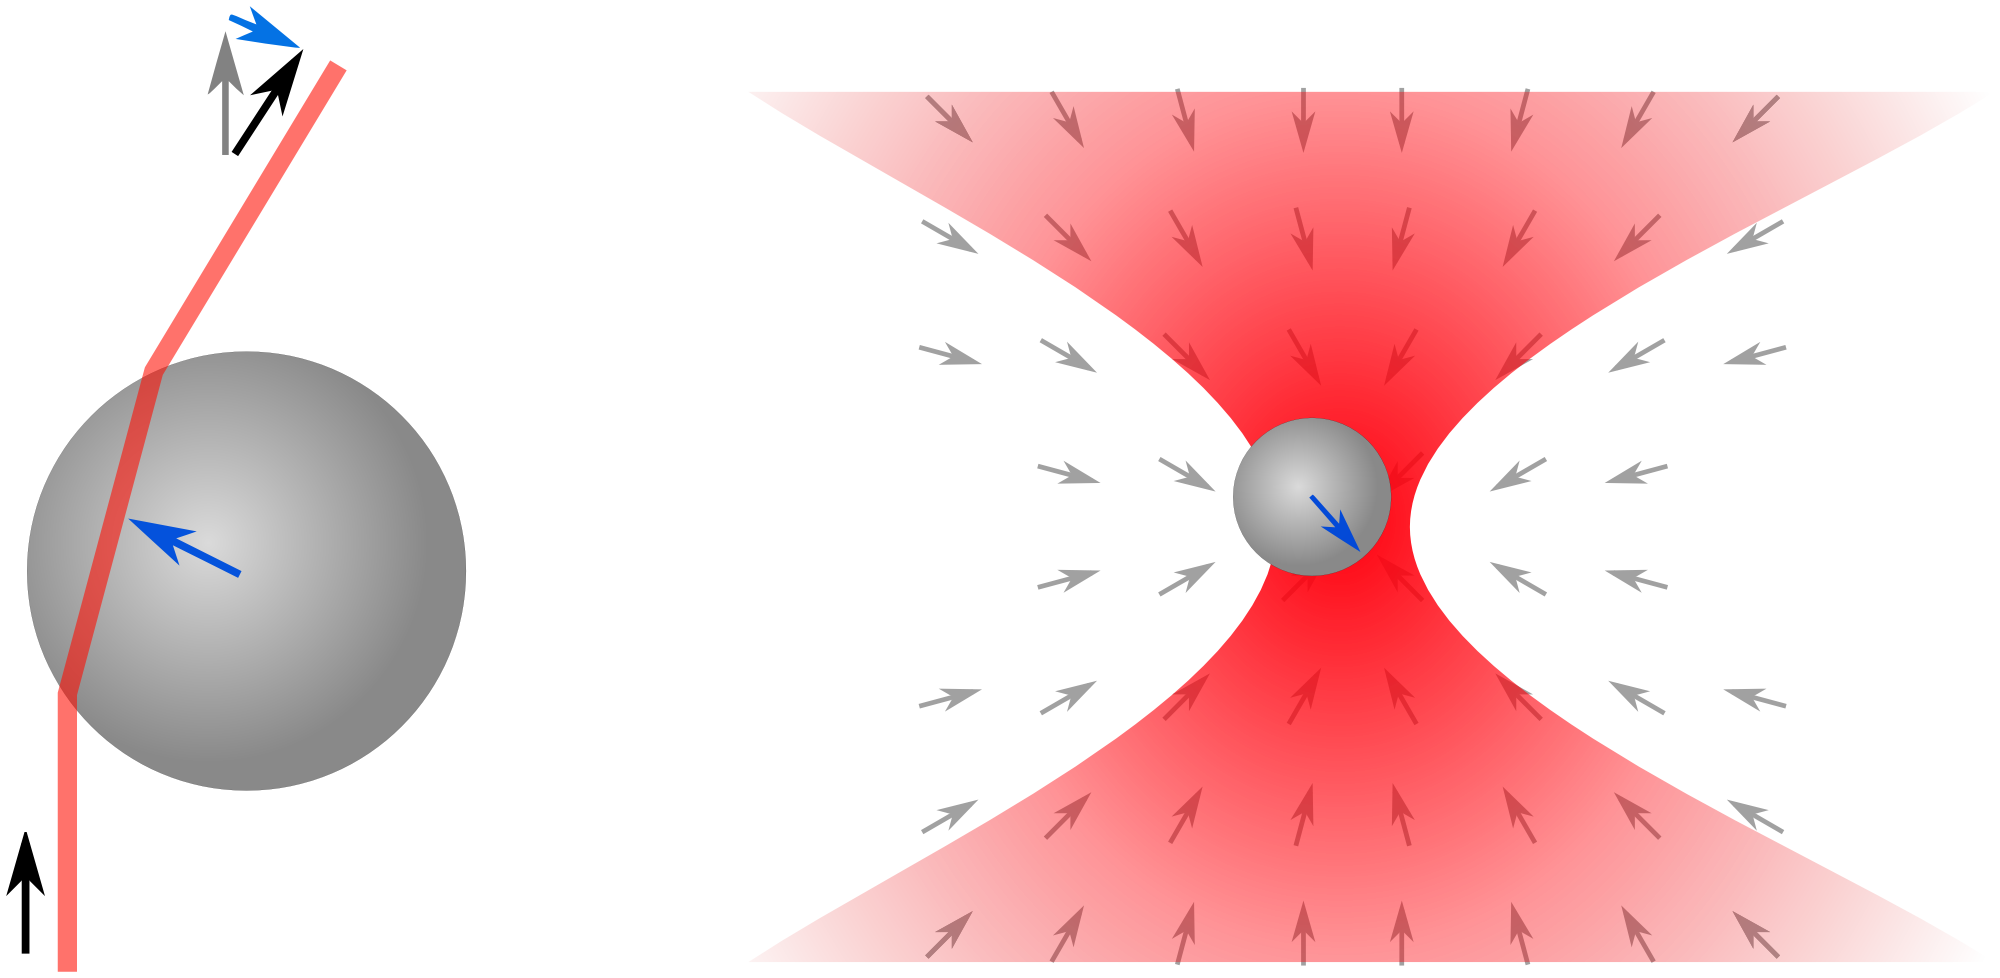
\includegraphics[width=0.700\linewidth]{ot1.png}
\caption{Light deflected by a transparent bead changes the light momentum, so the
light is exerting a force on the bead, which will be attracted towards
the highest intensity.  For a focused laser beam, the bead will be attracted
near the laser focus.}\label{index-latex:setup}\end{figure}

Among the qualities of optical traps, one is that in principle, multiple traps can be
obtained. A simple method to generate two traps is to split the incoming light
into two orthogonally polarized independent beams.  Instead of sharing the
laser power between the different traps by using polarisation, one can use what
is known as multiplexing by time sharing. This is achieved by rapidly switching the laser
between different positions at a much faster speed than the diffusion of the particles. By using this method,
it is possible to virtually achieve multiple traps on the same
sample.

In this work, we use a multiplexed system, where the rapid switching is achieved, by means of Accousto Optic Deflectors
(aka AODs).  An AOD consists of a crystal in which a high frequency
sound-wave propagates perpendicular to the incoming laser beam. This sound-wave generates local changes in the
refractive index of the material, which acts as a diffraction grating. In
the right conditions, a laser passing through the crystal will
be deflected by this grating under the Bragg angle.

In practice, rapidly controlling the frequency and amplitude of the sound-wave
in the crystal, allow direct adjustment of laser deflection and hence the
trap position. Not only does the use of AODs offer the advantage of controlling
the number and position of multiple traps, but also the individual power allocated to each trap, hence their stiffness.
.. \_ots:
\begin{figure}[htbp]
\centering
\capstart

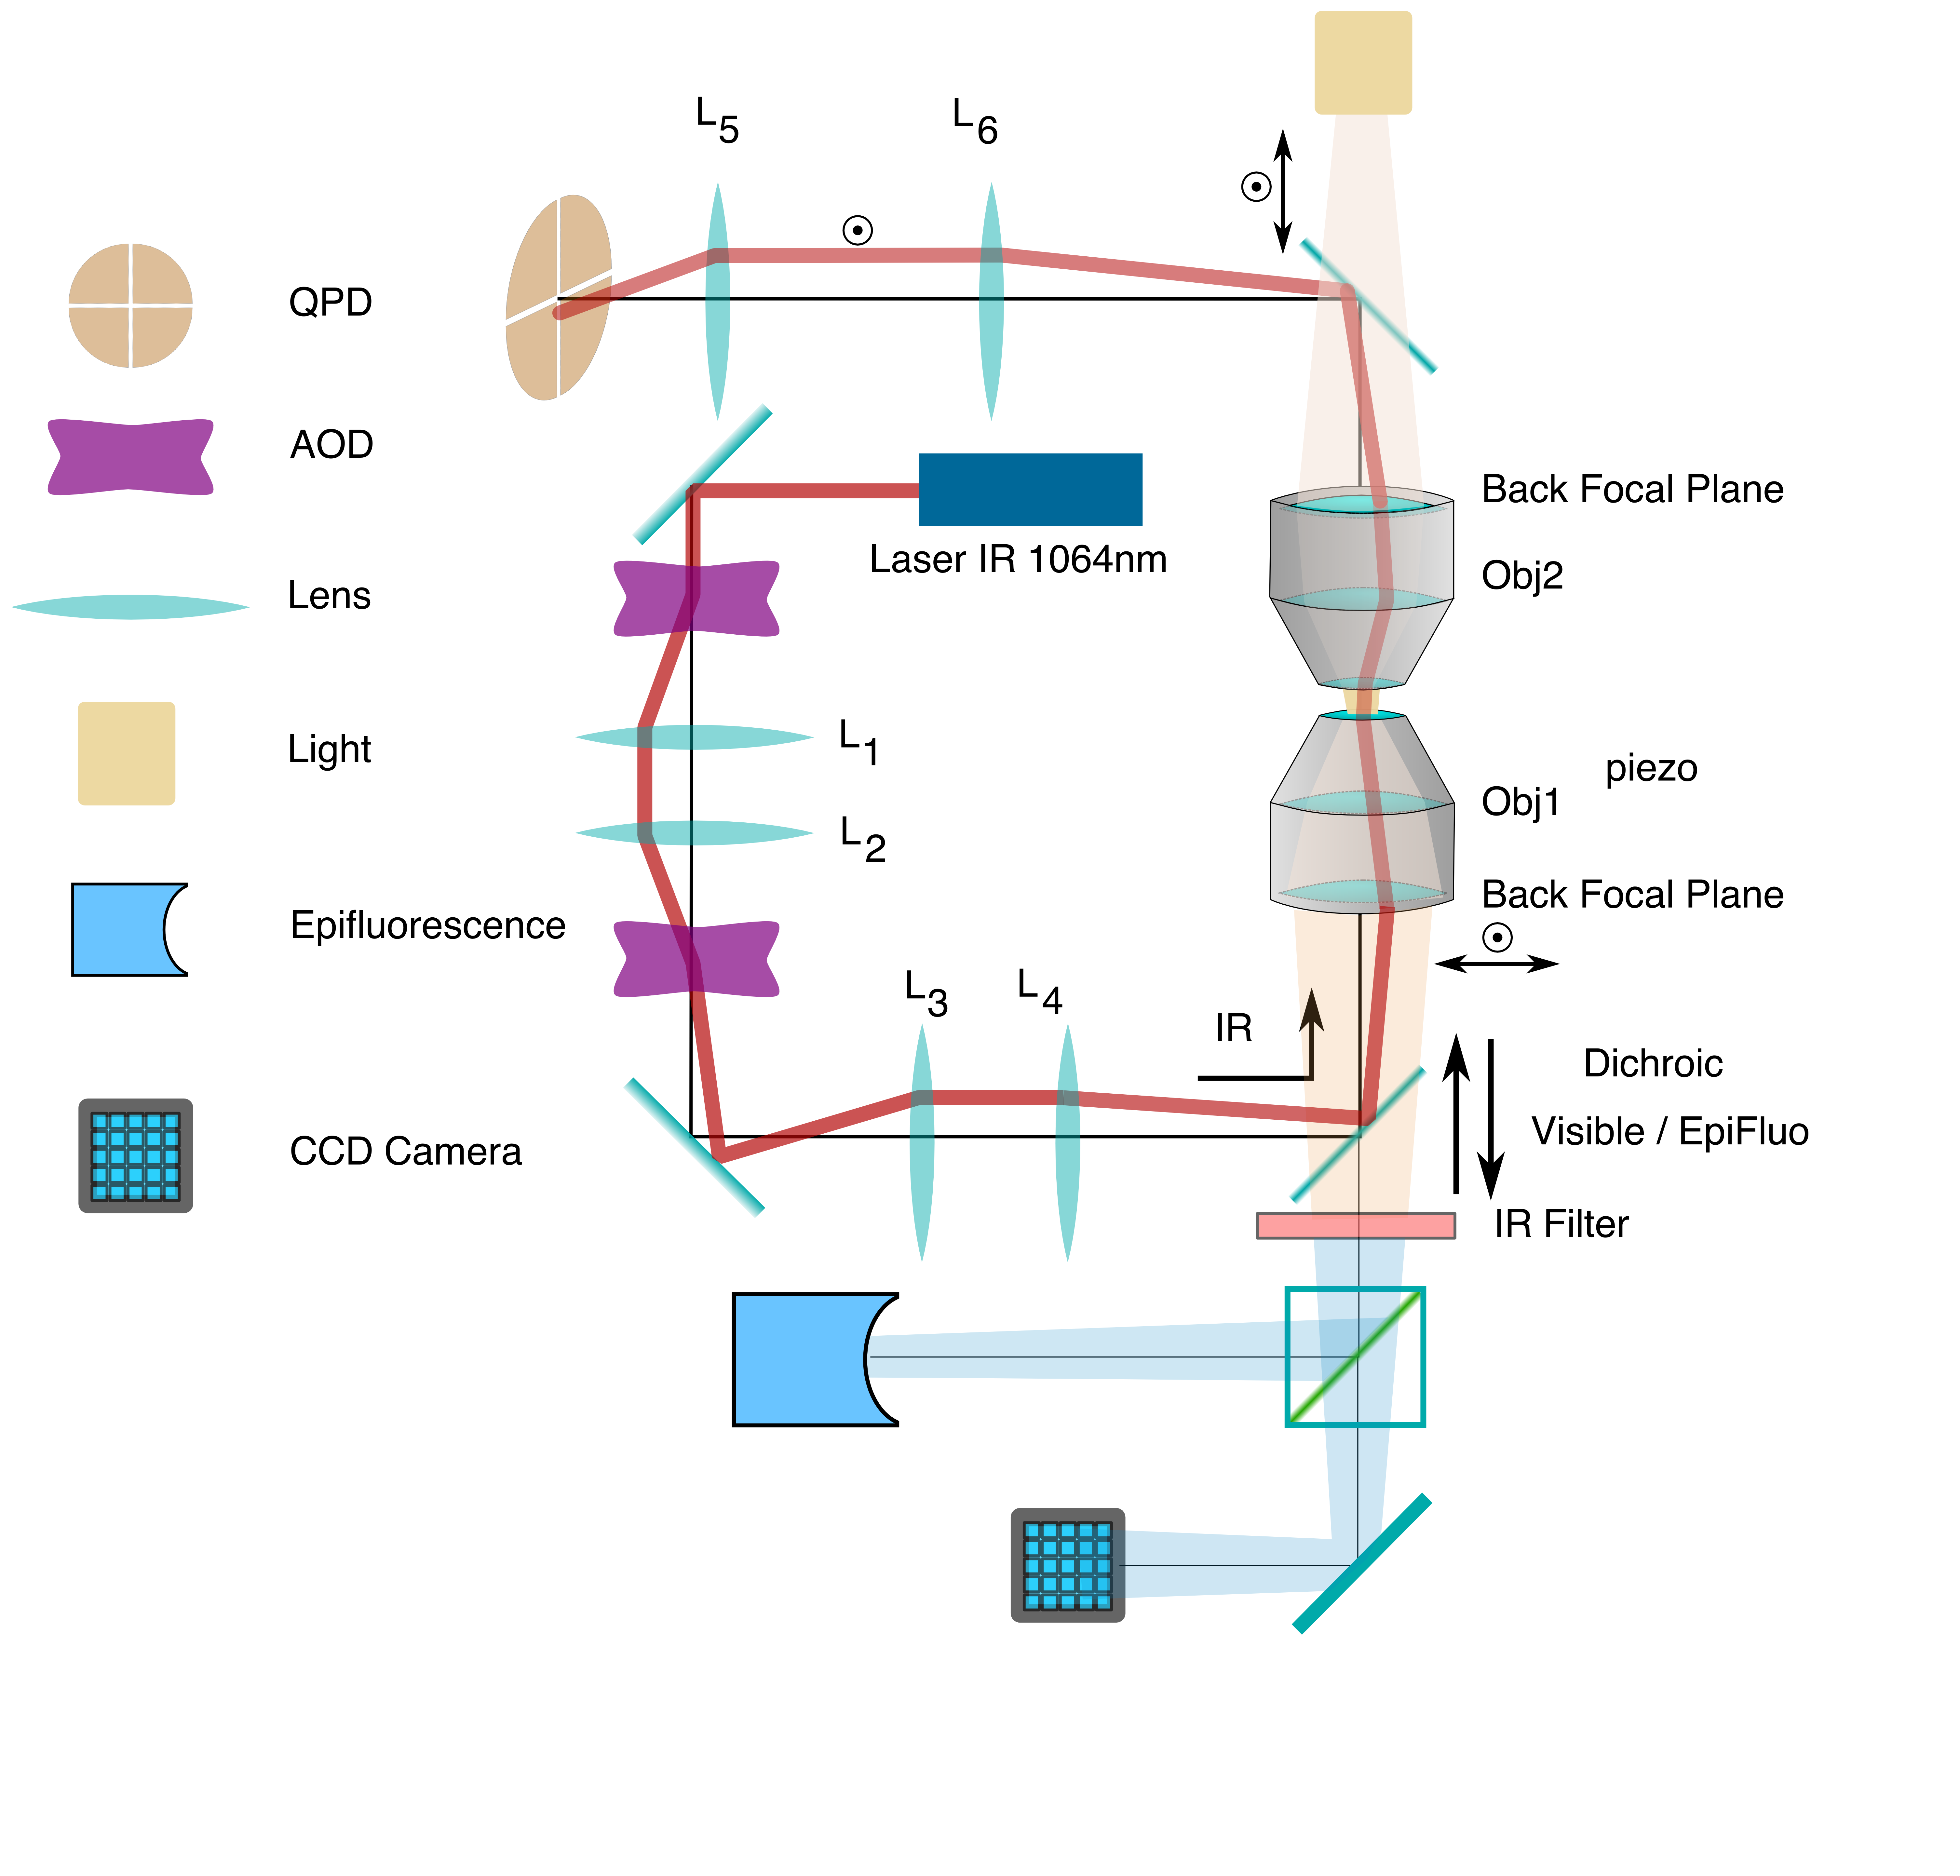
\includegraphics[width=0.900\linewidth]{setup-plus-1.png}
\caption{A schematic of  setup used. The following elements can be distinguished. An
1064nm laser is used for trapping. It first passes through two AODs that
move the position of the trap in the X  and Y direction.  The first couple
of lenses (L1,L2) between AODs assures that AODs are in conjugated planes.
The second pair of lenses (L3,L4) image the AODs plane in the back-focal plane
of the first objective.
Thus, a change of angle of the light beam induced by the AOD,
results in a  change of the trap position.  The trapping light
is collected by a second objective, and illuminates a quadrant photodiode
(QPD) conjugated to the back focal plane of the collecting objective. By
construction, QPD and AODs should be conjugated, so the deviation of the light
beam induced by one of the AODs is not supposed to induce any change of
the laser spot position on the QPD. Additional dichroic mirrors allow to
use bright field and epifluorescence simultaneously with the optical
tweezer.}\end{figure}

A schematic of the optical setup used to trap beads in the focal
plane on the microscope, can be found in \hyperref[index-latex:ots]{figure  \ref*{index-latex:ots}}. The scheme also
contains the detection part of the setup used to measure the force
exerted on each bead, technique which is explained in the following part.


\subsection{Determination of trapping forces and bead displacement}
\label{index-latex:determination-of-trapping-forces-and-bead-displacement}
In addition to allowing the objects to be held in place, the use of a QDP
(Quadrant Photo Diode, a precise position detector) with optical traps, has the
advantage to acquire the high frequency quantitative measurements of the
displacement and force exerted on an object.  Indeed, when the trapped particle
is not in the trap center, the laser applies a force on the object.
Reciprocally, the object applies the opposite force on the light beam, thus
deflecting it.  With a proper use of optics and lenses correctly placed on the
Fourier plane of the sample, it is hence possible to translate this orientation
change of the light  beam into a displacement of a light spot, onto a photo
detector with high sensitivity to applied forces.

Through a careful calibration of the trap, which gives the force/displacement
relationship, {\hyperref[index-latex:jahnel2011]{{[}Jahnel et al. 11{]}}}, {\hyperref[index-latex:vermeulen2006]{{[}Vermeulen et al. 06{]}}}, one can then also
recover the sample displacement inside the optical trap.

Using an optical tweezer, not only aiming at holding a particle in position, but also at getting a
quantitative measurement of its displacement and the exerted force, requires to
calibrated each probe particle. Polystyrene beads are common artificial probes,
used to achieve such a goal.

The use of polystyrene beads has multiple advantages. First, one
can obtain mono-dispersed beads, leading to reproducible and predictable trap
stiffness. Secondly, theory can predict the shape of
the potential felt by such a bead in a Gaussian beam {\hyperref[index-latex:nieminen2007]{{[}Nieminen et al. 07{]}}}.

The third advantage is that beads can be fictionalized, allowing specific
interaction to be controlled, both \emph{in vitro} and \emph{in vivo}. Of course, the
calibration is essential for the correct measurement of the different systems mechanical property
, and the choice of the bead diameter has an impact both on
the biological side and in the measurement physics.
\phantomsection\label{index-latex:part2}

\chapter{Materials and Methods}
\label{index-latex::doc}\label{index-latex:part2}\label{index-latex:materials-and-methods}\label{index-latex:m-et-m}

\section{Buffers}
\label{index-latex:buffers}

\subsection{G-Buffer}
\label{index-latex:g-buffer}
G-Buffer is used to conserve actin in the monomeric form. Actin is diluted in
G-Buffer and kept on ice for at least 12 hours before further use. G-buffer is
aliquoted and stored at -20°C. For weekly use it is thawed and conserved on ice for up to a week. G-buffer is never
refrozen. pH is adjusted to 7.4.

Composition of G-Buffer:
\begin{itemize}
\item {} 
0.2 mM \(CaCl_2\)

\item {} 
0.5 mM DTT (Dithiothreitol, or (2S,3S)-1,4-bis(sulfanyl)butane-2,3-diol)

\item {} 
2.0 mM Tris (tris(hydroxymethyl)aminomethane or 2-Amino-2-hydroxymethyl-propan)

\item {} 
0.2 µM ATP (Adenosine triphosphate)

\end{itemize}


\subsection{Polymerisation Buffer}
\label{index-latex:polymerisation-buffer}
Polymerisation buffer or X-Buffer is used for the polymerisation of actin gels on
beads  as well as bead dilution and buffer cleaning.  It is aliquoted and conserved at
-20°C. During experiments, it is stored on ice for up to a week. X-Buffer is never
refrozen.

Composition of X-Buffer :
\begin{itemize}
\item {} 
10 mM Hepes (2-{[}4-(2-hydroxyethyl)piperazin-1-yl{]}ethanesulfonic acid)

\item {} 
0.1 M \(KCl\)

\item {} 
1 mM \(MgCl_2\)

\item {} 
1 mM ATP (Adenosine triphosphate)

\item {} 
0.1 mM \(CaCl_2\)

\end{itemize}


\subsection{X-Buffer with BSA}
\label{index-latex:x-buffer-with-bsa}
Same as X-Buffer, with the addition of 1\% BSA (10 mg/ml). BSA is used to prevent
non specific adsorption. X-BSA buffer is used  in place of  X-Buffer for
probe-beads conservation.


\subsection{ATP-Mix Buffer}
\label{index-latex:atp-mix-buffer}\label{index-latex:id1}
ATP-Mix buffer or simply \emph{Mix} contains the required  ATP for actin
polymerisation. It is aliquoted and stored at -20°C. Kept on ice for weekly use. pH is adjusted to 7.4.
\begin{itemize}
\item {} 
12.0 mM ATP,

\item {} 
20,0 mM DDT

\item {} 
0.88 mM Dabco

\item {} 
24.0 mM \(MgCl_2\)

\end{itemize}


\section{Protein preparation}
\label{index-latex:protein-preparation}

\subsection{pWA (also called pVCA)}
\label{index-latex:pwa-also-called-pvca}
pWA is used as a nucleation promoting factor. It is expressed from Human pVCA
(verprolin homology central and acidic domain) into Rosetta
2(DE3) pLysS (Novagen) Cell.  Purified pWA is aliquoted and conserved at -80°C, never
refrozen, and conserved on ice for daily use.


\subsection{Actin}
\label{index-latex:actin}
Actin and biotinylated actin are purchased from Cytoskeleton (Denver, CO, USA), and stored at -80°C.
Fluorescent Alexa-488 actin is obtained from Molecular Probes, stored at -80°C, and prepared according to manufacturer recommendation.

Actin is stored in 5µL aliquots at a concentration of \textasciitilde{}238 µM, and
fluorescent actin in 3µL aliquots at a concentration of \textasciitilde{}106 µM.

G-actin with 20\% fluorescently labeled actin monomers is prepared the day before
the experiment, by mixing 1 aliquot of actin with 1 aliquot of fluorescently
labeled actin, and by diluting the mix with G-Buffer until the desired concentration is reached.


\subsection{Profilin}
\label{index-latex:profilin}
Human profilin is expressed by competent cells and purified in our laboratory as
described in {\hyperref[index-latex:carvalho2013a]{{[}Carvalho et al. 13a{]}}}.  Profilin is conserved at 4°C for a few months and
kept on ice for daily use.


\subsection{Arp2/3}
\label{index-latex:arp2-3}
Bovine Arp2/3, complex, is purchased from Cytoskeleton, prepared as recommended by the manufacturer, aliquoted at 1µM
and conserved at -80°C.  Aliquots are never refrozen and stored on ice for
weekly use.


\subsection{Capping protein}
\label{index-latex:capping-protein}
Mouse capping protein (CP; a1/b2) is purified as previously described in {\hyperref[index-latex:soeno1998]{{[}Soeno et al. 98{]}}}. CP was a gift from Laurent Blanchoin.


\subsection{Myosin II}
\label{index-latex:myosin-ii}
Myosin II is purified from rabbit skeletal muscle and fluorescent myosin II is
prepared as previously described in {\hyperref[index-latex:soaresesilva2011]{{[}SoareseSilva et al. 11{]}}}. The Myosin II functionality
is confirmed by motility assays. Gliding speed shows an average of 4.5
+ 1.5 µm/s (N = 27).

The working buffer for Myosin contains
\begin{itemize}
\item {} 
25 mM imidazole

\item {} 
50 mM \(KCl\)

\item {} 
70 mM sucrose

\item {} 
1mM Tris

\item {} 
2 mM \(MgCl_2\)

\item {} 
1 mM ATP

\item {} 
0.1 mM DTT

\item {} 
0.02 mg/ml \(\beta\)-casein,

\end{itemize}

Then,  pH is adjusted to 7.4.
In the working buffer, myosin II
forms monofilaments about 0.7 µm long, which roughly correspond to about 100
motors.


\section{Lipids, reagent and proteins}
\label{index-latex:lipids-reagent-and-proteins}
Chemicals are purchased from Sigma Aldricht (St-Louis, Mo, USA, unless stated otherwise.
EPC (l-\(\alpha\)-phosphatidylcholine) and \emph{1,2-distearoyl-sn-glycero-3-phosphoethanolamine-N-{[}biotinyl polyethylene glycol 2000{]}}
(biotinylated lipids), \emph{1,2-dioleoyl-sn-glycero-3-phosphocholine} are purchased from Avanti Polar Lipids (Alabaster, USA).
Monomeric actin containing 10\% or 20\% of labeled Alexa-488
actin and 0.25 \% of biotinylated actin is diluted in G-Buffer


\section{Doublet preparation}
\label{index-latex:doublet-preparation}\label{index-latex:electroformation}
Cell-sized liposomes are formed by electro formation {\hyperref[index-latex:angelova1986]{{[}Angelova et al. 86{]}}}.
A 20 µL mix of EPC lipids and PEG-biotin lipids (present at 0.1 \%, mol ),
at a 2.5 mg/ml in chloroform/methanol 5:3 concentration, is deposited on glass
plates coated with  ITO. Glass is then dried with  nitrogen and placed
under vacuum for 2 hours.

A chamber is formed, using the ITO plates with their conductive sides facing
inside, then filled with sucrose buffer (200mM sucrose, 2mM Tris adjusted  to a pH of
7.4). The. Chamber  is finally sealed with hematocrit paste (Vitrex Medical, Denmark).

An alternate current voltage of 1V at 10 Hz is applied between the ITO-coated
surfaces for 75 minutes, to form liposomes.

The same preparation is done a second time and, by adding 0.9µm sulphorhodamin to
the sucrose buffer,  the liposomes inside buffer are marked fluorescently.

The two solutions are mixed in order to have the inside buffer of half the
liposomes marked in red, and being to be able to distinguish the interface in some of
the formed doublets.

The formed liposomes are incubated 15 minutes with 160 nM streptavidin in order to
get them coated with it. Streptavidin-coated liposomes tend to
aggregate.  The solution containing doublets is then diluted 30 times. Waiting
15 minutes increases the ratio doublets/single liposomes, by still avoiding
the aggregates of more liposomes.

A bulk solution of 40 µM actin monomers — 10\% fluorescent and 0.25\% biotinylated — is
diluted 40 times in a working buffer (25 mM imidazole, 50 mM KCl, 70 mM sucrose,
1mM Tris, 2 mM \(MgCl_2\), 1 mM ATP, 0.1 mM DTT, 0.02 mg/ml \(\beta\)-casein, adjusted at to a
pH of 7.4) and polymerized for one hour. The adjunction of 1 µm of phalloidin
after 1 hour prevents further depolymerisation.

Actin filaments are
diluted to 0.1 µM (10x), mixed with streptavidin-coated doublets of
liposomes, and incubated for 15 min. The mix is diluted 5 times to reduce the fluorescent background due to actin monomers in solution.


\section{Bead Preparation}
\label{index-latex:id6}\label{index-latex:bead-preparation}
Carboxylated polystyrene beads (Polysciences, Philadelphia, PA) of 4.34 \(\pm\) 0.239
\(\mu\)m (Standard deviation) diameter were used as actin-beads and probe-beads.

Beads are stored at 4°C.

Before being coated by BSA (probe-bead) or pWA (actin-bead), the bead solution is
cleaned by centrifugation at 5000 rpm, 2min. After removing the supernatant, the pellet
is resuspended in X-Buffer. This procedure is repeated twice.


\subsection{Actin-Bead Preparation}
\label{index-latex:actin-bead-preparation}
Cleaned polystyrene beads are incubated for 20 min at 20°C under agitation with
2 \(\mu\)M pVCA. Centrifuged at 5000rpm 2min, the supernatant is removed and the pellet
diluted 4 times in X-buffer. The beads are stored on ice for one day.


\subsection{Probe Bead Preparation}
\label{index-latex:probe-bead-preparation}
Cleaned polystyrene beads are incubated under agitation with 10 mg/ml BSA at
room temperature for 30 minutes. Passivated beads are then centrifuged,
separated from supernatant, the pellet is resuspended in X-BSA buffer and
stored at 4°C for weekly use.


\section{Force indentation experiments}
\label{index-latex:id7}\label{index-latex:force-indentation-experiments}

\subsection{Preparation of sample}
\label{index-latex:preparation-of-sample}
An equal amount of both actin and probe beads are placed in the polymerization
mix consisting of :
\begin{itemize}
\item {} 
2µL BSA at 10\%

\item {} 
3µL of ATP-Mix Buffer

\item {} 
1.5 µL Profilin (114µM)

\item {} 
1 µL beads (50\% actin-bead 50\% probe bead)

\item {} 
0.5 µL Arp2/3 (22,3 µM)

\item {} 
between 0 and 2 µL CP (0.5 µM)

\item {} 
Completed to 15 µL using X-Buffer.

\end{itemize}

5 µL of G-Actin (20\% fluorescent) is then added to the previous mix. This
moment marks the time \emph{t=0} for the experiment and recording. The experimental chamber is
made of 2 coverslips, separated by VaLaP, which is a mix of vaseline (33\%)
Lanoline (33\%) and Parafine(33\%) in equal mass proportion. The chamber is prepared by gently depositing 20 µL of
the final beads mix at the lower coverslip center and 4 drops of VaLaP
where the corner of the upper (18x18mm) coverslip
will rest. The VaLaP, acting as a spacer, prevents the sample from being squashed.  The
upper coverslip is then placed on top of the sample and the chamber is sealed
with VaLaP.


\subsection{QPD positioning and calibration of microscope}
\label{index-latex:laser-calibration}\label{index-latex:qpd-positioning-and-calibration-of-microscope}
The prepared sample is placed on the microscope and a drop of water is
deposited on top of the upper coverslip to assure  the immersion of the light
collecting objective. The collecting objective and the quadrant photodiode are
placed on top of the sample ({\hyperref[index-latex:optical-tweezer]{\emph{Optical tweezer}}} (\autopageref*{index-latex:optical-tweezer})).

The trapping laser is then aligned with the photodiode, checking in the meantime that no
object is trapped during the process. The conjugation of the objective back focal plane
with the AODs and the QPD, is optimized by adjusting the
distance of both objectives with respect to the sample.

A trapping laser is positioned near the center of the microscope field of view,
using the custom written LabView program (\hyperref[index-latex:fig-frontend]{Fig  \ref*{index-latex:fig-frontend}}). The QPD is adjusted in X and Y direction to
\(\Delta X  = \Delta Y = 0V\). This has to be  done while no object is trapped in
the  laser focus.


\subsection{Initial bead trapping}
\label{index-latex:initial-bead-trapping}
Two maximum strength traps (\textasciitilde{}50mW/trap) are created near the center of the
microscope field of view, separated by 15 to 20 µm. The sample plane is then moved in
the Z-direction, by displacing the 3D piezo controlled sample stage, to position the traps
near the chamber middle plane. A temporary removal of the infrared filter
from the microscope allows to see the trapping lasers reflection on both the
upper and lower coverslips and to determine the localisation of the observation chamber middle plane
.
\begin{figure}[htbp]
\centering
\capstart

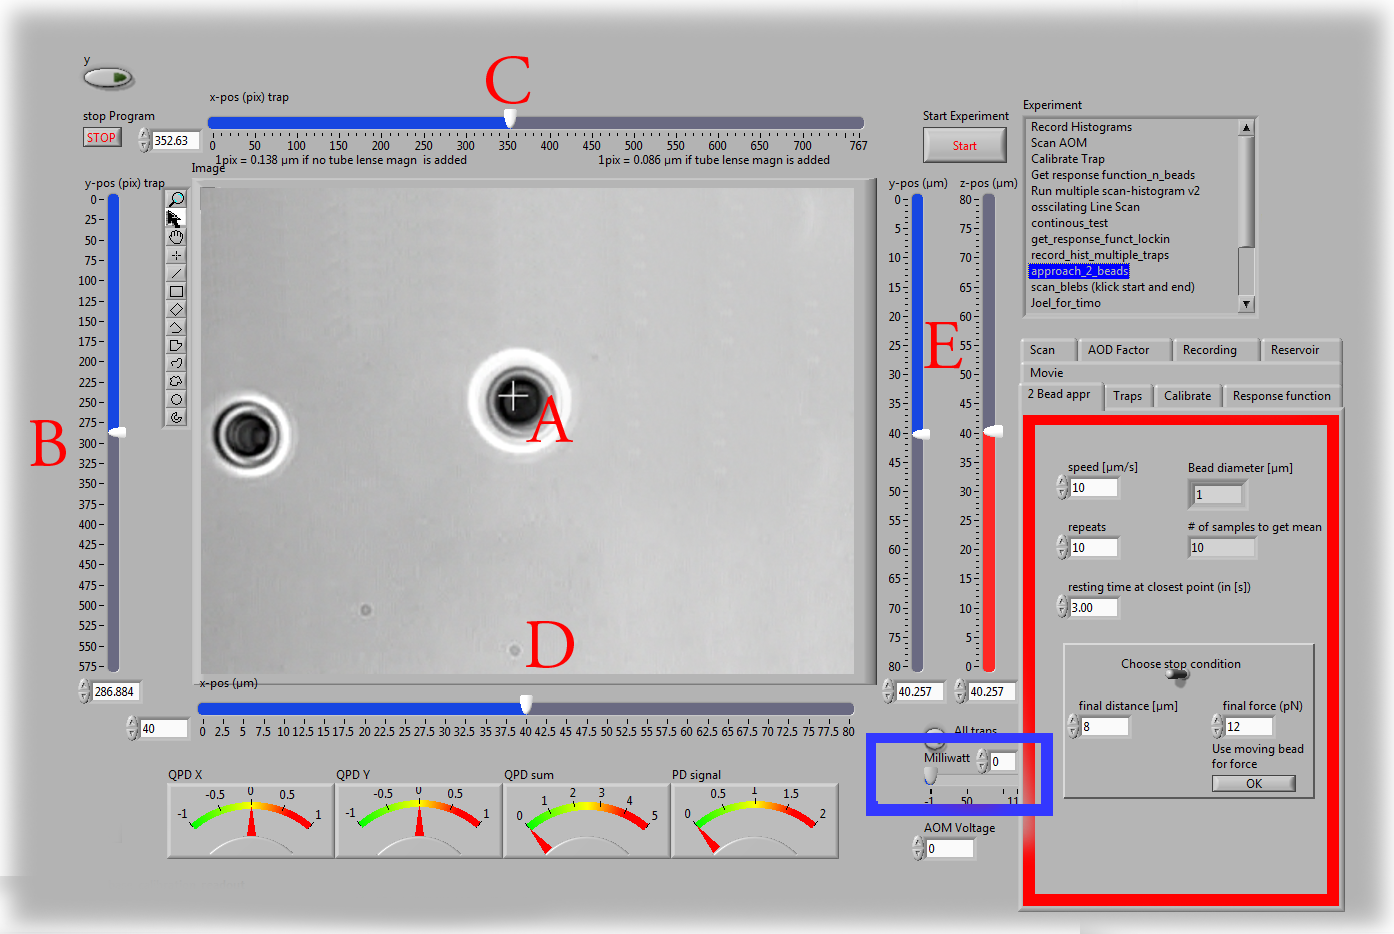
\includegraphics[width=0.900\linewidth]{frontend.png}
\caption{Software interface responsible for controlling the optical tweezer.  Sample
image showing 2 polystyrene beads and a single trap (A, white cross) holding one bead.
Cursors (B,C) are available to displace the optical trap(s).  Cursors can
control the position of the stage: X (D), Y (E, blue) and Z (E,red).
The blue rectangle highlights the slider that allows the control of the traps power.  The red
rectangle highlights the area where the different parameters of the experiment
can be set (approach speed and resting time at closest point). 3 indicators at
the bottom of the screen indicate the voltage on the QPD.}\label{index-latex:fig-frontend}\end{figure}

The operator then captures one probe-bead and one actin-bead in each
trap.  Both types of beads can be recognized using fluorescent microscopy, as
actin-beads, promptly covered with a fluorescent actin,
can clearly be distinguished from the probe-beads, which remain dark.
If two identical beads are trapped, one of the two traps can selectively
be disabled or decreased in stiffness, letting the bead escape from it ,
and the procedure can be repeated.

The operator will then roughly move the two traps one micrometer in each
direction, to check that the two beads are effectively trapped in the tweezer and
that no external forces act on the beads.

For practical reasons, the traps are aligned along one of the principal axis
of the AOD, before starting the indentation experiments.


\subsection{Indentations}
\label{index-latex:indentations}
The operator sets the experiment parameters in the software:
\begin{itemize}
\item {} 
Average bead radius,

\item {} 
Approach/Retraction Speed.

\item {} 
Resting Time

\item {} 
Laser Power

\end{itemize}

For each pair of actin/probe beads, the initial minimum approach distance of the
traps is set to 5 to 8 µm, before doing a single indentation cycle. If the
maximum measured force between the two beads is not higher than 8 to 10 pN, the
minimum approach distance is reduced by 0.25 to 1 µm and the procedure
repeated. Once the maximum force measured is in the 10-15pN range, the right
distance is found and up to 10 automatic force-indentation experiments are
performed (\hyperref[index-latex:bead-move]{Fig  \ref*{index-latex:bead-move}}) . Before each indentation, the software automatically does a ``scan'' of
each bead, to ensure correct calibration. An indentation cycle has the
following steps :
\begin{itemize}
\item {} 
Probe trap is approaching the actin-bead at constant speed until the minimal approach distance has been reached.

\item {} 
At the minimal distance, the traps remain stationary for the predefined (typically 3 seconds) resting time.

\item {} 
Probe trap returns to its initial position at constant speed.

\item {} 
Cycle is repeated as many times as set.

\end{itemize}

During this cycle, the deflection of the laser induced by both probe-bead and
actin-bead are recorded by the QPD.

After an indentation cycle is finished, the experimenter can try to perform the
indentation on the actin-bead from another direction, or release the actin-bead,
proceeding to a new one.

In case the indented actin network shows signs of inhomogeneity or
symmetry breaking, the experiments are stopped and not taken into account for
further analysis.

The date and time of each indentation cycle is recorded, to extract the time of
polymerisation for each sample.
\begin{figure}[htbp]
\centering
\capstart

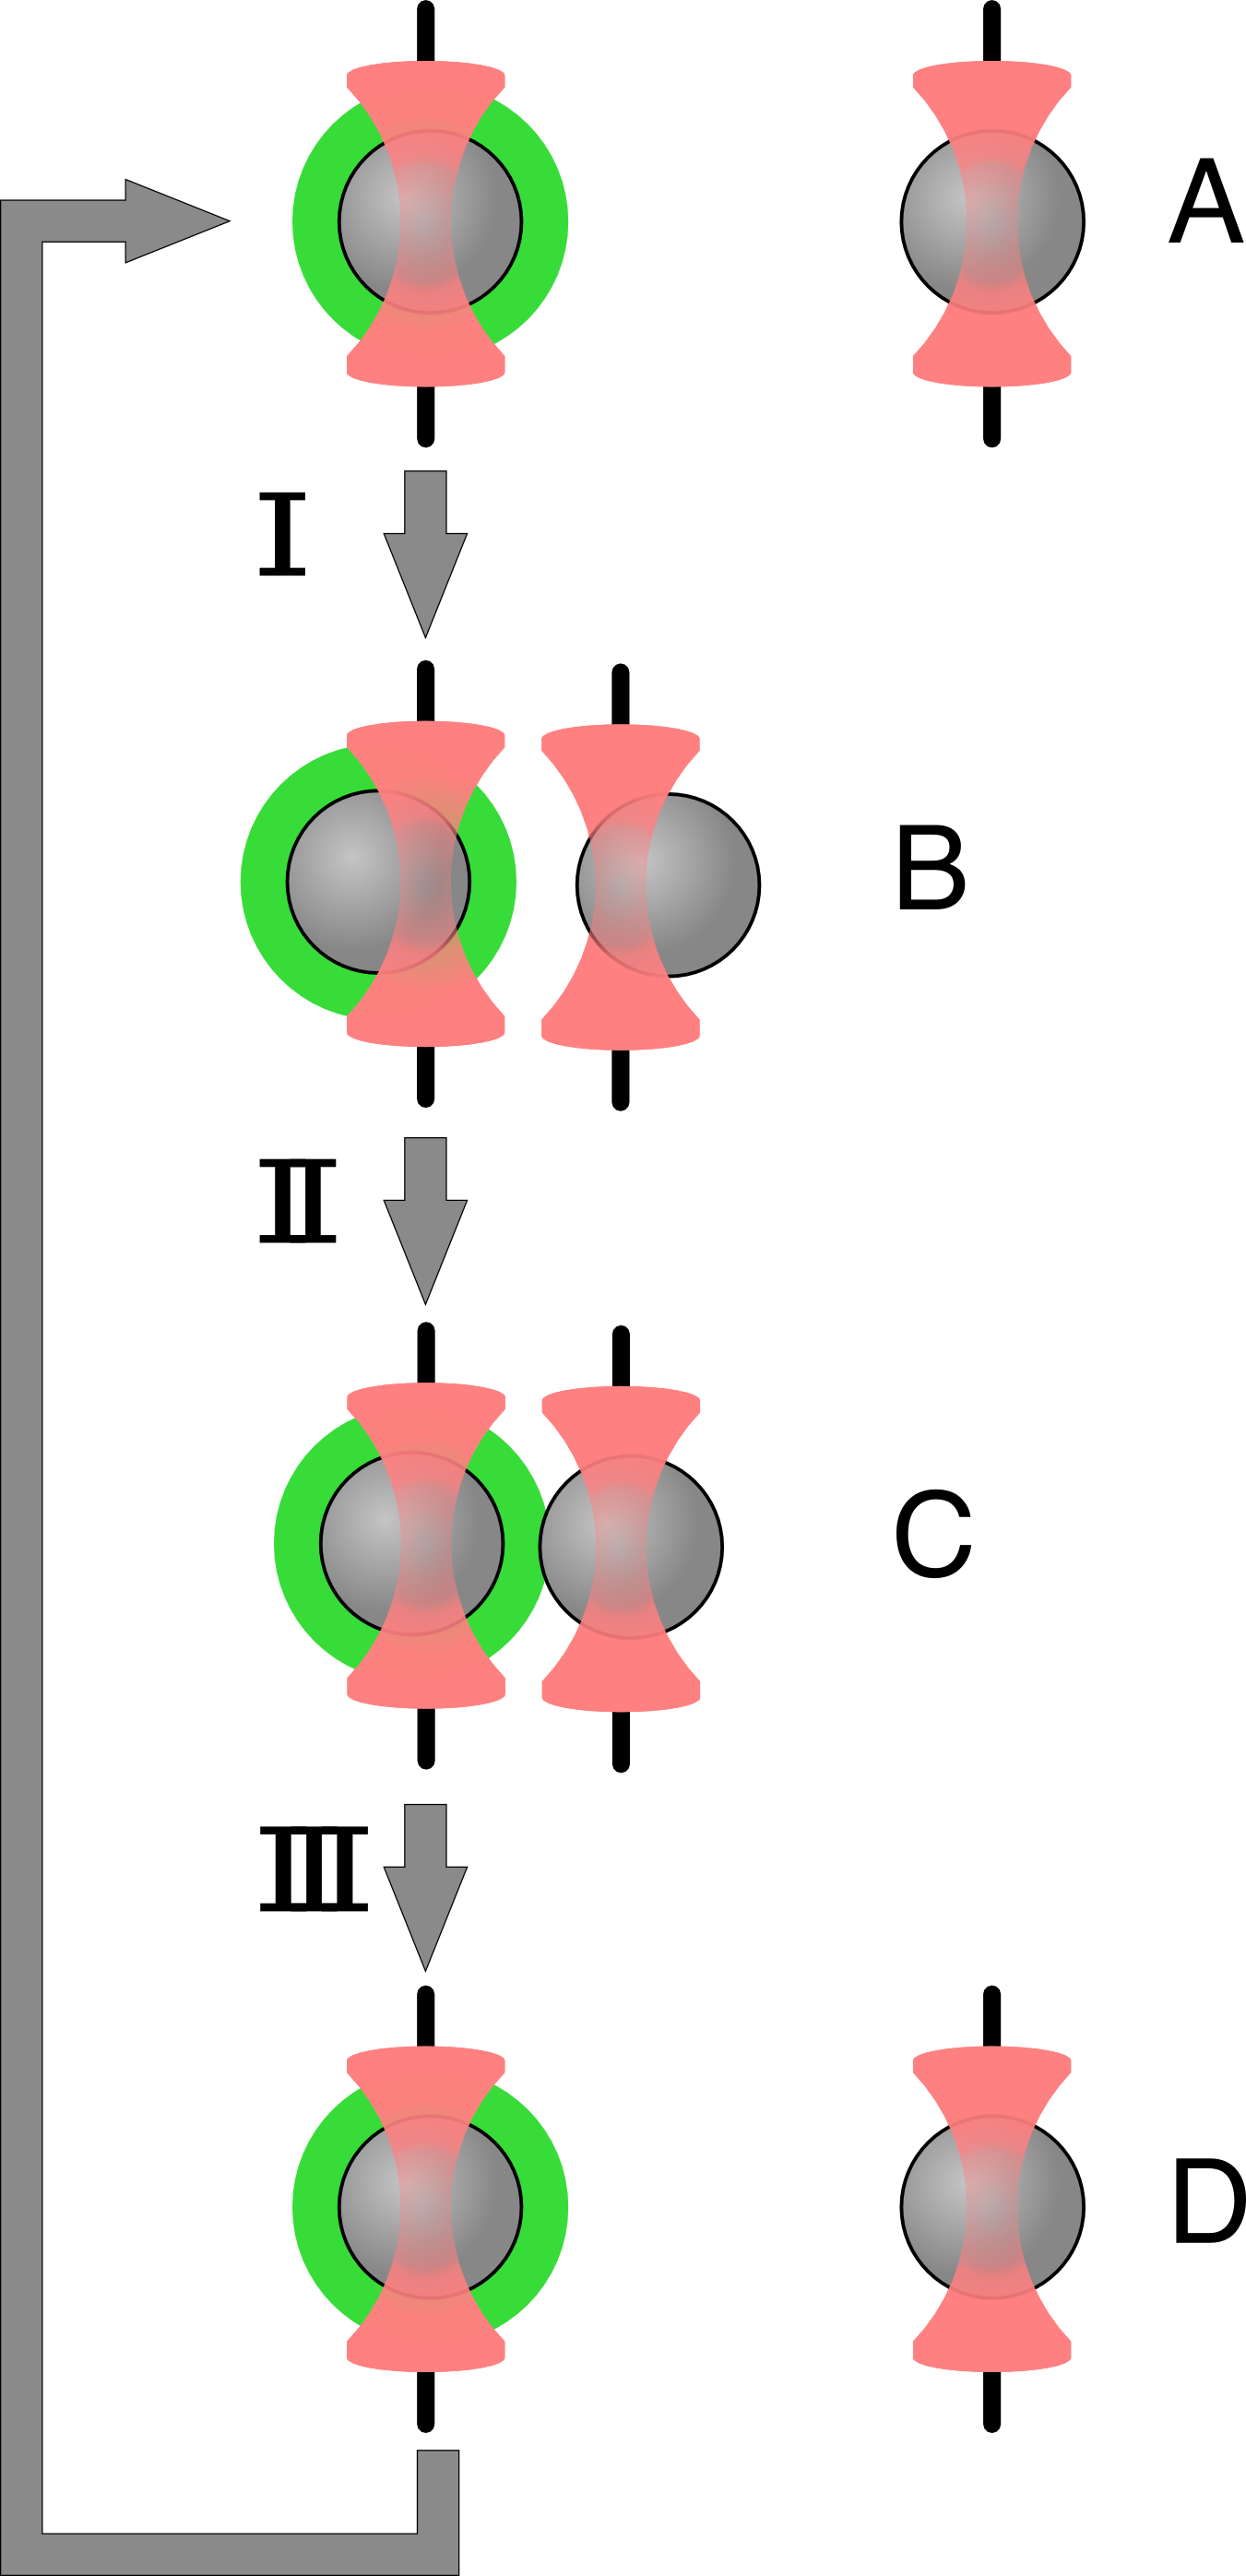
\includegraphics[width=0.500\linewidth]{beed_move.png}
\caption{Schematic of indentation experiment. On the left is the actin-bead, covered
with actin, in the static trap, on the right the probe-bead in the mobile
trap. At the beginning of the experiment (A) the probe-bead is situated far from
the actin-bead. During the approach phase (I) the moving trap approaches
the static trap at 10µm/sec until it reaches the minimal approach
distance (B). The moving trap stays at the minimal approach distance for
3sec (II), which constitutes the relaxation phase.C) The actin gels are
relaxed, the distance between bead is smaller than on B. III), the moving
trap retracts at 10 µm/sec back to its initial position.}\label{index-latex:bead-move}\end{figure}


\section{Time Shared Optical Traps}
\label{index-latex:time-shared-optical-traps}\label{index-latex:time-shared-ot}
The optical trap is built on an inverted microscope (Olympus, IX71) equipped with
a fluorescence (200W mercury lamp, Osram, Munich, Germany). The sample is observed
through an Olympus 60X water immersion objective (Olympus) with numerical aperture NA=1.2, that also
serves at the entry point of the optical tweezer laser.  The light source is
an infrared fiber laser (\(\lambda=1064nm\), YLP-1-1064, IPG,
Germany). The X, Y positionings and the trapping force stiffness are controlled
by 2 Acousto Optic Deflectors (AODs, AA-Optoelectronics, France) that are placed  in the conjugated plane of
the objective back focal plane .
Multiple traps can be achieved by switching the laser between
multiple positions within a switching time, in the order of 5 µs, and resting
on each position 20µs or more.

Light refracted by the trapped sample is collected by a 40X (N.A:0.9, Olympus)
water immersion objective, and imaged on a quadrant photodiode (QPD) conjugated
with the back focal plane of the light collection objective. Signals from the
QPD (\(\Delta X, \Delta Y\) and \(\Sigma\)) are sampled at 500kHz, by a Digital
To Analogic Aquisition card (NI PCIe-6363, National Instruments, Austin,
Texas) and controlled by a custom written Labview software (National Instruments)
coupled with Matlab (Mathworks, Natick, MA). Raw signals are preprocessed by binning all
voltages measured during the laser resting time (typically 20µs, at one position). Finally,
the mean and standard deviation for each trap visit is stored for further processing.

The trap stiffness is inferred from bead radius, laser power, number of present
traps and controlled experiment data. In controlled experiments, the trap stiffness was
calibrated using the power spectral density method, and was determined
to be as high as 80 pN/µm at full laser power (119mW) for a single trap.
In the case of multiplexing, both traps as used in this work, were calibrated before
the experiment.
The sample coarse positioning was achieved through a pair of micrometer precision
screws, capable of translating the microscope stage in X and Y, and finer positionings in X,Y and Z directions  with the help of a 3D piezo stage, with
an accessible range of 80 µm in each direction and a sub-micrometer accuracy.


\section{Oocyte}
\label{index-latex:oocyte}

\subsection{Oocyte obtention}
\label{index-latex:oocyte-obtention}
Oocyte culture, collection, and micro injection?, were done at the College de France by Maria Almonacid.

Oocytes were collected from 11 to 15 week old mice (WT), fmn2-/- as previously
described in {\hyperref[index-latex:holubcova2013]{{[}Holubcova et al. 13{]}}} and maintained in Prophase I in M2+BSA
supplemented with  1µM Milrinone. Oocyte were then injected with cRNA,  using a
micro-injector Eppendorf FemtoJet. Imaging was carried out at \(37^\circ{}C\).


\chapter{Mechanical properties of a far reaching actin cloud}
\label{index-latex::doc}\label{index-latex:mechanical-properties-of-a-far-reaching-actin-cloud}

\section{Introduction}
\label{index-latex:introduction}
We have seen that the actin cytoskeleton plays a major role in
cellular mechanics.Essential for force generation, it is a
key component for cell motility. It has also been extensively studied both in
cells and biomimetic systems.

Actin can form a variety of cells networks, ranging from dense branched
networks at the lamellipodia leading edge to bundled parallel structures
forming the filopodia.  The actin network reconstruction has been achieved in
biomimetic systems using purified components {\hyperref[index-latex:plastino2005]{{[}Plastino et al. 05{]}}},
{\hyperref[index-latex:loisel1999]{{[}Loisel et al. 99{]}}}, {\hyperref[index-latex:bernheim-groswasser2002]{{[}BernheimGroswasser et al. 02{]}}},  {\hyperref[index-latex:pontani2009]{{[}Pontani et al. 09{]}}}, and
many properties of these networks have been measured.

It has been determined that the actin cortex provides mechanical support for the
plasma membrane and that it extends over a few hundreds of nanometers.Many
cellular processes hint that actin structures connected to this cortex, are
key elements in organelle and chromosome positioning.

In this part of the manuscript, we will investigate how a sparse actin structure can
emanate from the actin cortex, and explore its properties. Through the use of the
{\hyperref[index-latex:bead-motility-assay]{\emph{bead-motility}}} (\autopageref*{index-latex:bead-motility-assay}) biomimetic system aiming at reconstituting
the actin cortex and its dendritic structure, we will show that a sparse actin filaments network
emanating from the cortex has a mechanical effect, sufficient to
displace objects of cells organelles size at distances up to tens of micrometers
away from the actin cortex.

The actin cortex branched structure underneath the plasma membrane of
cells implies a structure governed by Arp2/3. To what extend can Arp2/3 and CP be used
to form a biomimetic actin cortex has already been widely studied. In
{\hyperref[index-latex:kawska2012]{{[}Kawska et al. 12{]}}}, both \emph{in vitro} measurements on reconstituted actin cortices
on beads and simulations investigate the effect of cross-linking and
Capping Protein on the formed actin gel. It can be observed both experimentally and in
simulation that a filaments network escapes from what is defined as the actin
cortex (\hyperref[index-latex:fig-bead-tirf]{Figure  \ref*{index-latex:fig-bead-tirf}}). The effect of these long filaments is not taken into account in the
\emph{in-silico} system, where the analysis is restricted to filaments shorter than 10
µm. The effect of dense entangled actin networks generated from
randomly placed primers on the bead surface only participates in the tension increase and
contributes to symmetry breaking.
\begin{figure}[htbp]
\centering
\capstart

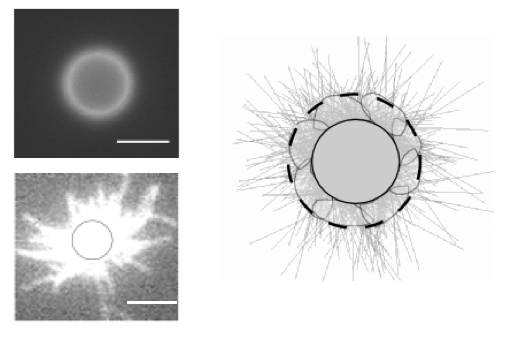
\includegraphics[width=0.700\linewidth]{Bead-tirf-fluo-sim.png}
\caption{Upper Left : Fluorescence image of an actin bead with a growing actin
cortex. Escaping filaments form the actin cloud that can  hardly  be seen
in fluorescence. Scale bar is 2 µm. Lower Left: Total Internal Reflexion
(TIRF) image of actin polymerising on an actin bead. Escaping filaments can
directly be observed. The gray circle represents the bead size.  Right :
Representation of the actin growth simulation with delimitation between the
entangled branched actin network and escaping filaments.  Adapted from
{\hyperref[index-latex:kawska2012]{{[}Kawska et al. 12{]}}}.}\label{index-latex:fig-bead-tirf}\end{figure}

The limit of the dense network, visible in epifluorescence, is defined in
{\hyperref[index-latex:kawska2012]{{[}Kawska et al. 12{]}}} by the position of the half-maximum fluorescent intensity (\hyperref[index-latex:fig-intensity-profile]{Figure  \ref*{index-latex:fig-intensity-profile}}).
The networks properties are measured by {\hyperref[index-latex:pujol2012]{{[}Pujol et al. 12{]}}} using
magnetic beads and phalloidin-stabilized actin. Though, they do not
investigate the sparse and softer actin networks that originate from the visible
part.

Using {\hyperref[index-latex:time-shared-ot]{\emph{time-shared optical tweezer}}} (\autopageref*{index-latex:time-shared-ot}) we are able to probe
the mechanics of this soft actin structure at a timescale shorter than the
characteristic time of actin polymerisation and forces in the pN range. We will show
that beyond the dense dendritic network mimicking the actin cortex, which has
been measured to have an {\hyperref[index-latex:elastic-modulus]{\emph{elastic modulus}}} (\autopageref*{index-latex:elastic-modulus}) in the order of
kPa {\hyperref[index-latex:pujol2012]{{[}Pujol et al. 12{]}}}, the soft actin cloud is much softer with
a stiffness in the Pa regime.  This might explain why such a
structure has not previously been observed with less sensitive techniques than optical
tweezers. The size of this actin cloud and its ability to sustain forces
suggest that in cells, the actin cortex is not sharply delimited and that
structures escaping from it may play a role in organelle positioning.

Hereunder are the questions we address in this part of the manuscript :
How far does the soft part of the gel extend ? What are its precise mechanical properties?  How does it change
over time?  Is the actin cloud elastic or viscous?
\begin{figure}[htbp]
\centering
\capstart

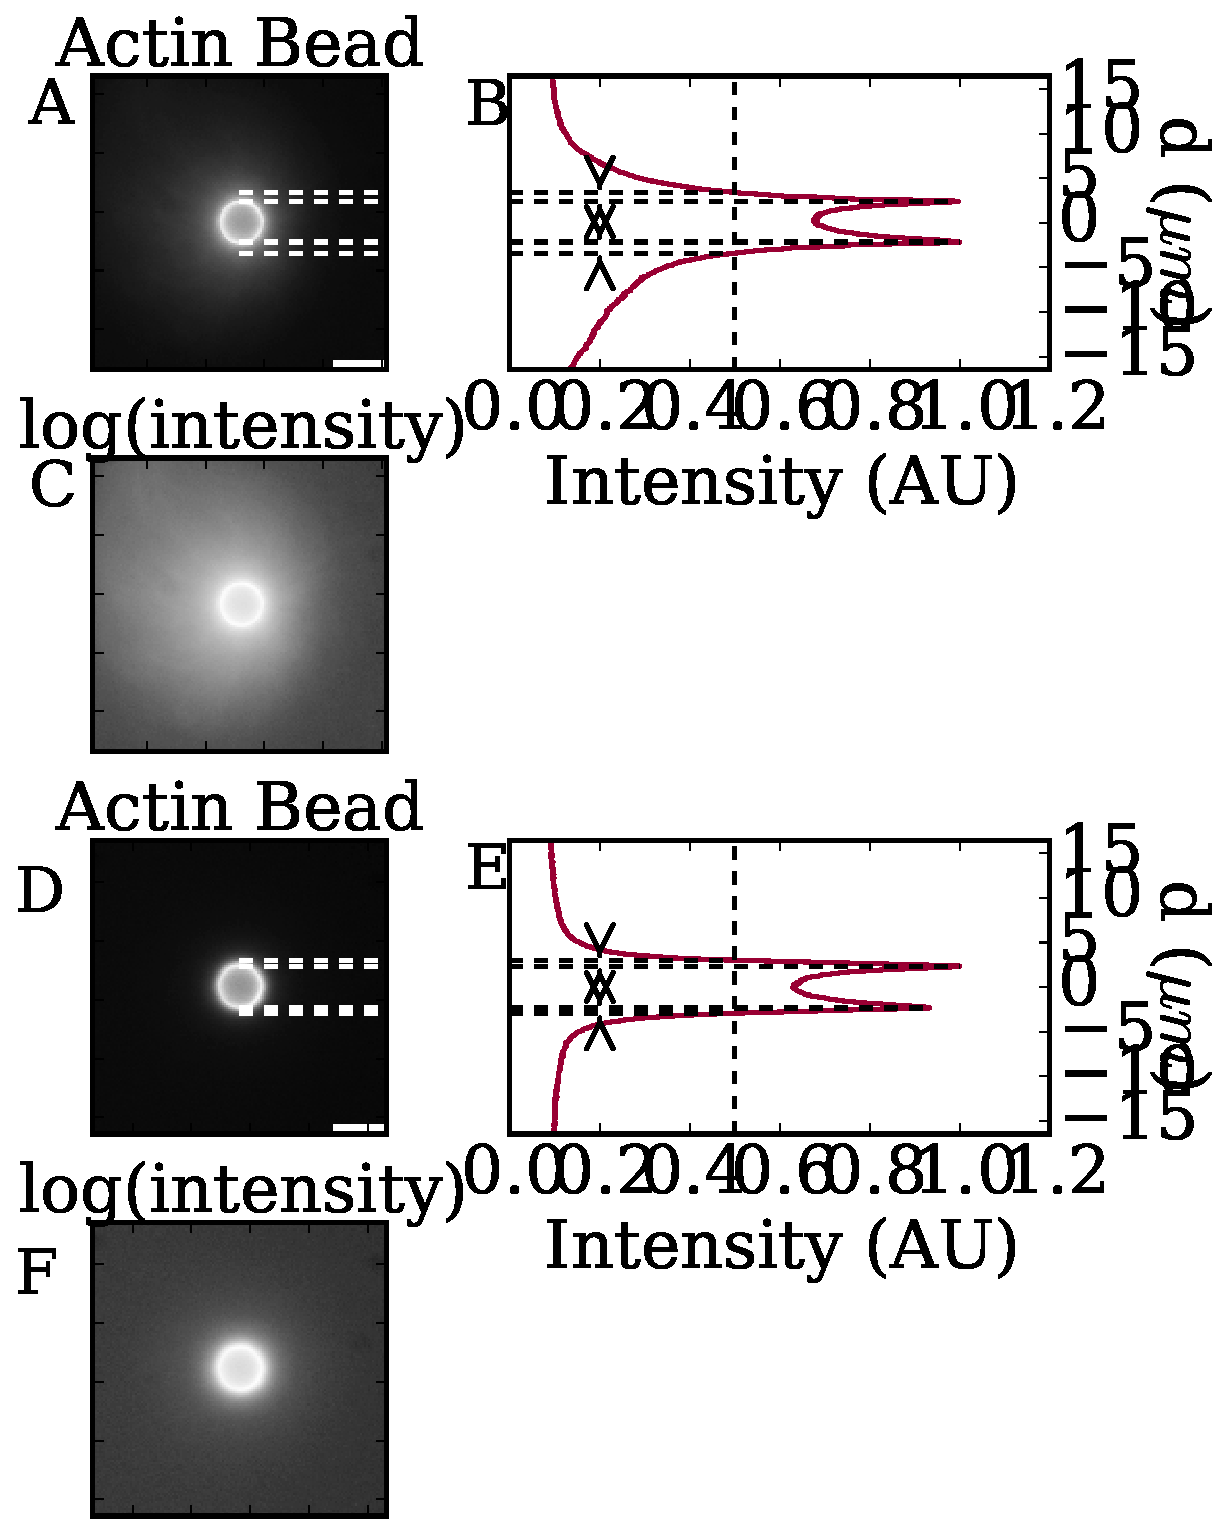
\includegraphics[width=0.800\linewidth]{intensity_profile_xnM_Arp_xnM_CP_xmin.pdf}
\caption{A) Epifluorescence image of polystyrene bead with a growing actin gel in
presence of 25 nM of Arp2/3 and 25 nM of Capping Protein. Scale bar is 5
µm.  B) Normalized intensity profile of fluorescence image with gel thickness
shown with dashed line as defined in {\hyperref[index-latex:kawska2012]{{[}Kawska et al. 12{]}}} :
Distance between maximum intensity and half-maximum intensity.  C)
Epifluorescence image of log(intensity). D,E,F) Same as A,B,C, in absence
of Capping Protein}\label{index-latex:fig-intensity-profile}\end{figure}


\section{Actin-Bead System}
\label{index-latex:actin-bead-system}
Reproducing the actin cortex and studying the mechanics of actin structures
emanating from it {\hyperref[index-latex:bead-preparation]{\emph{required 4.3 µm diameter polystyrene beads}}} (\autopageref*{index-latex:bead-preparation})
coated with a nucleation promoting factor. Theses beads were placed
in the {\hyperref[index-latex:atp-mix-buffer]{\emph{ATP mix buffer}}} (\autopageref*{index-latex:atp-mix-buffer}) in presence of 25nm of Arp2/3
complex, 4µm of monomeric actin (20\% fluorescently labeled), 12 µM profilin and
a variable amount of Capping Protein. {\hyperref[index-latex:m-et-m]{\emph{see Material and Methods}}} (\autopageref*{index-latex:m-et-m}).
These beads are referred to as actin-beads.

These conditions were chosen in order to grow a dense network on the actin-bead surface as in {\hyperref[index-latex:kawska2012]{{[}Kawska et al. 12{]}}}. We determined at an amount of 25nM ATP and a varying
amount of Capping Protein concentration in order to cover conditions where the
dense gel formed on the actin-bead was able to accumulate sufficient stress
to lead to symmetry breaking (CP between 15  and 35 nM, see part {\hyperref[index-latex:bead-motility-assay]{\emph{Bead Motility Assay}}} (\autopageref*{index-latex:bead-motility-assay})). We also investigated
conditions where the amount of Capping Protein was too low (\textless{} 15nM) or too high
(\textgreater{}35 nM) to permit symmetry breaking.

We selected a 4.3 µm bead diameter in order to get a characteristic symmetry
breaking time of 20 to 40 minutes.
A smaller bead radius implies a
faster increase of stress and a shorter symmetry breaking time.
Chosing 4.3µm provides sufficient time to proceed with the
experiments before symmetry breaking occurs.

All measurements were made on an actively growing actin network which
was not stabilized before symmetry breaking
occurred for Capping Protein concentration in the range 15 to 35 nM {\hyperref[index-latex:kawska2012]{{[}Kawska et al. 12{]}}}.


\section{Probe Bead System}
\label{index-latex:probe-bead-system}
Beside actin-bead, the experiment required a polystyrene bead passivated
with BSA. These beads are referred to as probe-beads.  The probe-bead size, similar to the actin-bead’s, ensured the optical
trapping of both beads in the same observation plane. In the case of different beads diameters, the axial forces on the beads were different. This axial
displacement of the two beads during the indentation process led to a
component along the z-axis which  eventually pushed one bead out of the trap.


\section{Experimental description}
\label{index-latex:experimental-description}
In order to probe the actin network, we trapped an actin-bead with a growing actin-network
and a probe-bead using time-shared {\hyperref[index-latex:time-shared-ot]{\emph{optical trap}}} (\autopageref*{index-latex:time-shared-ot}),  and
measured the forces on the actin-bead, using a QPD placed in the back focal plane of
the condenser ({\hyperref[index-latex:m-et-m]{\emph{material and methods}}} (\autopageref*{index-latex:m-et-m})).

Moreover, all force
recordings used for analysis were made on the static bead, in our case the actin bead, to avoid systematic errors of force measurements on the moving trap.

The indentation is a three step process (\hyperref[index-latex:figindent-time]{Figure  \ref*{index-latex:figindent-time}}):
\begin{itemize}
\item {} 
An approach phase at constant velocity 10µm/sec unless specified otherwise

\item {} 
A 3 second relaxation phase during which both traps remain static

\item {} 
A retraction phase  during which the probe trap returns to its initial position at 10µm/sec.

\end{itemize}


\subsection{Approach Phase}
\label{index-latex:approach-phase}
During the approach phase, the probe-trap will approach the actin-trap at constant speed (10 µm/s), as shown in
\hyperref[index-latex:figindent-time]{figure  \ref*{index-latex:figindent-time}} for times \(t < t_1\), and the actin-bead
will repel the probe-bead, due to the actin network growing on it. The force undergone
by the actin-bead will progressively increase during the probe-bead approach,
eventually reaching the maximum as the probe-trap reaches its nearest position
to the actin-trap. It should be noted that during this process,
the force between the beads pushes  them out of their respective trap centers.
The beads displacement in the trap remains negligible compared to the
distance between the two beads. Hence, in the following we will consider that the probe-bead speed is equivalent to the trap approach speed of 10µm/sec.


\subsection{Relaxation Phase}
\label{index-latex:relaxation-phase}
After the approach, the trap remains static for a 3 seconds relaxation phase
. The relaxation phase starts at \(t_1\) and
finishes at \(t_3\) as shown on \hyperref[index-latex:figindent-time]{figure  \ref*{index-latex:figindent-time}}. The duration of the relaxation phase is sufficient to allow the actin cloud  partial
relaxation but remains sufficiently short compared to
the actin polymerisation speed. Hence, the polymerisation is not expected to
change the network properties during indentation cycle and repetitive indentation (\hyperref[index-latex:reproc]{Figure  \ref*{index-latex:reproc}})

While the actin network relaxes, the forces between the two beads will slowly
decrease, thus leading to the beads getting closer to their trap center and
to each other. There is a slight decrease in distance during the relaxation phase, compared to the distance between beads. The force decrease as well as
the minimal change in distance between the two beads can be observed on \hyperref[index-latex:figindent-time]{Figure  \ref*{index-latex:figindent-time}}
in the middle part.
\begin{figure}[htbp]
\centering
\capstart

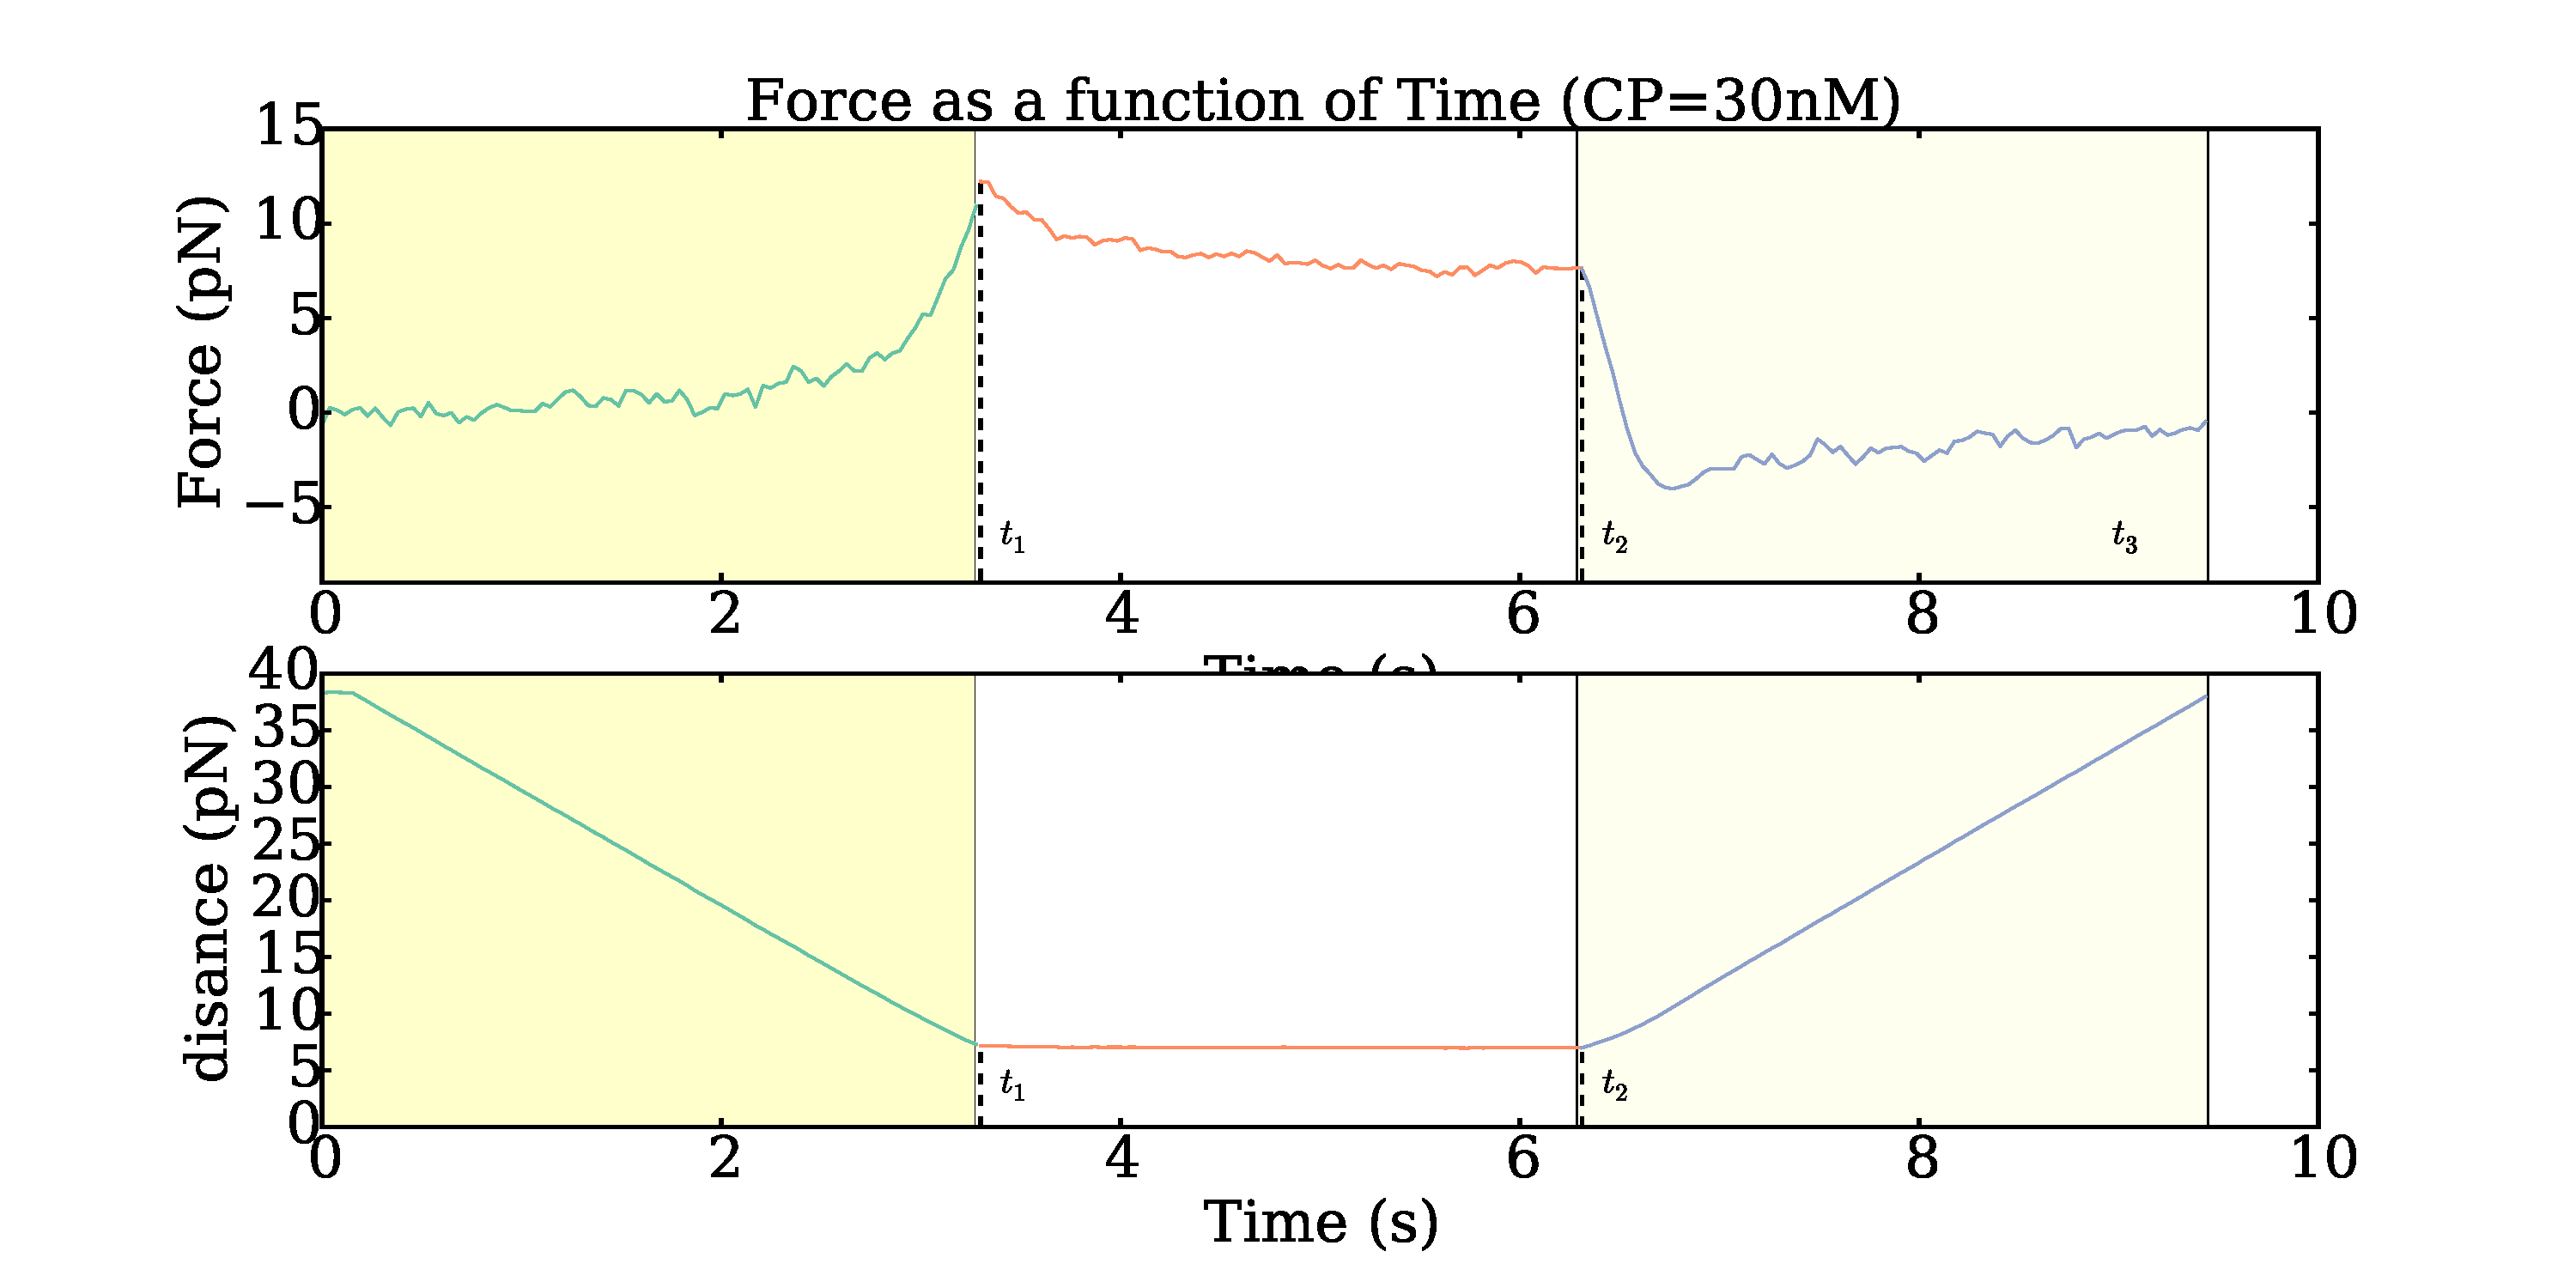
\includegraphics[width=0.700\linewidth]{force_time.pdf}
\caption{Upper graph : Force as a function of time on the actin-beads.  Lower graph
: distance between beads (distance between traps + beads
displacement from the trap center) as a function of time. The first part of each graph
(green curve, yellow back) represents the approach phase. The middle part
(orange on white) corresponds to the relaxation phase, and the right part (blue on pale
yellow) is the retraction. The observed data is a subsample of around 1 out of every
1000 acquired points. We can see on the second graph that the beads
displacement on their respective traps is negligible compared to the
trap displacement and justifies the approximation of a probe-bead
speed equivalent to the probe-trap speed.}\label{index-latex:figindent-time}\end{figure}


\subsection{Retraction part}
\label{index-latex:retraction-part}
After the three seconds of the retraction phase, the probe-trap returns to
its  initial position at 10 µm/s (\(t > t_2\)). During this phase, the force
exerted between the two beads decreases, becomes negative, reaches a minimum, and
eventually returns to zero as the probe-bead recovers its initial
position (shown on \hyperref[index-latex:figindent-time]{Figure  \ref*{index-latex:figindent-time}} right part). Negative forces
represent the forces that tend attract the two beads towards each other.


\subsection{Reconstitution of Force-distance-curve}
\label{index-latex:reconstitution-of-force-distance-curve}
The beads position in the trap as well as the force exerted on each bead can be
calculated from the position of the trap over time ( and the signal measured by the QPD. We can then recover the distance between bead centers as a function
of time.  The force-distance curve representing the force exerted by the
probe-bead on the actin-bead as a function of the distance can be computed and is
shown in \hyperref[index-latex:force-distance]{figure  \ref*{index-latex:force-distance}} where we can still distinguish the three
phases of the indentation cycle, also marked by the color used for the data.
\begin{figure}[htbp]
\centering
\capstart

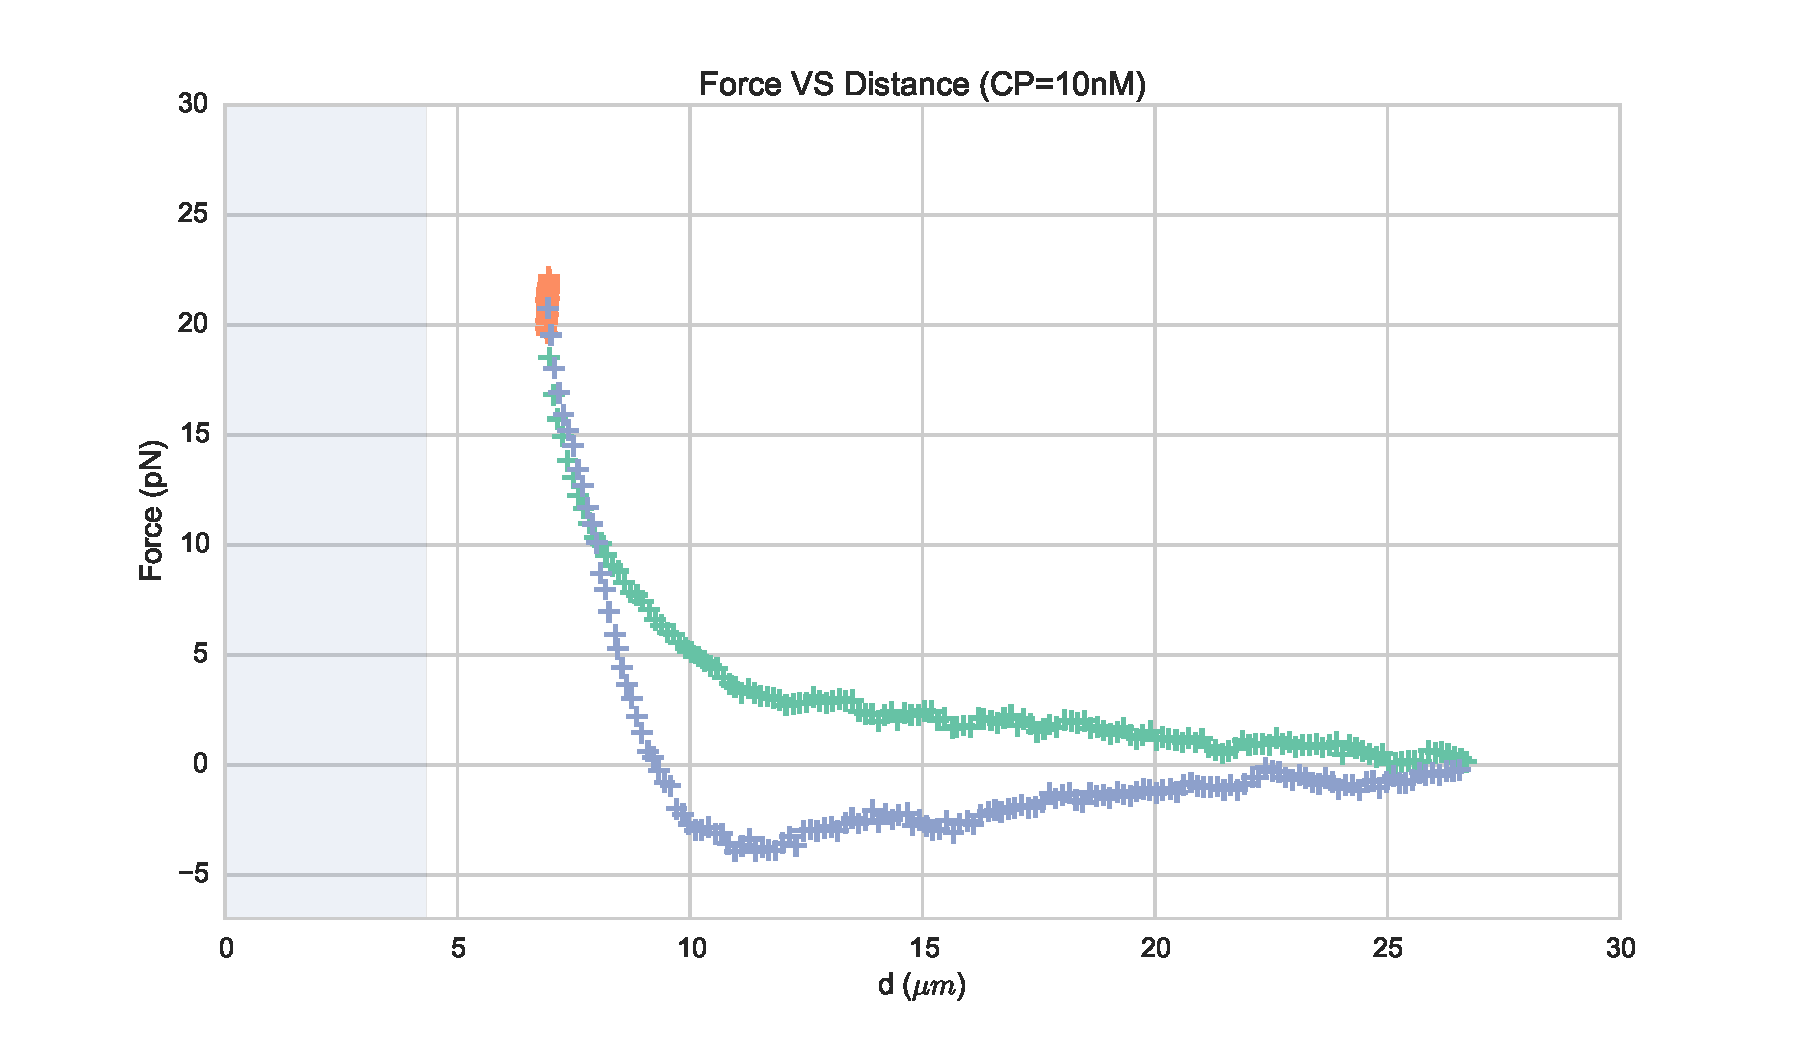
\includegraphics[width=0.800\linewidth]{force-distance.pdf}
\caption{Force exerted on the actin-bead as a function of the distance between the
two bead centers. Colors and data are the same as in \hyperref[index-latex:figindent-time]{Figure  \ref*{index-latex:figindent-time}}.
The probe-bead starts from the far right, and gets closer
while the force increases (green upper part of the curve), reaches a
maximum, and enters the relaxation phase (orange part), where the force
between both probe-beads and actin-bead decreases, while the distance  also
slightly decreases. During the retraction part (blue), the force rapidly
decreases and  reaches negative values as   the bead returns to its initial
position. The observed data is a subsample of 1 in every 1000 points of acquired
data. Shaded regions represent areas where the two polystyrene beads should
interpenetrate.}\label{index-latex:force-distance}\end{figure}


\subsection{Repetitive indent}
\label{index-latex:repetitive-indent}
The indentation cycle can be repeated several times every few seconds, to check for reproducibility and non-plastic deformation of the network after
indentation. As the network is constantly growing during the measurement, this
repeat also allows to check for possible changes of the network properties, due to actin
polymerisation. The force-distance plot is shown in \hyperref[index-latex:reproc]{figure  \ref*{index-latex:reproc}} \hyperref[index-latex:reproc-time]{,  \ref*{index-latex:reproc-time}}.
\begin{figure}[htbp]
\centering
\capstart

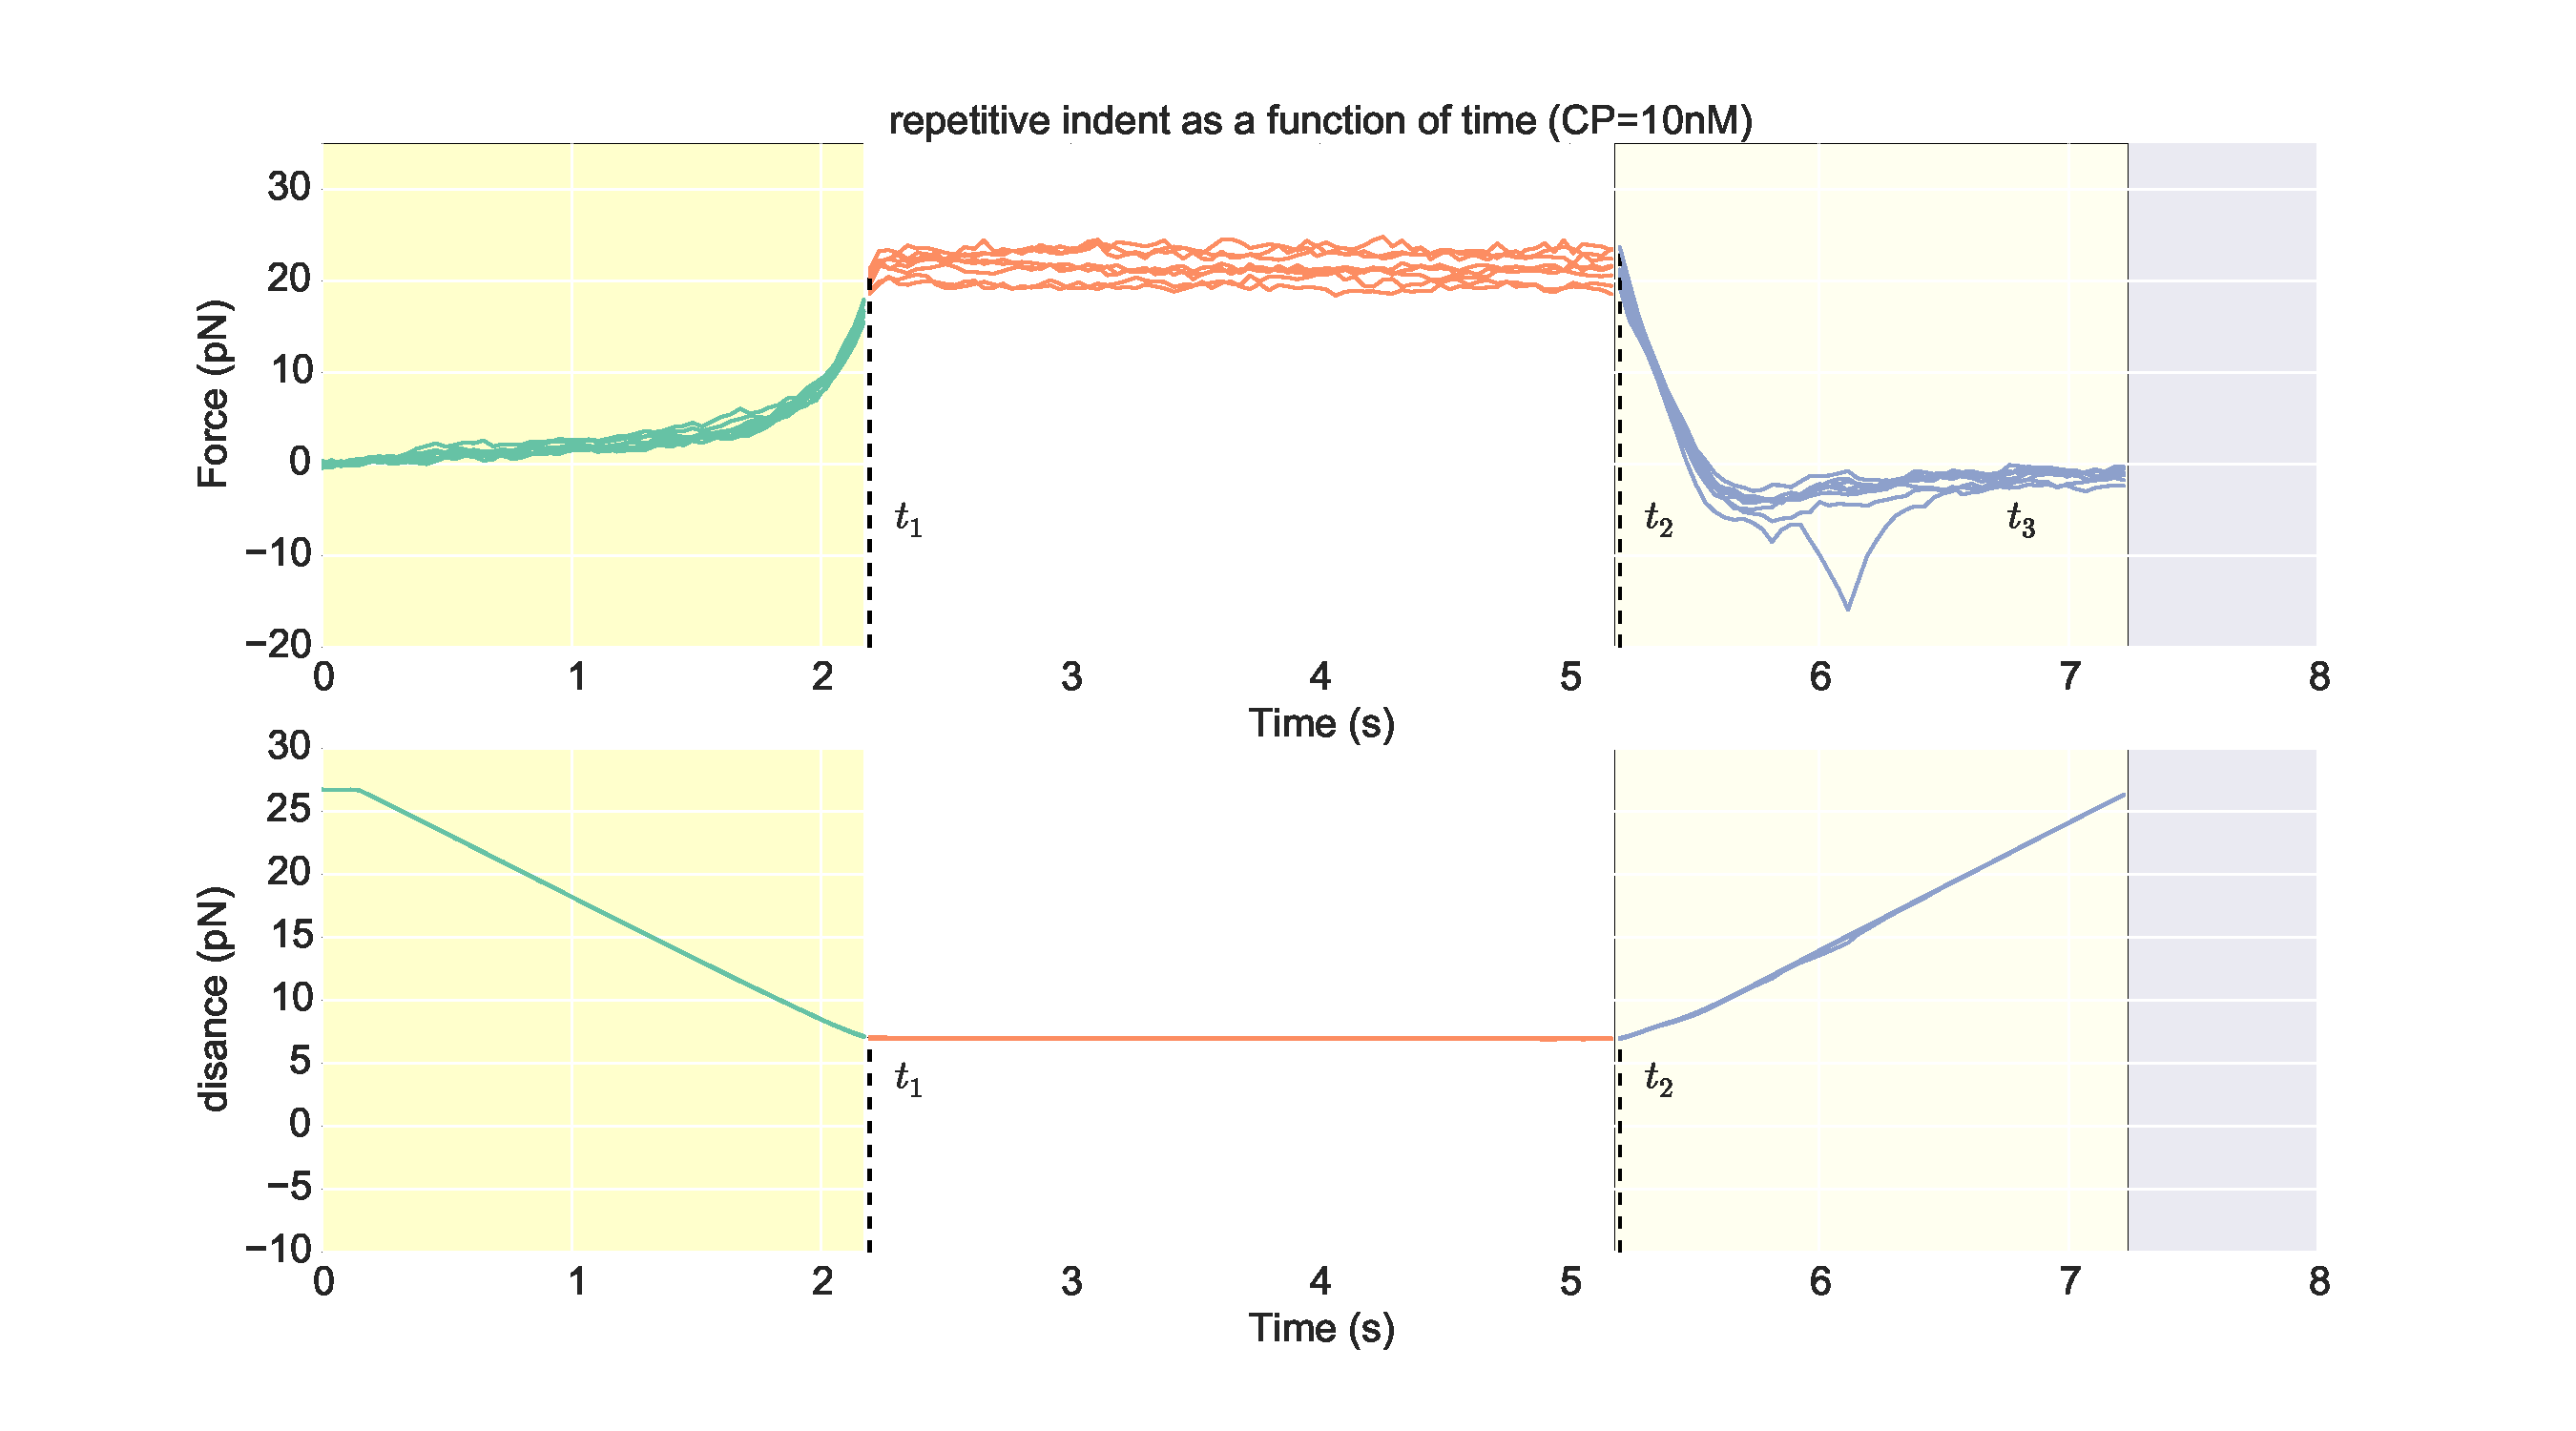
\includegraphics[width=1.000\linewidth]{reproc-time.pdf}
\caption{Upper graph : Force exerted on actin-bead as a function of time for ten
repetitive indents. In one of the cycles, a sticking event can be dentified in the
retraction phase, 6 seconds after the beginning of the cycle. Lower graph:
Distance as a function of time for  ten repetitive indents. The ten curves
can hardly be distinguished from one another, which shows the
reproducibility of indentation curves.}\label{index-latex:reproc-time}\end{figure}
\begin{figure}[htbp]
\centering
\capstart

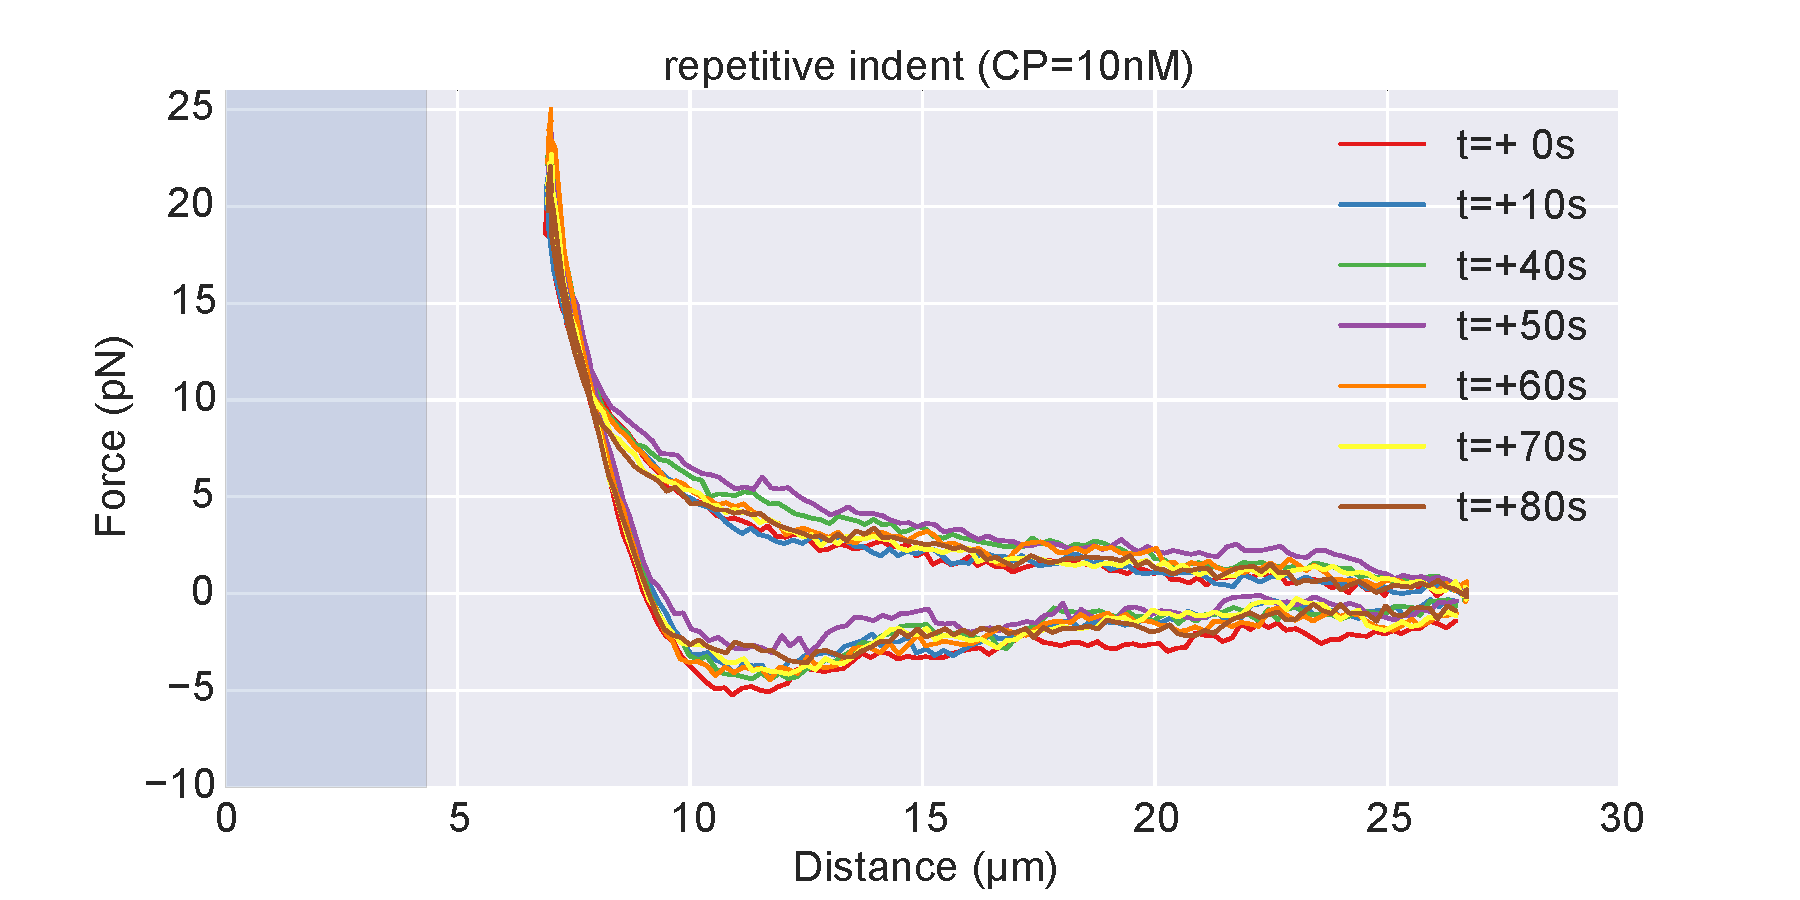
\includegraphics[width=0.800\linewidth]{reproc.pdf}
\caption{Figure showing the indentation process reproducibility on a bead with
25nM Arp2/3 and 10nM CP Subset of data from \hyperref[index-latex:reproc-time]{Figure  \ref*{index-latex:reproc-time}} highlighted
with different colors to represent the evolution of the indentation curve
over time.  Time is relative to the first indentation. Shaded areas represent
zones where the two beads should  interpenetrates.}\label{index-latex:reproc}\end{figure}


\subsection{Effect of approach speed}
\label{index-latex:effect-of-approach-speed}
{\hyperref[index-latex:gardel2003]{{[}Gardel et al. 03{]}}} suggests that, for frequencies higher than 0.1 Hz, the force due to
the actin network viscous behavior can be in the same order as the one due to the elastic
component . In order to test whether such a relaxation effect is important, we measured the effect of the
approach speed on the force measurements. \hyperref[index-latex:many-speed]{Figure  \ref*{index-latex:many-speed}} presents the
indentation speed affecting the measurement by varying the approach speed from 10
to 30 µm/s on the same actin-bead.
\begin{figure}[htbp]
\centering
\capstart

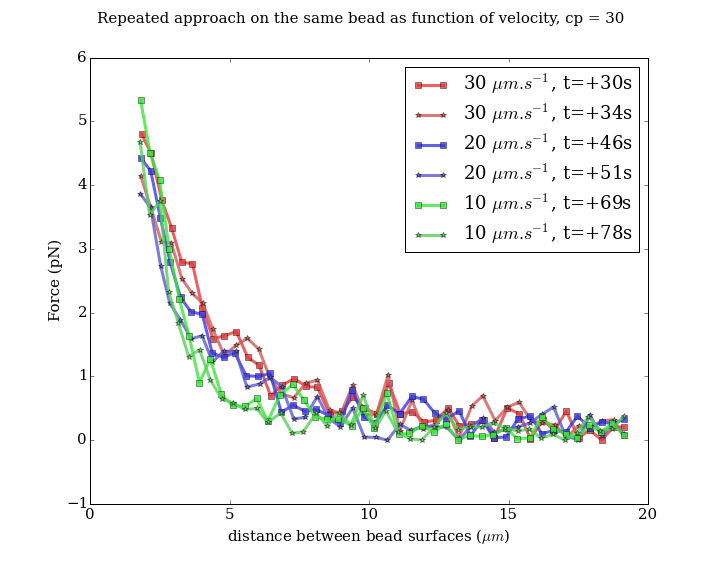
\includegraphics[width=0.600\linewidth]{many_speed.png}
\caption{Approach phase of repetitive indents at multiple speeds on the same
actin-bead. The approach phase in the different conditions is similar,
hinting at  a negligible effect of the viscosity  in the actin cloud at the
considered speed.}\label{index-latex:many-speed}\end{figure}


\section{Experimental observations}
\label{index-latex:experimental-observations}
Through the use of the bead system, we are able to reconstruct actin cortices \emph{in vitro} and
to investigate the mechanical properties inaccessible to other microscopy
techniques like TIRF. Beyond the visible actin cortex, we can detect the
presence of an actin structure with mechanical effects starting at
distances of \(> 10\mu{}m\), hence far beyond the thickness of the actin cortex (\textasciitilde{}1µm).
\hyperref[index-latex:cloud-repelling]{Figure  \ref*{index-latex:cloud-repelling}} presents a video qualitatively showing that the actin cloud growing
on actin-beads is able to repel free floating probe-beads, before they reach the
visible reconstituted cortex.

In order to quantify the distance at which the probe-beads start to be affected by the actin-cloud,
we measured the experimental noise by studying the fluctuations of the trapped probe-bead.

During the indentation, we defined \(d_0\) as the distance at which the
average force received by the probe-bead is higher than the experimental noise.
Typically the standard deviation is 2pN.

The repartition of \(d_0\) with the concentration of Capping Protein is
plotted in \hyperref[index-latex:d0-violin]{figure  \ref*{index-latex:d0-violin}}.
\begin{figure}[htbp]
\centering
\capstart

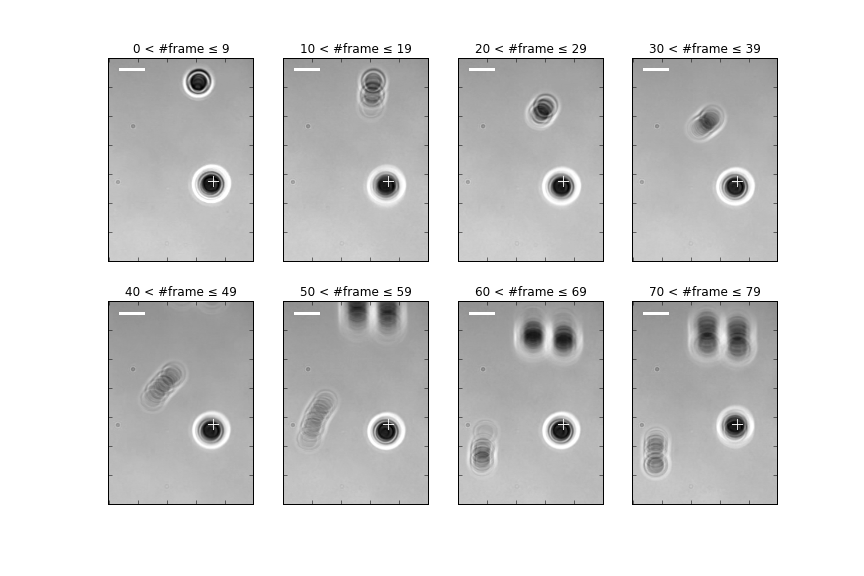
\includegraphics[width=0.850\linewidth]{cloud-repelling.png}
\caption{Chronophotography representing the displacement of a trapped actin bead in a
solution including probe-beads. During this experiment, the actin bead is kept
static in the optical trap (marked by the cross) while the stage is moved.
Scale bar is 5 micrometers. The total movie duration is 21 seconds.}\label{index-latex:cloud-repelling}\end{figure}
\begin{figure}[htbp]
\centering
\capstart

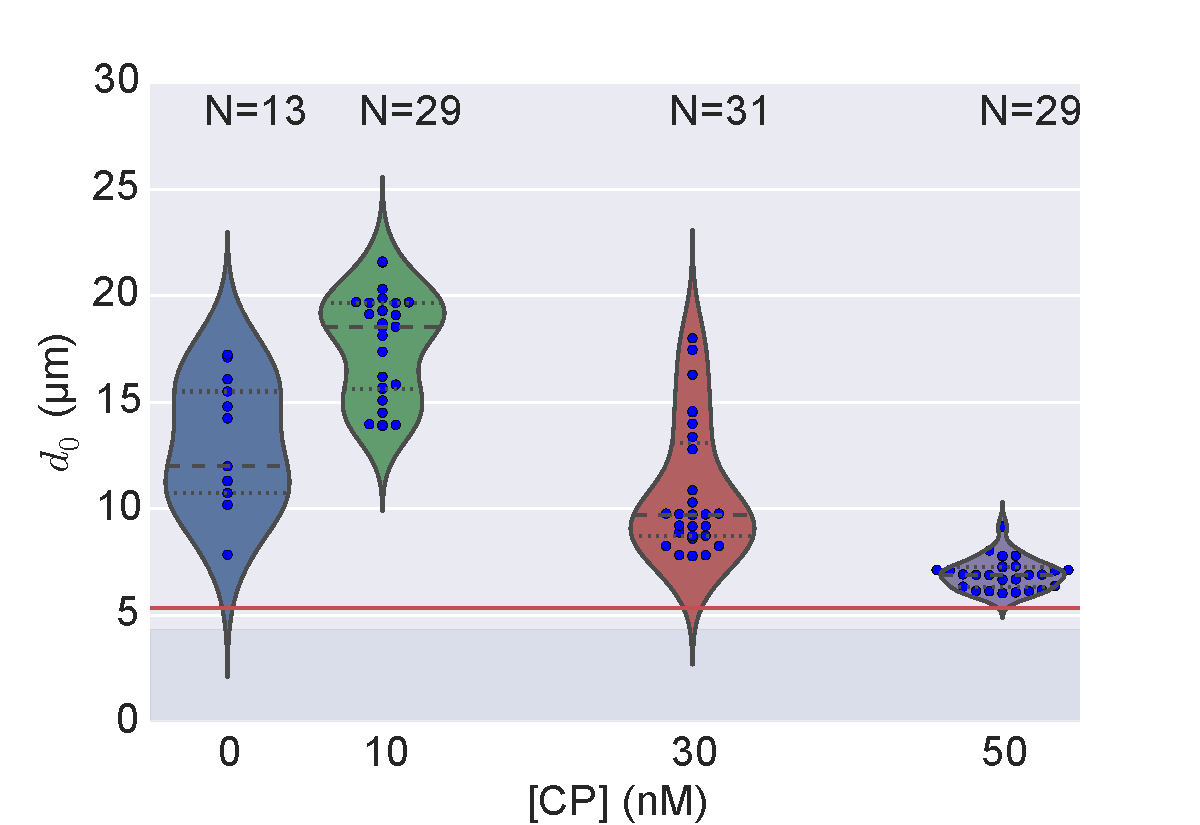
\includegraphics[width=0.650\linewidth]{d0_violin.pdf}
\caption{Repartition of the bead-center distance at which the actin cloud exerts a
force higher than the noise (\(d_0\)) on the probe-bead, as a function of
Capping Protein. The shaded region represents the bead surface position     (4.34 µm) and the red line represents the bead surface+1µm (upper bound for
the in vitro
Capping Protein concentration). The shaded region represents the bead surface position(4.34 µm) and the red line represents the bead surface+1µm
(upper bound for the in vitro
reformed actin cortex measured in {\hyperref[index-latex:kawska2012]{{[}Kawska et al. 12{]}}}). We can see in this graph that for symmetry breaking
conditions (CP 10 nM and 30 nM, the distance at which the actin cloud starts to apply
forces on the probe-bead is larger than the thickness of the actin
cortex. The distance at which the probe-bead is able to detect the presence
of the actin cloud decreases when increasing the concentration of the Capping
Protein that restricts  the actin filament growth. The condition in the absence
of Capping Protein is a particular case, as no dense actin network forms
on the surface of the actin bead.}\label{index-latex:d0-violin}\end{figure}


\subsection{Approach phase modeling}
\label{index-latex:approach-phase-modeling}
We
decided to model each part (approach, relaxation and retraction) independently, to extract their mechanical properties, by using the three phases of the experiment.
In particular, we fitted the force-distance curve of the approach phase using a power
law with 3 fit parameters \(\alpha, \beta, \delta\):
\phantomsection\label{index-latex:equation-eqa31}\begin{gather}
\begin{split}F(d) = \beta \times \left(d-\delta\right)^\alpha\end{split}\label{index-latex-eqa31}
\end{gather}
in which \(F\) represents the force exerted on the probe-bead, and \(d\)
is the distance between bead centers. The power law exponent \(\alpha\) is
expected to be negative as the force decreases with the distance \(d\), and
to characterize how fast the force increases as the two
beads approach each other. The prefactor \(\beta\) acts as a scaling factor of the
force. The offset parameter \(\delta\) shifts the curve on the distance
axis. This phenomenological model presents the particularity that the force on the probe bead tends to
\(+\infty\) when the distance \(d\) gets  to \(\delta\). The force
is undefined for values of \(d< \delta\). Hence, the offset distance \(\delta\)
practically describes the distance at which the optical trap is no longer able to
indent the network.

In the case of a hard sphere, the value of \(\alpha\) would tend towards
\(-\infty\) leading to a infinite force increase at the contact between the
two hard-spheres of same diameter, and a value of \(\delta\) equal to the
diameter of the hard sphere.  In this case \(F(d>\delta)=0\) and
\(F(d<\delta)=\infty\)

The used optical tweezer being able to apply forces up to 20pN, and the beads
having a diameter of 4.34µm , we hence determined a cross-sectional surface of roughly \(14.7\mu{}m^2\). Before
escaping the trap, the probe-bead did move up to 1µm from its
trap center. To estimate the maximal stiffness acchievable, we considered that we could
provide a clear measure of deformation in the order of 1/10 of µm,  this
leading to a maximum detectable Young's modulus of :
\phantomsection\label{index-latex:equation-eqa32a}\begin{gather}
\begin{split}E_{max} &\sim \frac{F_{max}L_{0,max}}{A_0.\Delta L} \\
        &\sim \frac{50.10^{-12} \times 1.10^{-5} }{  (\pi\times 2.17\times 10^{-6})^2 \times 1.10^{-7}              }\\
        & \sim 300 Pa\end{split}\label{index-latex-eqa32a}
\end{gather}
Any material with a stiffness much higher than 300 Pa can be considered as
infinitely rigid.

The elasticity of dense actin gels around polystyrene beads has been measured
in {\hyperref[index-latex:pujol2012]{{[}Pujol et al. 12{]}}} and found to be in the order of kPa.  Therefore, the
optical tweezers are not able to probe the mechanics of the dense gel on the
bead surface. The value of \(\delta\)  is expected to be \(> 4.34 \mu{}m\) as it partially includes the dense actin gel.

The model can be fitted independently on each experimental
approach phase. An example of such a fit is shown in
\hyperref[index-latex:force-distance-fit]{figure  \ref*{index-latex:force-distance-fit}} and the fit quality can be measured by the
coefficient \(R^2\) which has a media value of \emph{0.97}
across all fits.
\begin{figure}[htbp]
\centering
\capstart

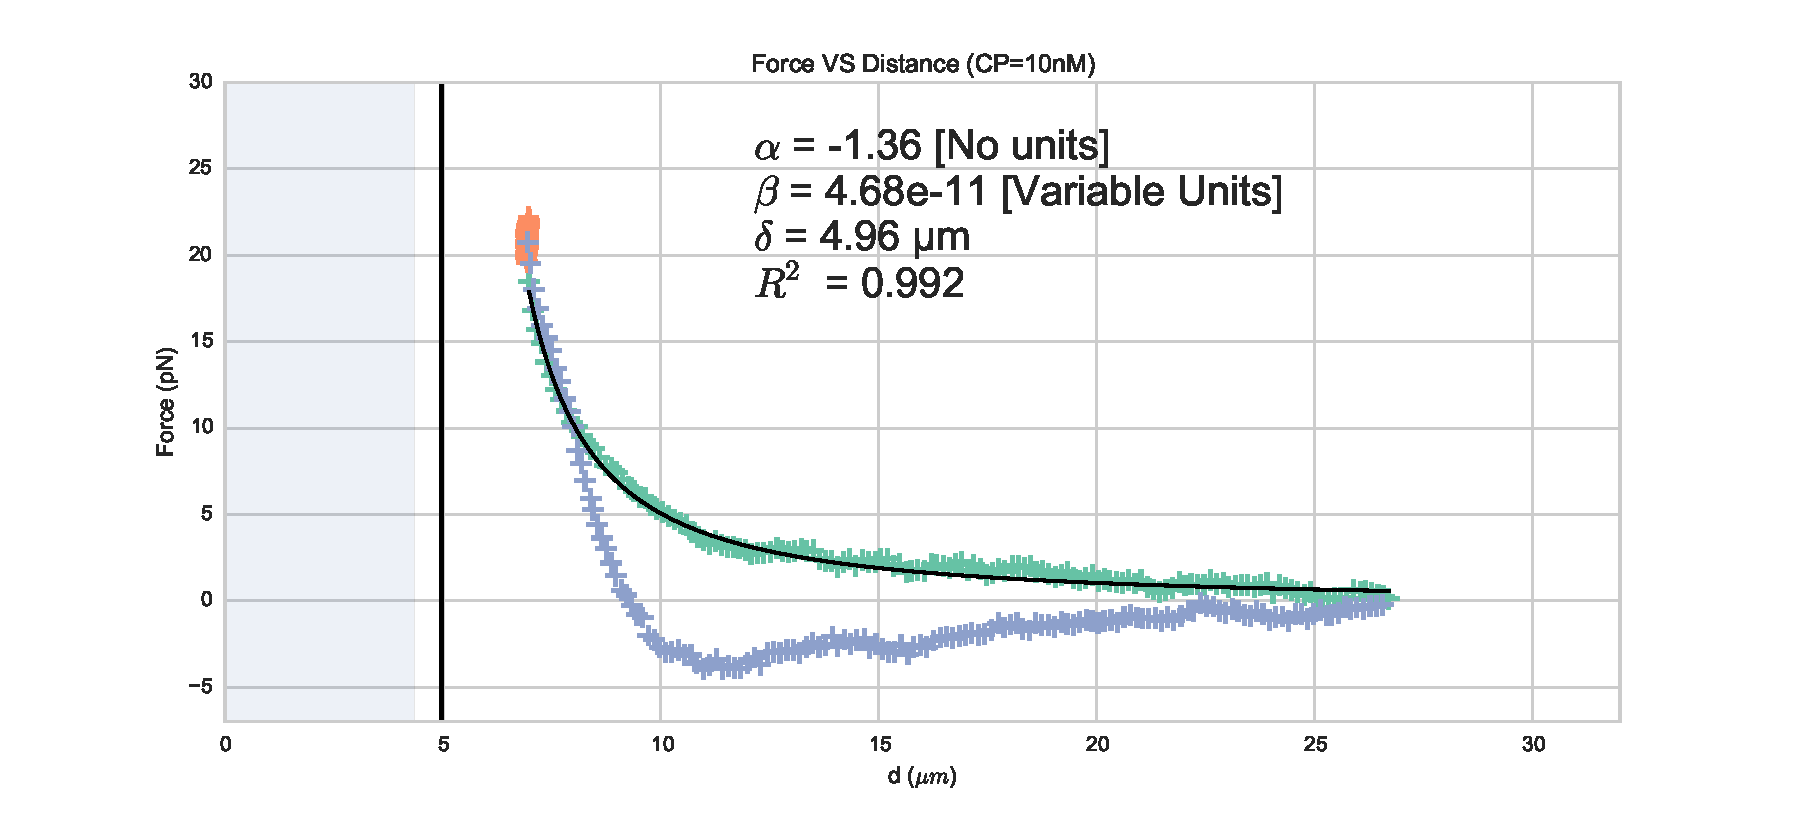
\includegraphics[width=1.000\linewidth]{force-distance-fit.pdf}
\caption{Power law model fitted on the approach phase data for one experiment in the
presence of {[}CP{]}=10nM, with the particular values found for the fit
parameters.  The vertical line represents the point where the model
diverges and the force goes to infinity, that is to say \(\delta\). The
shaded region corresponds to the distance at which the two beads should
interpenetrate. Relaxation (orange) and retraction (blue) data are not fitted.}\label{index-latex:force-distance-fit}\end{figure}

The approach phase data can be corrected for the distance offset \(\delta\)
and plot in a log-log scale allowing for a better appreciation of the fit
result (\hyperref[index-latex:force-distance-log-log]{Figure  \ref*{index-latex:force-distance-log-log}}). The corrected distance is noted with  \emph{c} indices \(d_c = d-
\delta\). In the model the force tends to infinity at \(d_c = 0\).
\begin{figure}[htbp]
\centering
\capstart

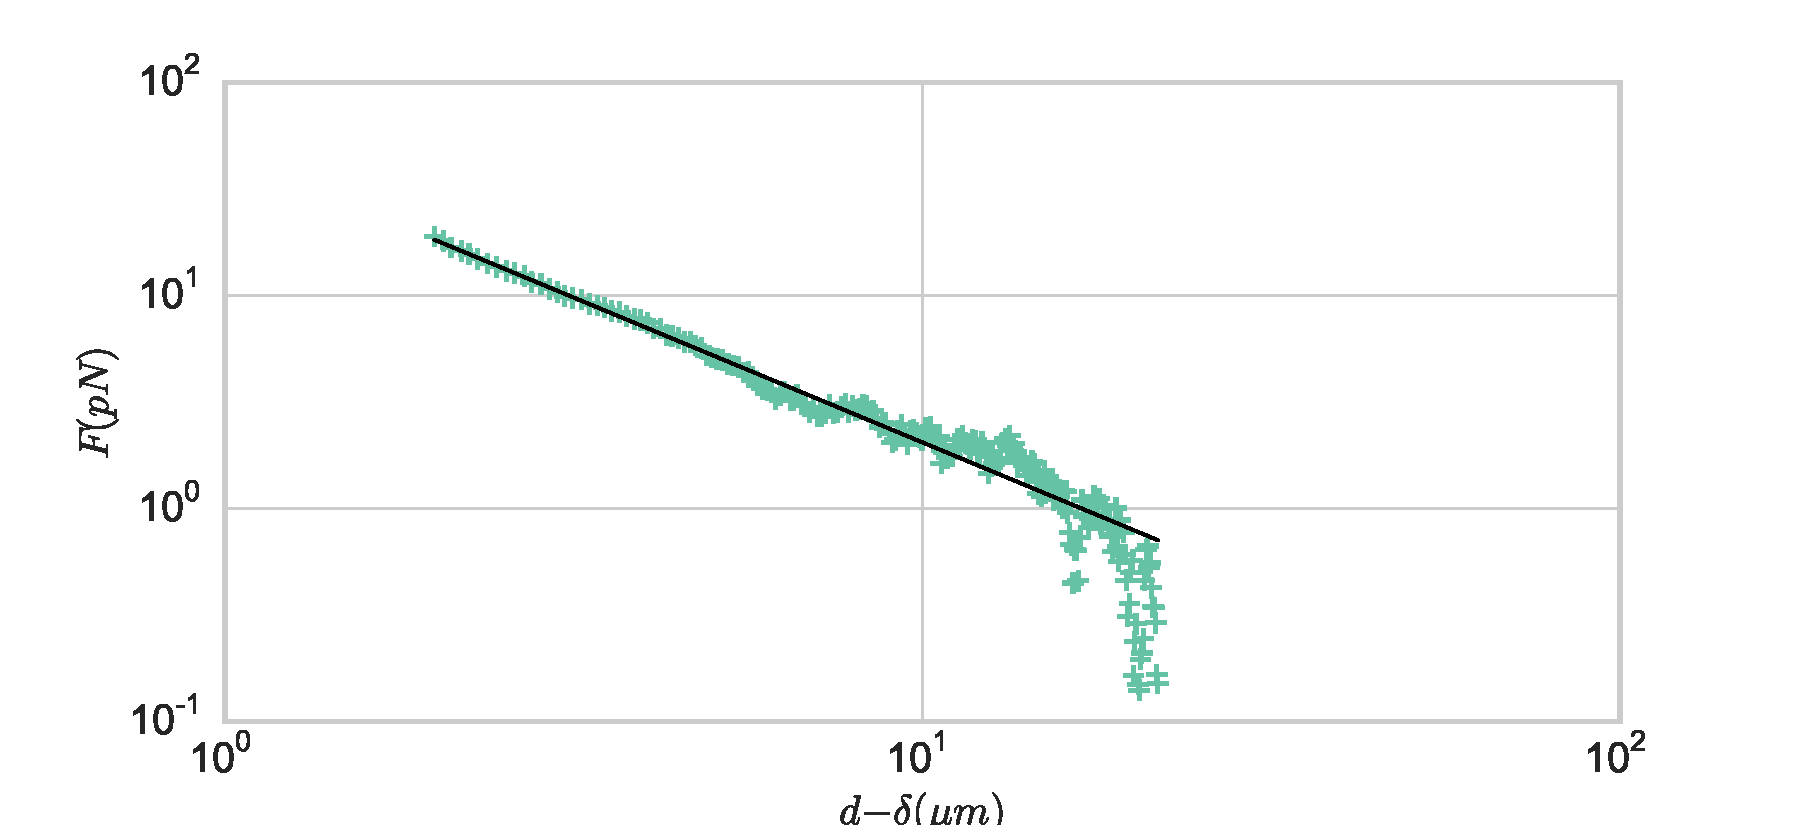
\includegraphics[width=0.800\linewidth]{force-distance-fit-loglog.pdf}
\caption{Force on the actin bead  during the approach phase as a function of bead distance
minus distance offset \(\delta\) plotted on a log-log scale. Black line
represents the power law model with the offset distance correction. Same
data as \hyperref[index-latex:force-distance]{Figure  \ref*{index-latex:force-distance}} but showing only the approach phase.}\label{index-latex:force-distance-log-log}\end{figure}

In our experiments, the polystyrene beads have an average diameter of 4.34 µm,
thus we expect \(\delta\) to be higher than the bead diameter, since the beads cannot interpenetrate.  Data with
\(\delta\) values lower than 4.34 µm (21 out of 127) are considered as
unphysical and removed from further analysis.

As expected, we found negative values for \(\alpha\). Surprisingly, the value
of alpha does not vary significantly when comparing experiments with different
amounts of Capping Protein and remains close to -1, with a mean value of -1.10, and
a standard deviation of 0.38. The distribution of the power law exponent can be
seen on \hyperref[index-latex:power-law-exponent]{figure  \ref*{index-latex:power-law-exponent}}
\begin{figure}[htbp]
\centering
\capstart

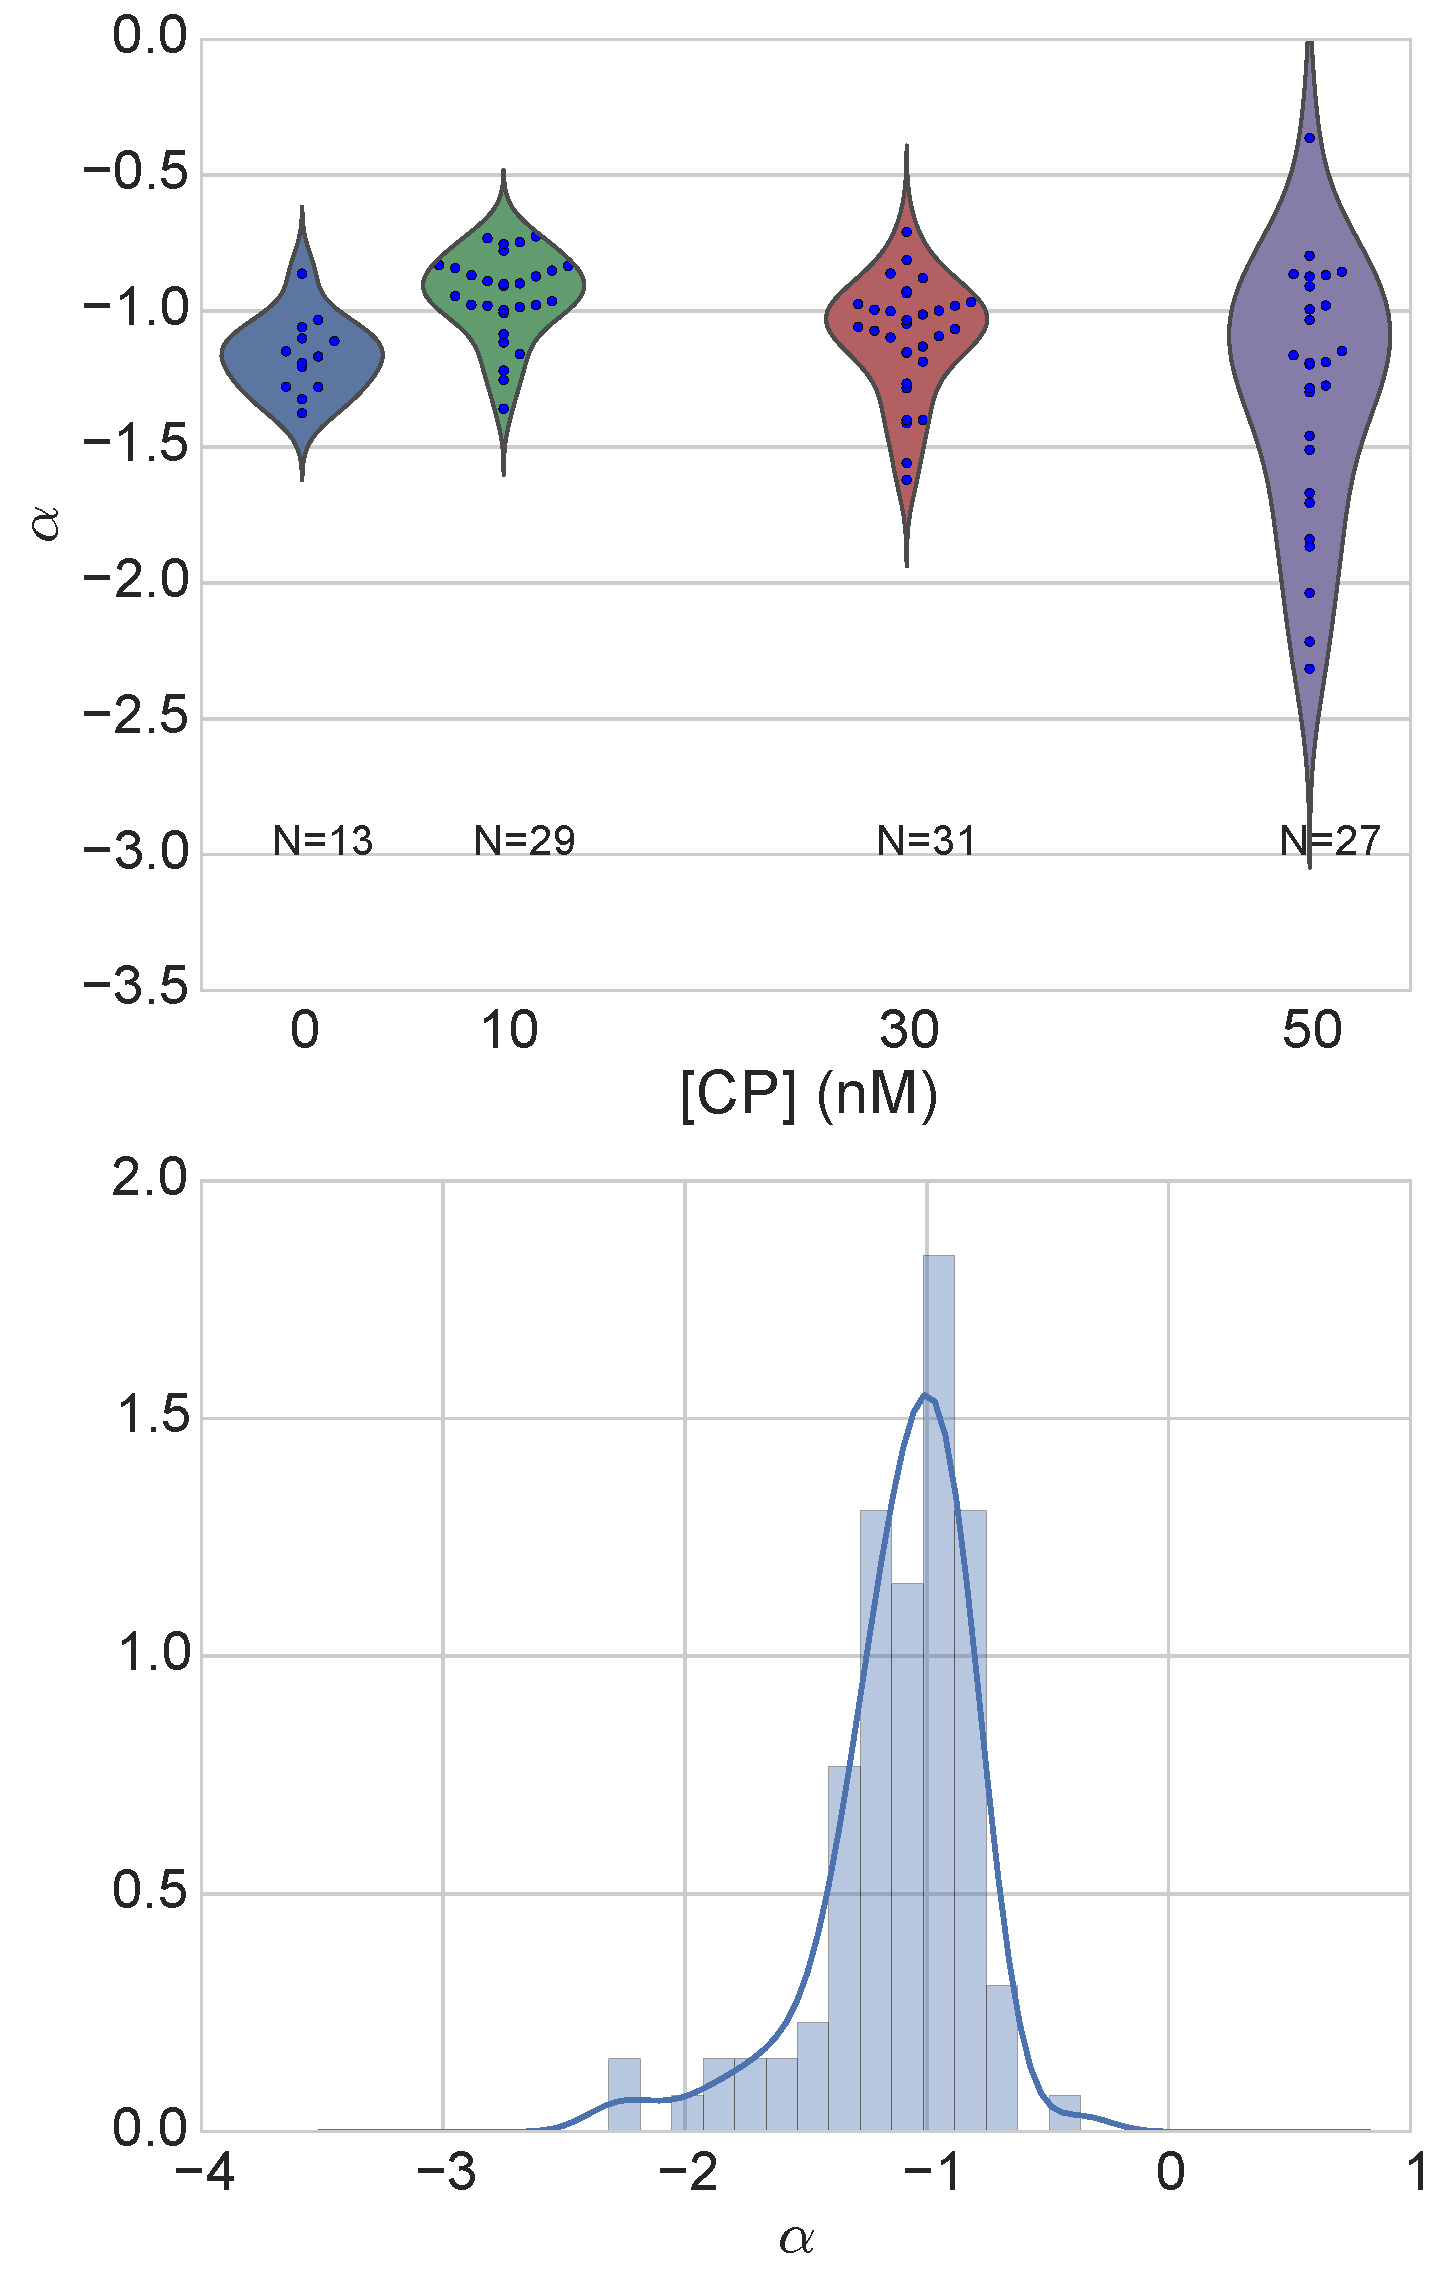
\includegraphics[width=0.600\linewidth]{alpha_violin.pdf}
\caption{Right : Violin plot showing the repartition of power law exponents as a function of concentration in Capping Protein. Left: distribution of power law exponent
\(\alpha\) regardless of the concentration in Capping Protein. Value of
exponent lies close to \emph{-1}.}\label{index-latex:power-law-exponent}\end{figure}

Due to the scale invariance of the inverse power law found above,  all the
approach phases data can be rescaled into a single master-curve (\hyperref[index-latex:fig-rescale-powerlaw]{Figure  \ref*{index-latex:fig-rescale-powerlaw}}). This is achieved
by dividing the force by the maximum force \(F_{max}\) reached during the
approach, and rescaling the distance by the minimum approach distance from which
\(\delta\) is subtracted.
\begin{figure}[htbp]
\centering
\capstart

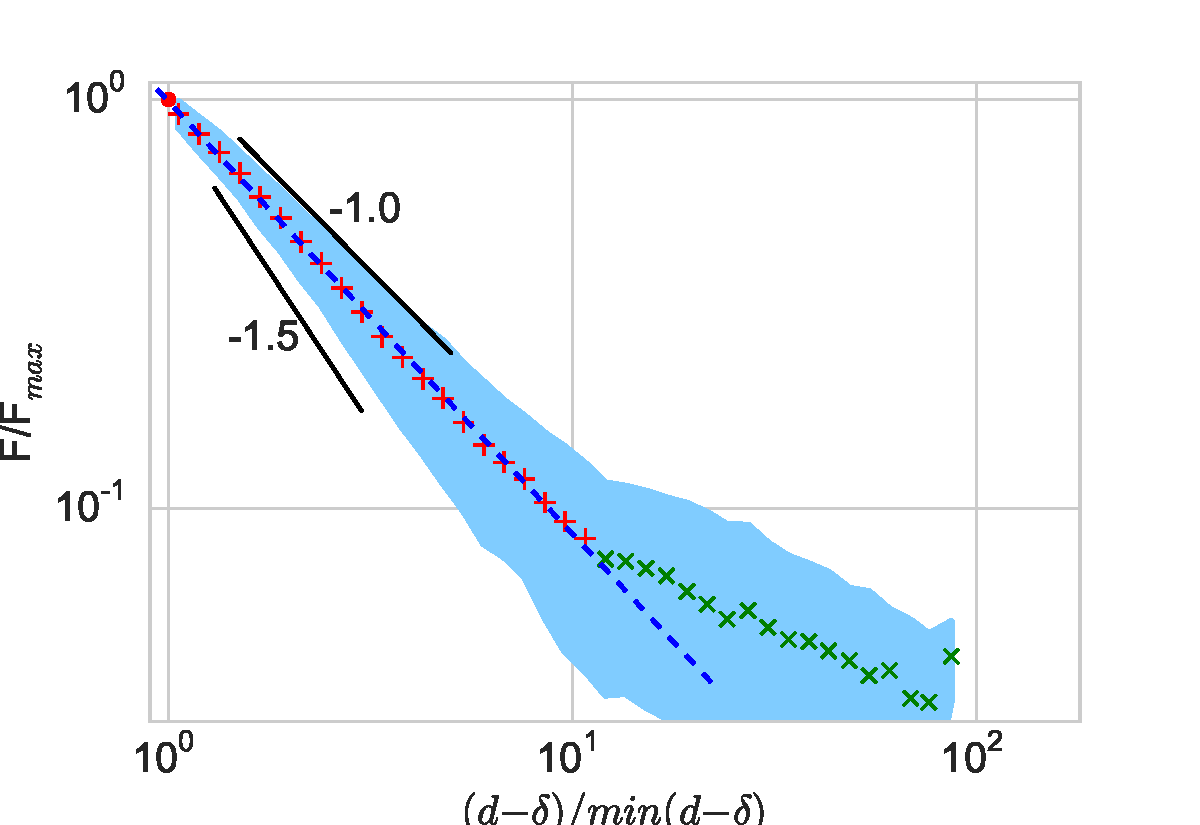
\includegraphics[width=0.700\linewidth]{rescaled_powerlaw.pdf}
\caption{Representation of rescale approach data on a log-log scale.  Red and green
crosses correspond to average values. Blue area corresponds to average +/-
standard deviation for each average bin. Red dot in the upper right corner
corresponds to the point (1,1) with respect to which all data have been
rescaled.}{\small 
Blue dashed line shows a power law fit of the average data for
\(d_c/d_{c,min} < 10\) (red cross), fitted slope is \(-1.06\) .
As an eye guide, the slopes of \emph{-1} and \emph{-1.5} have been represented.
}\label{index-latex:fig-rescale-powerlaw}\end{figure}

The rescaled data confirm an average power law exponent of \(\sim -1\), the
breakdown of the average exponent beyond \(d_c/d_{c,min}=10\) can be
explained by the statistical effect due to a lack of data for long distance.


\subsection{Variation of parameters with Capping Protein}
\label{index-latex:variation-of-parameters-with-capping-protein}
At the chosen concentration of Arp2/3, the bead system can show symmetry
breaking in the correct range of a Capping Protein concentration of 10 to 30
µM. In absence of Capping Protein, the dense dendritic network does not form on
the surface {\hyperref[index-latex:kawska2012]{{[}Kawska et al. 12{]}}}. At low Capping Protein concentrations (\(<10 \mu{}M\)) it seems not able to generate enough stress to
rupture, and at too high concentrations (\textgreater{}35nM, the visible gel is thin and does
not break symmetry either. We then investigated the variation of each fit parameters for Capping Protein concentrating ranging from 0 to 50 nM.

We have already,  seen  that the power law exponent factor \(\alpha\)
didn't vary with the amount of Capping Protein in solution (\hyperref[index-latex:power-law-exponent]{Figure  \ref*{index-latex:power-law-exponent}}).
The two other investigated parameters are the prefactor
\(\beta\) and distance offset \(\delta\) . For the same value of \(\alpha\) and \(\delta\), the
higher \(\beta\) is, the stronger the interaction between the two beads for
the same distance \(d_c\). We can see on \hyperref[index-latex:beta-violin]{figure  \ref*{index-latex:beta-violin}} that the
average value for the prefactor decreases in accordance with the increasing of Capping Protein
concentration.
\begin{figure}[htbp]
\centering
\capstart

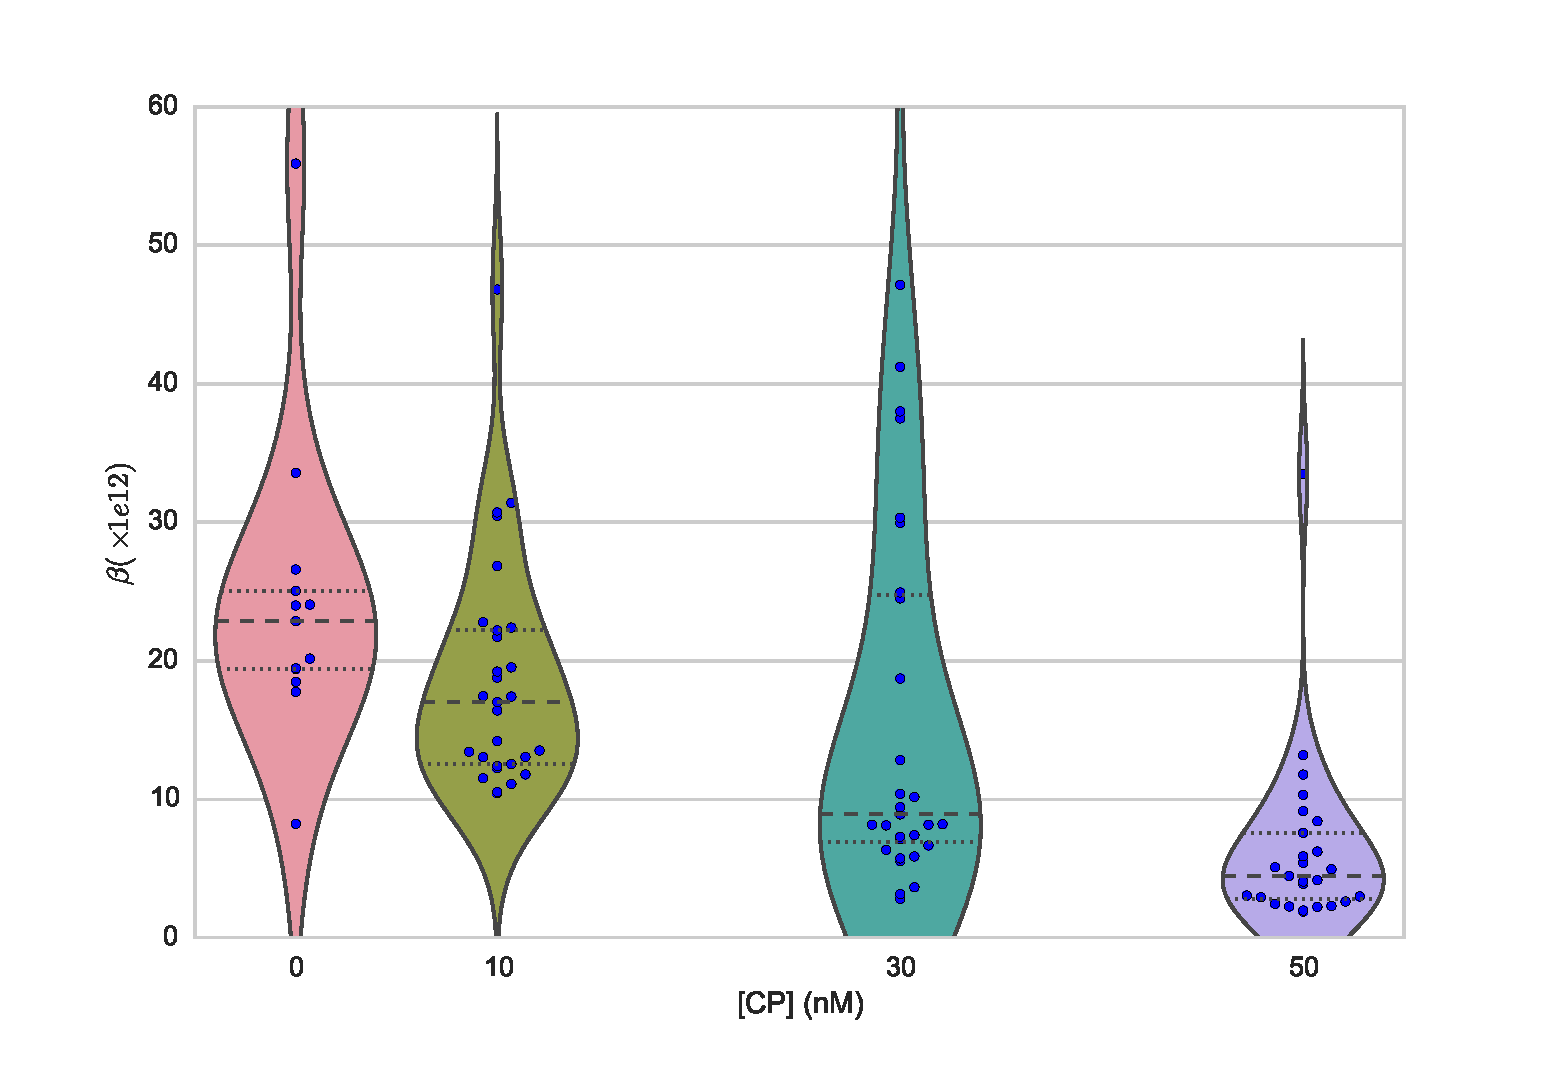
\includegraphics[width=0.800\linewidth]{beta_violin.pdf}
\caption{Violin plot showing the repartition of the prefactor with the quantity of
Capping Protein. The decrease of prefactor with an increasing amount of Capping
Protein indicates a lower force between the probe-bead and the actin bead,
for the same corrected distance between bead centers.}\label{index-latex:beta-violin}\end{figure}

The last parameter of our model is \(\delta\), the distance at which the force
diverges.   It can be seen in \hyperref[index-latex:delta-violin]{figure  \ref*{index-latex:delta-violin}} that with the exception
of zero Capping Protein, the distance at which the model diverges gets
closer to the polystyrene bead diameter, as the concentration of Capping
Proteins in the medium increases. It is interesting to note that the distance offset
\(\delta\) is very close from the bead diameter in the absence of Capping Protein, when no
biomimetic actin cortices forms.
\begin{figure}[htbp]
\centering
\capstart

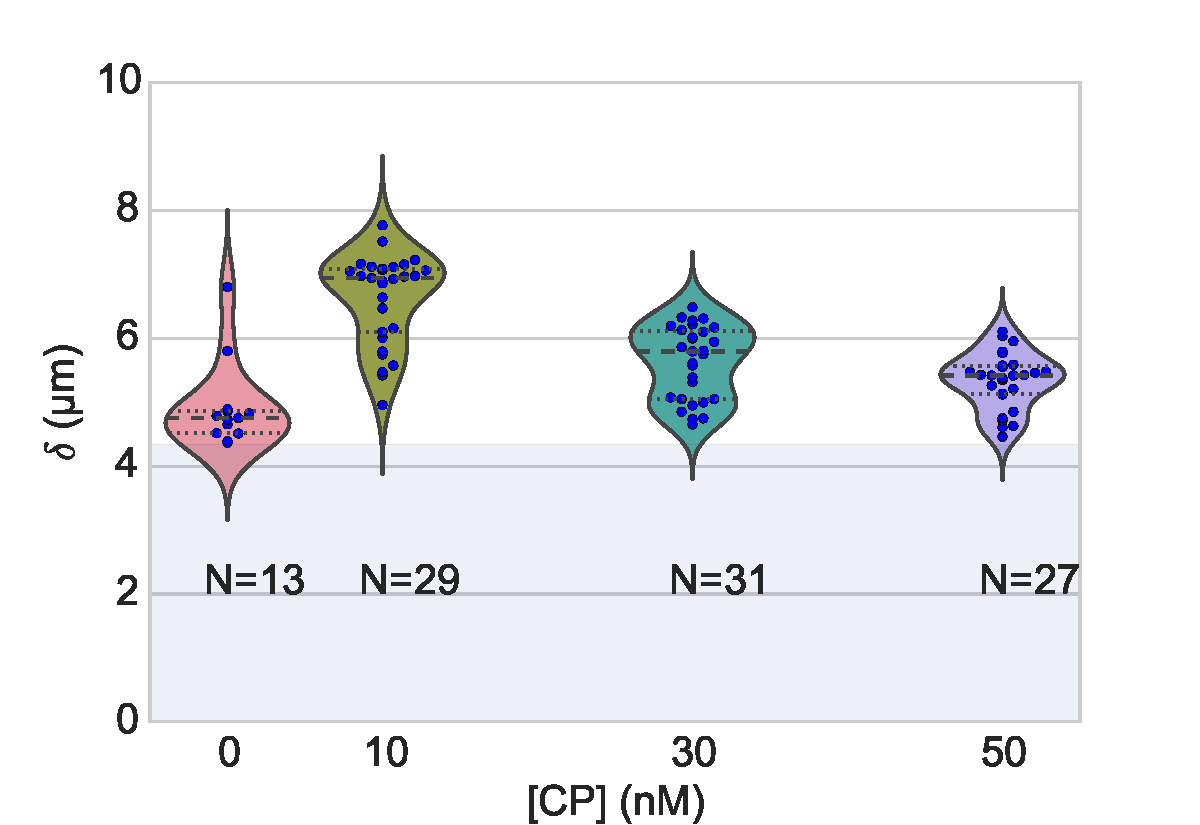
\includegraphics[width=0.800\linewidth]{delta_violin.pdf}
\caption{Violin plot showing the variation of the offset distance \(\delta\)
with the Capping Protein concentration. The shaded area represents the
non-physical region which would correspond to a diverging force beyond the
contact of the two polystyrene beads. Experimental data with \(\delta\)
value in this region have been excluded from further analysis.}\label{index-latex:delta-violin}\end{figure}


\subsection{Determination of Young's Modulus}
\label{index-latex:determination-of-young-s-modulus}
In order to determine the gel mechanical properties between the actin and the
probe bead, we modelled it as a purely elastic material. The viscous effects are
neglected in the approach part, as the approach at different speeds shows no
clear effect on the approach curves (\hyperref[index-latex:many-speed]{Figure  \ref*{index-latex:many-speed}}). We considered
the compression of the material between the two beads. The surface of the
compressed material is approximated by the bead projected surfaces of the bead along the
direction of compression (\(\pi R^2\)).  The thickness of the compressed
material is regarded as the distance between bead centers corrected by the
distance offset \(\delta\), as any material below delta can be considered as
infinitively rigid for the optical tweezer.

The stress exerted onto the material projected onto the bead surface or radius
\(R\) can be written :
\phantomsection\label{index-latex:equation-eqa32}\begin{gather}
\begin{split}\sigma = \frac{F}{\pi R^2}\end{split}\label{index-latex-eqa32}
\end{gather}
For a minor deformation, the local strain of the material \(u\) can be written
as a function of the corrected bead position \(d_c\) and the considered location
along the axis between the two bead center as \(x\) :
\phantomsection\label{index-latex:equation-eqa33}\begin{gather}
\begin{split}u(x)= \frac{d_c-x}{d_c}\end{split}\label{index-latex-eqa33}
\end{gather}
We can express the local differential strain around the bead position \(d_c\) : \(\partial u = -\partial x/ \partial d_c\) in which the minus sign
reflects the choice of the coordinate system: a decrease in \(x\) with a
positive Young's modulus \(E\) should lead to an increase of the exerted force.
The locally felt Young's modulus
at the distance \(d_c\) is then
\phantomsection\label{index-latex:eq-e}\phantomsection\label{index-latex:equation-eqa34}\begin{gather}
\begin{split}E(d_c) = \left.\frac{\partial\sigma}{\partial u}\right|_{d_c}\end{split}\label{index-latex-eqa34}
\end{gather}
By injecting the expression of \(u\) and \(\sigma\) this lead to :
\phantomsection\label{index-latex:equation-eqa35}\begin{gather}
\begin{split}E(d_c) &= -\frac{d_c}{\pi R^2}\times \Big(\frac{dF}{dx}\Big) \Big|_{x=d_c}\\
     &= E_0 d_c^\alpha\end{split}\label{index-latex-eqa35}
\end{gather}
in which the value of \(E_0\) can be expressed as function of the power law exponent \(\alpha\) and the prefactor \(\beta\) :
\phantomsection\label{index-latex:equation-eqa36}\begin{gather}
\begin{split}E_0 = - \frac{\alpha\beta}{\pi R^2}\end{split}\label{index-latex-eqa36}
\end{gather}
Experimentally, the probed Young's modulus corresponds to the average mechanical
properties of the actin cloud between the actin bead surface and the
probe-bead surface and does not reflect the variation of the uncompressed actin cloud mechanical
properties with position.
Physically \(E_0\) corresponds to the Young's modulus as a corrected distance of \(d_c = 1 \mu{}m\)
(See \hyperref[index-latex:ev]{Figure  \ref*{index-latex:ev}})
The geometry of the
system and the fluorescence signal suggest a decrease of the actin cloud density according to the distance from the actin-bead center. All values
reported later represent an estimation of the effective Young’s modulus elasticity. The value of this effective Young's modulus is 3 orders of magnitude
smaller than the acknowledged elasticity of dendritic gels formed on beads, measured in the
order of kPa {\hyperref[index-latex:marcy2004]{{[}Marcy et al. 04{]}}}.

This difference in elasticity might explain why the mechanical actions of this actin cloud have not been
confirmed before in other measurements, like micro-pipette aspiration,
micro needle deformation or Atomic Force Microscopy indentation that have
sensitivities in the order of nN, while the forces exerted by this actin cloud
are in the order of pN.

Nonetheless, {\hyperref[index-latex:gardel2003]{{[}Gardel et al. 03{]}}} shows that such low moduli can be obtained using
sparse entangled actin networks, and confirms the idea that the actin-cloud seen
with the optical-tweezer indent experiments, has a fundamentally different
structure than the dense dendritic network on the actin
bead surface.
\begin{figure}[htbp]
\centering
\capstart

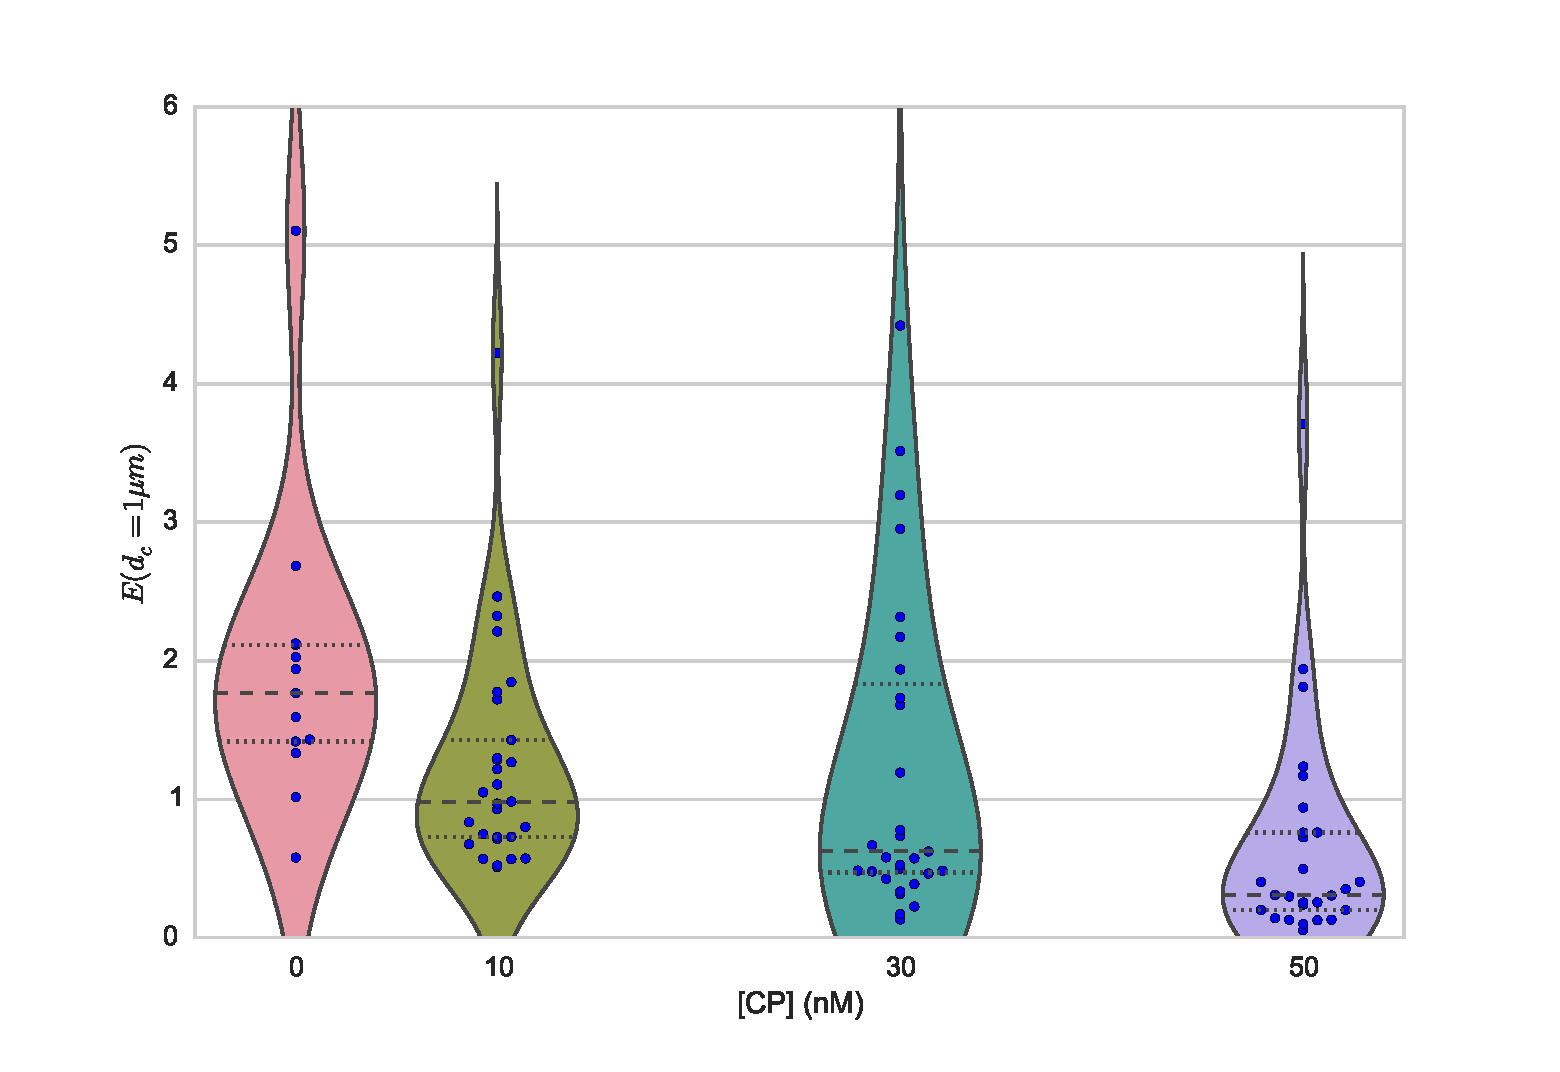
\includegraphics[width=0.800\linewidth]{E0_violin.pdf}
\caption{Young's Modulus prefactor, as a function of Capping Protein, shows a decrease of the
average Young's modulus with an increase of Capping Protein concentration.}\label{index-latex:ev}\end{figure}


\subsection{Mechanical properties}
\label{index-latex:mechanical-properties}
To investigate the mechanical properties of the network that should arise from
a \(\alpha = -1\) power law, we modelled the actin cloud deformation by
the theory of semi-flexible entangled polymer networks ({\hyperref[index-latex:isambert1996]{{[}Isambert et al. 96{]}}},
{\hyperref[index-latex:mackintosh1995]{{[}MacKintosh et al. 95{]}}}, {\hyperref[index-latex:morse1998a]{{[}Morse 98a{]}}}).

The Young's modulus of semi-flexible filaments in a 3D environment can be
expressed as a function of the filament contour length density \(\rho\) and the
entanglement length \(L_e\) as {\hyperref[index-latex:morse1998b]{{[}Morse 98b{]}}}:
\phantomsection\label{index-latex:equation-eqa37}\begin{gather}
\begin{split}E= \frac{2.(1+\nu).7.k_BT \rho}{5L_e}\end{split}\label{index-latex-eqa37}
\end{gather}
In which \(\nu\) is the Poisson’s ratio that allows the conversion from shear to
elastic modulus. Previous studies have investigated the non-linear stiffening of
such actin networks for large deformation {\hyperref[index-latex:semmrich2008]{{[}Semmrich et al. 08{]}}} and found that in
our condition, the linear description of these networks holds to describe the
actin cloud.

As {\hyperref[index-latex:morse1998a]{{[}Morse 98a{]}}} we expressed the entanglement length as a
function of persistence length and filament density: \(L_e\approx L_p^{1/5} \rho^{-2/5}\). We can
reduce the expression of the Young's modulus to a function of the following
parameters :
\begin{itemize}
\item {} 
The Poisson’s Ratio \(\nu\),

\item {} 
The persistence length of actin filaments \(L_p\)

\item {} 
The mesh size of the network \(\xi_0^2 = \rho_0\)

\item {} 
The ``size'' of the cloud, for which we use the distance where the force
is first significant \(d_0\)

\end{itemize}

We also need to consider that for a general compressible material, the
only variable that changes during compression is the density \(\rho\)
which can be expressed as a function of the corrected distance \(\rho \to
\rho(d_c)\)

Thus leading to :
\phantomsection\label{index-latex:equation-eqa}\begin{gather}
\begin{split}E(d_c)=\frac{ (1+\nu).14.k_BT}{5L_p^{1/5}}\times \rho(d_c)^{7/5}\end{split}\label{index-latex-eqa}
\end{gather}
The scaling exponent of \(E\) in equation \eqref{index-latex-eqa} with \(d_c\) should match the exponent
of the experimentally found power law \(\alpha\). Thus, the density can be
expressed in the following form :
\phantomsection\label{index-latex:equation-eq-rho}\begin{gather}
\begin{split}\rho(d_c)=\rho_0(d_c/d_0)^{5/7\times\alpha}\end{split}\label{index-latex-eq-rho}
\end{gather}
By defining \(\rho\) in {\hyperref[index-latex:morse1998a]{{[}Morse 98a{]}}}, which is
the filament contour length per unit volume, we can determine the
mesh-size \(\xi_0\) of the undeformed network:
\phantomsection\label{index-latex:equation-eqa38}\begin{gather}
\begin{split}\xi_0 = 1/\sqrt\rho_0\end{split}\label{index-latex-eqa38}
\end{gather}
By comparing this to the phenomenological fit, we can express the elastic
modulus as a function of the distance, and the mesh size, as a function of the
fit parameters and the characteristic scales of the system.
\phantomsection\label{index-latex:equation-eqb}\begin{gather}
\begin{split}E(d_c)     &=  \frac{(1+\nu).14.k_BT}{5L_p^{1/5}\xi_0^{14/5} \left.d_0\right.^{\alpha}}\times \left.d_c\right.^{\alpha}.\\
                &=  E_0' \times \left.d_c\right.^{\alpha}\end{split}\label{index-latex-eqb}
\end{gather}
In which \(E_0'\) can be identified as \(E_0\) in \eqref{index-latex-eqa} to extract the
closed form solution for the mesh size \(\xi_0\) :
\phantomsection\label{index-latex:equation-eqa39}\begin{gather}
\begin{split}\xi_0=\left(-\frac{({2-\frac{5}{7}\alpha)}.k_BT\pi R^2}{5\alpha \beta L_p^{\frac{1}{5}}\left.d_0\right.^{\alpha}}\right)^{\frac{5}{14}}\end{split}\label{index-latex-eqa39}
\end{gather}
The found mesh size is in the order of 0.3 to 0.4 µm, which is consistent with previous findings
:\emph{Morse1998b}. The variation of the
mesh size can be seen on \hyperref[index-latex:xi-violin]{figure  \ref*{index-latex:xi-violin}} and does not seem to have a
correlation with the Capping Protein concentration.
\begin{figure}[htbp]
\centering
\capstart

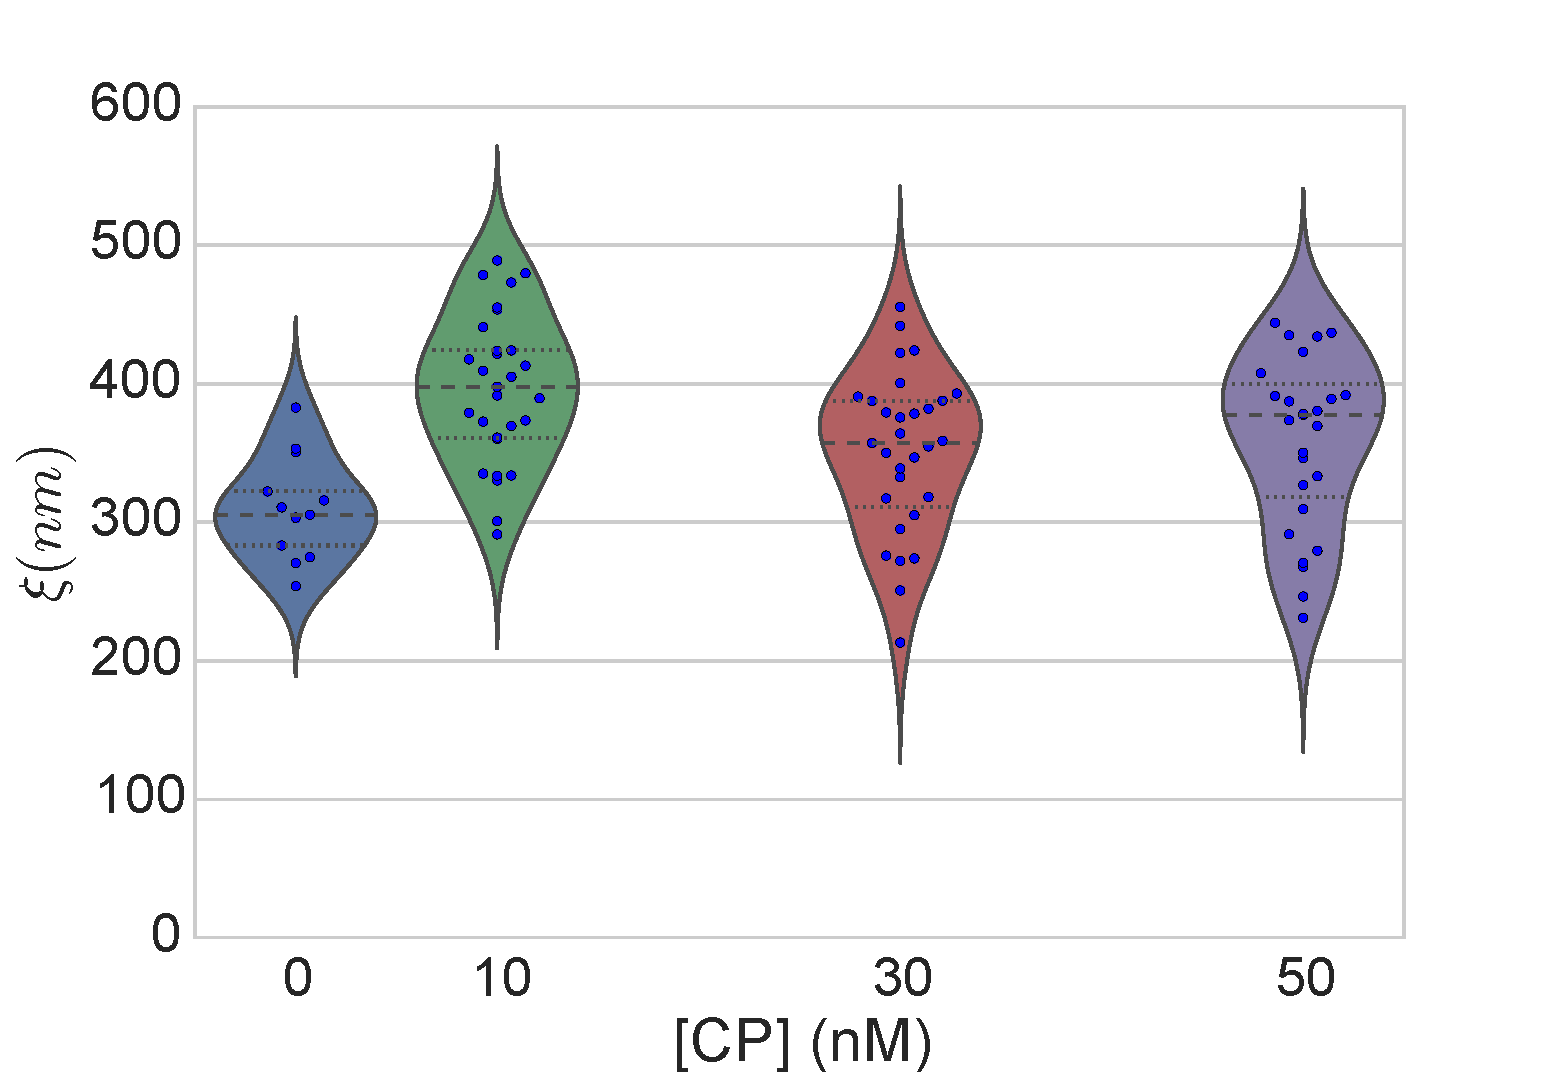
\includegraphics[width=0.800\linewidth]{xi_violin.pdf}
\caption{Meshsize vs Capping plot.}\label{index-latex:xi-violin}\end{figure}

We explored the correlation between the mesh size and \(\delta\) by plotting  the mesh size against the distance offset \(\delta\) (\hyperref[index-latex:dxcf]{Figure  \ref*{index-latex:dxcf}}).
\hyperref[index-latex:dxf]{Figure  \ref*{index-latex:dxf}} shows the relation between the mesh size and the offset
distance \(\delta\) regardless of each Capping Protein concentration.
\begin{figure}[htbp]
\centering
\capstart

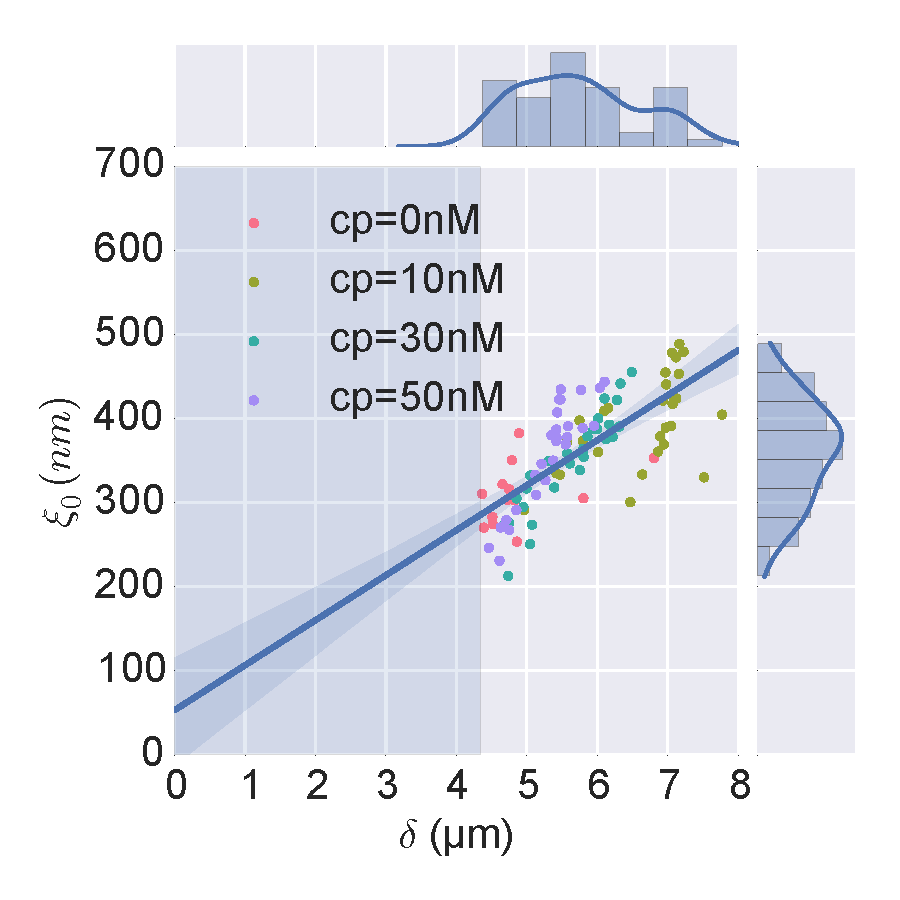
\includegraphics[width=1.000\linewidth]{delta-xi-corr.pdf}
\caption{Correlation of the meshsize \(\xi_0\) with the distance offset \(\delta\),
with marginal distribution as per histogram on the side and on the top.  Shaded
regions represent confidence interval at 95\%.}\label{index-latex:dxcf}\end{figure}
\begin{figure}[htbp]
\centering
\capstart

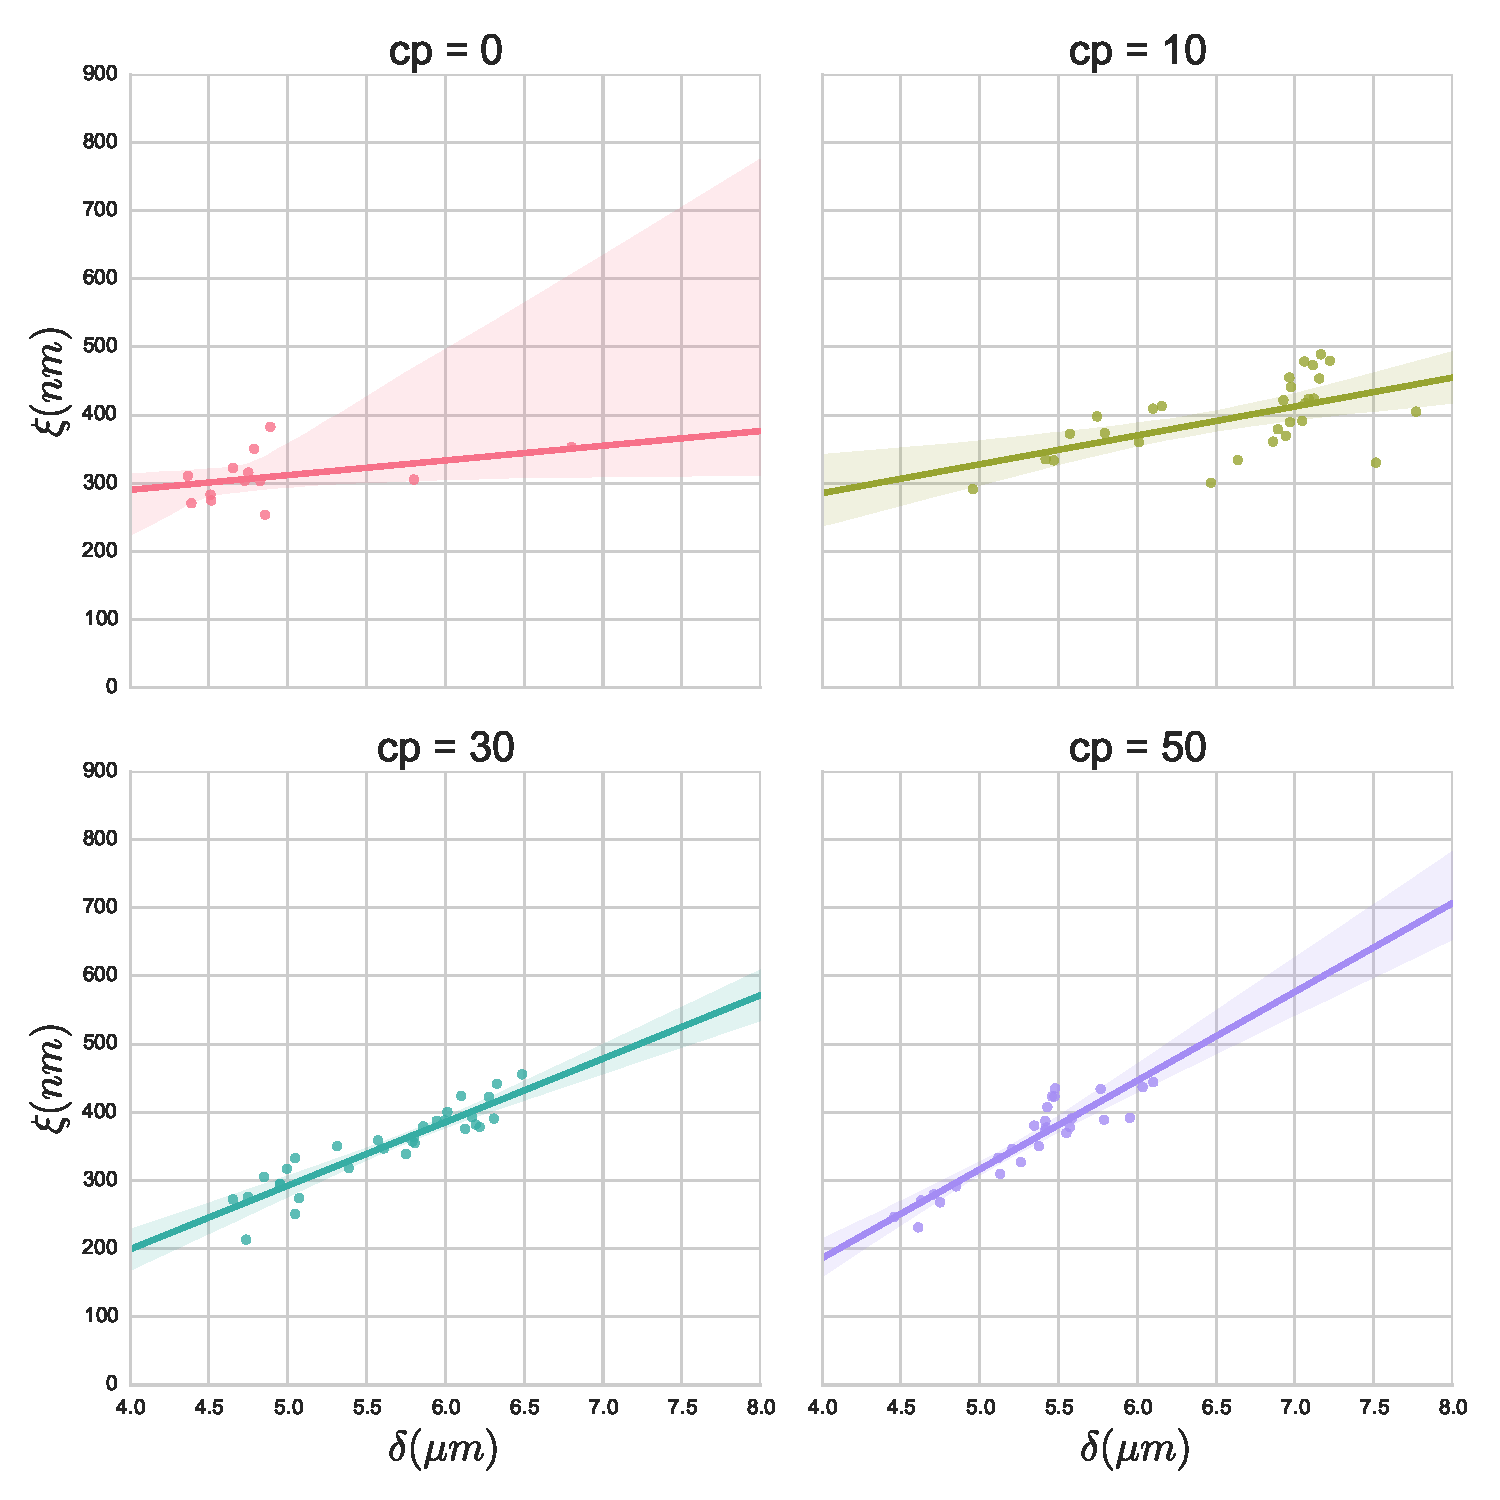
\includegraphics[width=1.000\linewidth]{delta-xi-facets.pdf}
\caption{Same figure as \hyperref[index-latex:dxcf]{ \ref*{index-latex:dxcf}} for each concentration of Capping Protein,
with linear regression and confidence intervals at 95\%.}\label{index-latex:dxf}\end{figure}

From \eqref{index-latex-eqa} and \eqref{index-latex-eqb} by identifying the prefactor, it is also possible
to extract the Poisson’s ratio (\(\nu\)) of the compressed material :
\phantomsection\label{index-latex:equation-nu=f(alpha)}\begin{gather}
\begin{split}\nu =\frac 1 2 \times \left( \frac 5 7.\alpha +1\right)\end{split}\label{index-latex-nu=f(alpha)}
\end{gather}
The Poisson’s ratio only depends on the power law exponent and thus slightly varies
with the amount of Capping Protein concentration.  We found a Poisson’s ratio value between 0.1 and 0.2, corresponding to compressible
foam-like materials that do not highly expand in the direction orthogonal to
the compression axis. A previous study of bulk actin network finds a Poisson’s
ration of 0.5 (incompressible material) for an actin concentration of 21.5 µM.  We
suspected that the low actin concentration used in our experiments (4µM) is the
reason for the low Poisson’s Ratio. The local structure of filaments
emanating from the  bead may also explain the large compressibility of our actin
cloud.


\subsection{Interpretation}
\label{index-latex:interpretation}
The results of our data analysis lead to the interpretation that
a dense actin gel with an elasticity close to \textasciitilde{}1kPa is polymerised
on the actin bead surface. This stiff gel
cannot be indented by the optical tweezer. Beyond this dense gel, a soft
actin cloud with an effective elastic modulus of 1 Pa and below is
present and extends on distances several times bigger than the thickness
of the reconstituted actin cortex (\hyperref[index-latex:fig-interpretation]{Figure  \ref*{index-latex:fig-interpretation}}). The
structure of this actin cloud is expected to be quite different from the
dendritic gel and to be mostly constituted of loosely entangled actin filaments.

In this model, the offset distance \(\delta\) corresponds to the limit of the dense
dendritic actin network mimicking the actin cortex that grows on actin beads.
The high elastic modulus of this gel makes it impenetrable for the small forces generated by the optical tweezer we use. The
values of \(\delta\) we found are coherent with the measured thickness \(e
\simeq \delta - 2.R_{bead}\) of the  biomimetic actin cortex, as measured by
epifluorescence in {\hyperref[index-latex:kawska2012]{{[}Kawska et al. 12{]}}} and found to be in the range of 1 to 2 µm. The decrease
of \(\delta\) with Capping Protein is also coherent with the decrease of gel
thickness.

The filaments composing the actin cloud directly emanate from the actin
cortex in which the actin polymerisation nucleation started at the bead surface
. Eventually, a few filaments can escape from the network and are
capped by the Capping Protein provided that the growing extremity is already several
micrometers from the bead surface.
\begin{figure}[htbp]
\centering
\capstart

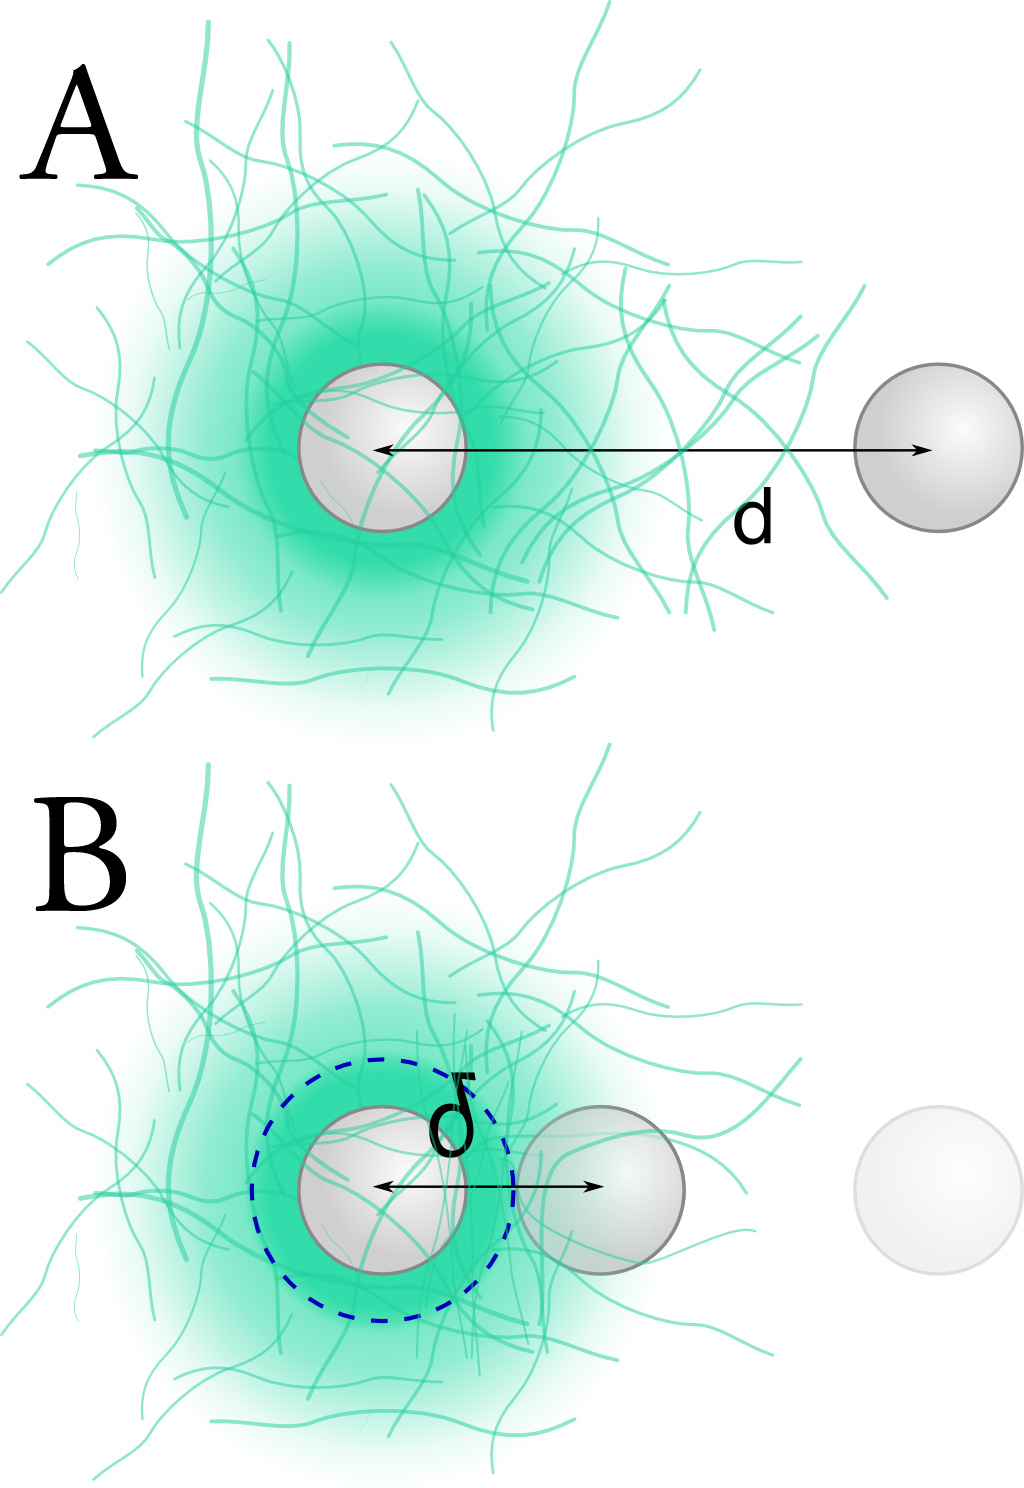
\includegraphics[width=0.900\linewidth]{interp-delta.png}
\caption{A ) Schematic of an actin cloud. Left:  The actin bead triggers actin
polymerisation. Right Probe Bead. On the actin bead surface, a dense
and dendritic network forms a biomimetic actin cortex with an elastic
modulus close to the kPa (Dark Green). From this actin cortex emanates a
softer actin structure : the actin cloud . The actin cloud is a loosely
entangled network formed by the filaments escaping from the bead's actin
cortex and extending over several micrometers. The actin cloud has an average
elastic modulus which is several orders of magnitude softer than the actin
cortex. B ) From the probe-bead point of view in the optical tweezer, the
system (actin-bead+actin cortex) behaves as a hard-sphere of radius
\(\delta-R\)}\label{index-latex:fig-interpretation}\end{figure}

The actin cortex thickness, \(e\) as measured in {\hyperref[index-latex:kawska2012]{{[}Kawska et al. 12{]}}},
increases with time during the actin polymerisation. We can predict that the
offset distance \(\delta\) should increase with time, except in the absence of
Capping Protein where no actin cortices form. This can be verified on
\hyperref[index-latex:time-delta-corr]{figure  \ref*{index-latex:time-delta-corr}} that shows the evolution of \(\delta\) as a function
of polymerisation time.
\begin{figure}[htbp]
\centering
\capstart

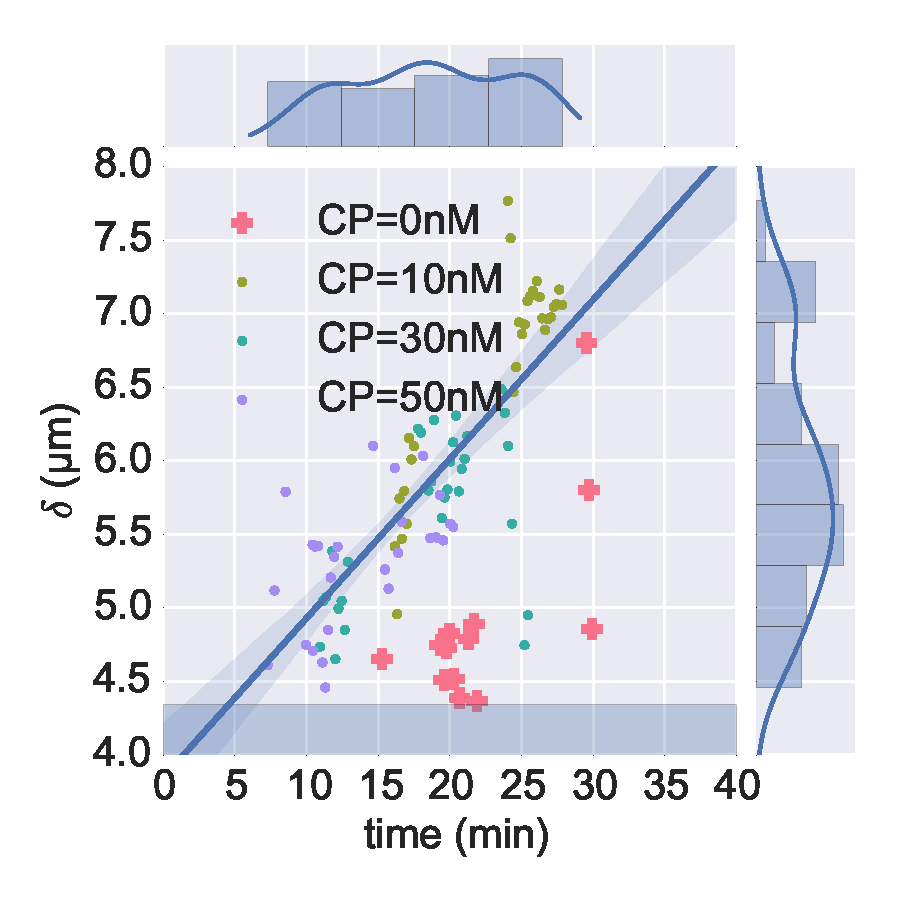
\includegraphics[width=0.900\linewidth]{time-delta-corr.pdf}
\caption{Distance offset \(\delta\) as a function of time (min) since mix of actin, ATP
and beads. Linear fit with confidence interval at 95\% (light shaded area)
and bead surface (dark shaded area). Samples taken in the absence of Capping
Protein are not taken into account in the regression (Pink +). The increase
of \(\delta\) with time is coherent with the measured increase of the gel
thickness \(e\) as measured in {\hyperref[index-latex:kawska2012]{{[}Kawska et al. 12{]}}}}\label{index-latex:time-delta-corr}\end{figure}


\section{Relaxation phase}
\label{index-latex:id29}
The approach phase of the indentation cycle has been modelled with a purely
elastic mode. However, the force-distance plot shows a significant dissipation
marked by an hysteresis \hyperref[index-latex:force-distance]{Figure  \ref*{index-latex:force-distance}}. The repetitive indent cycle, giving the same
force-distance curves (\hyperref[index-latex:reproc]{Figure  \ref*{index-latex:reproc}}), allows to exclude a plastic deformation.
We can hence reject the hypothesis of ruptures of the
actin meshwork or breakage near the entanglement points.

The entangled filaments networks theory that allowed us to understand the link between the phenomenological
model and the mechanical properties of the network, also proposes a relation to
explain the network relaxation.

In this model {\hyperref[index-latex:morse1998a]{{[}Morse 98a{]}}}, the visco elastic modulus  \(E\) is a function of time
and can be written as \(E(t) = E\times \chi(t)\) with
\phantomsection\label{index-latex:equation-chi}\begin{gather}
\begin{split}\chi(t)=\sum_{n, odd} \frac{8}{n^2 \pi^2}exp\left(- \frac{n^2\pi^2 t}{ \tau_{rep}} \right)\end{split}\label{index-latex-chi}
\end{gather}
In which \(\tau_{rep} = \frac{l_f^2}{D_{rep}}\) is a single fit parameter
depending on diffusion constant for filament reptation \(D_{rep}\) and the
filaments length \(l_f\). In this form, \(\chi\) is a sum of
exponential decays with well defined characteristic timescales and amplitudes
that decrease as \(1/n^2\). To fit this model to the
relaxation phase data, we can limit ourselves to the first 40 terms of the sum, as
any of the subsequent terms represent timescales, we cannot reach with our
experimental resolution.

It should be noted that the value of \(\chi(t=0)\) is 1 and should be
treated particularly in order to ensure continuity of the force applied on the
actin-bead in the model.

Using this sum of exponential decays is coherent with the common conclusions of
power-laws found in the frequency-dependant shear modulus of both \emph{in vivo} and \emph{in vitro} actin
networks, as well as the relaxation behaviour found in cells.

In order to determine \(\tau_{rep}\), the Young's modulus established  in the
approach phase is used and the model is fitted against the relaxation data.  A
result of such a fit can be observed on \hyperref[index-latex:fit-3-phases]{figure  \ref*{index-latex:fit-3-phases}}. The values of
\(\tau_{rep}\) are highly variable and the fit can be difficult when the relaxation is
slow or in the order of the measured noise. The variation of \(\tau_{rep}\) with the
concentration in Capping Protein can be seen on \hyperref[index-latex:tau-violin]{figure  \ref*{index-latex:tau-violin}}, and
one example of fit on the \hyperref[index-latex:fit-3-phases]{figure  \ref*{index-latex:fit-3-phases}}
\begin{figure}[htbp]
\centering
\capstart

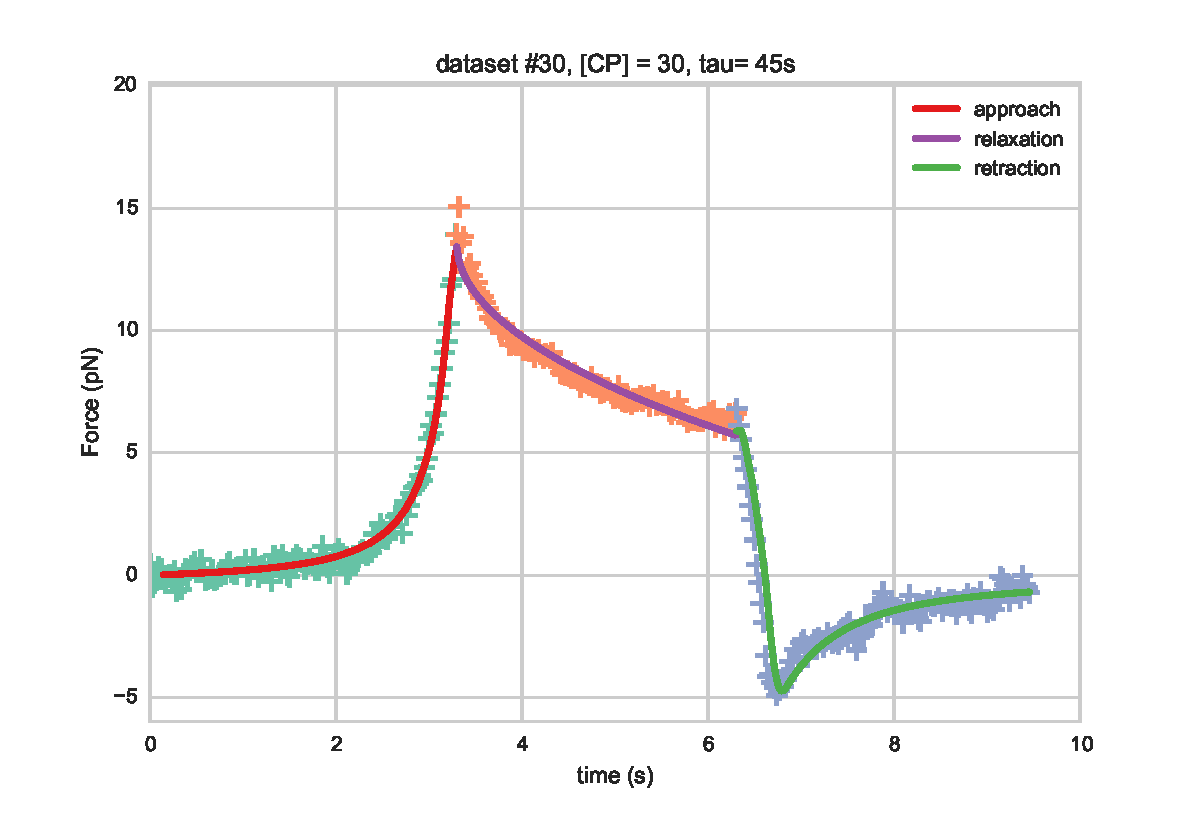
\includegraphics[width=0.800\linewidth]{3phases.pdf}
\caption{Force as a function of time as well as fit for the 3 phases, approach,
relaxation and retraction.}\label{index-latex:fit-3-phases}\end{figure}
\begin{figure}[htbp]
\centering
\capstart

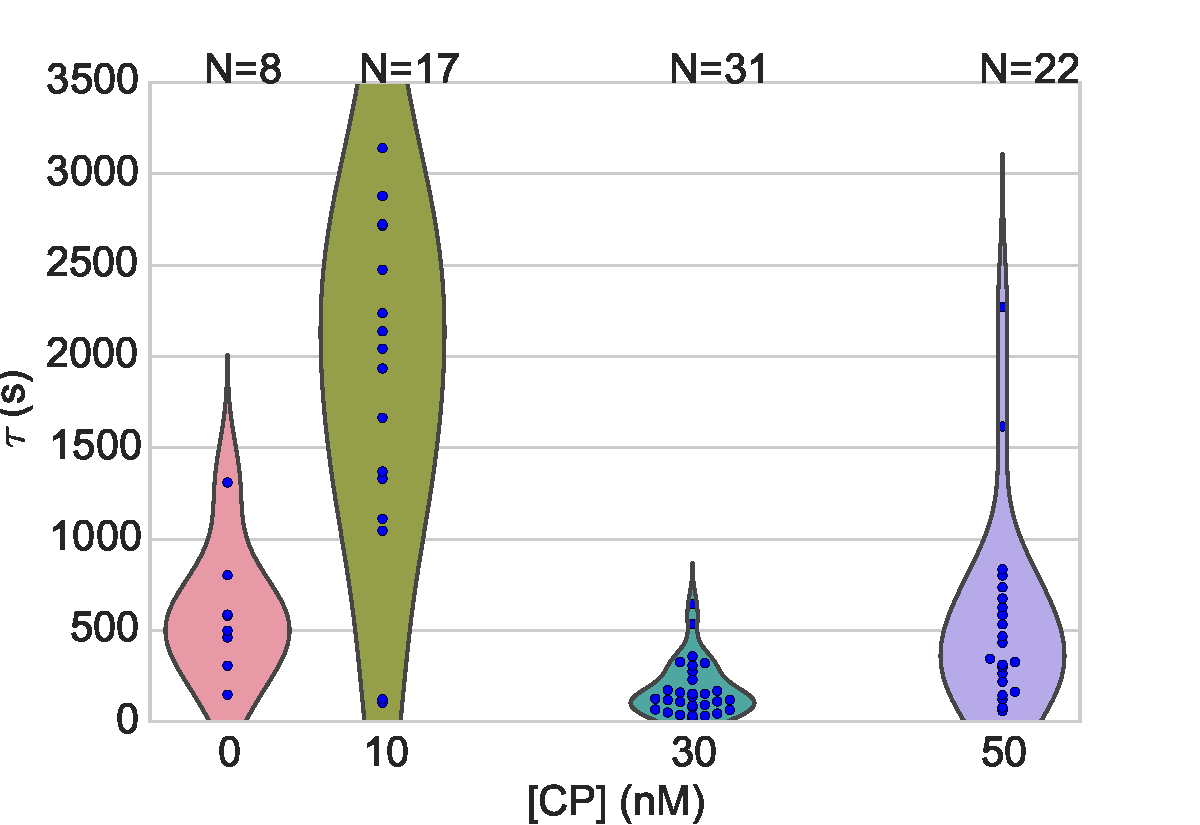
\includegraphics[width=0.800\linewidth]{tau_violin.pdf}
\caption{Violin plot showing the repartition of \(\tau_{rep}\) as a function of capping
protein. Outlier (\(\tau_{rep}\) negative or greater than tens of minutes removed)}\label{index-latex:tau-violin}\end{figure}

We can see here that the polymer model introduced in {\hyperref[index-latex:morse1998a]{{[}Morse 98a{]}}} allows
to completely fit the succession of approach and relaxation phases.  In order to check whether
the fit parameters give realistic values, we can estimate the diffusion constant
for filament reptation \(D_{rep}\).
\phantomsection\label{index-latex:equation-eqa3-10}\begin{gather}
\begin{split}D_{rep} &= \frac{k_bT}{\gamma l_f} \\\end{split}\label{index-latex-eqa3-10}
\end{gather}
In which \(\gamma\approx {2\pi\eta_s}/{ln(\xi_0/d_f)}\) is the friction
coefficient per unit length. \(\gamma\) depends on the solvent viscosity
\(\eta_s\), the mesh-size \(\xi_0\) and the filament diameter
\(d_f\) (\(~7nm\) for actin).  We use \(\eta_s=10^{-3} Pa\times s\)
for water and a mesh size in the order of 400nm as determined from the approach phase
(\hyperref[index-latex:tau-violin]{Figure  \ref*{index-latex:tau-violin}}). Using \(\tau_{rep}\) given by the fit, this leads to filaments
length ranging from 3 to 8 µm, which is consistent with TIRF experiments and simulation as done in {\hyperref[index-latex:kawska2012]{{[}Kawska et al. 12{]}}}.


\subsection{Retraction Phase}
\label{index-latex:retraction-phase}
During the retraction phase the force decreases, becomes negative after a
retraction of 3 to 4 µm, and shows a slow  return to 0 at large distance.
Sticking events can be observed when the force becomes abruptly negative before
relaxing as fast. \hyperref[index-latex:sticking-event]{Figure  \ref*{index-latex:sticking-event}} shows such a sticking event
happening during an indentation cycle.
\begin{figure}[htbp]
\centering
\capstart

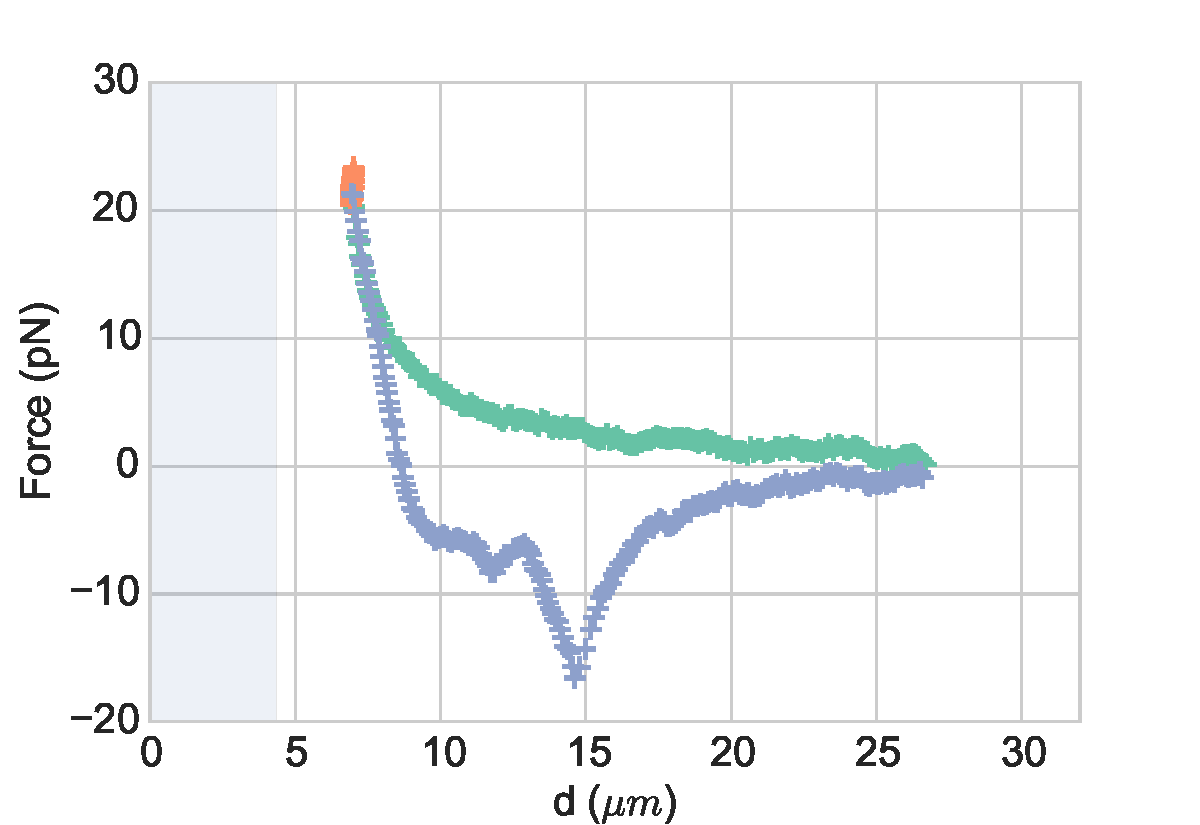
\includegraphics[width=0.800\linewidth]{sticking-event.pdf}
\caption{A sticking event at \(d=15\mu{}m\) where the rapidly decreasing force can be determined to go
up to -18 pN, before quickly returning to its normal value. A second smaller
sticking event is present at \(d=12\mu{}m\). Sticking events roughly appearing in 20\% of
the experiments.}\label{index-latex:sticking-event}\end{figure}

We assume that the sticking events are characteristic of non-specific interactions
between the probe-bead and the actin cloud. If no sticking event
is present, we assume the partial closing of the actin cloud beyond the
probe-bead during the relaxation phase, and model the retraction curve as a
transition between the damped-approach curve and a penetration of the probe-bead through the closing actin cloud.

During the approach phase, the force exerted on the actin-bead is
\(F(d)=\beta(d-\delta)^\alpha\). During the relaxation phase, the force
decreases from \(F(t_1)\) to \(F(t_2)\) with the relation :
\phantomsection\label{index-latex:equation-eqa311}\begin{gather}
\begin{split}\frac{F(t_2)}{F(t_1)} = \chi(t_2-t_1)\end{split}\label{index-latex-eqa311}
\end{gather}
We can write that the force exerted on the actin-bead during the retraction  can be expressed as a sum of the force felt during the approach, damped during the
relaxation (\(F_{da}\)), plus a force due to the closing of the actin
network behind the bead \(F_{closing}\).
\phantomsection\label{index-latex:equation-eqa312}\begin{gather}
\begin{split}F_{ret}(d) &= F_{da}(d) + F_{closing}(d)\\
F_{ret}(d) &= \chi(t_2-t_1).\beta(d-\delta)^\alpha+ F_{closing}(d)\end{split}\label{index-latex-eqa312}
\end{gather}
\(F_{closing}\) is computed using the fit parameter \(\alpha\), \(\beta\), \(\delta\) and \(\tau_{rep}\) (\hyperref[index-latex:retract-powerlaw]{Figure  \ref*{index-latex:retract-powerlaw}}).

On a double logarithmic scale and at long distance \(F_{closing}\) also seems to
follow a power law (\(F_{plaw}\)), when no sticking events are present.
\begin{figure}[htbp]
\centering
\capstart

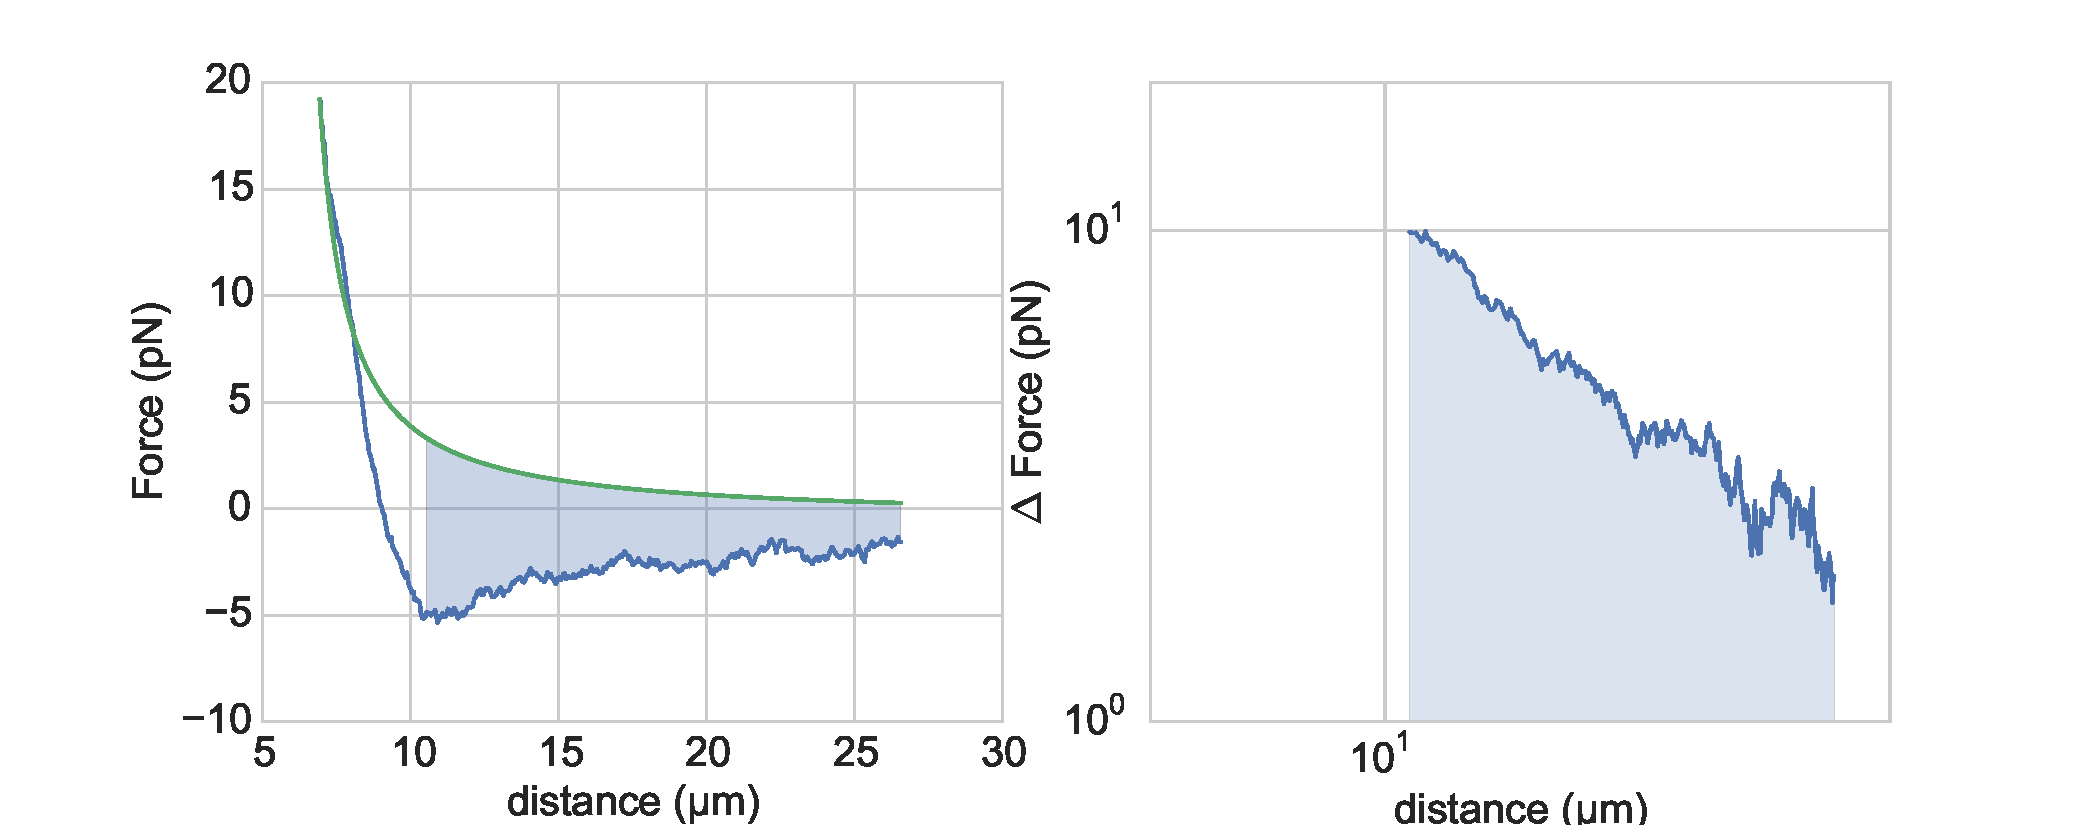
\includegraphics[width=1.000\linewidth]{retract-powerlaw.pdf}
\caption{Left : Retraction phase, with approach phase fit damped by
\(\chi(t_2-t1)\) in green. Blue area under the curve is plotted on a
log-log scale on the right, and follows a power law.}\label{index-latex:retract-powerlaw}\end{figure}

\(F_{ret}(d)\) though, seems to follow the force felt during the approach phase,
damped by \(\chi(t)\) (\(F_{da}\)) for \(d\simeq{D_{bead}}\) and
\(F_{da}+F_{plaw}\) for \(d > 10\mu{}m\).  The
typical bead size being \(D_{bead}\), we expect the transition from
one regime to the other to be done on a length scale of \(D_{bead}\). Thus
we use a smoothing function which is a convolution between the projected bead
area and a linear ramp function one can observe on \hyperref[index-latex:interp]{figure  \ref*{index-latex:interp}}
\begin{figure}[htbp]
\centering
\capstart

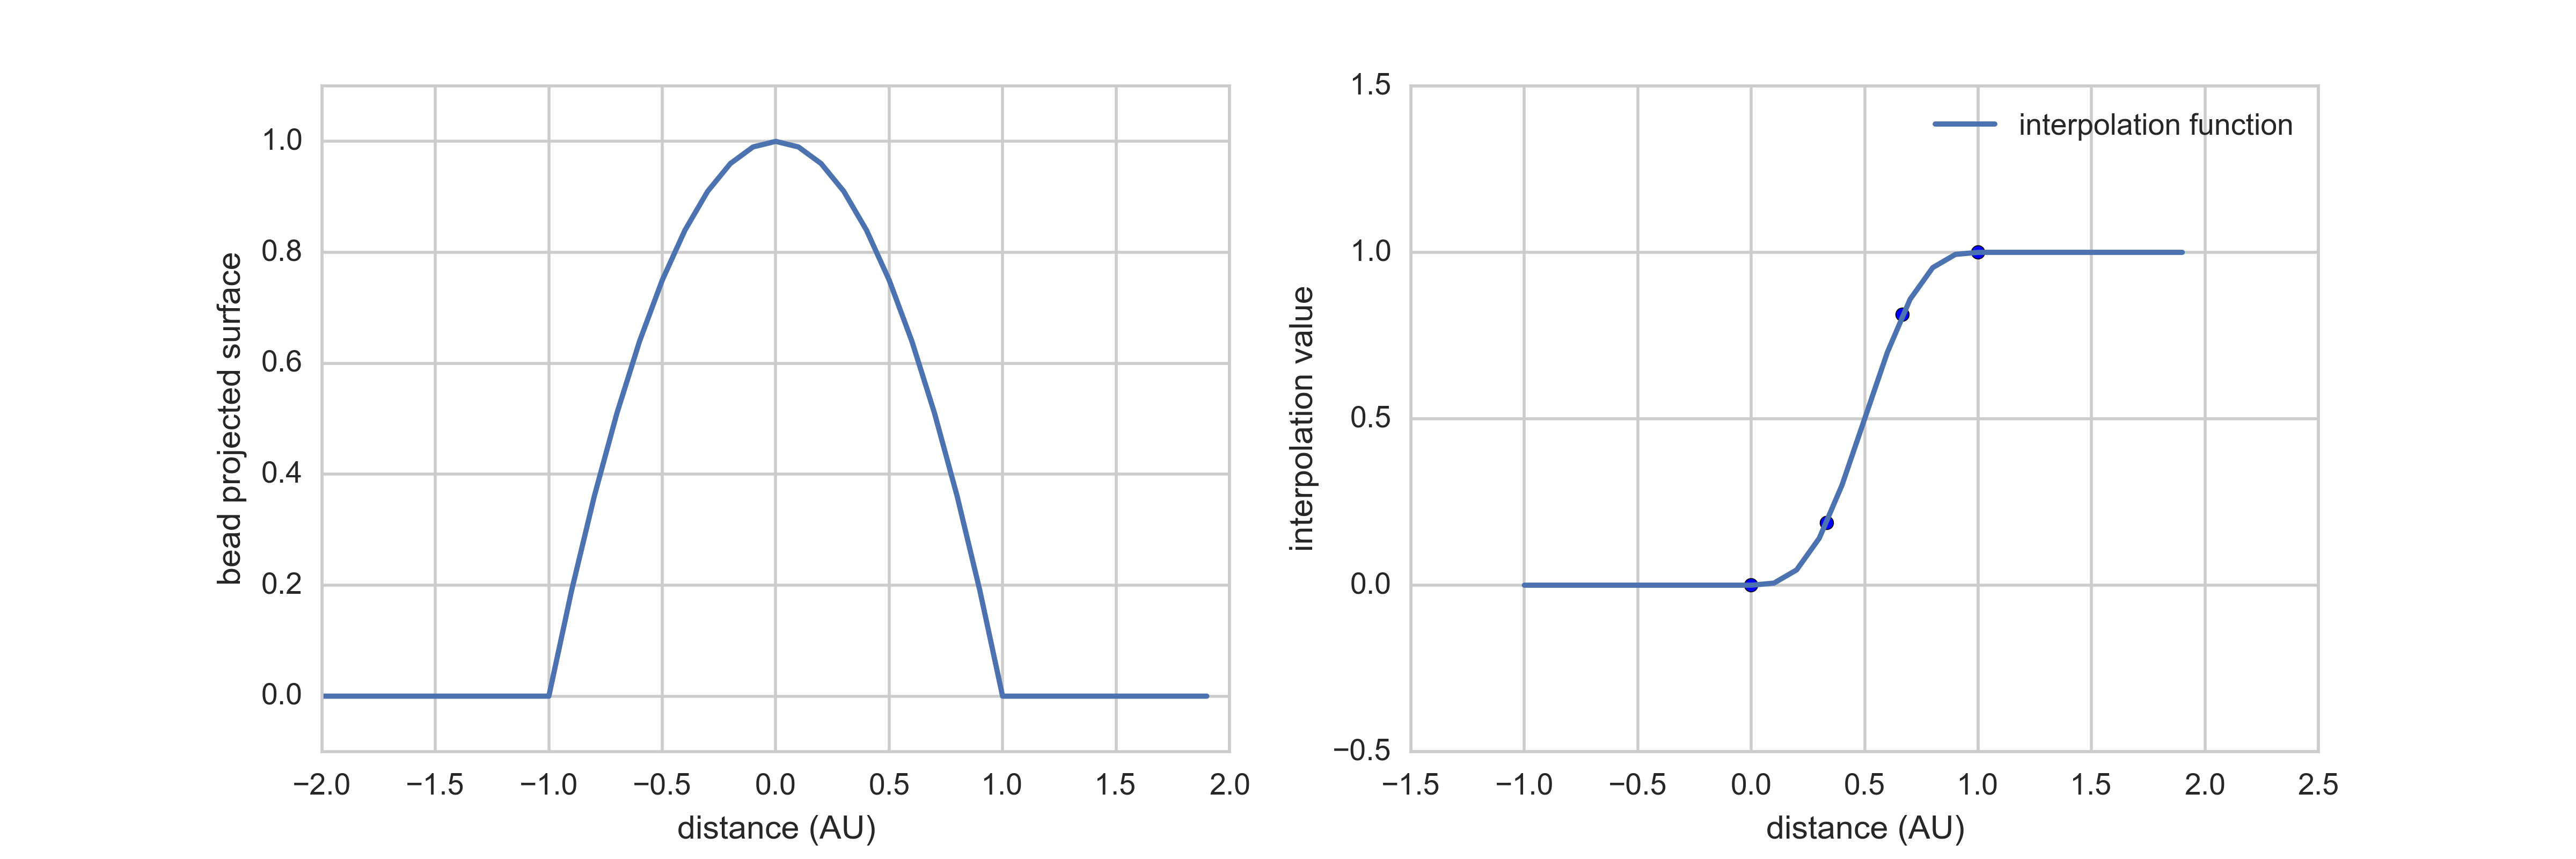
\includegraphics[width=0.900\linewidth]{interpolation.png}
\caption{Interpolation function used to smooth the transition from \(F_{da}\) to
\(F_{da}+F_{plaw}\)}\label{index-latex:interp}\end{figure}

The complete retraction force can be seen on \hyperref[index-latex:fit-3-phases]{figure  \ref*{index-latex:fit-3-phases}} and is equal to
\phantomsection\label{index-latex:equation-eqa314}\begin{gather}
\begin{split}F_{ret}(d) &= F_{da}(d)\times(1-S(d)) + F_{plad}(d)\times S(d)\\\end{split}\label{index-latex-eqa314}
\end{gather}
where \(S(d)\) is the interpolation function for a 4.34 µm
diameter bead. We can notice that the model correctly represents the retraction and especially
the position and value of the retraction function minimum without
fitting parameters, when using the probe-bead diameter as a typical scale
for the transition when changing direction.


\section{Discussion}
\label{index-latex:discussion}
The actin cytoskeleton plays an important role in many cellular functions.  The
actin cortex, just beneath the cell membrane is not only a crucial structure
for both cell motility and cell mechanical properties, it is also an essential
component in cell division and spindle positioning.  Other actin structures,
that spawn from the nucleus to the cell membrane, are responsible for cell
organelle positioning, as is the case for plants, where the nucleus is found
towards the cell anticlinal wall {\hyperref[index-latex:iwabuchi2010]{{[}Iwabuchi et al. 10{]}}}, or during nurse cell
maturation, where the nucleus is pushed away from the dumping
channel:cite:\emph{Huelsmann2013}. The mechanical link from the outside of the cells
to the nucleus using actin bundles has already been shown {\hyperref[index-latex:jaalouk2009]{{[}Jaalouk et al. 09{]}}}.
We demonstrated here that these actin structures should not be the only ones
taken into account to explain organelles positioning.

Our experiments confirmed the existence of a sparse and stiff actin cloud emanating
from a biomimetically reconstituted actin cortex.  This actin cloud is capable
of staining forces of tens of pico Newtons, enough to hold organelles in place. By using polymer physics,
we are able to model the behaviour of such an actin cloud and
to measure many of its mechanical properties. It provides an
actin scaffold capable of deforming non-plastically. At time scales of few
seconds it behaves mostly elastically with an elastic module of a few Pascal.
The actin cloud Poisson’s ratio varies from 0.1 to 0.2, hinting at a
sparse structure of loosely entangled filaments, forming a meshwork with a
typical mesh size of 300 to 400 nm.

The filaments at the origin of this loosely entangled network could emanate
from the dense actin cortex that can be seen and simulated on actin-beads
{\hyperref[index-latex:kawska2012]{{[}Kawska et al. 12{]}}} and the evolution of this actin cloud parameters are is
coherent with the preceding studies on biomimetically reconstituted actin
cortices. Recently, the role of actin networks with the same properties as an
actin cloud have been described in cells such as \emph{Xenopus} Oocyte
{\hyperref[index-latex:feric2013]{{[}Feric et al. 13{]}}}. The Poisson’s ratios of actin networks have been measured in
bulk to be higher {\hyperref[index-latex:gardel2003]{{[}Gardel et al. 03{]}}} but are not inconsistent with our
measurements at lower actin concentration.

The actin cloud provides a novel structure that should be studied further to
understand the positioning of organelles in cells, and to study the role this sparse
actin structure plays in the formation of other actin networks inside cells.

In particular, microrheology experiments could be performed on the growing actin
cloud in order to further characterise the frequency dependence of the actin cloud mechanical
properties. The effect of cross linking and network
branching is crucial for the occurrence of symmetry breaking on bead systems, and
probably plays a role in the actin cloud structure. A confined
geometry and direct polymerisation on membranes, or the effect of myosin motors
might alter the actin cloud properties.

All these, could be cellular mechanisms to use the actin cloud in order
to efficiently form the structures needed for its function.
Further studies of the actin cloud on biomimetic or \emph{in vivo} systems are
challenging, but would lead to a better understanding of the cells mechanics
and its control.

A Paper based on this study has been accepted for publication in Biophysical
Journal and is added for information as appendix of this manuscript.


\chapter{Cortical tension measured on liposome doublets}
\label{index-latex::doc}\label{index-latex:cortical-tension-measured-on-liposome-doublets}\label{index-latex:lib-doub}

\section{Introduction}
\label{index-latex:introduction}
We have seen that in cells, the actin cytoskeleton is a key component to form
structures such as the actin cortex, used to transmit forces and bring to cells
their mechanical rigidity. In order to drive shape changes, cells regulate the
mechanical properties of the sub-micrometer thick actin cortex,
beneath the membrane {\hyperref[index-latex:clark2013]{{[}Clark et al. 13{]}}}. The actin cortex dynamics
drives cell shape changes {\hyperref[index-latex:salbreux2012b]{{[}Salbreux et al. 12{]}}} and the presence of the
molecular motor myosin II plays a fundamental role in the tension of the
acto-myosin cortex {\hyperref[index-latex:tinevez2009]{{[}Tinevez et al. 09{]}}}. The cortical tension can be measured on
cells and varies between 50 and 4000 pN/µm in accordance with both actin and myosin activity .

These changes of the cortical tension are also affected by cell-cell
adhesions {\hyperref[index-latex:maitre2012]{{[}Maitre et al. 12{]}}} whose major role played in cell sorting have already been proved.

Recently, such acto-myosin cortices have been reconstructed on cell-sized
liposomes {\hyperref[index-latex:carvalho2013a]{{[}Carvalho et al. 13a{]}}}, which showed that the attachment of the actin
cortex to the membrane plays a crucial role in the acto-myosin network behavior and contractility.

In the present study, I collaborated with Kévin Carvalho and Joël Lemière, to
further extend the previously developed system {\hyperref[index-latex:carvalho2013a]{{[}Carvalho et al. 13a{]}}}
aiming at monitoring the cortical tension changes in a biomimetic actin cortex formed
on liposomes. I mainly contributed to the analysis of the 3D data, acquired by using Spinning Disk Microscopy and , for the analysis developed for this purpose a
novel method to get a precise and unbiased measure of the geometrical
parameter.

It should be noticed that in a recent works, cell doublets were used to determine the role of cortical tension in cells {\hyperref[index-latex:maitre2012]{{[}Maitre et al. 12{]}}}. In the present case, we formed similar doublets from liposomes,
around which we polymerised an actin cortex \emph{in vitro} (\hyperref[index-latex:fig1a]{Fig  \ref*{index-latex:fig1a}}). The
shape changes of these liposome doublets allowed the time-dependent monitoring of
cortical tension in a non-invasive way.  In this project, we hence developed a
method for the precise acquisition of doublet deformation, in order to accurately determine
the tension increase induced by the injection of myosin motor on
the preformed actin cortex.


\section{Experimental description}
\label{index-latex:experimental-description}

\subsection{Formation of liposomes doublets}
\label{index-latex:formation-of-liposomes-doublets}
Liposomes were obtained by electro-formation (see {\hyperref[index-latex:electroformation]{\emph{Material and methods}}} (\autopageref*{index-latex:electroformation})) from a mix of EPC and PEG-biotin lipids. The presence of
streptavidin in the working buffer allowed liposomes to naturally stick together
to form doublets after 15 minutes (\hyperref[index-latex:fig1a]{Fig  \ref*{index-latex:fig1a}}).
\begin{figure}[htbp]
\centering
\capstart

\includegraphics[width=0.500\linewidth]{Fig_01-A.png}
\caption{Cell-sized liposome doublets. Doublets are indicated by white arrows in
the field of view of a phase contrast microscope.}\label{index-latex:fig1a}\end{figure}


\subsection{Formation of actin cortex on doublets}
\label{index-latex:formation-of-actin-cortex-on-doublets}
The formation of the actin network on doublets was done in a similar way as recently described
{\hyperref[index-latex:carvalho2013a]{{[}Carvalho et al. 13a{]}}}.  Briefly, actin filaments including
biotinylated monomers were stabilised by phalloidin and linked to PEG-Biotin
lipids (see {\hyperref[index-latex:m-et-m]{\emph{materials and methods}}} (\autopageref*{index-latex:m-et-m}))  via streptavidin,
present in the solution (\hyperref[index-latex:fig1b]{Fig  \ref*{index-latex:fig1b}}).  Besides linking the actin to the
membrane, it also cross-linked the filaments.  Such a network has already been
recently characterised {\hyperref[index-latex:carvalho2013a]{{[}Carvalho et al. 13a{]}}}.  Note that as the actin filaments
were only added after the formation of the doublets, the interface between the
two liposomes composing the doublets remained free of F-actin (\hyperref[index-latex:fig1c]{Fig  \ref*{index-latex:fig1c}}, \hyperref[index-latex:fds]{ \ref*{index-latex:fds}}). As the added actin was fluorescent, the absence of actin
at the liposome interface could be checked by epifluorescence, as it appeared dark
compared to the rest of the doublet(\hyperref[index-latex:fig1c]{Fig  \ref*{index-latex:fig1c}}).
\begin{figure}[htbp]
\centering
\capstart

\includegraphics[width=0.700\linewidth]{doublets-schema.png}
\caption{Formation of doublets: 1) In the presence of streptavidin, single liposome
(A) aggregates into doublets. (B) The addition of biotinylated actin
filaments stabilized with phalloidin (2) forms liposome doublets covered
with a micrometer-sized actin network (C). The interface between the two
liposomes is a double lipid bilayer free of actin filaments.}\label{index-latex:fds}\end{figure}
\begin{figure}[htbp]
\centering
\capstart

\includegraphics[width=0.500\linewidth]{Fig_01-B.png}
\caption{Schematic of the stabilized actin cortex at the membrane (proteins not to scale).}\label{index-latex:fig1b}\end{figure}


\subsection{Visualisation of the interface}
\label{index-latex:visualisation-of-the-interface}\begin{figure}[htbp]
\centering
\capstart

\includegraphics[width=0.500\linewidth]{Fig_01-C.png}
\caption{i) Flow-chamber designed for buffer exchange. Doublets
are visualised in the middle horizontal channel of the H-shaped chamber to
avoid movements during the buffer exchange. Spinning disk images of the
doublet before i) or after iii) myosin II injection. One liposome contains the fluorophore
SRB (red) to visualise the doublet interface. The actin cortex is
labeled in green. Scale bar 5µm.}\label{index-latex:fig1c}\end{figure}

In order to visualise the interface between the liposomes, and to avoid the use of fluorescent
lipids that might affect the membrane mechanics, {\hyperref[index-latex:sandre1999]{{[}Sandre et al. 99{]}}} the inside
buffer of approximately half of the liposomes was labeled with 0.9 µM
of sulphorhodamin B (SRB
eventually leading to half of the doublets containing a single fluorescent liposome (\hyperref[index-latex:fig1c]{Fig  \ref*{index-latex:fig1c}} i and iii).


\subsection{Geometrical parameters}
\label{index-latex:geometrical-parameters}
To study the doublet geometry, we modelled each liposome and the interface
between them as two spherical caps with their respective center and radius, as
sketched in \hyperref[index-latex:fig-notations-doublets]{figure  \ref*{index-latex:fig-notations-doublets}}.
\begin{figure}[htbp]
\centering
\capstart

\includegraphics[width=0.500\linewidth]{notations-doublets.png}
\caption{The parameters notation for the doublet model: \(R_1\), \(R_2\), \(R_i\) are respectively the
radius of the liposome 1, the liposome 2 and the interface. \(d\) is the
distance between the liposomes centers. \(\theta_1\) and \(\theta_2\) are the angles between
the tangents of the liposome surface and the tangent to the interface at the
contact line. The total contact angle \(\theta\) is the sum of \(\theta_1\) and \(\theta_2\).}\label{index-latex:fig-notations-doublets}\end{figure}

The center position in 3D (X,Y,Z) and the radius (R) of the three spherical caps
completely determine the doublet geometry, though it is interesting to consider the other
parameters of the doublets, which are :
\begin{itemize}
\item {} 
the total volume of the liposome doublets \emph{V}

\item {} 
the contact angle between the two liposomes

\item {} 
Every ``half''-contact angles which are the angles between the
interface and each liposome \(\theta_1,\theta_2\)

\item {} 
The distance between the liposome centers.

\end{itemize}


\section{Experimental Observations}
\label{index-latex:experimental-observations}

\subsection{Effect of myosin-II injection}
\label{index-latex:effect-of-myosin-ii-injection}
We imaged the liposomes doublets in an open chamber either in phase contrast
and epifluorescence, or spinning disk microscopy in the red (sulphorhodamin)
and the green (actin) channel.

The muscle Myosin II that formed {\hyperref[index-latex:myoii]{\emph{bipolars filaments}}} (\autopageref*{index-latex:myoii}) was carefully injected into
the chamber, and led within a few minutes to a shape change (\hyperref[index-latex:doublets-contraction]{Fig  \ref*{index-latex:doublets-contraction}})
of the doublets, due to the actin cortex contraction.
\begin{figure}[htbp]
\centering
\capstart

\includegraphics[width=0.300\linewidth]{doublet-contract.png}
\caption{Doublets contraction showing a green channel(actin): (A) doublet before
myosin II injection. (B) doublet during contraction due to myosin II. Time=0 corresponds to myosin II injection.
Scalebar is 5 µm}\label{index-latex:doublets-contraction}\end{figure}

The distance between the liposome centers decreased as the total angle \(\theta
= \theta_1+\theta_2\) increased. The contact angle and other doublets parameters were obtained by fitting spherical caps onto the 2D epifluorescence
images or on the 3D confocal stack as {\hyperref[index-latex:full3dfit]{\emph{described later}}} (\autopageref*{index-latex:full3dfit}).  In the absence of myosin, the
contact angle \(\theta\) was measured to be \(\theta = 64 \pm 16 ^{\circ}\) (n=18), whereas in
the presence of myosin II (200 nM) we found  a value of \(\theta = 86 \pm 21
^{\circ}\) (n=5). Measurements of the contact angle after myosin II injection were done before the cortex
ruptures as characterised in {\hyperref[index-latex:carvalho2013a]{{[}Carvalho et al. 13a{]}}}.


\subsection{Relation between the angles and tension}
\label{index-latex:relation-between-the-angles-and-tension}
Each liposome has its respective tension \(\tau_1\), and \(\tau_2\).  In the absence
of the biomimetic acto-myosin cortex, these tensions only correspond to the
tension of the liposome membrane. The interface between the two liposomes is
formed by two lipid bilayers, and the inter-facial tension is composed of two contributions:
the tension of the lipid bilayer, noted \(\tau_i\), and the
adhesion energy per surface unit \(W\) due to the biotin-streptavidin-biotin link
between the two lipid bilayers. The total tension at the interface can thus be
written \(\tau_t = \tau_i -W\) {\hyperref[index-latex:maitre2012]{{[}Maitre et al. 12{]}}}.

As the movement of the contact line during the contraction is slow (order of
µm/min) compared to the pressure equilibration across the doublet, we can consider
the contact line between the liposomes and the interface to be at equilibrium.
Hence, we can apply Young's equation:
\phantomsection\label{index-latex:equation-eqa401}\begin{gather}
\begin{split}\sum_{k \in interfaces} \tau_k. \vec t_k  = \vec 0 \\
\tau_i \vec t_i + \tau_1 \vec t_1 + \tau_2 \vec t_2 + = \vec 0\end{split}\label{index-latex-eqa401}
\end{gather}
In which \(t_k\) are the vectors tangent to the interface at the contact point, as described in \hyperref[index-latex:fig-yd]{figure  \ref*{index-latex:fig-yd}}
\begin{figure}[htbp]
\centering
\capstart

\includegraphics[width=0.600\linewidth]{yd.png}
\caption{Equilibrium of the contact line. Each interface pulls on the line with a
force proportional to its tension. As the contact line is at equilibrium,
the sum of the forces compensate, thus ensuring  a relation between the tensions and the contact angles.}\label{index-latex:fig-yd}\end{figure}

This allows
to relate the tension of all the lipid layers and the angle
between them at each instance of the contraction. We can in particular project
the result of this equation onto the direction of the contact surface
tangent (dotted line on \hyperref[index-latex:fig-yd]{figure  \ref*{index-latex:fig-yd}}):
\phantomsection\label{index-latex:equation-young-tangent}\begin{gather}
\begin{split}\tau_i - W = \tau_1.cos(\theta_1) + \tau_2.cos(\theta_2)\end{split}\label{index-latex-young-tangent}
\end{gather}
And on the direction perpendicular to it :
\phantomsection\label{index-latex:equation-young-perpendicular}\begin{gather}
\begin{split} \tau_1.sin(\theta_1) = \tau_2.sin(\theta_2)\end{split}\label{index-latex-young-perpendicular}
\end{gather}
These equations link the tension to the contact angle before, during and
after the contraction and hence remain correct during the experiment. In the following, we will mark the values
before the contraction phase by
the suffix \emph{0}. Thus, for example \(\tau_{i,0}\) refers to the
interface tension before the addition of myosin, and \(\tau_i\) refers to the
interface tension at any instant of the contraction.


\subsection{Contact angle dispersion}
\label{index-latex:contact-angle-dispersion}
The value of the contact angle \(\theta\) varies across the different doublets both before
and after the  addition of myosin II. This reflects the initial variations of tension in
\(\tau_{i,0}\), \(\tau_{1,0}\), and \(\tau_{2,0}\) from doublet to doublet. Such variations could be
due to a difference in the liposome tension acquired during the different preparations, but also to a
variation of adhesion energy between doublets, or alternatively to an effect of tension build-up
during the actin shell formation. As the dispersion in the contact angle is
in the same order as the increase in the angle upon addition of myosin, a
statistical analysis of the contact angle before and during contraction is
problematic. Thus, to avoid this effect of dispersion, we followed the evolution of
\(\theta\) each individual doublet over time.


\subsection{Tension of actin-shell}
\label{index-latex:tension-of-actin-shell}
In order to investigate the tension increase due to the acto-myosin network
on liposomes, we first characterised the increase, only due to the addition of the actin-shell in
the absence of myosin. By destroying the F-actin via photo-bleaching (\hyperref[index-latex:fig2a]{Fig  \ref*{index-latex:fig2a}}) we compared the shape of the
same doublets in presence and absence of the actin-shell. It should be noted that it is established that the
actin filaments are destroyed by bleaching, as this process frees oxygen radicals that denature the actin monomers. Hence, the bleaching process
actually destroys the actin cortex ({\hyperref[index-latex:vandergucht2005]{{[}vanderGucht et al. 05{]}}}).
This investigation showed that the total contact
angle changes by \(3.4 \pm 2.0 ^{\circ}\) (n=7) after disruption (\hyperref[index-latex:fig2b]{Fig  \ref*{index-latex:fig2b}}) of the actin network.
Thus, we concluded that the tension change due of the actin-shell is negligible
compared to the tension change we can observe with myosin.
\begin{figure}[htbp]
\centering
\capstart

\includegraphics[width=0.500\linewidth]{Fig_02-A.png}
\caption{Image of an individual doublet coated with fluorescent F-actin before i) ii) and
after iii) iv) actin cortex disruption. The actin cortex is visualised by
epifluorescence ii) iv) and the doublet by phase contrast i) iii). Scale
bar 5µm.}\label{index-latex:fig2a}\end{figure}
\begin{figure}[htbp]
\centering
\capstart

\includegraphics[width=0.500\linewidth]{Fig_02-B.png}
\caption{Measurement of the contact angle between the two liposomes forming the
doublet before (black) and after (white) disruption of the stabilised actin
cortex as a function of their volume.}\label{index-latex:fig2b}\end{figure}


\section{3D observation}
\label{index-latex:d-observation}\label{index-latex:d-obs}
The three dimensional imaging of the doublets is necessary to get the correct
contact angle. This requirement comes from the fact that in simple 2D epifluorescence
images, the focal plane would have to correspond to the equatorial plane of the doublets for correct analysis. If
this is not the case, the fit will produce a systematic underestimation of the contact angle.
This is especially the case when doublets are of different radii, as typically found in our
experiments, where the liposomes composing the doublets have an ratio of \(R_1 / R_2\) between 1.15 and 1.82.
\begin{figure}[htbp]
\centering
\capstart

\includegraphics[width=0.900\linewidth]{light_table.png}
\caption{Confocal stack of a liposome doublet actin channel, 3D reconstruction in
\hyperref[index-latex:fig3a]{figure  \ref*{index-latex:fig3a}}. Note that there is no actin at the interface between
the liposomes (Frames \#11-\#14). The distance between each image is \(\Delta z=0.85\) µm.}\label{index-latex:confocal-stack}\end{figure}
\begin{figure}[htbp]
\centering
\capstart

\includegraphics[width=0.500\linewidth]{Fig_03-A.png}
\caption{3D reconstruction of a doublet surrounded by actin. The absence of actin on
the interface can be more easily observed on \hyperref[index-latex:confocal-stack]{figure  \ref*{index-latex:confocal-stack}}.}\label{index-latex:fig3a}\end{figure}

Time resolved 3D Spinning disk stacks (\hyperref[index-latex:confocal-stack]{Fig  \ref*{index-latex:confocal-stack}} with 3D reconstruction
\hyperref[index-latex:fig3a]{Fig  \ref*{index-latex:fig3a}}) are recorded with a time resolution of less than 5 seconds per stack, for an accurate determination of the different
doublet parameters over time. The analysis reveals the contact angle \(\theta\) (\hyperref[index-latex:fig3b]{Fig  \ref*{index-latex:fig3b}}) , the
doublet volume \(V\) (\hyperref[index-latex:fig3d]{Fig  \ref*{index-latex:fig3d}}) and the distance between liposome
centers \(d\) (\hyperref[index-latex:fig3c]{Fig  \ref*{index-latex:fig3c}}). All these parameters are obtained by
fitting spherical 3D caps on the 3D stack as explained {\hyperref[index-latex:full3dfit]{\emph{later}}} (\autopageref*{index-latex:full3dfit}).
\begin{figure}[htbp]
\centering
\capstart

\includegraphics[width=0.500\linewidth]{Fig_03-B.png}
\caption{Evolution of the contact angle compared to its initial value as a function of
time.  Each doublet is represented by a different color. The color code corresponds to the doublet
shown in figure \hyperref[index-latex:fig3c]{ \ref*{index-latex:fig3c}}, \hyperref[index-latex:fig3d]{ \ref*{index-latex:fig3d}}
and \hyperref[index-latex:fig3e]{ \ref*{index-latex:fig3e}}. A special case is highlighted in the blue dashed line,
where the actin cortex on the doublet ruptured, and the cortex is peeled off.
The analysis of this case showed that the contact angle after rupture recovers its initial value.}\label{index-latex:fig3b}\end{figure}
\begin{figure}[htbp]
\centering
\capstart

\includegraphics[width=0.500\linewidth]{Fig_03-C.png}
\caption{Evolution of the distance between liposome centers as a function of time.
Same color code for same doublets as in figure \hyperref[index-latex:fig3b]{ \ref*{index-latex:fig3b}}, \hyperref[index-latex:fig3d]{ \ref*{index-latex:fig3d}}
and \hyperref[index-latex:fig3e]{ \ref*{index-latex:fig3e}}. Again, the doublet with the ruptured cortex recovers its initial parameter values.}\label{index-latex:fig3c}\end{figure}
\begin{figure}[htbp]
\centering
\capstart

\includegraphics[width=0.500\linewidth]{Fig_03-D.png}
\caption{Evolution of the volume ratio over time.
Same color code for same doublets as in figure \hyperref[index-latex:fig3b]{ \ref*{index-latex:fig3b}}, \hyperref[index-latex:fig3c]{ \ref*{index-latex:fig3c}}
and \hyperref[index-latex:fig3e]{ \ref*{index-latex:fig3e}}.}\label{index-latex:fig3d}\end{figure}

During the contraction triggered by myosin, we observed that the contact angle
\(\theta\) increased while the distance between liposome centers \(d\) decreased.
During this process, the volume remained constant within the error rate? of 10\%.  These
results are consistent with the contact angle measures in freely adhering cell
doublet experiments done previously {\hyperref[index-latex:maitre2012]{{[}Maitre et al. 12{]}}}.


\section{Discussion}
\label{index-latex:discussion}

\subsection{Cortical tension is homogeneous for single doublet}
\label{index-latex:cortical-tension-is-homogeneous-for-single-doublet}
Combining the equation \eqref{index-latex-young-perpendicular} with the finding that \(\theta_1 = \theta_2 = \theta
/2\), allows to infer the equality of tension on both sides of the doublet during all the
experiments. We can hence write \(\tau_1 = \tau_2 = \tau\). This result is
consistent with the fact that actin is continuously distributed all around the
liposome doublet. Hence, myosin II minifilaments pull on a continuous shell. In
these conditions, equation \eqref{index-latex-young-tangent} simplifies to :
\phantomsection\label{index-latex:equation-eq3}\begin{gather}
\begin{split}\tau_i - W = 2.\tau(t).cos(\theta(t)/2)\end{split}\label{index-latex-eq3}
\end{gather}
Where \(\tau(t)\) and \(\theta(t)\) are the tension and the angle at
time \(t\)  after myosin injection. That
\(\tau_i-W\) may depend on a variability of the initial adhesion between
liposomes. Since myosin does not operate at the interface between liposomes as
it is actin-free, we can reasonably consider that both the tension and
the adhesion energy are constant for a given doublet over time
\(\tau_i-W = \tau_{i,0}-W_0\).
Therefore, we obtain an expression of the tension \(\tau(t)\) during the acto myosin contraction that reads :
\phantomsection\label{index-latex:equation-eqtime}\begin{gather}
\begin{split}\tau(t) &= \frac{ \tau_i - W }{2.cos(\theta/2)}\\
        &= \frac{ cst           }{2.cos(\theta/2)}\end{split}\label{index-latex-eqtime}
\end{gather}
Consequently, we can evaluate the tension relative to its initial value over time :
\phantomsection\label{index-latex:equation-eqa402a}\begin{gather}
\begin{split}\frac{ \tau(t) }{\tau_0} = \frac{cos(\theta_0/2)}{cos(\theta(t)/2)}\end{split}\label{index-latex-eqa402a}
\end{gather}

\subsection{Relative increase in cortical tension}
\label{index-latex:relative-increase-in-cortical-tension}
The interaction of myosin II filaments with a biomimetic actin cortex induces
tension build-up. The cortical tension, normalised to its initial value,
increases and reaches a plateau where \(\tau(t) = \tau_{peeling}\)
(\hyperref[index-latex:fig3e]{Fig  \ref*{index-latex:fig3e}}), with the same trend as \(\theta\).  Note that if the acto-myosin shell
breaks and peels, the doublet recovers its initial shape (see dashed blue line
for \(d\) and \(\theta\) on  \hyperref[index-latex:fig3b]{Fig  \ref*{index-latex:fig3b}}, \hyperref[index-latex:fig3c]{ \ref*{index-latex:fig3c}}, \hyperref[index-latex:fig3d]{ \ref*{index-latex:fig3d}} ). The average relative tension is found to
be \(\tau_{peeling}/\tau_0 = 1.56 \pm 0.56\) (n=5) in 3D and
\(\tau_{peeling}/\tau_0  = 1.25 \pm 0.15\) (n=5) in epifluorescence, in
agreement with the discussed expected underestimation of the contact angle in epifluorescence measurements.
\begin{figure}[htbp]
\centering
\capstart

\includegraphics[width=0.500\linewidth]{Fig_03-E.png}
\caption{Increase of the tension ratio between the tension \(\tau(t)\) at time
\(t\) and the initial one \(\tau_0\).
Same color code for same doublets as in figure \hyperref[index-latex:fig3b]{ \ref*{index-latex:fig3b}}, \hyperref[index-latex:fig3c]{ \ref*{index-latex:fig3c}}
and \hyperref[index-latex:fig3d]{ \ref*{index-latex:fig3d}}. The actin cortex rupture in the blue dashed line also presents the highest relative tension increase.}\label{index-latex:fig3e}\end{figure}


\subsection{Cortical tension increase in doublets and in cells}
\label{index-latex:cortical-tension-increase-in-doublets-and-in-cells}
In cells, the cortical tension can be as low as 50 pN/µm in fibroblast progenitor
cells {\hyperref[index-latex:krieg2008]{{[}Krieg et al. 08{]}}} and can go up to 4000 pN/µm for
dictyostelium {\hyperref[index-latex:schwarz2000]{{[}Schwarz et al. 00{]}}}. Surprisingly, when myosin activity is
affected, either by drugs or by genetic manipulation, the cortical tension only
decreases by a factor of about 2. Cells are also observed to round up during
division, where a  tension increase by a factor of two
is sufficient {\hyperref[index-latex:stewart2011]{{[}Stewart et al. 11{]}}}, {\hyperref[index-latex:kunda2008]{{[}Kunda et al. 08{]}}} .
Our \emph{in vitro} reconstruction is able to reproduce similar
changes of cortical tension, as we observe a cortical tension increase by a factor of up to 2.4.


\subsection{Different contributions for cortical tension}
\label{index-latex:different-contributions-for-cortical-tension}
The cortical tension is the sum of the membrane tension and the tension due to the
acto myosin cortex. We questioned how the membrane could contribute to the cortical tension
and in our assay, we showed that in some cases, it might account for approximately 50\% of the cortical tension.
In suspended fibroblast cells, the membrane tension is estimated to amount to 10\% of the
cortical tension {\hyperref[index-latex:tinevez2009]{{[}Tinevez et al. 09{]}}}. When the actin polymerisation is
stimulated, the cortical tension is multiplied by a factor of 5, also showing a
strong dependence with actin dynamics {\hyperref[index-latex:tinevez2009]{{[}Tinevez et al. 09{]}}}. Therefore, the
residual tension in cells might be due to actin dynamics, which is absent in our
experiments. How actin contributes to cortical tension is still an open question
that needs to be addressed to the cell geometry.  Whereas it has been proved that actin polymerisation
outside a liposome generated inward pressure,
the way this observation can be translated into tension  in a different geometry is
not yet clear. \emph{In vitro} assays are on their way to mimic actin dynamics in
cells {\hyperref[index-latex:abushah2014]{{[}AbuShah et al. 14{]}}}. They will allow to unveil the mechanisms of tension build-up by
actin dynamics, the last remaining module that still needs to be understood,
as the effect of both myosin and membrane have been clarified in this study.


\subsection{Conclusion}
\label{index-latex:conclusion}
We provided a biomimetic reconstitution of the tension build-up by acto-myosin
contractility, through the use of liposome doublets. Cortical tension changes were visualised
\emph{in situ} over time by analysing doublet shape changes. This method allowed us
to directly quantify the relative increase in tension due to myosin,
regardless of the one due to actin dynamics. So, a thorough understanding of the composite systems contraction,
rebuilt brick by brick to finally model a living cell, will hopefully lead the way towards a reconstitution
of complex systems like tissues.


\section{3D fitting}
\label{index-latex:full3dfit}\label{index-latex:d-fitting}
It remains challenging to obtain the doublets geometrical parameter, as in
classical phase contrast and epifluorescence microscopy, the acquired images
only capture a single focal plane of the doublets. This makes the analysis
difficult, as the observation plane should be the
equatorial plane of the doublet.

In order to achieve a good precision in the measurements of the contact angle, we
decided to use confocal microscopy and to acquire evenly spaced z-stacks. The doublets 3D structure was reconstituted
from these stacks,  thus allowing to recover the geometrical parameters and
the contact angle.

In order to determine the geometrical doublets parameters,
we modelled them as two intersecting spheres, determined the expected 3D
images and adjusted the model parameters to resemble the obtained
experimental data.

I was responsible for developing a fast and precise method to reliably and
automatically recover the liposome doublets geometrical parameters,
based in the image stacks, acquired by using spinning disk microscopy. In the following part, I will develop the principle of this
method and the result on liposomes doublets.


\subsection{First step: Fitting a single liposome}
\label{index-latex:first-step-fitting-a-single-liposome}
In this part, we will describe the principle that allowed us to determine the 8
geometrical parameters that characterise a doublet: 2 centers (X,Y,Z) and 2 radii
(\(R_1\) and \(R_2\)).

As the principle for finding the geometrical parameters does not differ with the
number of dimensions, the presented methods can be applied even in higher dimensions (e.g. deformed
ellipsoid liposome, or multi channel imaging). Furthermore, as the principles also remain  similar in a
space with less dimensions, we will restrict our discussion to a single liposome
in a 2D plane (X,Y position of centers and R, radius, hence reducing the parameters to be determined to six instead of eight).

Experimentally, liposomes are observed using fluorescently labeled actin that
forms an homogeneous micrometer-sized actin shell. In the observation plane,
the liposome is a bright ring of a predetermined thickness (we will refer to this as the
\emph{expected signal}). We can observe the experimental noise on top of the image, where the
principal sources are identified as the presence of fluorescent actin monomers in the
buffer solution and electronic noise from the CCD camera.
Eventually, the noise in the outside buffer, due to monomeric actin, can be higher than in the inside buffer, which is actin-free.

The signal from a liposome and the addition of noise can be replicated
numerically as per \hyperref[index-latex:fig-2d-sim]{figure  \ref*{index-latex:fig-2d-sim}}.
\begin{figure}[htbp]
\centering
\capstart

\includegraphics{modl-2D-doublet.png}
\caption{Left : A simulation of liposome fluorescent image consisting of a uniform shell or membrane
(\emph{expected signal}).  Middle: Same Image Adding Gaussian noise. This simulates
one plane of a confocal Z-stack.  Right: Liposome simulation   with
a fluorescently labeled actin shell in a fluorescent external buffer and a non
fluorescent inside buffer.}\label{index-latex:fig-2d-sim}\end{figure}

The \emph{expected signal} can be modelled numerically, using several parameters of
the system (center and radius of liposome, point spread function of microscope,
...).

In order to find the correct parameters for the doublets, we will numerically correlate
the acquired data with the numerical model and search for the correlation
that best corresponds to the real image. The correlation between the model and the images
data can be. expressed as :
\phantomsection\label{index-latex:equation-eqa402}\begin{gather}
\begin{split}r_{xy}=\frac{\sum\limits_{i=1}^n (x_i-\bar{x})(y_i-\bar{y})}{(n-1) s_x s_y}\end{split}\label{index-latex-eqa402}
\end{gather}
In which \(x_i\) are the luminosity values of each \(n\) pixel in
the acquired data, \(y_i\) represent the pixels luminosity in the model
\(\bar{x},\bar{y}\) correspond to the average values over the images,
\(s_x\) and \(s_y\) are the standard deviation of the luminosity
values.

As the monomeric fluorescently labeled actin and the electronic noise are dominant
in the acquired images, we can assume a uniform noise on top of the \emph{expected signal}. The correlation between the model and the noise is on average
uniform.
.. math:

\begin{Verbatim}[commandchars=\\\{\}]
:label: eqa403

r\PYGZus{}\PYGZob{}noise,model(params)\PYGZcb{} = cst
\end{Verbatim}

And the correlation between the \emph{expected signal} and the model is expected to be
maximal for the model parameters  equivalent to the real geometrical
doublets parameters.
\phantomsection\label{index-latex:equation-eqa404}\begin{gather}
\begin{split}{arg\,max}_p\left(r_{data,model(p)}\right)= {arg\,max}_p \left(r_{expectedSignal,model(p)}\right)\end{split}\label{index-latex-eqa404}
\end{gather}
In which \({arg\,max}_p\) stands for the
argument of the maximum, that is to say, the set of points of the considered
argument, for which the given function reaches its maximum value. Thus, searching
for parameter values that maximise the correlation between the model and
the data, implies that we find the geometrical parameters we are interested in.

We can test the ability to do this numerically by generating data, adding noise
to it and trying to recover the parameters of the \emph{expected signal}.

By looking at the correlation value between the generated data and the model
as a function of model parameters, we can check that the correlation
values are maximal when the model center value corresponds to the \emph{expected signal}
center value (Fig \ref{index-latex:corr-fun-1}), and when the radius of the model liposome
has the same radius in the model and corresponds to the radius in the generated data (Fig \ref{index-latex:corr-fun-2}).
\begin{figure}[htbp]
\centering
\capstart

\includegraphics[width=0.500\linewidth]{double-c-_100-by-100-rc-40_0-noise-0_5-delta-4_0_.png}
\caption{Correlation value as a function (arbitrary units) of two among the fit
parameters. The liposome radius in the model is taken as
equal to the value of the \emph{expected signal}, and the position of the center
is varied?  in the X and Y directions. The correlation value is maximal for
the center position in the model, that equals to the center of the
\emph{expected signal}.  The local maxima observed on the 3D representation
are well below the global maximum value.
The peak at the global maxima is sharp, hinting that
the search of the maxima requires relatively good initial
parameters (lower than \textasciitilde{}1/10 of the liposome radius). The sharpness of the peak
point corresponding to the best fit parameters on experimental data, should be
robust.}\label{index-latex:corr-fun-1}\end{figure}
\begin{figure}[htbp]
\centering
\capstart

\includegraphics[width=0.600\linewidth]{c-R-_100-by-100-RC-40_0-noise-0_5-delta-4_0_.png}
\caption{Same as \hyperref[index-latex:corr-fun-1]{figure  \ref*{index-latex:corr-fun-1}}  with Y, center position taken
as equal to the expected signal, variating X position of the model and
radius of the liposome. The graph shows the same properties as before.}\label{index-latex:corr-fun-2}\end{figure}

We could search the parameter space of the model and
maximise the correlation between the model and the experimental data through the use of minimisation techniques. We then
could recover the liposomes geometrical parameters by
efficiently computing the correlation value within a few hundreds of
points, thus giving access to the liposomes' geometrical parameters, in this instance position
and radius.


\subsection{Fitting a doublet}
\label{index-latex:fitting-a-doublet}
The determination of the contact angle on epifluorescence images or phase contrast
images often results in an underestimation, as the imaging plane is not necessarily one of the doublets
equatorial planes. Moreover, most determinations of the contact angle on phase
contrast and epifluorescence images are handmade {\hyperref[index-latex:maitre2012]{{[}Maitre et al. 12{]}}} and
are subject to experimenter’s bias, as the experimenter draws the tangent lines at the
contact point between the liposomes. Thus, we decided to develop fitting routines for the acquired
3D confocal stacks. In our case, we avoided the usage of
fluorescent lipids that could artificially change the membrane tension.

As sketched in \hyperref[index-latex:fds]{figure  \ref*{index-latex:fds}}, the doublets are covered with a
thin micrometer-thick layer of fluorescent actin filaments, which we
imaged by confocal spinning disk microscopy. As the actin-layer is attached to the membrane
and the contact angle is defined as the angle between the lipid bilayer, imaging the actin-layer corresponded
to the angle between the inner surfaces of the two actin networks present on each liposome.

Thus, in order to determine the geometrical parameters of the doublets we also needed
to model the actin shell. As the liposomes in contact consist of two spherical
caps, the uniform actin layer will also form two spherical caps with a given
thickness. The total image is thus the union of two spherical caps blurred by
the point spread function of the microscope. This can be seen on \hyperref[index-latex:mproj1]{figure  \ref*{index-latex:mproj1}}.  We can notice on this image the presence of the doublet, lying on the
chamber surface. We checked in this case that the contact surface between the
chamber and the doublet did not change during experiments.
\begin{figure}[htbp]
\centering
\capstart

\includegraphics[width=0.800\linewidth]{max_proj_340A.png}
\caption{Maximum projection along X,Y and Z of recorded stacks, green channel represents actin.
One can observe that the liposome doublets are lying on the surface of the
observation chamber (arrows).}\label{index-latex:mproj1}\end{figure}

As the doublets contraction is rapid, and the recorded 3D stacks contain a
large number of frames, it is hence crucial to be able to compute the model and the
correlation in a reasonable time (less than an hour per images). To
achieve this besides calculating the model as efficiently as possible, one can
replace the exact calculation of two spherical caps and the point spread
function of the microscope by the union and subtraction of pre-calculated spheres followed by a 3D
numerical Gaussian blur (\hyperref[index-latex:fig-mdl]{Fig  \ref*{index-latex:fig-mdl}}).
\begin{figure}[htbp]
\centering
\capstart

\includegraphics[width=0.600\linewidth]{3dblur.png}
\caption{Principle of numerically approximating the two spherical caps as intersection of two spheres,
followed by a 3D numerical Gaussian blur. Compared to the exact calculation of the fluorescent density, the numerical speed-up allows
to make fits on doublets in minutes instead of hours.}\label{index-latex:fig-mdl}\end{figure}

However, the use of such numerical techniques is not devoid of artefacts.  In the particular case of
discreet Z-stacks that are not sufficiently spaced, the different radii in the
fluorescent rings within subsequent stacks can lead to a ``ring-artefact'' (\hyperref[index-latex:ring-artifact]{Fig  \ref*{index-latex:ring-artifact}}), when using numerical Gaussian blur. In the case of a too
pronounced ``ring-artifact'', a ``ghost'' spheres can appear around each liposome,
liable to cause the doublets fitting process to fall into a local
maximum of correlation, thus leading to a wrong value of the geometrical
parameters.
\begin{figure}[htbp]
\centering
\capstart

\includegraphics[width=0.700\linewidth]{ring_artifact.png}
\caption{Left : One plane of the numerical model with an exaggerated ring artifact due
to an under sampling of the model in the Z-direction, stacks from ``Far'' Z
leak onto the current Z-plane and forms a ring.  Right : Same model plane  with enough sampling plane in the Z-direction, does not show the ring
artefact. In this case, we used a sampling with the same number of slices than
the recorded data. (X,Y in arbitrary units)}\label{index-latex:ring-artifact}\end{figure}
\begin{description}
\item[{In our case, we had a sufficient number of planes per stack so that}] \leavevmode
the numerical model with the same sample size similar to the data, did not show the ring artefact and had

\end{description}

a smooth transition near the position of the spherical cap. Though, the ring
artefact could be eliminated by oversampling/interpolating the model before the
numerical Gaussian blur and undersampling afterwards to reach the correct number of
pixels.

The size of the
Gaussian blur, which will act as a regularisation
function for the value of the correlation between the model and the acquired
data, can also be adjusted to be higher (see \hyperref[index-latex:max-proj-model]{Fig  \ref*{index-latex:max-proj-model}}), thus smoothing or eliminating local maxima,
but reducing the precision in the maxima position.
\begin{figure}[htbp]
\centering
\capstart

\includegraphics[width=0.500\linewidth]{max_proj_model.png}
\caption{Maximum projection along the X,Y and Z of numerical model, the ``ring'' effect
is still slightly visible near the pole of each liposome, but is not
sufficient for the fit to be stuck in a local minimum.}\label{index-latex:max-proj-model}\end{figure}

The correlation value between the model and the experimentally recorded
data can be maximised, by using already available functions, and more particularly the Nelder–Mead simplex algorithm as implemented in \emph{scipy.optimise} python library. This
provided us with the 8 parameters of the doublets. Result of the fits are shown in
\hyperref[index-latex:fig-fit-t0]{figure  \ref*{index-latex:fig-fit-t0}}.
\begin{figure}[htbp]
\centering
\capstart

\includegraphics[width=0.500\linewidth]{Doublet-402-A-Fit-t-0.png}
\caption{Maximum projection of confocal images in the X,Y and Z projections as well
as the result of the fits shown as equatorial circles for the three
directions}\label{index-latex:fig-fit-t0}\end{figure}

of projection.

Using the fast Cython code ({\hyperref[index-latex:seljebotn2009]{{[}Seljebotn 09{]}}}) also allowed to speed
up fitting to a reasonable time: one Z-stack of 3 millions pixels can be fitted
in about 40 seconds, thus allowing the fitting of a full 3D movie of a doublets
contraction to be completed in less than an hour for 30 to 40 frames.

To ensure fits robustness to doublet center displacement during
acquisition, the initial parameter of the fit were chosen manually for each
first frame of each sequence. The final fit parameters of each frame are reused
as initial fit parameters for the subsequent frame.

In order to test the robustness of the fit, we randomly modified the initial fit parameters by +/- 1µm, and we checked that the final parameters did
not vary.

For a couple of parameters, the correlation function values can be plotted
to check the regularity of the function and the absence of local maxima. \hyperref[index-latex:gof2d]{Figure  \ref*{index-latex:gof2d}} and \hyperref[index-latex:gof3d]{figure  \ref*{index-latex:gof3d}} show the resulting correlation values.
\begin{figure}[htbp]
\centering
\capstart

\includegraphics[width=0.600\linewidth]{gof-2d-doublets.png}
\caption{Correlation of the model and the data as a function of the center position
of one of the model spherical caps along the X axis and the radius of this
same spherical cap. Vertical axis in arbitrary unit.}\label{index-latex:gof2d}\end{figure}
\begin{figure}[htbp]
\centering
\capstart

\includegraphics[width=0.600\linewidth]{gof-3d-doublets.png}
\caption{3D representation of the data in \hyperref[index-latex:gof2d]{figure  \ref*{index-latex:gof2d}}, the function shape is the same as the simulation done with the \emph{expected signal} in
\hyperref[index-latex:corr-fun-1]{figure  \ref*{index-latex:corr-fun-1}} \hyperref[index-latex:corr-fun-2]{and  \ref*{index-latex:corr-fun-2}}}\label{index-latex:gof3d}\end{figure}

The fit correctness is also checked visually to prevent errors in the
procedure.  We found that the fit was systematically accurate and coherent with the manual
measurements of the contact angle.  Whenever the red channel was also present and the liposomes
contained sulphorhodamin B, we were additionally able to visually check the fits, by using the maximum
projection of the red channel.  (see \hyperref[index-latex:srhod]{Fig  \ref*{index-latex:srhod}}).
\begin{figure}[htbp]
\centering
\capstart

\includegraphics[width=0.800\linewidth]{srhod_superimpose.png}
\caption{Maximum projection of the red channel (\emph{sulphorhodamin}) and fitted
parameter for the doublet.}\label{index-latex:srhod}\end{figure}


\subsection{Discussion}
\label{index-latex:id24}
This part aimed at demonstrating that by modelling the liposome doublet and using
fluorescently labeled actin, we were able to develop a technique that
automatically and robustly determined the geometrical properties of the liposome
doublets.

We noted that the red fluorescent dye present in the inside buffer of the
liposome could be used conjointly for the green channel, in order to improve the
fit quality, though this would require the extra parameters of the
interface radius. As the required computation time to fit the doublets increases
rapidly with the parameters number,
we came to the conclusion that this solution was impractical.  Moreover, the interface curvature is relatively small
and the difference between the curved interface and a flat plane close to
the optical resolution, hence the risk for the fits to become unstable.  The use of
fluorescently labeled lipids for the liposome membrane also suffers from the
same issues of extra parameters, if one wants to recover the interface position.


\subsection{Conclusion}
\label{index-latex:id25}
We developed a robust and automated method to determine the geometrical
parameters of liposome doublets. This allowed to robustly determine the
liposome doublets geometrical parameters without
any experimenter’s measurements bias, thanks to the selection of the illumination plane,
the resolution of optics and the luminosity scale.

We determined that liposome doublets with reconstituted acto-myosin cortices were
a biomimetic system allowing to measure the changes in cortical tension with
time. 3D fitting helped to quantify the tension by obtaining the corresponding contact angles.

A simultaneous observation of the contraction of multiple liposomes doublets and the
ability to automatically determine the geometrical parameters allowed the collection of more
samples. A faster and more reliable data acquisition on actin
network contractions will lead to a better understanding of the effect of actin
network \emph{in vitro} thus also paving the way for the reconstitution of more complex systems.


\chapter{Active cytoplasm movement in mouse oocytes}
\label{index-latex::doc}\label{index-latex:active-cytoplasm-movement-in-mouse-oocytes}

\section{Introduction}
\label{index-latex:introduction}
Mouse oocytes are big spherical cells with a diameter around 80 µm.  A previous work has established
that the spindle positioning during meiotic cell division in oocytes depends
on an actin meshwork present in the cell's cytoplasm {\hyperref[index-latex:schuh2008]{{[}Schuh et al. 08{]}}}.  This
actin meshwork is regulated by formin, localized to endogenous vesicles.
Additionally, these vesicles recruit the myosin-Vb motor proteins, that are known to drive the vesicles active movement
in the cytoplasm {\hyperref[index-latex:holubcova2013]{{[}Holubcova et al. 13{]}}}. In a collaborative project with the group of Marie-Hélène Verlhac
and her Postdoc Maria Almonacid at the Collège de France, I designed a way to measure the cytoplasmic activity in mouse oocytes.

\hyperref[index-latex:oocytewt]{figure  \ref*{index-latex:oocytewt}} presents a typical mouse
oocyte, where the nucleus can be seen positioned at the center of the cell.
In this system, current questions relate to the mechanical processes during meiosis such as the chromosome migration,
the asymmetric cell division and the organelles positioning by the dynamic remodelling of the actin network.
While our team did active and passive microrheology measurements on timescales of 10 seconds, I developed a
suitable method  for longer timescales in the order of minutes, more relevant for the meiosis process.
\begin{figure}[htbp]
\centering
\capstart

\includegraphics[width=0.600\linewidth]{oocyte-wild-type.png}
\caption{Bright field image of a mouse oocyte before meiosis (scale bar is 20 µm).
The cell diameter is about 80µm. The nucleus is positioned at the center of
the oocyte during meiosis with the help of the actin network. The
positioning is a crucial factor for the normal oocyte division. The
oocytes are a good reference system as they provide a clean spherical
symmetry and due to their size, give a good spatial difference between the
cortex and the cytosol, which helps to measure the spatial variations of
mechanical properties and vesicle movement. Image Credit to Maria
Almonacid, Collège de France.}\label{index-latex:oocytewt}\end{figure}


\section{Oocytes}
\label{index-latex:oocytes}
The cytosolic actin meshwork in oocytes is controlled by the activity of formins (Fmn2) that
nucleate actin polymerisation, and by the activity of the vesicle-bound molecular motor protein myosin Vb that
controls the dynamic movement of the
vesicles in the actin meshwork. Hence, it is of interest to study oocytes with formin and myosin Vb deficits.
We focused more particularly on three types: 1) Wild type oocytes, 2) oocytes prepared from Formin 2 invalidated female
(Fnm2-/-) that lacks the
actin meshwork and 3) oocytes injected with the RNA coding for the dominant-negative tail of Myosin
Vb (\hyperref[index-latex:fig3oo]{Fig  \ref*{index-latex:fig3oo}}), thus replacing the active myosin Vb on the vesicles.
\begin{figure}[htbp]
\centering
\capstart

\includegraphics[width=1.000\linewidth]{3-oocytes.png}
\caption{Bright field image microscopy of the 3 kinds of oocytes (Credit to Maria
Almonacid, Collège de France). WT) Image of Wild Type Oocyte, Scale bar is
20µm. Fmn2-/-) Oocytes extracted from females with invalidated Formin 2,
lacking the actin meshwork. MyosinVb Tails) Oocyte injected
with the RNA coding for Myosin Vb dominant negative tails. These cells have a less active vesicle
population. The white square gives an example of the region used for the analysis presented in this chapter.}\label{index-latex:fig3oo}\end{figure}


\section{Measure of activity}
\label{index-latex:measure-of-activity}
The diffusive-like motion of actin-positive vesicles that can be observed during oocyte meiosis is
reduced in Fmn2-/- and MyosinVb-tails oocytes when compared to the wild type.
While the use of particle tracking algorithms to measure vesicle motion in oocyte is possible, it remains a
complex process especially as the vesicles may move outside the microscope focal
plane. As a simple approach to measure the vesicle activity, we decided to
investigate the bright field images temporal variations in mouse oocytes.
We could compute the time-dependent difference between predefined regions of interest (ROI) in an image
series, to determine how fast the bright field images change. We finally compared
the results between wild type, Formin Knockout and MyosinVb dominant negative tails (\hyperref[index-latex:decay-all]{Fig  \ref*{index-latex:decay-all}}).
\begin{figure}[htbp]
\centering
\capstart

\includegraphics[width=0.800\linewidth]{decay-all.png}
\caption{Bright field images of the 3 mouse oocyte types : Wild type in the first column,
Formin knockout in the second, Myosin Tail dominant negative in the third. Rows 1
to 3 represent the region of interest of \hyperref[index-latex:fig3oo]{figure  \ref*{index-latex:fig3oo}} (20 µm side)
for each kind of oocyte. Row 1 shows regions of interest at t=0s, row 2 at
t=1min and row 3 at t=10min. The color-coded difference between images at
t=0s and 60s are shown on row 4, and between t=0s and 10min on row 6. Blue
indicates that the later image is brighter that the original one and red
indicates that it is darker. For wild type oocytes, the images}\label{index-latex:decay-all}\end{figure}
\begin{description}
\item[{difference}] \leavevmode\begin{description}
\item[{rapidly reaches its maximum value (Image J and M similar), whereas for}] \leavevmode
Fmn2-/- and MyoVb, the difference between images at 60 second intervals?
(K,L) is much smaller than after 10 minutes (N,O), and defined as follows :

\end{description}

\end{description}
\begin{enumerate}
\setcounter{enumi}{10}
\item {} 
is whiter than (N) and (L) is whiter than (O). The change in cytoplasm
is thus much faster in WT oocytes (\(< min\)) while it takes
significantly longer in Fmn2-/- and MyosinVb oocytes.

\end{enumerate}

In order to get a quantitative measurement of the speed at which the images difference changes, we can compute the autocorrelation of bright field images
through time. The correlation of two images \(A\) and \(B\) is defined as :

In which \(A_i\) and \(B_i\) are luminosity values of each
\(n\) pixel of the images,  \(\bar{A},\bar{B}\) correspond to average
luminosity values over the images, \(s_A\) and \(s_B\) are the standard
deviations of the luminosity values. The correlation will give us a single
value that characterises the images similarity. A correlation of
\(1\) means that the images are identical, a correlation of \emph{0}, means that the
images have nothing in common, a correlation negative value means that the
second image is globally dark where the first one is bright, and bright when the
first one is dark. We can thus obtain a measurement of images similarity
over time, that should start at \(1\) for \(\Delta t=0s\) between
images. We expect it to decrease until it eventually reaches zero.

We can compare the correlation decrease over time, depending on the oocyte type. In order to extract a single value that represents the activity, we can
phenomenologically fit the correlation as a decaying exponential with an offset
:
\phantomsection\label{index-latex:equation-edecay}\begin{gather}
\begin{split}r(t) = (1-off).e^{(-t/\tau)}+off\end{split}\label{index-latex-edecay}
\end{gather}
In which \(t\) is time, and \(\tau\) is a characteristic time
representing the correlation decay. The offset  \(off\) represents the  correlation value
at infinite time to take into account both artifacts in the chosen
region of interest and defects in the image, that will not decorrelate over
time.

\hyperref[index-latex:fig-exp-decay]{Figure  \ref*{index-latex:fig-exp-decay}} gives typical examples of the
measured autocorrelation result over time, and of a single exponential decay fit.
\begin{figure}[htbp]
\centering
\capstart

\includegraphics[width=0.650\linewidth]{corrtime.png}
\caption{Decreasing autocorrelation of images intensity (solid line) over time, with
exponential decay fit (dotted lines) as in \eqref{index-latex-edecay}. Characteristic decay time of the fit
\(\tau\) in the legend. We can see in the plot that the
images correlation decreases much faster in wild type oocyte (red
curves, \(\tau \sim minute\)) compared to Fmn2-/- (blue lines
\(\tau > hour\)) that lacks the actin meshwork, or to dominant negative myosin Vb
tails (green \(\tau > hour\)). While the fit quality is not impressively good, the
overall change in the timescales is well captured.}\label{index-latex:fig-exp-decay}\end{figure}

The results show that the characteristic time values increase when
the actin network is disrupted in Fnm2-/- cells or when the source of its dynamics is removed by inactivating
Myosin Vb. We can then use the inverse of \(\tau\) as an indicator of
activity.

Once defined the activity of a precise region of the cell cytoplasm, we
can repeat the measurement on different areas of the cytoplasm. This allows to
reproduce an activity map in the cell as a position function (\hyperref[index-latex:fig-activity-map]{Fig  \ref*{index-latex:fig-activity-map}}).
\begin{figure}[htbp]
\centering
\capstart

\includegraphics[width=0.950\linewidth]{CellAct-WT.png}
\caption{Activity of a wild type oocyte for different 10 by 10 pixel regions}\label{index-latex:fig-activity-map}\end{figure}
\begin{description}
\item[{Value of \(1/\tau\) plotted as color square overlaying the}] \leavevmode
analysed bright field image. Scale
bar is 20 µm. We can see that the activity near the nucleus is lower
(blue) than in the middle of the cytoplasm.

\end{description}

The measure of the correlation characteristic decay time can also be done on a
time sliding window.  This allows to determine the activity of a
particular area of the cytoplasm with time.


\section{Conclusion}
\label{index-latex:conclusion}
In this part, we developed a method that allows to determine the cytoplasmic
activity in oocytes by a noninvasive image analysis
as well as to measure the spatial and temporal variation of this cytoplasmic
activity. A further advantage of this method lies in its flexibility regarding the probed timescales,
\begin{quote}

extending from second up to hours, keeping in mind that this is similar to the
\end{quote}

relevant timescales for oocyte maturation. Measurements on minutes timescales are also
complementary to such techniques as active optical tweezer-based micro-rheology that can hardly probe
timescales beyond tens of seconds, due to thermal drift and cell movement, but
can reach on the other hand much shorter timescales, below the ms.

The proposed technique is currently actively applied by Marie-Hélène Verlhac and Maria Almonacid at the Collège de France.
It is used to measure the actin networks activity
in oocyte and to determine their effects on the mouse
oocyte meiosis and on the organelle positioning.


\chapter{Conclusion}
\label{index-latex::doc}\label{index-latex:conclusion}
During my  PhD I have  investigated the  mechanics of different  actin networks
found in living and biomimetic cells.

In  the first  part, the  reconstitution of  biomimetic cortices  on
polystyrene beads allowed to study the actin filaments that emanate from a thin
reconstituted cortex. We determine that the mechanical effect of theses actin
filaments can be already perceived 10 to 15 µm from  the bead surface, well
beyond the surface of the reconstituted actin cortex (\textasciitilde{}1µm).  We coin these
extending filaments ``actin cloud'', which appears to be mostly elastic  at the
time scale of tens of second, and have  a elasticity of a  few Pascals at the
most, which is several  orders of magnitude smaller than the  actin gel visible
on the surface  of the beads which has been  measured to  provide elastic
moduli of  kPa. Nonetheless,  this actin cloud appears  to be able to
sustain forces sufficient to  move organelles an seem coherent with several
observation made \emph{in-vivo} in cells.

We also  studied the change in  mechanical properties of this  actin cloud
under variable  biochemical conditions,  and in  particular as  a function  of
Capping Protein concentration. Using established polymer  physics models, we
are able to derive information about  the  structure  of the  network,  like
mesh-size  and filaments  length. We  show  that the  evolution of  the  model
parameters  with the  concentration of  Capping  Protein are  coherent  with
previously  observed phenomena: The  distance offset \(\delta\)  in our
model corresponds  to the measured gel thickness by the position of the half
fluorescence maximum.

Our  description  thus extends  the  current  knowledge of  reconstituted
actin cortices. It  shows a transition  zone beyond  the typically studied
dense gels forming  on the  membrane.  In  this transition  we  find  soft
structures  with different  properties than  found in  the cortex.  These
properties  have direct impact on the cells mechanics and  could be directly
involved in the positioning of  organelles in  cells. This  work was  recently
accepted  for publication  in Biophysical Journal, with Matthias Bussonnier as
the lead author.

The mechanical properties  of cells and the  actin cortex is not  only driven
by the dynamics of actin polymerisation. The  effect of molecular motors is
crucial to understand the well known change  in acto-myosin cortex tension that
has been shown to contribute to cell-cell adhesion and cell sorting.

In a  second project of  my PhD  I focused  on the measurement  of
cortical tension changes.  In order  to address  the evolution  of cortical
tension over time, we developed  a new biomimetic system composed of  liposome
doublets. Time resolved 3D imaging  allowed the tracking of the key geometrical
parameters over time to measure  the relative increase of the cortex tension
after the addition of myosin motors to a preformed actin cortex. I focused on
the development of an automated method to measure the  geometrical parameters
of liposomes doublets to obtain  accurate  and  robust  measurement of  contact
angle  independent  from experimenter  bias. This  non-invasive measurement  is
a  step towards  a better understanding of  the effect of myosin  motors on the
cortical  tension in cells and its potential consequences on cell motility.

The mechanics and  dynamics of the actin  network is decisive for  cells. In
the case of  mouse oocytes during meiosis,  the actin meshwork is  necessary
for the correct positioning of different structure of the cells like the
mitotic spindle and  the nucleus.  Without  a  correct actin  network,  or
without the  network dynamics driven by  myosin, the oocyte meiosis is severely
hindered, leading to non viable cells.

The third part of my PhD was done  on these oocytes. In a collaboration with
the group of Marie-Helene Verlhac at Collège de  France, we used image analysis
as a complementary technique to  determine the evolution of  cytoplasmic
activity. In particular we measured the time  dependent autocorrelation of
bright field image series to determine how fast the cytosol arrangement
changes, which is dependent of the overall organelle movement. We investigated
the characteristic decay time of the  autocorrelation function under  different
types of oocytes.  Our results show that  the overall activity  strongly
depends on  the presence of  the actin network and  the molecular motor myosin
Vb. The method developed  also allows to determine  the temporal  and  spatial
change  in activity  in  the mouse  oocyte cytosol. It  thus provides a simple
method that can extract  changes in network dynamics  of  living cells.  This
will  allow  a  better understanding  of  the different phenomenon  at the
origin  of organelle  positioning in cells  and the role of actin networks.


\chapter{Appendix}
\label{index-latex::doc}\label{index-latex:appendix}

\section{Mechanical detection of a long range actin network emanating from a biomimetic cortex Preprint}
\label{index-latex:mechanical-detection-of-a-long-range-actin-network-emanating-from-a-biomimetic-cortex-preprint}
Preprint of paper on the actin cloud has been published in biophysical
journal under the reference \emph{2014BIOPHYSJ303916R} and entitled \emph{Mechanical
detection of a long range actin network emanating from a biomimetic cortex},
{\hyperref[index-latex:bussonnier2014]{{[}Bussonnier et al. 14{]}}} the submitted text is attached:
\includepdf[page={1-13}]{actin_cloud_bpj_final_submission.pdf}
\includepdf[page={1-6}]{supplemental.pdf}

\section{Cell-sized liposome doublets reveal active cortical tension build up Draft}
\label{index-latex:cell-sized-liposome-doublets-reveal-active-cortical-tension-build-up-draft}
The part on liposomes doublets used to measure the increase of cortical tension
on biomimetic cortices is subject of a draft submitted at Elife sciences:
\includepdf[page={1-19}]{elife-sub.pdf}


This version of the manuscript is based on the source files repository version
b`316e8aeb32124d2a655fef549f4a87c6d483c324n', available on \href{http://github.com/carreau/phd-dissertation/}{github}\footnote{http://github.com/carreau/phd-dissertation/}
, and \href{https://bitbucket.org/Carreau/dissertation}{bitbucket}\footnote{https://bitbucket.org/Carreau/dissertation}. It is also available \href{http://matthiasphd.herokuapp.com/html}{online}\footnote{http://matthiasphd.herokuapp.com/html} as HTML and epub.

\begin{thebibliography}{BernheimGroswasser et al. 02}
\bibitem[Alberts et al. 08]{Alberts et al. 08}{\phantomsection\label{index-latex:alberts2008} 
B Alberts, A Johnson, J Lewis, M Raff, K Roberts, and P And Walter. \emph{Molecular Biology of the Cell}. volume 54. Garland, 2008. \href{http://discovery.ucl.ac.uk/109973/}{URL: http://discovery.ucl.ac.uk/109973/}\footnote{http://discovery.ucl.ac.uk/109973/}.
}
\bibitem[Angelova et al. 86]{Angelova et al. 86}{\phantomsection\label{index-latex:angelova1986} 
Miglena I. Angelova and Dimiter S. Dimitrov. Liposome electroformation. \emph{Faraday Discussions of the Chemical Society}, 81:303, 1986. \href{http://xlink.rsc.org/?DOI=dc9868100303}{URL: http://xlink.rsc.org/?DOI=dc9868100303}\footnote{http://xlink.rsc.org/?DOI=dc9868100303}, \href{http://dx.doi.org/10.1039/dc9868100303}{doi:10.1039/dc9868100303}\footnote{http://dx.doi.org/10.1039/dc9868100303}.
}
\bibitem[Azoury et al. 11]{Azoury et al. 11}{\phantomsection\label{index-latex:azoury2011} 
Jessica Azoury, Karen Wingman Lee, Virginie Georget, Pascale Hikal, and Marie-Hélène Verlhac. Symmetry breaking in mouse oocytes requires transient F-actin meshwork destabilization.. \emph{Development (Cambridge, England)}, 138(14):2903–8, July 2011. \href{http://dev.biologists.org/content/138/14/2903.long}{URL: http://dev.biologists.org/content/138/14/2903.long}\footnote{http://dev.biologists.org/content/138/14/2903.long}, \href{http://dx.doi.org/10.1242/dev.060269}{doi:10.1242/dev.060269}\footnote{http://dx.doi.org/10.1242/dev.060269}.
}
\bibitem[BernheimGroswasser et al. 02]{BernheimGroswasser et al. 02}{\phantomsection\label{index-latex:bernheim-groswasser2002} 
Anne Bernheim-Groswasser, Sebastian Wiesner, Roy M. Golsteyn, Marie-France Carlier, and Cecile Sykes. The dynamics of actin-based motility depend on surface parameters. \emph{Nature}, 417(6886):308–311, May 2002. \href{http://dx.doi.org/10.1038/417308a http://www.nature.com/nature/journal/v417/n6886/full/417308a.html}{URL: http://dx.doi.org/10.1038/417308a http://www.nature.com/nature/journal/v417/n6886/full/417308a.html}\footnote{http://dx.doi.org/10.1038/417308a http://www.nature.com/nature/journal/v417/n6886/full/417308a.html}, \href{http://dx.doi.org/10.1038/417308a}{doi:10.1038/417308a}\footnote{http://dx.doi.org/10.1038/417308a}.
}
\bibitem[Berridge 12]{Berridge 12}{\phantomsection\label{index-latex:berridge2012a} 
Michael J. Berridge. Cell Signalling Biology: Module 4 - Sensors and Effectors. 2012. \href{http://dx.doi.org/10.1042/csb0001004}{doi:10.1042/csb0001004}\footnote{http://dx.doi.org/10.1042/csb0001004}.
}
\bibitem[Bornschlogl 13]{Bornschlogl 13}{\phantomsection\label{index-latex:bornschlogl2013} 
Thomas Bornschlögl. How filopodia pull: what we know about the mechanics and dynamics of filopodia.. \emph{Cytoskeleton (Hoboken, N.J.)}, 70(10):590–603, October 2013. \href{http://www.ncbi.nlm.nih.gov/pubmed/23959922}{URL: http://www.ncbi.nlm.nih.gov/pubmed/23959922}\footnote{http://www.ncbi.nlm.nih.gov/pubmed/23959922}, \href{http://dx.doi.org/10.1002/cm.21130}{doi:10.1002/cm.21130}\footnote{http://dx.doi.org/10.1002/cm.21130}.
}
\bibitem[Buss et al. 08]{Buss et al. 08}{\phantomsection\label{index-latex:buss2008} 
Folma Buss and John Kendrick-Jones. How are the cellular functions of myosin VI regulated within the cell?. \emph{Biochemical and biophysical research communications}, 369(1):165–175, April 2008. \href{http://www.sciencedirect.com/science/article/pii/S0006291X07025508}{URL: http://www.sciencedirect.com/science/article/pii/S0006291X07025508}\footnote{http://www.sciencedirect.com/science/article/pii/S0006291X07025508}, \href{http://dx.doi.org/10.1016/j.bbrc.2007.11.150}{doi:10.1016/j.bbrc.2007.11.150}\footnote{http://dx.doi.org/10.1016/j.bbrc.2007.11.150}.
}
\bibitem[Bussonnier et al. 14]{Bussonnier et al. 14}{\phantomsection\label{index-latex:bussonnier2014} 
Matthias Bussonnier, Kevin Carvalho, Joël Lemière, Jean-François Joanny, Cécile Sykes, and Timo Betz. Mechanical Detection of a Long-Range Actin Network Emanating from a Biomimetic Cortex. \emph{Biophysical Journal}, 107(4):854–862, August 2014. \href{http://www.cell.com/article/S0006349514007243/fulltext}{URL: http://www.cell.com/article/S0006349514007243/fulltext}\footnote{http://www.cell.com/article/S0006349514007243/fulltext}, \href{http://dx.doi.org/10.1016/j.bpj.2014.07.008}{doi:10.1016/j.bpj.2014.07.008}\footnote{http://dx.doi.org/10.1016/j.bpj.2014.07.008}.
}
\bibitem[Carvalho et al. 13a]{Carvalho et al. 13a}{\phantomsection\label{index-latex:carvalho2013a} 
Kevin Carvalho, Joël Lemière, Fahima Faqir, John Manzi, Laurent Blanchoin, Julie Plastino, Timo Betz, and Cécile Sykes. Actin polymerization or myosin contraction: two ways to build up cortical tension for symmetry breaking.. \emph{Philosophical transactions of the Royal Society of London. Series B, Biological sciences}, 368(1629):20130005, January 2013. \href{http://www.ncbi.nlm.nih.gov/pubmed/24062578}{URL: http://www.ncbi.nlm.nih.gov/pubmed/24062578}\footnote{http://www.ncbi.nlm.nih.gov/pubmed/24062578}, \href{http://dx.doi.org/10.1098/rstb.2013.0005}{doi:10.1098/rstb.2013.0005}\footnote{http://dx.doi.org/10.1098/rstb.2013.0005}.
}
\bibitem[Carvalho et al. 13b]{Carvalho et al. 13b}{\phantomsection\label{index-latex:carvalho2013} 
Kevin Carvalho, Feng-Ching Tsai, Edouard Lees, Raphaël Voituriez, Gijsje H Koenderink, and Cecile Sykes. Cell-sized liposomes reveal how actomyosin cortical tension drives shape change.. \emph{Proceedings of the National Academy of Sciences of the United States of America}, 110(41):16456–61, October 2013. \href{http://www.pnas.org/content/110/41/16456 http://www.pubmedcentral.nih.gov/articlerender.fcgi?artid=3799374\&tool=pmcentrez\&rendertype=abstract}{URL: http://www.pnas.org/content/110/41/16456 http://www.pubmedcentral.nih.gov/articlerender.fcgi?artid=3799374\&tool=pmcentrez\&rendertype=abstract}\footnote{http://www.pnas.org/content/110/41/16456 http://www.pubmedcentral.nih.gov/articlerender.fcgi?artid=3799374\&tool=pmcentrez\&rendertype=abstract}, \href{http://dx.doi.org/10.1073/pnas.1221524110}{doi:10.1073/pnas.1221524110}\footnote{http://dx.doi.org/10.1073/pnas.1221524110}.
}
\bibitem[Chaigne et al. 13]{Chaigne et al. 13}{\phantomsection\label{index-latex:chaigne2013a} 
Agathe Chaigne, Clément Campillo, Nir S Gov, Raphaël Voituriez, Jessica Azoury, Claudia Umaña-Diaz, Maria Almonacid, Isabelle Queguiner, Pierre Nassoy, Cécile Sykes, Marie-Hélène Verlhac, and Marie-Emilie Terret. A soft cortex is essential for asymmetric spindle positioning in mouse oocytes.. \emph{Nature cell biology}, 15(8):958–66, August 2013. \href{http://dx.doi.org/10.1038/ncb2799 http://www.ncbi.nlm.nih.gov/pubmed/23851486}{URL: http://dx.doi.org/10.1038/ncb2799 http://www.ncbi.nlm.nih.gov/pubmed/23851486}\footnote{http://dx.doi.org/10.1038/ncb2799 http://www.ncbi.nlm.nih.gov/pubmed/23851486}, \href{http://dx.doi.org/10.1038/ncb2799}{doi:10.1038/ncb2799}\footnote{http://dx.doi.org/10.1038/ncb2799}.
}
\bibitem[Charras et al. 08]{Charras et al. 08}{\phantomsection\label{index-latex:charras2008} 
Guillaume Charras and Ewa Paluch. Blebs lead the way: how to migrate without lamellipodia.. \emph{Nature reviews. Molecular cell biology}, 9(9):730–6, September 2008. \href{http://dx.doi.org/10.1038/nrm2453 http://www.ncbi.nlm.nih.gov/pubmed/18628785}{URL: http://dx.doi.org/10.1038/nrm2453 http://www.ncbi.nlm.nih.gov/pubmed/18628785}\footnote{http://dx.doi.org/10.1038/nrm2453 http://www.ncbi.nlm.nih.gov/pubmed/18628785}, \href{http://dx.doi.org/10.1038/nrm2453}{doi:10.1038/nrm2453}\footnote{http://dx.doi.org/10.1038/nrm2453}.
}
\bibitem[Clark et al. 13]{Clark et al. 13}{\phantomsection\label{index-latex:clark2013} 
Andrew G. Clark, Kai Dierkes, and Ewa K. Paluch. Monitoring actin cortex thickness in live cells.. \emph{Biophysical journal}, 105(3):570–80, August 2013. \href{http://www.ncbi.nlm.nih.gov/pubmed/23931305}{URL: http://www.ncbi.nlm.nih.gov/pubmed/23931305}\footnote{http://www.ncbi.nlm.nih.gov/pubmed/23931305}, \href{http://dx.doi.org/10.1016/j.bpj.2013.05.057}{doi:10.1016/j.bpj.2013.05.057}\footnote{http://dx.doi.org/10.1016/j.bpj.2013.05.057}.
}
\bibitem[Dabiri et al. 90]{Dabiri et al. 90}{\phantomsection\label{index-latex:dabiri1990} 
G A Dabiri, J M Sanger, D A Portnoy, and F S Southwick. Listeria monocytogenes moves rapidly through the host-cell cytoplasm by inducing directional actin assembly.. \emph{Proceedings of the National Academy of Sciences of the United States of America}, 87(16):6068–72, August 1990. \href{http://www.pubmedcentral.nih.gov/articlerender.fcgi?artid=54473\&tool=pmcentrez\&rendertype=abstract}{URL: http://www.pubmedcentral.nih.gov/articlerender.fcgi?artid=54473\&tool=pmcentrez\&rendertype=abstract}\footnote{http://www.pubmedcentral.nih.gov/articlerender.fcgi?artid=54473\&tool=pmcentrez\&rendertype=abstract}, \href{http://dx.doi.org/10.1073/pnas.87.16.6068}{doi:10.1073/pnas.87.16.6068}\footnote{http://dx.doi.org/10.1073/pnas.87.16.6068}.
}
\bibitem[Engler et al. 06]{Engler et al. 06}{\phantomsection\label{index-latex:engler2006} 
Adam J. Engler, Shamik Sen, H. Lee Sweeney, and Dennis E. Discher. Matrix elasticity directs stem cell lineage specification.. \emph{Cell}, 126(4):677–89, August 2006. \href{http://www.ncbi.nlm.nih.gov/pubmed/16923388}{URL: http://www.ncbi.nlm.nih.gov/pubmed/16923388}\footnote{http://www.ncbi.nlm.nih.gov/pubmed/16923388}, \href{http://dx.doi.org/10.1016/j.cell.2006.06.044}{doi:10.1016/j.cell.2006.06.044}\footnote{http://dx.doi.org/10.1016/j.cell.2006.06.044}.
}
\bibitem[Faix et al. 06]{Faix et al. 06}{\phantomsection\label{index-latex:faix2006} 
Jan Faix and Klemens Rottner. The making of filopodia.. \emph{Current opinion in cell biology}, 18(1):18–25, February 2006. \href{http://www.sciencedirect.com/science/article/pii/S095506740500178X}{URL: http://www.sciencedirect.com/science/article/pii/S095506740500178X}\footnote{http://www.sciencedirect.com/science/article/pii/S095506740500178X}, \href{http://dx.doi.org/10.1016/j.ceb.2005.11.002}{doi:10.1016/j.ceb.2005.11.002}\footnote{http://dx.doi.org/10.1016/j.ceb.2005.11.002}.
}
\bibitem[Feric et al. 13]{Feric et al. 13}{\phantomsection\label{index-latex:feric2013} 
Marina Feric and Clifford P Brangwynne. A nuclear F-actin scaffold stabilizes ribonucleoprotein droplets against gravity in large cells. \emph{Nature Cell Biology}, 15:1253–1259, 2013. \href{http://dx.doi.org/10.1038/ncb2830}{URL: http://dx.doi.org/10.1038/ncb2830}\footnote{http://dx.doi.org/10.1038/ncb2830}, \href{http://dx.doi.org/10.1038/ncb2830}{doi:10.1038/ncb2830}\footnote{http://dx.doi.org/10.1038/ncb2830}.
}
\bibitem[Fletcher et al. 10]{Fletcher et al. 10}{\phantomsection\label{index-latex:fletcher2010} 
Daniel A Fletcher and R Dyche Mullins. Cell mechanics and the cytoskeleton.. \emph{Nature}, 463(7280):485–92, January 2010. \href{http://dx.doi.org/10.1038/nature08908}{URL: http://dx.doi.org/10.1038/nature08908}\footnote{http://dx.doi.org/10.1038/nature08908}, \href{http://dx.doi.org/10.1038/nature08908}{doi:10.1038/nature08908}\footnote{http://dx.doi.org/10.1038/nature08908}.
}
\bibitem[Gardel et al. 03]{Gardel et al. 03}{\phantomsection\label{index-latex:gardel2003} 
M. L Gardel, M. T Valentine, J. C Crocker, A. R Bausch, and D. A Weitz. Microrheology of entangled F-actin solutions.. \emph{Physical review letters}, 91(15):158302, October 2003. \href{http://www.ncbi.nlm.nih.gov/pubmed/14611506 http://link.aps.org/doi/10.1103/PhysRevLett.91.158302}{URL: http://www.ncbi.nlm.nih.gov/pubmed/14611506 http://link.aps.org/doi/10.1103/PhysRevLett.91.158302}\footnote{http://www.ncbi.nlm.nih.gov/pubmed/14611506 http://link.aps.org/doi/10.1103/PhysRevLett.91.158302}, \href{http://dx.doi.org/10.1103/PhysRevLett.91.158302}{doi:10.1103/PhysRevLett.91.158302}\footnote{http://dx.doi.org/10.1103/PhysRevLett.91.158302}.
}
\bibitem[Goley et al. 06]{Goley et al. 06}{\phantomsection\label{index-latex:goley2006} 
Erin D Goley and Matthew D Welch. The ARP2/3 complex: an actin nucleator comes of age.. \emph{Nature reviews. Molecular cell biology}, 7(10):713–26, October 2006. \href{http://dx.doi.org/10.1038/nrm2026}{URL: http://dx.doi.org/10.1038/nrm2026}\footnote{http://dx.doi.org/10.1038/nrm2026}, \href{http://dx.doi.org/10.1038/nrm2026}{doi:10.1038/nrm2026}\footnote{http://dx.doi.org/10.1038/nrm2026}.
}
\bibitem[Hartman et al. 12]{Hartman et al. 12}{\phantomsection\label{index-latex:hartman2012} 
M. A. Hartman and J. A. Spudich. The myosin superfamily at a glance. \emph{Journal of Cell Science}, 125(7):1627–1632, May 2012. \href{http://jcs.biologists.org/content/125/7/1627.full http://jcs.biologists.org/cgi/doi/10.1242/jcs.094300}{URL: http://jcs.biologists.org/content/125/7/1627.full http://jcs.biologists.org/cgi/doi/10.1242/jcs.094300}\footnote{http://jcs.biologists.org/content/125/7/1627.full http://jcs.biologists.org/cgi/doi/10.1242/jcs.094300}, \href{http://dx.doi.org/10.1242/jcs.094300}{doi:10.1242/jcs.094300}\footnote{http://dx.doi.org/10.1242/jcs.094300}.
}
\bibitem[Helfrich 73]{Helfrich 73}{\phantomsection\label{index-latex:helfrich} 
W Helfrich. Elastic properties of lipid bilayers: theory and possible experiments.. \emph{Zeitschrift für Naturforschung. Teil C: Biochemie, Biophysik, Biologie, Virologie}, 28(11):693–703, 1973. \href{http://www.ncbi.nlm.nih.gov/pubmed/4273690}{URL: http://www.ncbi.nlm.nih.gov/pubmed/4273690}\footnote{http://www.ncbi.nlm.nih.gov/pubmed/4273690}.
}
\bibitem[Holubcova et al. 13]{Holubcova et al. 13}{\phantomsection\label{index-latex:holubcova2013} 
Zuzana Holubcová, Gillian Howard, and Melina Schuh. Vesicles modulate an actin network for asymmetric spindle positioning.. \emph{Nature cell biology}, 15(8):937–47, August 2013. \href{http://www.pubmedcentral.nih.gov/articlerender.fcgi?artid=3797517\&tool=pmcentrez\&rendertype=abstract}{URL: http://www.pubmedcentral.nih.gov/articlerender.fcgi?artid=3797517\&tool=pmcentrez\&rendertype=abstract}\footnote{http://www.pubmedcentral.nih.gov/articlerender.fcgi?artid=3797517\&tool=pmcentrez\&rendertype=abstract}, \href{http://dx.doi.org/10.1038/ncb2802}{doi:10.1038/ncb2802}\footnote{http://dx.doi.org/10.1038/ncb2802}.
}
\bibitem[Huelsmann et al. 13]{Huelsmann et al. 13}{\phantomsection\label{index-latex:huelsmann2013} 
Sven Huelsmann, Jari Ylänne, and Nicholas H Brown. Filopodia-like actin cables position nuclei in association with perinuclear actin in Drosophila nurse cells.. \emph{Developmental cell}, 26(6):604–15, September 2013. \href{http://www.pubmedcentral.nih.gov/articlerender.fcgi?artid=3791400\&tool=pmcentrez\&rendertype=abstract}{URL: http://www.pubmedcentral.nih.gov/articlerender.fcgi?artid=3791400\&tool=pmcentrez\&rendertype=abstract}\footnote{http://www.pubmedcentral.nih.gov/articlerender.fcgi?artid=3791400\&tool=pmcentrez\&rendertype=abstract}, \href{http://dx.doi.org/10.1016/j.devcel.2013.08.014}{doi:10.1016/j.devcel.2013.08.014}\footnote{http://dx.doi.org/10.1016/j.devcel.2013.08.014}.
}
\bibitem[Isambert et al. 96]{Isambert et al. 96}{\phantomsection\label{index-latex:isambert1996} 
H. Isambert and A. C. Maggs. Dynamics and Rheology of Actin Solutions. \emph{Macromolecules}, 29(3):1036–1040, January 1996. \href{http://dx.doi.org/10.1021/ma946418x http://pubs.acs.org/doi/abs/10.1021/ma946418x http://pubs.acs.org/doi/full/10.1021/ma946418x http://pubs.acs.org/doi/pdf/10.1021/ma946418x}{URL: http://dx.doi.org/10.1021/ma946418x http://pubs.acs.org/doi/abs/10.1021/ma946418x http://pubs.acs.org/doi/full/10.1021/ma946418x http://pubs.acs.org/doi/pdf/10.1021/ma946418x}\footnote{http://dx.doi.org/10.1021/ma946418x http://pubs.acs.org/doi/abs/10.1021/ma946418x http://pubs.acs.org/doi/full/10.1021/ma946418x http://pubs.acs.org/doi/pdf/10.1021/ma946418x}, \href{http://dx.doi.org/10.1021/ma946418x}{doi:10.1021/ma946418x}\footnote{http://dx.doi.org/10.1021/ma946418x}.
}
\bibitem[Isambert et al. 95]{Isambert et al. 95}{\phantomsection\label{index-latex:isambert1995} 
H. Isambert, P. Venier, A. Maggs, A. Fattoum, R. Kassab, D. Pantaloni, and M. Carlier. Flexibility of actin filaments derived from thermal fluctuations. Effect of bound nucleotide, phalloidin, and muscle regulatory proteins. \emph{Journal of Biological Chemistry}, 270(19):11437–11444, May 1995. \href{http://www.jbc.org/content/270/19/11437.short}{URL: http://www.jbc.org/content/270/19/11437.short}\footnote{http://www.jbc.org/content/270/19/11437.short}, \href{http://dx.doi.org/10.1074/jbc.270.19.11437}{doi:10.1074/jbc.270.19.11437}\footnote{http://dx.doi.org/10.1074/jbc.270.19.11437}.
}
\bibitem[Iwabuchi et al. 10]{Iwabuchi et al. 10}{\phantomsection\label{index-latex:iwabuchi2010} 
Kosei Iwabuchi and Shingo Takagi. Actin-based mechanisms for light-dependent intracellular positioning of nuclei and chloroplasts in Arabidopsis.. \emph{Plant signaling \& behavior}, 5(8):1010–3, August 2010. \href{http://www.plantphysiol.org/content/152/3/1309}{URL: http://www.plantphysiol.org/content/152/3/1309}\footnote{http://www.plantphysiol.org/content/152/3/1309}, \href{http://dx.doi.org/10.1104/pp.109.149526}{doi:10.1104/pp.109.149526}\footnote{http://dx.doi.org/10.1104/pp.109.149526}.
}
\bibitem[Jaalouk et al. 09]{Jaalouk et al. 09}{\phantomsection\label{index-latex:jaalouk2009} 
Diana E Jaalouk and Jan Lammerding. Mechanotransduction gone awry.. \emph{Nature reviews. Molecular cell biology}, 10(1):63–73, January 2009. \href{http://www.pubmedcentral.nih.gov/articlerender.fcgi?artid=2668954\&tool=pmcentrez\&rendertype=abstract}{URL: http://www.pubmedcentral.nih.gov/articlerender.fcgi?artid=2668954\&tool=pmcentrez\&rendertype=abstract}\footnote{http://www.pubmedcentral.nih.gov/articlerender.fcgi?artid=2668954\&tool=pmcentrez\&rendertype=abstract}, \href{http://dx.doi.org/10.1038/nrm2597}{doi:10.1038/nrm2597}\footnote{http://dx.doi.org/10.1038/nrm2597}.
}
\bibitem[Jahnel et al. 11]{Jahnel et al. 11}{\phantomsection\label{index-latex:jahnel2011} 
Marcus Jahnel, Martin Behrndt, Anita Jannasch, Erik Schäffer, and Stephan W. Grill. Measuring the complete force field of an optical trap. \emph{Optics Letters}, 36(7):1260–1262, April 2011. \href{http://ol.osa.org/abstract.cfm?URI=ol-36-7-1260 http://www.opticsinfobase.org/ol/abstract.cfm?URI=ol-36-7-1260}{URL: http://ol.osa.org/abstract.cfm?URI=ol-36-7-1260 http://www.opticsinfobase.org/ol/abstract.cfm?URI=ol-36-7-1260}\footnote{http://ol.osa.org/abstract.cfm?URI=ol-36-7-1260 http://www.opticsinfobase.org/ol/abstract.cfm?URI=ol-36-7-1260}, \href{http://dx.doi.org/10.1364/OL.36.001260}{doi:10.1364/OL.36.001260}\footnote{http://dx.doi.org/10.1364/OL.36.001260}.
}
\bibitem[Kawska et al. 12]{Kawska et al. 12}{\phantomsection\label{index-latex:kawska2012} 
Agnieszka Kawska, Kévin Carvalho, John Manzi, Rajaa Boujemaa-Paterski, Laurent Blanchoin, Jean-Louis Martiel, and Cécile Sykes. How actin network dynamics control the onset of actin-based motility.. \emph{Proceedings of the National Academy of Sciences of the United States of America}, 109(36):14440–5, September 2012. \href{http://www.pnas.org/content/109/36/14440.short}{URL: http://www.pnas.org/content/109/36/14440.short}\footnote{http://www.pnas.org/content/109/36/14440.short}, \href{http://dx.doi.org/10.1073/pnas.1117096109}{doi:10.1073/pnas.1117096109}\footnote{http://dx.doi.org/10.1073/pnas.1117096109}.
}
\bibitem[Krieg et al. 08]{Krieg et al. 08}{\phantomsection\label{index-latex:krieg2008} 
M Krieg, Y Arboleda-Estudillo, P-H Puech, J Käfer, F Graner, D J Müller, and C-P Heisenberg. Tensile forces govern germ-layer organization in zebrafish.. \emph{Nature cell biology}, 10(4):429–36, April 2008. \href{http://dx.doi.org/10.1038/ncb1705}{URL: http://dx.doi.org/10.1038/ncb1705}\footnote{http://dx.doi.org/10.1038/ncb1705}, \href{http://dx.doi.org/10.1038/ncb1705}{doi:10.1038/ncb1705}\footnote{http://dx.doi.org/10.1038/ncb1705}.
}
\bibitem[Kruse et al. 05]{Kruse et al. 05}{\phantomsection\label{index-latex:kruse2005} 
Karsten Kruse, J F Joanny, Frank Jülicher, J Prost, and K Sekimoto. Generic theory of active polar gels: a paradigm for cytoskeletal dynamics.. \emph{The European physical journal. E, Soft matter}, 16(1):5–16, January 2005. \href{http://link.springer.com/article/10.1140/epje/e2005-00002-5 http://www.ncbi.nlm.nih.gov/pubmed/15688136}{URL: http://link.springer.com/article/10.1140/epje/e2005-00002-5 http://www.ncbi.nlm.nih.gov/pubmed/15688136}\footnote{http://link.springer.com/article/10.1140/epje/e2005-00002-5 http://www.ncbi.nlm.nih.gov/pubmed/15688136}, \href{http://dx.doi.org/10.1140/epje/e2005-00002-5}{doi:10.1140/epje/e2005-00002-5}\footnote{http://dx.doi.org/10.1140/epje/e2005-00002-5}.
}
\bibitem[Kunda et al. 08]{Kunda et al. 08}{\phantomsection\label{index-latex:kunda2008} 
Patricia Kunda, Andrew E Pelling, Tao Liu, and Buzz Baum. Moesin controls cortical rigidity, cell rounding, and spindle morphogenesis during mitosis.. \emph{Current biology : CB}, 18(2):91–101, January 2008. \href{http://www.ncbi.nlm.nih.gov/pubmed/18207738}{URL: http://www.ncbi.nlm.nih.gov/pubmed/18207738}\footnote{http://www.ncbi.nlm.nih.gov/pubmed/18207738}, \href{http://dx.doi.org/10.1016/j.cub.2007.12.051}{doi:10.1016/j.cub.2007.12.051}\footnote{http://dx.doi.org/10.1016/j.cub.2007.12.051}.
}
\bibitem[Liverpool 06]{Liverpool 06}{\phantomsection\label{index-latex:liverpool2006} 
Tanniemola B Liverpool. Active gels: where polymer physics meets cytoskeletal dynamics.. \emph{Philosophical transactions. Series A, Mathematical, physical, and engineering sciences}, 364(1849):3335–55, December 2006. \href{http://www.ncbi.nlm.nih.gov/pubmed/17090463}{URL: http://www.ncbi.nlm.nih.gov/pubmed/17090463}\footnote{http://www.ncbi.nlm.nih.gov/pubmed/17090463}, \href{http://dx.doi.org/10.1098/rsta.2006.1897}{doi:10.1098/rsta.2006.1897}\footnote{http://dx.doi.org/10.1098/rsta.2006.1897}.
}
\bibitem[Loisel et al. 99]{Loisel et al. 99}{\phantomsection\label{index-latex:loisel1999} 
T P Loisel, R Boujemaa, D Pantaloni, and M F Carlier. Reconstitution of actin-based motility of Listeria and Shigella using pure proteins.. \emph{Nature}, 401(6753):613–6, October 1999. \href{http://www.ncbi.nlm.nih.gov/pubmed/10524632}{URL: http://www.ncbi.nlm.nih.gov/pubmed/10524632}\footnote{http://www.ncbi.nlm.nih.gov/pubmed/10524632}, \href{http://dx.doi.org/10.1038/44183}{doi:10.1038/44183}\footnote{http://dx.doi.org/10.1038/44183}.
}
\bibitem[Lenart et al. 05]{Lenart et al. 05}{\phantomsection\label{index-latex:lenart2005} 
Péter Lénárt, Christian P Bacher, Nathalie Daigle, Arthur R Hand, Roland Eils, Mark Terasaki, and Jan Ellenberg. A contractile nuclear actin network drives chromosome congression in oocytes.. \emph{Nature}, 436:812–818, 2005. \href{http://dx.doi.org/10.1038/nature03810}{doi:10.1038/nature03810}\footnote{http://dx.doi.org/10.1038/nature03810}.
}
\bibitem[Machesky et al. 99]{Machesky et al. 99}{\phantomsection\label{index-latex:machesky1999} 
L. M. Machesky, R. D. Mullins, H. N. Higgs, D. A. Kaiser, L. Blanchoin, R. C. May, M. E. Hall, and T. D. Pollard. Scar, a WASp-related protein, activates nucleation of actin filaments by the Arp2/3 complex. \emph{Proceedings of the National Academy of Sciences}, 96(7):3739–3744, March 1999. \href{http://www.pnas.org/content/96/7/3739.full}{URL: http://www.pnas.org/content/96/7/3739.full}\footnote{http://www.pnas.org/content/96/7/3739.full}, \href{http://dx.doi.org/10.1073/pnas.96.7.3739}{doi:10.1073/pnas.96.7.3739}\footnote{http://dx.doi.org/10.1073/pnas.96.7.3739}.
}
\bibitem[MacKintosh et al. 95]{MacKintosh et al. 95}{\phantomsection\label{index-latex:mackintosh1995} 
F. MacKintosh, J. Käs, and P. Janmey. Elasticity of Semiflexible Biopolymer Networks. \emph{Physical Review Letters}, 75(24):4425–4428, December 1995. \href{http://link.aps.org/doi/10.1103/PhysRevLett.75.4425}{URL: http://link.aps.org/doi/10.1103/PhysRevLett.75.4425}\footnote{http://link.aps.org/doi/10.1103/PhysRevLett.75.4425}, \href{http://dx.doi.org/10.1103/PhysRevLett.75.4425}{doi:10.1103/PhysRevLett.75.4425}\footnote{http://dx.doi.org/10.1103/PhysRevLett.75.4425}.
}
\bibitem[Mahaffy et al. 04]{Mahaffy et al. 04}{\phantomsection\label{index-latex:mahaffy2004} 
R E Mahaffy, S Park, E Gerde, J Käs, and C K Shih. Quantitative analysis of the viscoelastic properties of thin regions of fibroblasts using atomic force microscopy.. \emph{Biophysical journal}, 86(3):1777–93, March 2004. \href{http://www.pubmedcentral.nih.gov/articlerender.fcgi?artid=1304012\&tool=pmcentrez\&rendertype=abstract}{URL: http://www.pubmedcentral.nih.gov/articlerender.fcgi?artid=1304012\&tool=pmcentrez\&rendertype=abstract}\footnote{http://www.pubmedcentral.nih.gov/articlerender.fcgi?artid=1304012\&tool=pmcentrez\&rendertype=abstract}, \href{http://dx.doi.org/10.1016/S0006-3495(04)74245-9}{doi:10.1016/S0006-3495(04)74245-9}\footnote{http://dx.doi.org/10.1016/S0006-3495(04)74245-9}.
}
\bibitem[Maitre et al. 12]{Maitre et al. 12}{\phantomsection\label{index-latex:maitre2012} 
Jean-Léon Maitre, Hélène Berthoumieux, Simon Frederik Gabriel Krens, Guillaume Salbreux, Frank Jülicher, Ewa Paluch, and Carl-Philipp Heisenberg. Adhesion functions in cell sorting by mechanically coupling the cortices of adhering cells.. \emph{Science (New York, N.Y.)}, 338(6104):253–6, October 2012. \href{http://www.sciencemag.org.rproxy.sc.univ-paris-diderot.fr/content/338/6104/253.long http://www.ncbi.nlm.nih.gov/pubmed/22923438 http://www.sciencemag.org/content/338/6104/253 http://www.sciencemag.org/content/338/6104/253.abstract}{URL: http://www.sciencemag.org.rproxy.sc.univ-paris-diderot.fr/content/338/6104/253.long http://www.ncbi.nlm.nih.gov/pubmed/22923438 http://www.sciencemag.org/content/338/6104/253 http://www.sciencemag.org/content/338/6104/253.abstract}\footnote{http://www.sciencemag.org.rproxy.sc.univ-paris-diderot.fr/content/338/6104/253.long http://www.ncbi.nlm.nih.gov/pubmed/22923438 http://www.sciencemag.org/content/338/6104/253 http://www.sciencemag.org/content/338/6104/253.abstract}, \href{http://dx.doi.org/10.1126/science.1225399}{doi:10.1126/science.1225399}\footnote{http://dx.doi.org/10.1126/science.1225399}.
}
\bibitem[Marcy et al. 04]{Marcy et al. 04}{\phantomsection\label{index-latex:marcy2004} 
Yann Marcy, Jacques Prost, Marie-France Carlier, and Cécile Sykes. Forces generated during actin-based propulsion: a direct measurement by micromanipulation.. \emph{Proceedings of the National Academy of Sciences of the United States of America}, 101(16):5992–7, April 2004. \href{http://www.pnas.org/content/101/16/5992.abstract http://www.pnas.org/content/101/16/5992.full http://www.pnas.org/content/101/16/5992.full.pdf}{URL: http://www.pnas.org/content/101/16/5992.abstract http://www.pnas.org/content/101/16/5992.full http://www.pnas.org/content/101/16/5992.full.pdf}\footnote{http://www.pnas.org/content/101/16/5992.abstract http://www.pnas.org/content/101/16/5992.full http://www.pnas.org/content/101/16/5992.full.pdf}, \href{http://dx.doi.org/10.1073/pnas.0307704101}{doi:10.1073/pnas.0307704101}\footnote{http://dx.doi.org/10.1073/pnas.0307704101}.
}
\bibitem[Mizuno et al. 07]{Mizuno et al. 07}{\phantomsection\label{index-latex:mizuno2007} 
Daisuke Mizuno, Catherine Tardin, C. F. Schmidt, and F C Mackintosh. Nonequilibrium mechanics of active cytoskeletal networks.. \emph{Science (New York, N.Y.)}, 315(5810):370–3, January 2007. \href{http://www.sciencemag.org/content/315/5810/370.abstract http://www.sciencemag.org/content/315/5810/370.short http://www.ncbi.nlm.nih.gov/pubmed/17234946}{URL: http://www.sciencemag.org/content/315/5810/370.abstract http://www.sciencemag.org/content/315/5810/370.short http://www.ncbi.nlm.nih.gov/pubmed/17234946}\footnote{http://www.sciencemag.org/content/315/5810/370.abstract http://www.sciencemag.org/content/315/5810/370.short http://www.ncbi.nlm.nih.gov/pubmed/17234946}, \href{http://dx.doi.org/10.1126/science.1134404}{doi:10.1126/science.1134404}\footnote{http://dx.doi.org/10.1126/science.1134404}.
}
\bibitem[Morone et al. 06]{Morone et al. 06}{\phantomsection\label{index-latex:morone2006b} 
Nobuhiro Morone, Takahiro Fujiwara, Kotono Murase, Rinshi S Kasai, Hiroshi Ike, Shigeki Yuasa, Jiro Usukura, and Akihiro Kusumi. Three-dimensional reconstruction of the membrane skeleton at the plasma membrane interface by electron tomography.. \emph{The Journal of cell biology}, 174(6):851–62, September 2006. \href{http://www.pubmedcentral.nih.gov/articlerender.fcgi?artid=2064339\&tool=pmcentrez\&rendertype=abstract http://jcb.rupress.org/content/174/6/851.long}{URL: http://www.pubmedcentral.nih.gov/articlerender.fcgi?artid=2064339\&tool=pmcentrez\&rendertype=abstract http://jcb.rupress.org/content/174/6/851.long}\footnote{http://www.pubmedcentral.nih.gov/articlerender.fcgi?artid=2064339\&tool=pmcentrez\&rendertype=abstract http://jcb.rupress.org/content/174/6/851.long}, \href{http://dx.doi.org/10.1083/jcb.200606007}{doi:10.1083/jcb.200606007}\footnote{http://dx.doi.org/10.1083/jcb.200606007}.
}
\bibitem[Morse 98a]{Morse 98a}{\phantomsection\label{index-latex:morse1998a} 
David C Morse. Viscoelasticity of concentrated isotropic solutions of semiflexible polymers. 2. Linear response. \emph{Macromolecules}, 9297(98):7044–7067, 1998. \href{http://pubs.acs.org/doi/abs/10.1021/ma980304u}{URL: http://pubs.acs.org/doi/abs/10.1021/ma980304u}\footnote{http://pubs.acs.org/doi/abs/10.1021/ma980304u}.
}
\bibitem[Morse 98b]{Morse 98b}{\phantomsection\label{index-latex:morse1998b} 
David C. Morse. Viscoelasticity of Concentrated Isotropic Solutions of Semiflexible Polymers. 1. Model and Stress Tensor. \emph{Macromolecules}, 31(20):7030–7043, October 1998. \href{http://pubs.acs.org/doi/abs/10.1021/ma9803032 http://dx.doi.org/10.1021/ma9803032}{URL: http://pubs.acs.org/doi/abs/10.1021/ma9803032 http://dx.doi.org/10.1021/ma9803032}\footnote{http://pubs.acs.org/doi/abs/10.1021/ma9803032 http://dx.doi.org/10.1021/ma9803032}, \href{http://dx.doi.org/10.1021/ma9803032}{doi:10.1021/ma9803032}\footnote{http://dx.doi.org/10.1021/ma9803032}.
}
\bibitem[Nieminen et al. 07]{Nieminen et al. 07}{\phantomsection\label{index-latex:nieminen2007} 
Timo A Nieminen, Gregor Knöner, Norman R Heckenberg, and Halina Rubinsztein-Dunlop. Physics of optical tweezers.. \emph{Methods in cell biology}, 82:207–36, January 2007. \href{http://www.sciencedirect.com/science/article/pii/S0091679X06820066}{URL: http://www.sciencedirect.com/science/article/pii/S0091679X06820066}\footnote{http://www.sciencedirect.com/science/article/pii/S0091679X06820066}, \href{http://dx.doi.org/10.1016/S0091-679X(06)82006-6}{doi:10.1016/S0091-679X(06)82006-6}\footnote{http://dx.doi.org/10.1016/S0091-679X(06)82006-6}.
}
\bibitem[Noguera 12]{Noguera 12}{\phantomsection\label{index-latex:noguera2012} 
Philippe Noguera. \emph{Etude du rôle de la protéine VASP dans la dynamique et la mécanique des réseaux d'actine avec un système biomimétique de la motilité cellulaire}. PhD thesis, Paris 7, September 2012. \href{http://tel.archives-ouvertes.fr/tel-00834288}{URL: http://tel.archives-ouvertes.fr/tel-00834288}\footnote{http://tel.archives-ouvertes.fr/tel-00834288}.
}
\bibitem[Parekh et al. 05]{Parekh et al. 05}{\phantomsection\label{index-latex:parekh2005} 
Sapun H Parekh, Ovijit Chaudhuri, Julie A Theriot, and Daniel A Fletcher. Loading history determines the velocity of actin-network growth.. \emph{Nature cell biology}, 7(12):1219–23, December 2005. \href{http://www.nature.com.gate1.inist.fr/ncb/journal/v7/n12/full/ncb1336.html http://www.ncbi.nlm.nih.gov/pubmed/16299496}{URL: http://www.nature.com.gate1.inist.fr/ncb/journal/v7/n12/full/ncb1336.html http://www.ncbi.nlm.nih.gov/pubmed/16299496}\footnote{http://www.nature.com.gate1.inist.fr/ncb/journal/v7/n12/full/ncb1336.html http://www.ncbi.nlm.nih.gov/pubmed/16299496}, \href{http://dx.doi.org/10.1038/ncb1336}{doi:10.1038/ncb1336}\footnote{http://dx.doi.org/10.1038/ncb1336}.
}
\bibitem[Plastino et al. 05]{Plastino et al. 05}{\phantomsection\label{index-latex:plastino2005} 
Julie Plastino and Cécile Sykes. The actin slingshot. \emph{Current Opinion in Cell Biology}, 17(1):62–66, 2005. \href{http://www.sciencedirect.com/science/article/pii/S0955067404001693}{URL: http://www.sciencedirect.com/science/article/pii/S0955067404001693}\footnote{http://www.sciencedirect.com/science/article/pii/S0955067404001693}.
}
\bibitem[Pollard 86]{Pollard 86}{\phantomsection\label{index-latex:pollard1986} 
T D Pollard. Rate constants for the reactions of ATP- and ADP-actin with the ends of actin filaments.. \emph{The Journal of cell biology}, 103(6 Pt 2):2747–54, December 1986. \href{http://www.pubmedcentral.nih.gov/articlerender.fcgi?artid=2114620\&tool=pmcentrez\&rendertype=abstract}{URL: http://www.pubmedcentral.nih.gov/articlerender.fcgi?artid=2114620\&tool=pmcentrez\&rendertype=abstract}\footnote{http://www.pubmedcentral.nih.gov/articlerender.fcgi?artid=2114620\&tool=pmcentrez\&rendertype=abstract}, \href{http://dx.doi.org/10.1083/jcb.103.6.2747}{doi:10.1083/jcb.103.6.2747}\footnote{http://dx.doi.org/10.1083/jcb.103.6.2747}.
}
\bibitem[Pollard et al. 00]{Pollard et al. 00}{\phantomsection\label{index-latex:pollard2000} 
T D Pollard, L Blanchoin, and R D Mullins. Molecular mechanisms controlling actin filament dynamics in nonmuscle cells.. \emph{Annual review of biophysics and biomolecular structure}, 29:545–76, January 2000. \href{http://www.ncbi.nlm.nih.gov/pubmed/10940259}{URL: http://www.ncbi.nlm.nih.gov/pubmed/10940259}\footnote{http://www.ncbi.nlm.nih.gov/pubmed/10940259}, \href{http://dx.doi.org/10.1146/annurev.biophys.29.1.545}{doi:10.1146/annurev.biophys.29.1.545}\footnote{http://dx.doi.org/10.1146/annurev.biophys.29.1.545}.
}
\bibitem[Pollard et al. 03]{Pollard et al. 03}{\phantomsection\label{index-latex:pollard2003} 
Thomas D. Pollard and Gary G. Borisy. Cellular motility driven by assembly and disassembly of actin filaments.. \emph{Cell}, 112(4):453–65, February 2003. \href{http://linkinghub.elsevier.com/retrieve/pii/S009286740300120X http://www.ncbi.nlm.nih.gov/pubmed/12600310}{URL: http://linkinghub.elsevier.com/retrieve/pii/S009286740300120X http://www.ncbi.nlm.nih.gov/pubmed/12600310}\footnote{http://linkinghub.elsevier.com/retrieve/pii/S009286740300120X http://www.ncbi.nlm.nih.gov/pubmed/12600310}, \href{http://dx.doi.org/10.1016/S0092-8674(03)00120-X}{doi:10.1016/S0092-8674(03)00120-X}\footnote{http://dx.doi.org/10.1016/S0092-8674(03)00120-X}.
}
\bibitem[Pontani et al. 09]{Pontani et al. 09}{\phantomsection\label{index-latex:pontani2009} 
Léa-Laetitia Pontani, Jasper van der Gucht, Guillaume Salbreux, Julien Heuvingh, Jean-François Joanny, and Cécile Sykes. Reconstitution of an actin cortex inside a liposome.. \emph{Biophysical journal}, 96(1):192–8, January 2009. \href{http://www.cell.com/biophysj/abstract/S0006-3495(08)00038-6 http://www.sciencedirect.com/science?\_ob=MImg\&\_i}{URL: http://www.cell.com/biophysj/abstract/S0006-3495(08)00038-6 http://www.sciencedirect.com/science?\_ob=MImg\&\_i}\footnote{http://www.cell.com/biophysj/abstract/S0006-3495(08)00038-6 http://www.sciencedirect.com/science?\_ob=MImg\&\_i}, \href{http://dx.doi.org/10.1016/j.bpj.2008.09.029}{doi:10.1016/j.bpj.2008.09.029}\footnote{http://dx.doi.org/10.1016/j.bpj.2008.09.029}.
}
\bibitem[Pring et al. 03]{Pring et al. 03}{\phantomsection\label{index-latex:pring2003a} 
Martin Pring, Marie Evangelista, Charles Boone, Changsong Yang, and Sally H Zigmond. Mechanism of formin-induced nucleation of actin filaments.. \emph{Biochemistry}, 42(2):486–96, January 2003. \href{http://dx.doi.org/10.1021/bi026520j}{URL: http://dx.doi.org/10.1021/bi026520j}\footnote{http://dx.doi.org/10.1021/bi026520j}, \href{http://dx.doi.org/10.1021/bi026520j}{doi:10.1021/bi026520j}\footnote{http://dx.doi.org/10.1021/bi026520j}.
}
\bibitem[Pruyne et al. 02]{Pruyne et al. 02}{\phantomsection\label{index-latex:pruyne2002} 
David Pruyne, Marie Evangelista, Changsong Yang, Erfei Bi, Sally Zigmond, Anthony Bretscher, and Charles Boone. Role of formins in actin assembly: nucleation and barbed-end association.. \emph{Science (New York, N.Y.)}, 297(5581):612–5, July 2002. \href{http://www.sciencemag.org/content/297/5581/612.abstract}{URL: http://www.sciencemag.org/content/297/5581/612.abstract}\footnote{http://www.sciencemag.org/content/297/5581/612.abstract}, \href{http://dx.doi.org/10.1126/science.1072309}{doi:10.1126/science.1072309}\footnote{http://dx.doi.org/10.1126/science.1072309}.
}
\bibitem[Pujol et al. 12]{Pujol et al. 12}{\phantomsection\label{index-latex:pujol2012} 
Thomas Pujol, Olivia du Roure, Marc Fermigier, and Julien Heuvingh. Impact of branching on the elasticity of actin networks.. \emph{Proceedings of the National Academy of Sciences of the United States of America}, 109(26):10364–9, June 2012. \href{http://www.pnas.org/content/early/2012/06/05/1121238109}{URL: http://www.pnas.org/content/early/2012/06/05/1121238109}\footnote{http://www.pnas.org/content/early/2012/06/05/1121238109}, \href{http://dx.doi.org/10.1073/pnas.1121238109}{doi:10.1073/pnas.1121238109}\footnote{http://dx.doi.org/10.1073/pnas.1121238109}.
}
\bibitem[Salbreux et al. 12]{Salbreux et al. 12}{\phantomsection\label{index-latex:salbreux2012b} 
Guillaume Salbreux, Guillaume Charras, and Ewa Paluch. Actin cortex mechanics and cellular morphogenesis.. \emph{Trends in cell biology}, 22(10):536–45, October 2012. \href{http://www.sciencedirect.com/science/article/pii/S0962892412001110 http://www.ncbi.nlm.nih.gov/pubmed/22871642}{URL: http://www.sciencedirect.com/science/article/pii/S0962892412001110 http://www.ncbi.nlm.nih.gov/pubmed/22871642}\footnote{http://www.sciencedirect.com/science/article/pii/S0962892412001110 http://www.ncbi.nlm.nih.gov/pubmed/22871642}, \href{http://dx.doi.org/10.1016/j.tcb.2012.07.001}{doi:10.1016/j.tcb.2012.07.001}\footnote{http://dx.doi.org/10.1016/j.tcb.2012.07.001}.
}
\bibitem[Sandre et al. 99]{Sandre et al. 99}{\phantomsection\label{index-latex:sandre1999} 
O Sandre, L Moreaux, and F Brochard-Wyart. Dynamics of transient pores in stretched vesicles.. \emph{Proceedings of the National Academy of Sciences of the United States of America}, 96(19):10591–6, September 1999. \href{http://www.pubmedcentral.nih.gov/articlerender.fcgi?artid=17927\&tool=pmcentrez\&rendertype=abstract}{URL: http://www.pubmedcentral.nih.gov/articlerender.fcgi?artid=17927\&tool=pmcentrez\&rendertype=abstract}\footnote{http://www.pubmedcentral.nih.gov/articlerender.fcgi?artid=17927\&tool=pmcentrez\&rendertype=abstract}.
}
\bibitem[Schafer 04]{Schafer 04}{\phantomsection\label{index-latex:schafer2004} 
Dorothy A Schafer. Cell biology: barbed ends rule.. \emph{Nature}, 430(7001):734–5, August 2004. \href{http://www.nature.com.rproxy.sc.univ-paris-diderot.fr/nature/journal/v430/n7001/full/430734a.html}{URL: http://www.nature.com.rproxy.sc.univ-paris-diderot.fr/nature/journal/v430/n7001/full/430734a.html}\footnote{http://www.nature.com.rproxy.sc.univ-paris-diderot.fr/nature/journal/v430/n7001/full/430734a.html}, \href{http://dx.doi.org/10.1038/430734a}{doi:10.1038/430734a}\footnote{http://dx.doi.org/10.1038/430734a}.
}
\bibitem[Schuh et al. 08]{Schuh et al. 08}{\phantomsection\label{index-latex:schuh2008} 
Melina Schuh and Jan Ellenberg. A new model for asymmetric spindle positioning in mouse oocytes.. \emph{Current biology : CB}, 18(24):1986–92, December 2008. \href{http://www.ncbi.nlm.nih.gov/pubmed/19062278}{URL: http://www.ncbi.nlm.nih.gov/pubmed/19062278}\footnote{http://www.ncbi.nlm.nih.gov/pubmed/19062278}, \href{http://dx.doi.org/10.1016/j.cub.2008.11.022}{doi:10.1016/j.cub.2008.11.022}\footnote{http://dx.doi.org/10.1016/j.cub.2008.11.022}.
}
\bibitem[Schwarz et al. 00]{Schwarz et al. 00}{\phantomsection\label{index-latex:schwarz2000} 
E C Schwarz, E M Neuhaus, C Kistler, A W Henkel, and T Soldati. Dictyostelium myosin IK is involved in the maintenance of cortical tension and affects motility and phagocytosis.. \emph{Journal of cell science}, 113 ( Pt 4:621–33, February 2000. \href{http://www.ncbi.nlm.nih.gov/pubmed/10652255}{URL: http://www.ncbi.nlm.nih.gov/pubmed/10652255}\footnote{http://www.ncbi.nlm.nih.gov/pubmed/10652255}.
}
\bibitem[Seljebotn 09]{Seljebotn 09}{\phantomsection\label{index-latex:seljebotn2009} 
Dag Sverre Seljebotn. Proceedings of the Python in Science Conference (SciPy): Fast numerical computations with Cython. 2009. \href{http://conference.scipy.org/proceedings/SciPy2009/paper\_2/}{URL: http://conference.scipy.org/proceedings/SciPy2009/paper\_2/}\footnote{http://conference.scipy.org/proceedings/SciPy2009/paper\_2/}.
}
\bibitem[Semmrich et al. 08]{Semmrich et al. 08}{\phantomsection\label{index-latex:semmrich2008} 
Christine Semmrich, Ryan J. Larsen, and Andreas R. Bausch. Nonlinear mechanics of entangled F-actin solutions. \emph{Soft Matter}, 4(8):1675, 2008. \href{http://xlink.rsc.org/?DOI=b800989a}{URL: http://xlink.rsc.org/?DOI=b800989a}\footnote{http://xlink.rsc.org/?DOI=b800989a}, \href{http://dx.doi.org/10.1039/b800989a}{doi:10.1039/b800989a}\footnote{http://dx.doi.org/10.1039/b800989a}.
}
\bibitem[Soeno et al. 98]{Soeno et al. 98}{\phantomsection\label{index-latex:soeno1998} 
Y Soeno, H Abe, S Kimura, K Maruyama, and T Obinata. Generation of functional beta-actinin (CapZ) in an E. coli expression system.. \emph{Journal of muscle research and cell motility}, 19(6):639–46, August 1998. \href{http://www.ncbi.nlm.nih.gov/pubmed/9742448}{URL: http://www.ncbi.nlm.nih.gov/pubmed/9742448}\footnote{http://www.ncbi.nlm.nih.gov/pubmed/9742448}.
}
\bibitem[Stewart et al. 11]{Stewart et al. 11}{\phantomsection\label{index-latex:stewart2011} 
Martin P Stewart, Jonne Helenius, Yusuke Toyoda, Subramanian P Ramanathan, Daniel J Muller, and Anthony A Hyman. Hydrostatic pressure and the actomyosin cortex drive mitotic cell rounding.. \emph{Nature}, 469(7329):226–30, January 2011. \href{http://dx.doi.org/10.1038/nature09642 http://www.ncbi.nlm.nih.gov/pubmed/21196934}{URL: http://dx.doi.org/10.1038/nature09642 http://www.ncbi.nlm.nih.gov/pubmed/21196934}\footnote{http://dx.doi.org/10.1038/nature09642 http://www.ncbi.nlm.nih.gov/pubmed/21196934}, \href{http://dx.doi.org/10.1038/nature09642}{doi:10.1038/nature09642}\footnote{http://dx.doi.org/10.1038/nature09642}.
}
\bibitem[Sturmer et al. 95]{Sturmer et al. 95}{\phantomsection\label{index-latex:sturmer1995} 
K Stürmer, O Baumann, and B Walz. Actin-dependent light-induced translocation of mitochondria and ER cisternae in the photoreceptor cells of the locust Schistocerca gregaria.. \emph{Journal of cell science}, 108 ( Pt 6:2273–2283, 1995.
}
\bibitem[Thoumine et al. 97]{Thoumine et al. 97}{\phantomsection\label{index-latex:thoumine1997} 
O Thoumine and A Ott. Time scale dependent viscoelastic and contractile regimes in fibroblasts probed by microplate manipulation.. \emph{Journal of cell science}, 110 ( Pt 1:2109–16, September 1997. \href{http://www.ncbi.nlm.nih.gov/pubmed/9378761}{URL: http://www.ncbi.nlm.nih.gov/pubmed/9378761}\footnote{http://www.ncbi.nlm.nih.gov/pubmed/9378761}.
}
\bibitem[Tinevez et al. 09]{Tinevez et al. 09}{\phantomsection\label{index-latex:tinevez2009} 
Jean-Yves Tinevez, Ulrike Schulze, Guillaume Salbreux, Julia Roensch, Jean-Francois Joanny, and Ewa Paluch. Role of cortical tension in bleb growth. \emph{Proceedings of the National Academy of Sciences of the United States of America}, 106(44):18581–18586, November 2009. \href{http://www.ncbi.nlm.nih.gov/pmc/articles/PMC2765453/ http://www.ncbi.nlm.nih.gov/pmc/articles/PMC2765453/pdf/zpq04409018581.pdf}{URL: http://www.ncbi.nlm.nih.gov/pmc/articles/PMC2765453/ http://www.ncbi.nlm.nih.gov/pmc/articles/PMC2765453/pdf/zpq04409018581.pdf}\footnote{http://www.ncbi.nlm.nih.gov/pmc/articles/PMC2765453/ http://www.ncbi.nlm.nih.gov/pmc/articles/PMC2765453/pdf/zpq04409018581.pdf}, \href{http://dx.doi.org/10.1073/pnas.0903353106}{doi:10.1073/pnas.0903353106}\footnote{http://dx.doi.org/10.1073/pnas.0903353106}.
}
\bibitem[Valiron et al. 01]{Valiron et al. 01}{\phantomsection\label{index-latex:valiron2001} 
O. Valiron, N. Caudron, and D. Job. Microtubule dynamics. \emph{Cellular and Molecular Life Sciences}, 58(14):2069–2084, December 2001. \href{http://link.springer.com/10.1007/PL00000837}{URL: http://link.springer.com/10.1007/PL00000837}\footnote{http://link.springer.com/10.1007/PL00000837}, \href{http://dx.doi.org/10.1007/PL00000837}{doi:10.1007/PL00000837}\footnote{http://dx.doi.org/10.1007/PL00000837}.
}
\bibitem[vanderGucht et al. 05]{vanderGucht et al. 05}{\phantomsection\label{index-latex:vandergucht2005} 
Jasper van der Gucht, Ewa Paluch, Julie Plastino, and Cécile Sykes. Stress release drives symmetry breaking for actin-based movement. \emph{Proceedings of the National Academy of Sciences of the United States of America}, 102(22):7847 –7852, May 2005. \href{http://www.pnas.org/content/102/22/7847.abstract http://www.pnas.org/content/102/22/7847.full.pdf http://www.pnas.org/content/102/22/7847.short}{URL: http://www.pnas.org/content/102/22/7847.abstract http://www.pnas.org/content/102/22/7847.full.pdf http://www.pnas.org/content/102/22/7847.short}\footnote{http://www.pnas.org/content/102/22/7847.abstract http://www.pnas.org/content/102/22/7847.full.pdf http://www.pnas.org/content/102/22/7847.short}, \href{http://dx.doi.org/10.1073/pnas.0502121102}{doi:10.1073/pnas.0502121102}\footnote{http://dx.doi.org/10.1073/pnas.0502121102}.
}
\bibitem[Vasilev et al. 12]{Vasilev et al. 12}{\phantomsection\label{index-latex:vasilev2012} 
Filip Vasilev, Jong T. Chun, Giovanni Gragnaniello, Ezio Garante, and Luigia Santella. Effects of ionomycin on egg activation and early development in starfish.. \emph{PloS one}, 7(6):e39231, January 2012. \href{http://www.pubmedcentral.nih.gov/articlerender.fcgi?artid=3377674\&tool=pmcentrez\&rendertype=abstract}{URL: http://www.pubmedcentral.nih.gov/articlerender.fcgi?artid=3377674\&tool=pmcentrez\&rendertype=abstract}\footnote{http://www.pubmedcentral.nih.gov/articlerender.fcgi?artid=3377674\&tool=pmcentrez\&rendertype=abstract}, \href{http://dx.doi.org/10.1371/journal.pone.0039231}{doi:10.1371/journal.pone.0039231}\footnote{http://dx.doi.org/10.1371/journal.pone.0039231}.
}
\bibitem[Vermeulen et al. 06]{Vermeulen et al. 06}{\phantomsection\label{index-latex:vermeulen2006} 
Karen C Vermeulen, Joost van Mameren, Ger J. M Stienen, Erwin J. G Peterman, Gijs J. L Wuite, and Christoph F Schmidt. Calibrating bead displacements in optical tweezers using acousto-optic deflectors. \emph{Review of Scientific Instruments}, 77(1):013704, January 2006. \href{http://rsi.aip.org/resource/1/rsinak/v77/i1/p013704\_s1?isAuthorized=no http://scitation.aip.org/content/aip/journal/rsi/77/1/10.1063/1.2165568}{URL: http://rsi.aip.org/resource/1/rsinak/v77/i1/p013704\_s1?isAuthorized=no http://scitation.aip.org/content/aip/journal/rsi/77/1/10.1063/1.2165568}\footnote{http://rsi.aip.org/resource/1/rsinak/v77/i1/p013704\_s1?isAuthorized=no http://scitation.aip.org/content/aip/journal/rsi/77/1/10.1063/1.2165568}, \href{http://dx.doi.org/10.1063/1.2165568}{doi:10.1063/1.2165568}\footnote{http://dx.doi.org/10.1063/1.2165568}.
}
\bibitem[Yao et al. 11]{Yao et al. 11}{\phantomsection\label{index-latex:yao2011} 
Norman Y Yao, Daniel J Becker, Chase P Broedersz, Martin Depken, Frederick C Mackintosh, Martin R Pollak, and David A Weitz. Nonlinear viscoelasticity of actin transiently cross-linked with mutant \(\alpha\)-actinin-4.. \emph{Journal of molecular biology}, 411(5):1062–71, September 2011. \href{http://www.sciencedirect.com/science/article/pii/S0022283611007376}{URL: http://www.sciencedirect.com/science/article/pii/S0022283611007376}\footnote{http://www.sciencedirect.com/science/article/pii/S0022283611007376}, \href{http://dx.doi.org/10.1016/j.jmb.2011.06.049}{doi:10.1016/j.jmb.2011.06.049}\footnote{http://dx.doi.org/10.1016/j.jmb.2011.06.049}.
}
\bibitem[Yarmola et al. 09]{Yarmola et al. 09}{\phantomsection\label{index-latex:yarmola2009} 
Elena G Yarmola and Michael R Bubb. How depolymerization can promote polymerization: the case of actin and profilin.. \emph{BioEssays : news and reviews in molecular, cellular and developmental biology}, 31(11):1150–60, November 2009. \href{http://www.ncbi.nlm.nih.gov/pubmed/19795407}{URL: http://www.ncbi.nlm.nih.gov/pubmed/19795407}\footnote{http://www.ncbi.nlm.nih.gov/pubmed/19795407}, \href{http://dx.doi.org/10.1002/bies.200900049}{doi:10.1002/bies.200900049}\footnote{http://dx.doi.org/10.1002/bies.200900049}.
}
\bibitem[AbuShah et al. 14]{AbuShah et al. 14}{\phantomsection\label{index-latex:abushah2014} 
E. Abu Shah and K. Keren. Symmetry breaking in reconstituted actin cortices. \emph{eLife}, 3:e01433–e01433, April 2014. \href{http://elifesciences.org/content/3/e01433.abstract}{URL: http://elifesciences.org/content/3/e01433.abstract}\footnote{http://elifesciences.org/content/3/e01433.abstract}, \href{http://dx.doi.org/10.7554/eLife.01433}{doi:10.7554/eLife.01433}\footnote{http://dx.doi.org/10.7554/eLife.01433}.
}
\bibitem[DosRemedios et al. 03]{DosRemedios et al. 03}{\phantomsection\label{index-latex:dosremedios2003} 
C G Dos Remedios, D Chhabra, M Kekic, I V Dedova, M Tsubakihara, D A Berry, and N J Nosworthy. Actin binding proteins: regulation of cytoskeletal microfilaments.. \emph{Physiological reviews}, 83(2):433–73, April 2003. \href{http://www.ncbi.nlm.nih.gov/pubmed/12663865}{URL: http://www.ncbi.nlm.nih.gov/pubmed/12663865}\footnote{http://www.ncbi.nlm.nih.gov/pubmed/12663865}, \href{http://dx.doi.org/10.1152/physrev.00026.2002}{doi:10.1152/physrev.00026.2002}\footnote{http://dx.doi.org/10.1152/physrev.00026.2002}.
}
\bibitem[SoareseSilva et al. 11]{SoareseSilva et al. 11}{\phantomsection\label{index-latex:soaresesilva2011} 
Marina Soares e Silva, Martin Depken, Björn Stuhrmann, Marijn Korsten, Fred C MacKintosh, and Gijsje H Koenderink. Active multistage coarsening of actin networks driven by myosin motors.. \emph{Proceedings of the National Academy of Sciences of the United States of America}, 108(23):9408–13, June 2011. \href{http://www.pnas.org/content/108/23/9408}{URL: http://www.pnas.org/content/108/23/9408}\footnote{http://www.pnas.org/content/108/23/9408}, \href{http://dx.doi.org/10.1073/pnas.1016616108}{doi:10.1073/pnas.1016616108}\footnote{http://dx.doi.org/10.1073/pnas.1016616108}.
}
\end{thebibliography}



\renewcommand{\indexname}{Index}
\printindex
\end{document}
